\documentclass[twoside]{book}

% Packages required by doxygen
\usepackage{fixltx2e}
\usepackage{calc}
\usepackage{doxygen}
\usepackage[export]{adjustbox} % also loads graphicx
\usepackage{graphicx}
\usepackage[utf8]{inputenc}
\usepackage{makeidx}
\usepackage{multicol}
\usepackage{multirow}
\PassOptionsToPackage{warn}{textcomp}
\usepackage{textcomp}
\usepackage[nointegrals]{wasysym}
\usepackage[table]{xcolor}

% Font selection
\usepackage[T1]{fontenc}
\usepackage[scaled=.90]{helvet}
\usepackage{courier}
\usepackage{amssymb}
\usepackage{sectsty}
\renewcommand{\familydefault}{\sfdefault}
\allsectionsfont{%
  \fontseries{bc}\selectfont%
  \color{darkgray}%
}
\renewcommand{\DoxyLabelFont}{%
  \fontseries{bc}\selectfont%
  \color{darkgray}%
}
\newcommand{\+}{\discretionary{\mbox{\scriptsize$\hookleftarrow$}}{}{}}

% Page & text layout
\usepackage{geometry}
\geometry{%
  a4paper,%
  top=2.5cm,%
  bottom=2.5cm,%
  left=2.5cm,%
  right=2.5cm%
}
\tolerance=750
\hfuzz=15pt
\hbadness=750
\setlength{\emergencystretch}{15pt}
\setlength{\parindent}{0cm}
\setlength{\parskip}{0.2cm}
\makeatletter
\renewcommand{\paragraph}{%
  \@startsection{paragraph}{4}{0ex}{-1.0ex}{1.0ex}{%
    \normalfont\normalsize\bfseries\SS@parafont%
  }%
}
\renewcommand{\subparagraph}{%
  \@startsection{subparagraph}{5}{0ex}{-1.0ex}{1.0ex}{%
    \normalfont\normalsize\bfseries\SS@subparafont%
  }%
}
\makeatother

% Headers & footers
\usepackage{fancyhdr}
\pagestyle{fancyplain}
\fancyhead[LE]{\fancyplain{}{\bfseries\thepage}}
\fancyhead[CE]{\fancyplain{}{}}
\fancyhead[RE]{\fancyplain{}{\bfseries\leftmark}}
\fancyhead[LO]{\fancyplain{}{\bfseries\rightmark}}
\fancyhead[CO]{\fancyplain{}{}}
\fancyhead[RO]{\fancyplain{}{\bfseries\thepage}}
\fancyfoot[LE]{\fancyplain{}{}}
\fancyfoot[CE]{\fancyplain{}{}}
\fancyfoot[RE]{\fancyplain{}{\bfseries\scriptsize Generated on Sun Nov 8 2015 18\+:32\+:58 for cross-\/platform udp client-\/server by Doxygen }}
\fancyfoot[LO]{\fancyplain{}{\bfseries\scriptsize Generated on Sun Nov 8 2015 18\+:32\+:58 for cross-\/platform udp client-\/server by Doxygen }}
\fancyfoot[CO]{\fancyplain{}{}}
\fancyfoot[RO]{\fancyplain{}{}}
\renewcommand{\footrulewidth}{0.4pt}
\renewcommand{\chaptermark}[1]{%
  \markboth{#1}{}%
}
\renewcommand{\sectionmark}[1]{%
  \markright{\thesection\ #1}%
}

% Indices & bibliography
\usepackage{natbib}
\usepackage[titles]{tocloft}
\setcounter{tocdepth}{3}
\setcounter{secnumdepth}{5}
\makeindex

% Hyperlinks (required, but should be loaded last)
\usepackage{ifpdf}
\ifpdf
  \usepackage[pdftex,pagebackref=true]{hyperref}
\else
  \usepackage[ps2pdf,pagebackref=true]{hyperref}
\fi
\hypersetup{%
  colorlinks=true,%
  linkcolor=blue,%
  citecolor=blue,%
  unicode%
}

% Custom commands
\newcommand{\clearemptydoublepage}{%
  \newpage{\pagestyle{empty}\cleardoublepage}%
}


%===== C O N T E N T S =====

\begin{document}

% Titlepage & ToC
\hypersetup{pageanchor=false,
             bookmarks=true,
             bookmarksnumbered=true,
             pdfencoding=unicode
            }
\pagenumbering{roman}
\begin{titlepage}
\vspace*{7cm}
\begin{center}%
{\Large cross-\/platform udp client-\/server \\[1ex]\large 0.\+1 }\\
\vspace*{1cm}
{\large Generated by Doxygen 1.8.10}\\
\vspace*{0.5cm}
{\small Sun Nov 8 2015 18:32:58}\\
\end{center}
\end{titlepage}
\clearemptydoublepage
\tableofcontents
\clearemptydoublepage
\pagenumbering{arabic}
\hypersetup{pageanchor=true}

%--- Begin generated contents ---
\chapter{Todo List}
\label{todo}
\hypertarget{todo}{}

\begin{DoxyRefList}
\item[\label{todo__todo000002}%
\hypertarget{todo__todo000002}{}%
global\+Scope$>$ Member \hyperlink{server__sendrecv_8c_abbf550e967157f1f7a9435ecf62787c4}{server\+\_\+recv} (S\+O\+C\+K\+E\+T fd, void $\ast$inbuf, size\+\_\+t inbytes, struct hdr $\ast$hdrdata, struct sockaddr $\ast$cli\+\_\+addr, int $\ast$cli\+\_\+addrlen)]This call may be not safe without error checking. 
\end{DoxyRefList}
\chapter{Class Index}
\section{Class List}
Here are the classes, structs, unions and interfaces with brief descriptions\+:\begin{DoxyCompactList}
\item\contentsline{section}{\hyperlink{structarray__buf}{array\+\_\+buf} \\*Array\+\_\+buf is used to hold data. This struct works like circle queue(tail-\/in head-\/out) }{\pageref{structarray__buf}}{}
\item\contentsline{section}{\hyperlink{structbuf__node}{buf\+\_\+node} }{\pageref{structbuf__node}}{}
\item\contentsline{section}{\hyperlink{structcsclient}{csclient} \\*Struct csclient contains necessary members and functions for client operations. This struct object must be initialized (by calling csclient\+\_\+init) before any operations applied to it }{\pageref{structcsclient}}{}
\item\contentsline{section}{\hyperlink{structcsmsg__header}{csmsg\+\_\+header} \\*Csmsg\+\_\+header describe the header in pool item. \hyperlink{structcsmsg__header}{csmsg\+\_\+header} is followed by the actual message data }{\pageref{structcsmsg__header}}{}
\item\contentsline{section}{\hyperlink{structcsmsgpool}{csmsgpool} \\*Csmsgpool contains basic members for send receive buffer and thread operations. The members of struct csmsgpool should be set with configuration }{\pageref{structcsmsgpool}}{}
\item\contentsline{section}{\hyperlink{structcsmsgpool__dispatch}{csmsgpool\+\_\+dispatch} }{\pageref{structcsmsgpool__dispatch}}{}
\item\contentsline{section}{\hyperlink{structcsserver}{csserver} }{\pageref{structcsserver}}{}
\item\contentsline{section}{\hyperlink{structhdr}{hdr} }{\pageref{structhdr}}{}
\item\contentsline{section}{\hyperlink{structlist__head}{list\+\_\+head} }{\pageref{structlist__head}}{}
\item\contentsline{section}{\hyperlink{structrtt__info}{rtt\+\_\+info} }{\pageref{structrtt__info}}{}
\item\contentsline{section}{\hyperlink{structsock__option}{sock\+\_\+option} }{\pageref{structsock__option}}{}
\end{DoxyCompactList}

\chapter{File Index}
\section{File List}
Here is a list of all documented files with brief descriptions\+:\begin{DoxyCompactList}
\item\contentsline{section}{D\+:/project/\+Peng\+Ge/client\+\_\+server/samples/test\+\_\+threadpool/\hyperlink{main__arraybuf_8c}{main\+\_\+arraybuf.\+c} \\*This demo routine use \textquotesingle{}struct \hyperlink{structarray__buf}{array\+\_\+buf}\textquotesingle{} as the buffer struct }{\pageref{main__arraybuf_8c}}{}
\item\contentsline{section}{D\+:/project/\+Peng\+Ge/client\+\_\+server/src/client/\hyperlink{client_8c}{client.\+c} }{\pageref{client_8c}}{}
\item\contentsline{section}{D\+:/project/\+Peng\+Ge/client\+\_\+server/src/client/\hyperlink{client_8h}{client.\+h} \\*This file provide the basic helper funstion for client struct }{\pageref{client_8h}}{}
\item\contentsline{section}{D\+:/project/\+Peng\+Ge/client\+\_\+server/src/client/\hyperlink{client__msgdispatch_8c}{client\+\_\+msgdispatch.\+c} }{\pageref{client__msgdispatch_8c}}{}
\item\contentsline{section}{D\+:/project/\+Peng\+Ge/client\+\_\+server/src/client/\hyperlink{client__msgdispatch_8h}{client\+\_\+msgdispatch.\+h} \\*This file provides the process functions for message received from server. And the process function dispatches the message to corresponding handler }{\pageref{client__msgdispatch_8h}}{}
\item\contentsline{section}{D\+:/project/\+Peng\+Ge/client\+\_\+server/src/client/\hyperlink{client__udp_8c}{client\+\_\+udp.\+c} \\*This file prcess client udp message sendrecv. For now a lot config data is hard coded, reimplementation must be done when config parser complete }{\pageref{client__udp_8c}}{}
\item\contentsline{section}{D\+:/project/\+Peng\+Ge/client\+\_\+server/src/client/\hyperlink{unix__client__sendrecv_8c}{unix\+\_\+client\+\_\+sendrecv.\+c} \\*This file provide the linux version of client sendrecv }{\pageref{unix__client__sendrecv_8c}}{}
\item\contentsline{section}{D\+:/project/\+Peng\+Ge/client\+\_\+server/src/common/\hyperlink{bufarray_8c}{bufarray.\+c} \\*0.\+1 }{\pageref{bufarray_8c}}{}
\item\contentsline{section}{D\+:/project/\+Peng\+Ge/client\+\_\+server/src/common/\hyperlink{bufarray_8h}{bufarray.\+h} \\*The basic buffer operations that implemented with circular queue }{\pageref{bufarray_8h}}{}
\item\contentsline{section}{D\+:/project/\+Peng\+Ge/client\+\_\+server/src/common/\hyperlink{buflist_8c}{buflist.\+c} }{\pageref{buflist_8c}}{}
\item\contentsline{section}{D\+:/project/\+Peng\+Ge/client\+\_\+server/src/common/\hyperlink{buflist_8h}{buflist.\+h} \\*The basic buffer operations that implemented with list }{\pageref{buflist_8h}}{}
\item\contentsline{section}{D\+:/project/\+Peng\+Ge/client\+\_\+server/src/common/\hyperlink{error_8c}{error.\+c} }{\pageref{error_8c}}{}
\item\contentsline{section}{D\+:/project/\+Peng\+Ge/client\+\_\+server/src/common/\hyperlink{error_8h}{error.\+h} \\*This file defines some crude error handlers }{\pageref{error_8h}}{}
\item\contentsline{section}{D\+:/project/\+Peng\+Ge/client\+\_\+server/src/common/\hyperlink{global_8c}{global.\+c} \\*This file contains the global raviables }{\pageref{global_8c}}{}
\item\contentsline{section}{D\+:/project/\+Peng\+Ge/client\+\_\+server/src/common/\hyperlink{lightthread_8c}{lightthread.\+c} }{\pageref{lightthread_8c}}{}
\item\contentsline{section}{D\+:/project/\+Peng\+Ge/client\+\_\+server/src/common/\hyperlink{lightthread_8h}{lightthread.\+h} \\*This file defines some basic wrapper functions of thread, mutex and semaphore }{\pageref{lightthread_8h}}{}
\item\contentsline{section}{D\+:/project/\+Peng\+Ge/client\+\_\+server/src/common/\hyperlink{list_8c}{list.\+c} }{\pageref{list_8c}}{}
\item\contentsline{section}{D\+:/project/\+Peng\+Ge/client\+\_\+server/src/common/\hyperlink{list_8h}{list.\+h} \\*This file comes from linux source code. Some unused functions are castrated }{\pageref{list_8h}}{}
\item\contentsline{section}{D\+:/project/\+Peng\+Ge/client\+\_\+server/src/common/\hyperlink{macros_8h}{macros.\+h} \\*This file define some basic macro operations and functions. And .. some macros stand for config data(recode this file after config parser done) }{\pageref{macros_8h}}{}
\item\contentsline{section}{D\+:/project/\+Peng\+Ge/client\+\_\+server/src/common/\hyperlink{msgpool_8c}{msgpool.\+c} }{\pageref{msgpool_8c}}{}
\item\contentsline{section}{D\+:/project/\+Peng\+Ge/client\+\_\+server/src/common/\hyperlink{msgpool_8h}{msgpool.\+h} \\*This file defines message buffer pool operations. With thread, mutex, semaphore used, This struct csmsgpool can be used for constructing multithread environment }{\pageref{msgpool_8h}}{}
\item\contentsline{section}{D\+:/project/\+Peng\+Ge/client\+\_\+server/src/common/\hyperlink{msgpool__dispatch_8c}{msgpool\+\_\+dispatch.\+c} }{\pageref{msgpool__dispatch_8c}}{}
\item\contentsline{section}{D\+:/project/\+Peng\+Ge/client\+\_\+server/src/common/\hyperlink{msgpool__dispatch_8h}{msgpool\+\_\+dispatch.\+h} \\*This file is the process register module. It simply process message in unprocessed pool(message that received from peer port) and processed pool(message prcessed) }{\pageref{msgpool__dispatch_8h}}{}
\item\contentsline{section}{D\+:/project/\+Peng\+Ge/client\+\_\+server/src/common/\hyperlink{msgwrap_8c}{msgwrap.\+c} \\*Length check is required for memcpy in this file }{\pageref{msgwrap_8c}}{}
\item\contentsline{section}{D\+:/project/\+Peng\+Ge/client\+\_\+server/src/common/\hyperlink{msgwrap_8h}{msgwrap.\+h} \\*This file describe the message header for sending and receiving }{\pageref{msgwrap_8h}}{}
\item\contentsline{section}{D\+:/project/\+Peng\+Ge/client\+\_\+server/src/common/\hyperlink{rtt_8c}{rtt.\+c} \\*This file comes from unp src }{\pageref{rtt_8c}}{}
\item\contentsline{section}{D\+:/project/\+Peng\+Ge/client\+\_\+server/src/common/\hyperlink{sock__types_8h}{sock\+\_\+types.\+h} \\*This file defines some basic socket types and macros for this application }{\pageref{sock__types_8h}}{}
\item\contentsline{section}{D\+:/project/\+Peng\+Ge/client\+\_\+server/src/common/\hyperlink{sock__wrap_8c}{sock\+\_\+wrap.\+c} }{\pageref{sock__wrap_8c}}{}
\item\contentsline{section}{D\+:/project/\+Peng\+Ge/client\+\_\+server/src/common/\hyperlink{sock__wrap_8h}{sock\+\_\+wrap.\+h} \\*This file defines some basic wrapper functions of socket }{\pageref{sock__wrap_8h}}{}
\item\contentsline{section}{D\+:/project/\+Peng\+Ge/client\+\_\+server/src/common/\hyperlink{timespan_8c}{timespan.\+c} }{\pageref{timespan_8c}}{}
\item\contentsline{section}{D\+:/project/\+Peng\+Ge/client\+\_\+server/src/common/\hyperlink{timespan_8h}{timespan.\+h} \\*This file defines \char`\"{}get time\char`\"{} functions and \char`\"{}time span\char`\"{} functions }{\pageref{timespan_8h}}{}
\item\contentsline{section}{D\+:/project/\+Peng\+Ge/client\+\_\+server/src/common/\hyperlink{unprtt_8h}{unprtt.\+h} \\*This file comes from \textquotesingle{}U\+N\+I\+X Network Programming\textquotesingle{} source code }{\pageref{unprtt_8h}}{}
\item\contentsline{section}{D\+:/project/\+Peng\+Ge/client\+\_\+server/src/common/\hyperlink{utility__wrap_8c}{utility\+\_\+wrap.\+c} }{\pageref{utility__wrap_8c}}{}
\item\contentsline{section}{D\+:/project/\+Peng\+Ge/client\+\_\+server/src/common/\hyperlink{utility__wrap_8h}{utility\+\_\+wrap.\+h} \\*This function defines some utility wrap functions, such as memcpy }{\pageref{utility__wrap_8h}}{}
\item\contentsline{section}{D\+:/project/\+Peng\+Ge/client\+\_\+server/src/server/\hyperlink{server_8c}{server.\+c} \\*The functions prefexed with \char`\"{}s\+\_\+\char`\"{} are static functions }{\pageref{server_8c}}{}
\item\contentsline{section}{D\+:/project/\+Peng\+Ge/client\+\_\+server/src/server/\hyperlink{server_8h}{server.\+h} \\*This file provide some helper functions for server }{\pageref{server_8h}}{}
\item\contentsline{section}{D\+:/project/\+Peng\+Ge/client\+\_\+server/src/server/\hyperlink{server__msgdispatch_8c}{server\+\_\+msgdispatch.\+c} }{\pageref{server__msgdispatch_8c}}{}
\item\contentsline{section}{D\+:/project/\+Peng\+Ge/client\+\_\+server/src/server/\hyperlink{server__msgdispatch_8h}{server\+\_\+msgdispatch.\+h} \\*This file provide differenct kinds of message process functions, and dispatches message to corresponding handler }{\pageref{server__msgdispatch_8h}}{}
\end{DoxyCompactList}

\chapter{Class Documentation}
\hypertarget{structarray__buf}{}\section{array\+\_\+buf Struct Reference}
\label{structarray__buf}\index{array\+\_\+buf@{array\+\_\+buf}}


\hyperlink{structarray__buf}{array\+\_\+buf} is used to hold data. This struct works like circle queue(tail-\/in head-\/out).  




{\ttfamily \#include $<$bufarray.\+h$>$}

\subsection*{Public Attributes}
\begin{DoxyCompactItemize}
\item 
\hypertarget{structarray__buf_a6b3093b6347140edaaa51b676d59c205}{}int \hyperlink{structarray__buf_a6b3093b6347140edaaa51b676d59c205}{head}\label{structarray__buf_a6b3093b6347140edaaa51b676d59c205}

\begin{DoxyCompactList}\small\item\em head index the first item that hold data. \end{DoxyCompactList}\item 
\hypertarget{structarray__buf_a155c07b4ff22174031f6a05fac14f78f}{}int \hyperlink{structarray__buf_a155c07b4ff22174031f6a05fac14f78f}{tail}\label{structarray__buf_a155c07b4ff22174031f6a05fac14f78f}

\begin{DoxyCompactList}\small\item\em tail index the item after the last item with data. \end{DoxyCompactList}\item 
\hypertarget{structarray__buf_abb07ebe1e97287e5a217677e90a6e97d}{}int \hyperlink{structarray__buf_abb07ebe1e97287e5a217677e90a6e97d}{len\+\_\+item}\label{structarray__buf_abb07ebe1e97287e5a217677e90a6e97d}

\begin{DoxyCompactList}\small\item\em len\+\_\+item is the length of each buffer item. This value is multiple of 512 right this moment. \end{DoxyCompactList}\item 
\hypertarget{structarray__buf_abd212c4f472234ddb6f1cf14023a3204}{}int \hyperlink{structarray__buf_abd212c4f472234ddb6f1cf14023a3204}{num\+\_\+item}\label{structarray__buf_abd212c4f472234ddb6f1cf14023a3204}

\begin{DoxyCompactList}\small\item\em num\+\_\+item is the number of items that the buffer hold. Data number is multiple of 4 right this moment. The actual num\+\_\+item value is the number of data item plus one(tail item with no data). \end{DoxyCompactList}\item 
\hypertarget{structarray__buf_adb2440bd07023c1957827083d1735432}{}char $\ast$$\ast$ \hyperlink{structarray__buf_adb2440bd07023c1957827083d1735432}{data}\label{structarray__buf_adb2440bd07023c1957827083d1735432}

\begin{DoxyCompactList}\small\item\em data is 2\+D array. data holds the indices of items. $\ast$data holds the buffered data. \end{DoxyCompactList}\item 
char $\ast$($\ast$ \hyperlink{structarray__buf_a0b51cb106346823cf7fb861d1d2b5359}{pull\+\_\+item} )(struct \hyperlink{structarray__buf}{array\+\_\+buf} $\ast$buf)
\begin{DoxyCompactList}\small\item\em pull\+\_\+item fetch the earliest item in \hyperlink{structarray__buf}{array\+\_\+buf} object. \end{DoxyCompactList}\item 
char $\ast$($\ast$ \hyperlink{structarray__buf_ab90bdd641479ac916d653df2c3688ebf}{push\+\_\+item} )(struct \hyperlink{structarray__buf}{array\+\_\+buf} $\ast$buf, char $\ast$item)
\begin{DoxyCompactList}\small\item\em push\+\_\+item will push item in \hyperlink{structarray__buf}{array\+\_\+buf} object. \end{DoxyCompactList}\item 
void($\ast$ \hyperlink{structarray__buf_af0c784332c37e64228d9ee80cc0bdaed}{clear\+\_\+buf} )(struct \hyperlink{structarray__buf}{array\+\_\+buf} $\ast$buf)
\begin{DoxyCompactList}\small\item\em clear\+\_\+buf does some clear work for the \hyperlink{structarray__buf}{array\+\_\+buf} object. \end{DoxyCompactList}\item 
\hypertarget{structarray__buf_ac82dad3541bb02ffffea44b7809ce6b9}{}int($\ast$ {\bfseries get\+\_\+num\+\_\+contained\+\_\+item} )(const struct \hyperlink{structarray__buf}{array\+\_\+buf} $\ast$buf)\label{structarray__buf_ac82dad3541bb02ffffea44b7809ce6b9}

\end{DoxyCompactItemize}


\subsection{Detailed Description}
\hyperlink{structarray__buf}{array\+\_\+buf} is used to hold data. This struct works like circle queue(tail-\/in head-\/out). 

\begin{DoxyNote}{Note}
For function members in the struct, the pointer of current owner struct (commonly the first parameter) can be omited, if i use \textquotesingle{}container of\textquotesingle{} macro the in implementation. This will make the function called more intuitive. However i have not seen this usage, thus i am not sure whether this usage is harmful to efficiency. 
\end{DoxyNote}


\subsection{Member Data Documentation}
\hypertarget{structarray__buf_af0c784332c37e64228d9ee80cc0bdaed}{}\index{array\+\_\+buf@{array\+\_\+buf}!clear\+\_\+buf@{clear\+\_\+buf}}
\index{clear\+\_\+buf@{clear\+\_\+buf}!array\+\_\+buf@{array\+\_\+buf}}
\subsubsection[{clear\+\_\+buf}]{\setlength{\rightskip}{0pt plus 5cm}void($\ast$ array\+\_\+buf\+::clear\+\_\+buf) (struct {\bf array\+\_\+buf} $\ast$buf)}\label{structarray__buf_af0c784332c37e64228d9ee80cc0bdaed}


clear\+\_\+buf does some clear work for the \hyperlink{structarray__buf}{array\+\_\+buf} object. 


\begin{DoxyParams}{Parameters}
{\em buf} & is the struct \hyperlink{structarray__buf}{array\+\_\+buf} object that will be clear. \\
\hline
\end{DoxyParams}
\hypertarget{structarray__buf_a0b51cb106346823cf7fb861d1d2b5359}{}\index{array\+\_\+buf@{array\+\_\+buf}!pull\+\_\+item@{pull\+\_\+item}}
\index{pull\+\_\+item@{pull\+\_\+item}!array\+\_\+buf@{array\+\_\+buf}}
\subsubsection[{pull\+\_\+item}]{\setlength{\rightskip}{0pt plus 5cm}char$\ast$($\ast$ array\+\_\+buf\+::pull\+\_\+item) (struct {\bf array\+\_\+buf} $\ast$buf)}\label{structarray__buf_a0b51cb106346823cf7fb861d1d2b5359}


pull\+\_\+item fetch the earliest item in \hyperlink{structarray__buf}{array\+\_\+buf} object. 


\begin{DoxyParams}{Parameters}
{\em buf} & is the \hyperlink{structarray__buf}{array\+\_\+buf} object that hold data.\\
\hline
\end{DoxyParams}
\begin{DoxyReturn}{Returns}
data to handle. 
\end{DoxyReturn}
\hypertarget{structarray__buf_ab90bdd641479ac916d653df2c3688ebf}{}\index{array\+\_\+buf@{array\+\_\+buf}!push\+\_\+item@{push\+\_\+item}}
\index{push\+\_\+item@{push\+\_\+item}!array\+\_\+buf@{array\+\_\+buf}}
\subsubsection[{push\+\_\+item}]{\setlength{\rightskip}{0pt plus 5cm}char$\ast$($\ast$ array\+\_\+buf\+::push\+\_\+item) (struct {\bf array\+\_\+buf} $\ast$buf, char $\ast$item)}\label{structarray__buf_ab90bdd641479ac916d653df2c3688ebf}


push\+\_\+item will push item in \hyperlink{structarray__buf}{array\+\_\+buf} object. 


\begin{DoxyParams}{Parameters}
{\em buf} & is the \hyperlink{structarray__buf}{array\+\_\+buf} object that will accept item data. \\
\hline
{\em item} & is the data to form new item of buf.\\
\hline
\end{DoxyParams}
\begin{DoxyReturn}{Returns}
two difference values. N\+U\+L\+L if push\+\_\+item failed. item if push\+\_\+item succeed. 
\end{DoxyReturn}


The documentation for this struct was generated from the following file\+:\begin{DoxyCompactItemize}
\item 
D\+:/project/\+Peng\+Ge/client\+\_\+server/src/common/\hyperlink{bufarray_8h}{bufarray.\+h}\end{DoxyCompactItemize}

\hypertarget{structbuf__node}{}\section{buf\+\_\+node Struct Reference}
\label{structbuf__node}\index{buf\+\_\+node@{buf\+\_\+node}}


Collaboration diagram for buf\+\_\+node\+:
\nopagebreak
\begin{figure}[H]
\begin{center}
\leavevmode
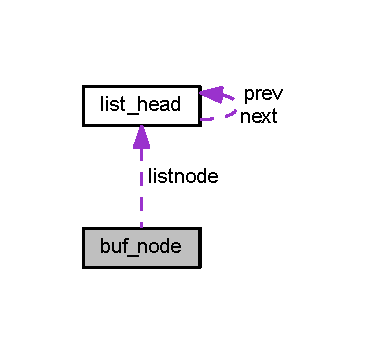
\includegraphics[width=175pt]{structbuf__node__coll__graph}
\end{center}
\end{figure}
\subsection*{Public Attributes}
\begin{DoxyCompactItemize}
\item 
\hypertarget{structbuf__node_aa143fa62d0856b406076c74ecb520a93}{}struct \hyperlink{structlist__head}{list\+\_\+head} {\bfseries listnode}\label{structbuf__node_aa143fa62d0856b406076c74ecb520a93}

\item 
\hypertarget{structbuf__node_aafb70b3757bcb414a8699d63605bc27b}{}char $\ast$ {\bfseries buf}\label{structbuf__node_aafb70b3757bcb414a8699d63605bc27b}

\item 
\hypertarget{structbuf__node_ab2ec24b8d0668ab8216e0845abe8355d}{}int {\bfseries buflen}\label{structbuf__node_ab2ec24b8d0668ab8216e0845abe8355d}

\end{DoxyCompactItemize}


The documentation for this struct was generated from the following file\+:\begin{DoxyCompactItemize}
\item 
D\+:/project/\+Peng\+Ge/client\+\_\+server/src/common/\hyperlink{buflist_8h}{buflist.\+h}\end{DoxyCompactItemize}

\hypertarget{structcsclient}{}\section{csclient Struct Reference}
\label{structcsclient}\index{csclient@{csclient}}


struct csclient contains necessary members and functions for client operations. This struct object must be initialized (by calling csclient\+\_\+init) before any operations applied to it.  




{\ttfamily \#include $<$client.\+h$>$}

\subsection*{Public Attributes}
\begin{DoxyCompactItemize}
\item 
\hypertarget{structcsclient_aa2665ff9ff09e43acae721376c92b9f4}{}int {\bfseries loggedin}\label{structcsclient_aa2665ff9ff09e43acae721376c92b9f4}

\item 
\hypertarget{structcsclient_ad730beb18ecbbb000950d8e1f7085d85}{}\hyperlink{sock__types_8h_aff065565f761db4433fff15fc7b7c471}{cssock\+\_\+t} {\bfseries hsock}\label{structcsclient_ad730beb18ecbbb000950d8e1f7085d85}

\item 
\hypertarget{structcsclient_a5e7b35f2d6dd38bd473ba94e35cbd9eb}{}struct sockaddr\+\_\+in \hyperlink{structcsclient_a5e7b35f2d6dd38bd473ba94e35cbd9eb}{sa\+\_\+in}\label{structcsclient_a5e7b35f2d6dd38bd473ba94e35cbd9eb}

\begin{DoxyCompactList}\small\item\em sockaddr\+\_\+in is the server socket address. \end{DoxyCompactList}\item 
\hypertarget{structcsclient_a40909df8825a1a5171688d280d98ebdb}{}char $\ast$ \hyperlink{structcsclient_a40909df8825a1a5171688d280d98ebdb}{prompt}\label{structcsclient_a40909df8825a1a5171688d280d98ebdb}

\begin{DoxyCompactList}\small\item\em msgheader is the string that print before message. For client, the msgheader is \char`\"{}client\char`\"{}, the output of client look like \char`\"{}clinet\+: xxx\char`\"{}. \end{DoxyCompactList}\item 
char \hyperlink{structcsclient_a325006ca2b5e74fe78e00847974234e5}{sendbuf} \mbox{[}M\+A\+X\+\_\+\+M\+S\+G\+\_\+\+L\+E\+N\mbox{]}
\begin{DoxyCompactList}\small\item\em sendbuf is the buffer to hold out message. \end{DoxyCompactList}\item 
\hypertarget{structcsclient_a2fd85113ce1bcbea4820f4b43ccdc761}{}int {\bfseries len\+\_\+senbuf}\label{structcsclient_a2fd85113ce1bcbea4820f4b43ccdc761}

\item 
char \hyperlink{structcsclient_a1ae9e95e2f7cb12d129776b0269ddae0}{recvbuf} \mbox{[}M\+A\+X\+\_\+\+M\+S\+G\+\_\+\+L\+E\+N\mbox{]}
\begin{DoxyCompactList}\small\item\em sendbuf is the buffer to hold the message from server. If size of message from server is greater than 1024 bytes, the client will cut off the tail contents and puts worning. \end{DoxyCompactList}\item 
\hypertarget{structcsclient_aad557f6df33e8820d04560ac9cbdfa5f}{}int {\bfseries len\+\_\+recvbuf}\label{structcsclient_aad557f6df33e8820d04560ac9cbdfa5f}

\end{DoxyCompactItemize}


\subsection{Detailed Description}
struct csclient contains necessary members and functions for client operations. This struct object must be initialized (by calling csclient\+\_\+init) before any operations applied to it. 

\begin{DoxySeeAlso}{See also}
\hyperlink{client_8h_a5aa275fcd29cc40dc4e8b04aca4836a8}{csclient\+\_\+init} 
\end{DoxySeeAlso}


\subsection{Member Data Documentation}
\hypertarget{structcsclient_a1ae9e95e2f7cb12d129776b0269ddae0}{}\index{csclient@{csclient}!recvbuf@{recvbuf}}
\index{recvbuf@{recvbuf}!csclient@{csclient}}
\subsubsection[{recvbuf}]{\setlength{\rightskip}{0pt plus 5cm}char csclient\+::recvbuf\mbox{[}M\+A\+X\+\_\+\+M\+S\+G\+\_\+\+L\+E\+N\mbox{]}}\label{structcsclient_a1ae9e95e2f7cb12d129776b0269ddae0}


sendbuf is the buffer to hold the message from server. If size of message from server is greater than 1024 bytes, the client will cut off the tail contents and puts worning. 

\begin{DoxyRefDesc}{Todo}
\item[\hyperlink{todo__todo000002}{Todo}]make recvbuf a pointer, and configure the length of recvbuf by user. \end{DoxyRefDesc}
\hypertarget{structcsclient_a325006ca2b5e74fe78e00847974234e5}{}\index{csclient@{csclient}!sendbuf@{sendbuf}}
\index{sendbuf@{sendbuf}!csclient@{csclient}}
\subsubsection[{sendbuf}]{\setlength{\rightskip}{0pt plus 5cm}char csclient\+::sendbuf\mbox{[}M\+A\+X\+\_\+\+M\+S\+G\+\_\+\+L\+E\+N\mbox{]}}\label{structcsclient_a325006ca2b5e74fe78e00847974234e5}


sendbuf is the buffer to hold out message. 

\begin{DoxyRefDesc}{Todo}
\item[\hyperlink{todo__todo000001}{Todo}]make sendbuf a pointer, and configure the length of sendbuf by user. \end{DoxyRefDesc}


The documentation for this struct was generated from the following file\+:\begin{DoxyCompactItemize}
\item 
D\+:/project/\+Peng\+Ge/client\+\_\+server/src/client/\hyperlink{client_8h}{client.\+h}\end{DoxyCompactItemize}

\hypertarget{structcsmsg__header}{}\section{csmsg\+\_\+header Struct Reference}
\label{structcsmsg__header}\index{csmsg\+\_\+header@{csmsg\+\_\+header}}


\hyperlink{structcsmsg__header}{csmsg\+\_\+header} describe the header in pool item. \hyperlink{structcsmsg__header}{csmsg\+\_\+header} is followed by the actual message data.  




{\ttfamily \#include $<$msgwrap.\+h$>$}



Collaboration diagram for csmsg\+\_\+header\+:
\nopagebreak
\begin{figure}[H]
\begin{center}
\leavevmode
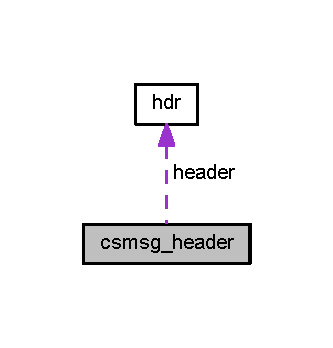
\includegraphics[width=160pt]{structcsmsg__header__coll__graph}
\end{center}
\end{figure}
\subsection*{Public Attributes}
\begin{DoxyCompactItemize}
\item 
\hypertarget{structcsmsg__header_aa250b3612f8722982b2418ebc173ac07}{}struct sockaddr {\bfseries addr}\label{structcsmsg__header_aa250b3612f8722982b2418ebc173ac07}

\item 
\hypertarget{structcsmsg__header_aaf0f1d34d725622d45ebcd83de7eb98c}{}int {\bfseries addrlen}\label{structcsmsg__header_aaf0f1d34d725622d45ebcd83de7eb98c}

\item 
\hypertarget{structcsmsg__header_afe5ffaa8a10ca3c8f7ab9fc1d9e33326}{}struct \hyperlink{structhdr}{hdr} {\bfseries header}\label{structcsmsg__header_afe5ffaa8a10ca3c8f7ab9fc1d9e33326}

\item 
\hypertarget{structcsmsg__header_a341e25526736f6805d4b4b29c088da73}{}int {\bfseries numbytes}\label{structcsmsg__header_a341e25526736f6805d4b4b29c088da73}

\end{DoxyCompactItemize}


\subsection{Detailed Description}
\hyperlink{structcsmsg__header}{csmsg\+\_\+header} describe the header in pool item. \hyperlink{structcsmsg__header}{csmsg\+\_\+header} is followed by the actual message data. 

The documentation for this struct was generated from the following file\+:\begin{DoxyCompactItemize}
\item 
D\+:/project/\+Peng\+Ge/client\+\_\+server/src/common/\hyperlink{msgwrap_8h}{msgwrap.\+h}\end{DoxyCompactItemize}

\hypertarget{structcsmsgpool}{}\section{csmsgpool Struct Reference}
\label{structcsmsgpool}\index{csmsgpool@{csmsgpool}}


csmsgpool contains basic members for send receive buffer and thread operations. The members of struct csmsgpool should be set with configuration.  




{\ttfamily \#include $<$msgpool.\+h$>$}



Collaboration diagram for csmsgpool\+:
\nopagebreak
\begin{figure}[H]
\begin{center}
\leavevmode
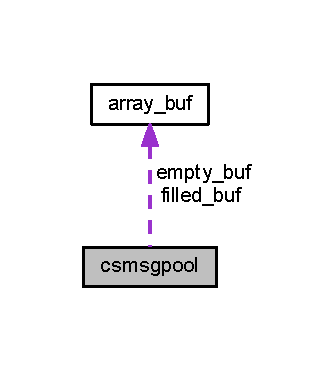
\includegraphics[width=161pt]{structcsmsgpool__coll__graph}
\end{center}
\end{figure}
\subsection*{Public Attributes}
\begin{DoxyCompactItemize}
\item 
\hypertarget{structcsmsgpool_a3a54f33ded9e2dca3aae11bd2360d4f5}{}int {\bfseries num\+\_\+thread}\label{structcsmsgpool_a3a54f33ded9e2dca3aae11bd2360d4f5}

\item 
\hypertarget{structcsmsgpool_a18960e59cac87bd3db96978b5ad01ce5}{}int {\bfseries len\+\_\+item}\label{structcsmsgpool_a18960e59cac87bd3db96978b5ad01ce5}

\item 
\hypertarget{structcsmsgpool_a4fc562000466f47cd9dc3e4f58ea9b15}{}int {\bfseries num\+\_\+item}\label{structcsmsgpool_a4fc562000466f47cd9dc3e4f58ea9b15}

\item 
\hypertarget{structcsmsgpool_a1828032c5206f6d03095c133575f010f}{}struct \hyperlink{structarray__buf}{array\+\_\+buf} {\bfseries filled\+\_\+buf}\label{structcsmsgpool_a1828032c5206f6d03095c133575f010f}

\item 
\hypertarget{structcsmsgpool_a5cb22f9beccddb5a7177719a6f97c7f3}{}struct \hyperlink{structarray__buf}{array\+\_\+buf} {\bfseries empty\+\_\+buf}\label{structcsmsgpool_a5cb22f9beccddb5a7177719a6f97c7f3}

\item 
\hypertarget{structcsmsgpool_ab2f992ea0595aecf88e68939a5a742c1}{}\hyperlink{sock__types_8h_aff065565f761db4433fff15fc7b7c471}{cssock\+\_\+t} \hyperlink{structcsmsgpool_ab2f992ea0595aecf88e68939a5a742c1}{socket}\label{structcsmsgpool_ab2f992ea0595aecf88e68939a5a742c1}

\begin{DoxyCompactList}\small\item\em socket \end{DoxyCompactList}\item 
\hypertarget{structcsmsgpool_a990d35a81d5e6e8823029fd0f4d8c3d4}{}csmutex\+\_\+t \hyperlink{structcsmsgpool_a990d35a81d5e6e8823029fd0f4d8c3d4}{hmutex}\label{structcsmsgpool_a990d35a81d5e6e8823029fd0f4d8c3d4}

\begin{DoxyCompactList}\small\item\em hmutex \end{DoxyCompactList}\item 
\hypertarget{structcsmsgpool_af85d9571d64d3471517331ce9c1f16a2}{}csthread\+\_\+t $\ast$ \hyperlink{structcsmsgpool_af85d9571d64d3471517331ce9c1f16a2}{hthread}\label{structcsmsgpool_af85d9571d64d3471517331ce9c1f16a2}

\begin{DoxyCompactList}\small\item\em hthread \end{DoxyCompactList}\item 
int \hyperlink{structcsmsgpool_a7d814c8195e4baacad1f4045c8e63ad8}{threadexit}
\begin{DoxyCompactList}\small\item\em threadexit threadexit is used to make thread exit normally. If threadexit is 1, thread will exit; if threadexit is 0, thread keep on running. \end{DoxyCompactList}\item 
\hypertarget{structcsmsgpool_a3e8ddb48e68c25fb6874520af10d58be}{}cssem\+\_\+t \hyperlink{structcsmsgpool_a3e8ddb48e68c25fb6874520af10d58be}{hsem\+\_\+filled}\label{structcsmsgpool_a3e8ddb48e68c25fb6874520af10d58be}

\begin{DoxyCompactList}\small\item\em hsem\+\_\+filled Be careful, csmsgpool call cssem\+\_\+wait() and cssem\+\_\+post() by default. \end{DoxyCompactList}\item 
int \hyperlink{structcsmsgpool_ab79b44d003c02515c83d5772eb53c937}{use\+\_\+sem\+\_\+in\+\_\+pool}
\begin{DoxyCompactList}\small\item\em use\+\_\+sem\+\_\+in\+\_\+pool 1 turn on semaphore wait or post, 0 turn off. \end{DoxyCompactList}\end{DoxyCompactItemize}


\subsection{Detailed Description}
csmsgpool contains basic members for send receive buffer and thread operations. The members of struct csmsgpool should be set with configuration. 

\begin{DoxyRefDesc}{Todo}
\item[\hyperlink{todo__todo000003}{Todo}]write a cofigure parser to set the members \end{DoxyRefDesc}


\subsection{Member Data Documentation}
\hypertarget{structcsmsgpool_a7d814c8195e4baacad1f4045c8e63ad8}{}\index{csmsgpool@{csmsgpool}!threadexit@{threadexit}}
\index{threadexit@{threadexit}!csmsgpool@{csmsgpool}}
\subsubsection[{threadexit}]{\setlength{\rightskip}{0pt plus 5cm}int csmsgpool\+::threadexit}\label{structcsmsgpool_a7d814c8195e4baacad1f4045c8e63ad8}


threadexit threadexit is used to make thread exit normally. If threadexit is 1, thread will exit; if threadexit is 0, thread keep on running. 

\begin{DoxyNote}{Note}
thread entry must test this value to determine whether exit or not, as the following code shows.
\end{DoxyNote}

\begin{DoxyCode}
func()
\{
    \textcolor{keywordflow}{while} (1) \{
        \textcolor{keywordflow}{if} (\hyperlink{structcsmsgpool_a7d814c8195e4baacad1f4045c8e63ad8}{threadexit}) \{
            \textcolor{keywordflow}{break};
        \}
    \}
\}
\end{DoxyCode}
 \hypertarget{structcsmsgpool_ab79b44d003c02515c83d5772eb53c937}{}\index{csmsgpool@{csmsgpool}!use\+\_\+sem\+\_\+in\+\_\+pool@{use\+\_\+sem\+\_\+in\+\_\+pool}}
\index{use\+\_\+sem\+\_\+in\+\_\+pool@{use\+\_\+sem\+\_\+in\+\_\+pool}!csmsgpool@{csmsgpool}}
\subsubsection[{use\+\_\+sem\+\_\+in\+\_\+pool}]{\setlength{\rightskip}{0pt plus 5cm}int csmsgpool\+::use\+\_\+sem\+\_\+in\+\_\+pool}\label{structcsmsgpool_ab79b44d003c02515c83d5772eb53c937}


use\+\_\+sem\+\_\+in\+\_\+pool 1 turn on semaphore wait or post, 0 turn off. 

\begin{DoxyNote}{Note}
use\+\_\+sem\+\_\+in\+\_\+pool only works in cspool\+\_\+pulldata and cspool\+\_\+pushdata. user shoud call semaphore wait and post explicit while calling cspool\+\_\+pullitem and cspool\+\_\+pushitem. 
\end{DoxyNote}


The documentation for this struct was generated from the following file\+:\begin{DoxyCompactItemize}
\item 
D\+:/project/\+Peng\+Ge/client\+\_\+server/src/common/\hyperlink{msgpool_8h}{msgpool.\+h}\end{DoxyCompactItemize}

\hypertarget{structcsmsgpool__dispatch}{}\section{csmsgpool\+\_\+dispatch Struct Reference}
\label{structcsmsgpool__dispatch}\index{csmsgpool\+\_\+dispatch@{csmsgpool\+\_\+dispatch}}


Collaboration diagram for csmsgpool\+\_\+dispatch\+:
\nopagebreak
\begin{figure}[H]
\begin{center}
\leavevmode
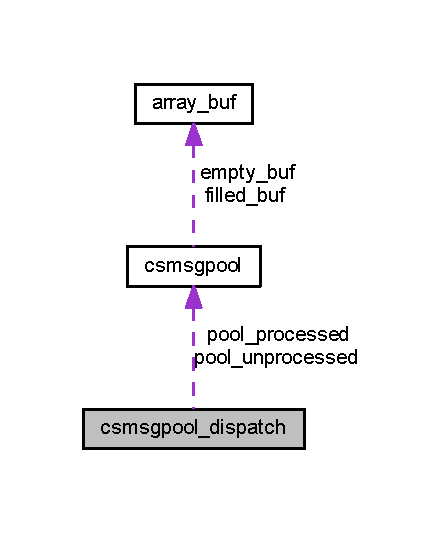
\includegraphics[width=212pt]{structcsmsgpool__dispatch__coll__graph}
\end{center}
\end{figure}
\subsection*{Public Attributes}
\begin{DoxyCompactItemize}
\item 
\hypertarget{structcsmsgpool__dispatch_a93ea8159cd6de7995c4ad5616cdb2c4b}{}char $\ast$ {\bfseries prompt}\label{structcsmsgpool__dispatch_a93ea8159cd6de7995c4ad5616cdb2c4b}

\item 
\hypertarget{structcsmsgpool__dispatch_a9b02b2e04339a0b32c78a21f8fee8a46}{}struct \hyperlink{structcsmsgpool}{csmsgpool} {\bfseries pool\+\_\+unprocessed}\label{structcsmsgpool__dispatch_a9b02b2e04339a0b32c78a21f8fee8a46}

\item 
struct \hyperlink{structcsmsgpool}{csmsgpool} \hyperlink{structcsmsgpool__dispatch_adcf1e4f0175a47fcfc0283971dbdef57}{pool\+\_\+processed}
\begin{DoxyCompactList}\small\item\em This pool can be ignored if immediately sending data is not required after process. \end{DoxyCompactList}\item 
\hypertarget{structcsmsgpool__dispatch_aefa9098045031a5af9561633c8ff3c10}{}csmsg\+\_\+process\+\_\+t $\ast$ \hyperlink{structcsmsgpool__dispatch_aefa9098045031a5af9561633c8ff3c10}{process\+\_\+msg}\label{structcsmsgpool__dispatch_aefa9098045031a5af9561633c8ff3c10}

\begin{DoxyCompactList}\small\item\em process\+\_\+msg This variable must be set to point a function. \end{DoxyCompactList}\item 
\hypertarget{structcsmsgpool__dispatch_a71e3b4138d0c8952ee6353a1992e26f2}{}csmsg\+\_\+process\+\_\+af\+\_\+t $\ast$ \hyperlink{structcsmsgpool__dispatch_a71e3b4138d0c8952ee6353a1992e26f2}{process\+\_\+af\+\_\+msg}\label{structcsmsgpool__dispatch_a71e3b4138d0c8952ee6353a1992e26f2}

\begin{DoxyCompactList}\small\item\em process\+\_\+af\+\_\+msg If send message is not required after process, set process\+\_\+af\+\_\+msg to 0; \end{DoxyCompactList}\item 
\hypertarget{structcsmsgpool__dispatch_afd343a0b051450dd308226f6e2c8f9a7}{}void $\ast$ {\bfseries process\+\_\+pargs}\label{structcsmsgpool__dispatch_afd343a0b051450dd308226f6e2c8f9a7}

\end{DoxyCompactItemize}


\subsection{Member Data Documentation}
\hypertarget{structcsmsgpool__dispatch_adcf1e4f0175a47fcfc0283971dbdef57}{}\index{csmsgpool\+\_\+dispatch@{csmsgpool\+\_\+dispatch}!pool\+\_\+processed@{pool\+\_\+processed}}
\index{pool\+\_\+processed@{pool\+\_\+processed}!csmsgpool\+\_\+dispatch@{csmsgpool\+\_\+dispatch}}
\subsubsection[{pool\+\_\+processed}]{\setlength{\rightskip}{0pt plus 5cm}struct {\bf csmsgpool} csmsgpool\+\_\+dispatch\+::pool\+\_\+processed}\label{structcsmsgpool__dispatch_adcf1e4f0175a47fcfc0283971dbdef57}


This pool can be ignored if immediately sending data is not required after process. 

\begin{DoxySeeAlso}{See also}
semd\+\_\+msg 
\end{DoxySeeAlso}


The documentation for this struct was generated from the following file\+:\begin{DoxyCompactItemize}
\item 
D\+:/project/\+Peng\+Ge/client\+\_\+server/src/common/\hyperlink{msgpool__dispatch_8h}{msgpool\+\_\+dispatch.\+h}\end{DoxyCompactItemize}

\hypertarget{structcsserver}{}\section{csserver Struct Reference}
\label{structcsserver}\index{csserver@{csserver}}
\subsection*{Public Attributes}
\begin{DoxyCompactItemize}
\item 
\hypertarget{structcsserver_a85d00fe1d4afb6628c32544533a982d9}{}\hyperlink{sock__types_8h_aff065565f761db4433fff15fc7b7c471}{cssock\+\_\+t} {\bfseries hsock}\label{structcsserver_a85d00fe1d4afb6628c32544533a982d9}

\item 
\hypertarget{structcsserver_a0bafc662541f5a0772341a60e109f99b}{}struct sockaddr\+\_\+in {\bfseries sa\+\_\+in}\label{structcsserver_a0bafc662541f5a0772341a60e109f99b}

\item 
\hypertarget{structcsserver_a9f9d1438336232441c95191ea11c3b5c}{}char $\ast$ {\bfseries prompt}\label{structcsserver_a9f9d1438336232441c95191ea11c3b5c}

\end{DoxyCompactItemize}


The documentation for this struct was generated from the following file\+:\begin{DoxyCompactItemize}
\item 
D\+:/project/\+Peng\+Ge/client\+\_\+server/src/server/\hyperlink{server_8h}{server.\+h}\end{DoxyCompactItemize}

\hypertarget{structhdr}{}\section{hdr Struct Reference}
\label{structhdr}\index{hdr@{hdr}}
\subsection*{Public Attributes}
\begin{DoxyCompactItemize}
\item 
\hypertarget{structhdr_a0fe6fdc43d5884531407540c317cc29a}{}uint32\+\_\+t {\bfseries seg}\label{structhdr_a0fe6fdc43d5884531407540c317cc29a}

\item 
\hypertarget{structhdr_a0902aeb74b0763203be1c07c2cbc10da}{}uint32\+\_\+t {\bfseries ts}\label{structhdr_a0902aeb74b0763203be1c07c2cbc10da}

\end{DoxyCompactItemize}


The documentation for this struct was generated from the following file\+:\begin{DoxyCompactItemize}
\item 
D\+:/\+Projects/\+Peng\+Ge/client\+\_\+server/\+Qt\+\_\+winsock/common/\hyperlink{udp__types_8h}{udp\+\_\+types.\+h}\end{DoxyCompactItemize}

\hypertarget{structlist__head}{}\section{list\+\_\+head Struct Reference}
\label{structlist__head}\index{list\+\_\+head@{list\+\_\+head}}


Collaboration diagram for list\+\_\+head\+:
\nopagebreak
\begin{figure}[H]
\begin{center}
\leavevmode
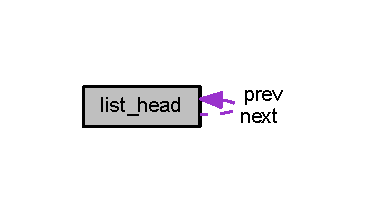
\includegraphics[width=175pt]{structlist__head__coll__graph}
\end{center}
\end{figure}
\subsection*{Public Attributes}
\begin{DoxyCompactItemize}
\item 
\hypertarget{structlist__head_ac3b0ff0dfb978a0cfbdad6b9d19cdcfe}{}struct \hyperlink{structlist__head}{list\+\_\+head} $\ast$ {\bfseries next}\label{structlist__head_ac3b0ff0dfb978a0cfbdad6b9d19cdcfe}

\item 
\hypertarget{structlist__head_aaa0eabda8877e1d6de73a33f223ad004}{}struct \hyperlink{structlist__head}{list\+\_\+head} $\ast$ {\bfseries prev}\label{structlist__head_aaa0eabda8877e1d6de73a33f223ad004}

\end{DoxyCompactItemize}


The documentation for this struct was generated from the following file\+:\begin{DoxyCompactItemize}
\item 
D\+:/project/\+Peng\+Ge/client\+\_\+server/src/common/\hyperlink{list_8h}{list.\+h}\end{DoxyCompactItemize}

\hypertarget{structrtt__info}{}\section{rtt\+\_\+info Struct Reference}
\label{structrtt__info}\index{rtt\+\_\+info@{rtt\+\_\+info}}
\subsection*{Public Attributes}
\begin{DoxyCompactItemize}
\item 
\hypertarget{structrtt__info_a63cf11310859ddccb8927225f3547b30}{}float {\bfseries rtt\+\_\+rtt}\label{structrtt__info_a63cf11310859ddccb8927225f3547b30}

\item 
\hypertarget{structrtt__info_a10236c8eb80b30f1d37d44ccc449eddb}{}float {\bfseries rtt\+\_\+srtt}\label{structrtt__info_a10236c8eb80b30f1d37d44ccc449eddb}

\item 
\hypertarget{structrtt__info_a606ee3fa94939f59b7bde1623de059c9}{}float {\bfseries rtt\+\_\+rttvar}\label{structrtt__info_a606ee3fa94939f59b7bde1623de059c9}

\item 
\hypertarget{structrtt__info_a4872c2830891ce21535646376c4311cf}{}float {\bfseries rtt\+\_\+rto}\label{structrtt__info_a4872c2830891ce21535646376c4311cf}

\item 
\hypertarget{structrtt__info_a19ec3e43f0bff53ea5a0d39025b7f9ae}{}int {\bfseries rtt\+\_\+nrexmt}\label{structrtt__info_a19ec3e43f0bff53ea5a0d39025b7f9ae}

\item 
\hypertarget{structrtt__info_a552a6d4f8a5c78271145b30e31a72630}{}uint32\+\_\+t {\bfseries rtt\+\_\+base}\label{structrtt__info_a552a6d4f8a5c78271145b30e31a72630}

\end{DoxyCompactItemize}


The documentation for this struct was generated from the following file\+:\begin{DoxyCompactItemize}
\item 
D\+:/project/\+Peng\+Ge/client\+\_\+server/src/common/\hyperlink{unprtt_8h}{unprtt.\+h}\end{DoxyCompactItemize}

\hypertarget{structsock__option}{}\section{sock\+\_\+option Struct Reference}
\label{structsock__option}\index{sock\+\_\+option@{sock\+\_\+option}}
\subsection*{Public Attributes}
\begin{DoxyCompactItemize}
\item 
\hypertarget{structsock__option_a38173c15ab8d3ebcd413c616324a4d83}{}int {\bfseries block}\label{structsock__option_a38173c15ab8d3ebcd413c616324a4d83}

\item 
\hypertarget{structsock__option_ad59873211046162ae364ef427add81dd}{}int {\bfseries size\+\_\+sendbuf}\label{structsock__option_ad59873211046162ae364ef427add81dd}

\item 
\hypertarget{structsock__option_aaf1c039657331eaab8770c6453123760}{}int {\bfseries size\+\_\+recvbuf}\label{structsock__option_aaf1c039657331eaab8770c6453123760}

\end{DoxyCompactItemize}


The documentation for this struct was generated from the following file\+:\begin{DoxyCompactItemize}
\item 
D\+:/project/\+Peng\+Ge/client\+\_\+server/src/common/\hyperlink{sock__types_8h}{sock\+\_\+types.\+h}\end{DoxyCompactItemize}

\chapter{File Documentation}
\hypertarget{main__arraybuf_8c}{}\section{D\+:/project/\+Peng\+Ge/client\+\_\+server/samples/test\+\_\+threadpool/main\+\_\+arraybuf.c File Reference}
\label{main__arraybuf_8c}\index{D\+:/project/\+Peng\+Ge/client\+\_\+server/samples/test\+\_\+threadpool/main\+\_\+arraybuf.\+c@{D\+:/project/\+Peng\+Ge/client\+\_\+server/samples/test\+\_\+threadpool/main\+\_\+arraybuf.\+c}}


This demo routine use \textquotesingle{}struct \hyperlink{structarray__buf}{array\+\_\+buf}\textquotesingle{} as the buffer struct.  


{\ttfamily \#include $<$pthread.\+h$>$}\\*
{\ttfamily \#include $<$semaphore.\+h$>$}\\*
{\ttfamily \#include $<$assert.\+h$>$}\\*
{\ttfamily \#include $<$stdio.\+h$>$}\\*
{\ttfamily \#include \char`\"{}macros.\+h\char`\"{}}\\*
{\ttfamily \#include \char`\"{}bufarray.\+h\char`\"{}}\\*
{\ttfamily \#include \char`\"{}lightthread.\+h\char`\"{}}\\*
Include dependency graph for main\+\_\+arraybuf.\+c\+:
\nopagebreak
\begin{figure}[H]
\begin{center}
\leavevmode
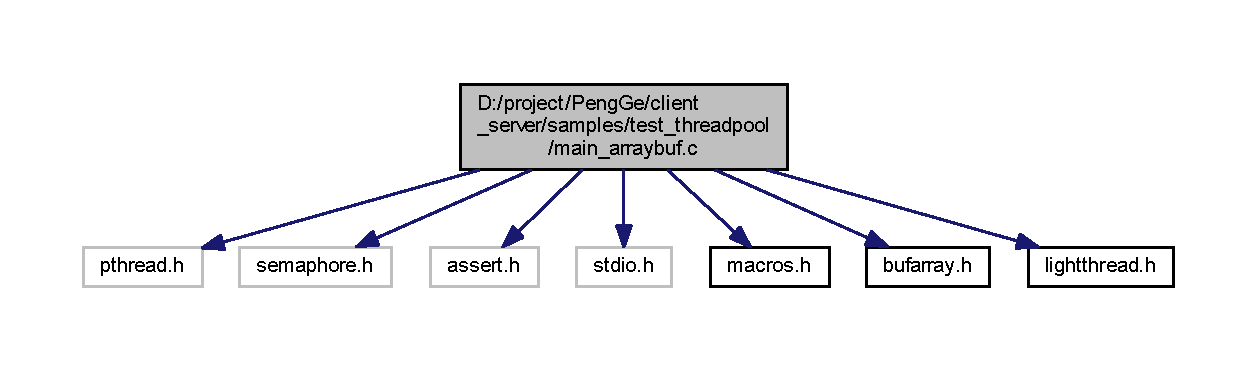
\includegraphics[width=350pt]{main__arraybuf_8c__incl}
\end{center}
\end{figure}
\subsection*{Macros}
\begin{DoxyCompactItemize}
\item 
\hypertarget{main__arraybuf_8c_adfe18adc4528f82b5f2e57633b31c084}{}\#define {\bfseries N\+U\+M\+\_\+\+T\+H\+R\+E\+A\+D}~4\label{main__arraybuf_8c_adfe18adc4528f82b5f2e57633b31c084}

\end{DoxyCompactItemize}
\subsection*{Functions}
\begin{DoxyCompactItemize}
\item 
\hypertarget{main__arraybuf_8c_a840291bc02cba5474a4cb46a9b9566fe}{}int {\bfseries main} (void)\label{main__arraybuf_8c_a840291bc02cba5474a4cb46a9b9566fe}

\end{DoxyCompactItemize}
\subsection*{Variables}
\begin{DoxyCompactItemize}
\item 
\hypertarget{main__arraybuf_8c_a9143008a69af4305e80f8a56a5f74146}{}csmutex\+\_\+t {\bfseries hmutex}\label{main__arraybuf_8c_a9143008a69af4305e80f8a56a5f74146}

\item 
\hypertarget{main__arraybuf_8c_a160a3e85f4be09865973981be298ffdc}{}cssem\+\_\+t {\bfseries hsem\+\_\+filled}\label{main__arraybuf_8c_a160a3e85f4be09865973981be298ffdc}

\item 
\hypertarget{main__arraybuf_8c_aa024d7e99e168ef21eb31c241cd3c020}{}csthread\+\_\+t {\bfseries hthreads} \mbox{[}N\+U\+M\+\_\+\+T\+H\+R\+E\+A\+D\mbox{]}\label{main__arraybuf_8c_aa024d7e99e168ef21eb31c241cd3c020}

\item 
\hypertarget{main__arraybuf_8c_a29c10ccc9ec54b8154255fae5d6a2a0e}{}char {\bfseries buf} \mbox{[}255\mbox{]}\label{main__arraybuf_8c_a29c10ccc9ec54b8154255fae5d6a2a0e}

\end{DoxyCompactItemize}


\subsection{Detailed Description}
This demo routine use \textquotesingle{}struct \hyperlink{structarray__buf}{array\+\_\+buf}\textquotesingle{} as the buffer struct. 

\begin{DoxyAuthor}{Author}
cxl, \href{mailto:shuanglongchen@yeah.net}{\tt shuanglongchen@yeah.\+net} 
\end{DoxyAuthor}
\begin{DoxyVersion}{Version}
0.\+1 
\end{DoxyVersion}
\begin{DoxyDate}{Date}
2015-\/10-\/17 
\end{DoxyDate}

\hypertarget{client_8c}{}\section{D\+:/project/\+Peng\+Ge/client\+\_\+server/src/client/client.c File Reference}
\label{client_8c}\index{D\+:/project/\+Peng\+Ge/client\+\_\+server/src/client/client.\+c@{D\+:/project/\+Peng\+Ge/client\+\_\+server/src/client/client.\+c}}
{\ttfamily \#include $<$setjmp.\+h$>$}\\*
{\ttfamily \#include $<$signal.\+h$>$}\\*
{\ttfamily \#include $<$sys/socket.\+h$>$}\\*
{\ttfamily \#include $<$netinet/in.\+h$>$}\\*
{\ttfamily \#include $<$stdint.\+h$>$}\\*
{\ttfamily \#include $<$stdio.\+h$>$}\\*
{\ttfamily \#include $<$stdlib.\+h$>$}\\*
{\ttfamily \#include $<$string.\+h$>$}\\*
{\ttfamily \#include \char`\"{}macros.\+h\char`\"{}}\\*
{\ttfamily \#include \char`\"{}sock\+\_\+types.\+h\char`\"{}}\\*
{\ttfamily \#include \char`\"{}error.\+h\char`\"{}}\\*
{\ttfamily \#include \char`\"{}client.\+h\char`\"{}}\\*
{\ttfamily \#include \char`\"{}sock\+\_\+wrap.\+h\char`\"{}}\\*
Include dependency graph for client.\+c\+:
\nopagebreak
\begin{figure}[H]
\begin{center}
\leavevmode
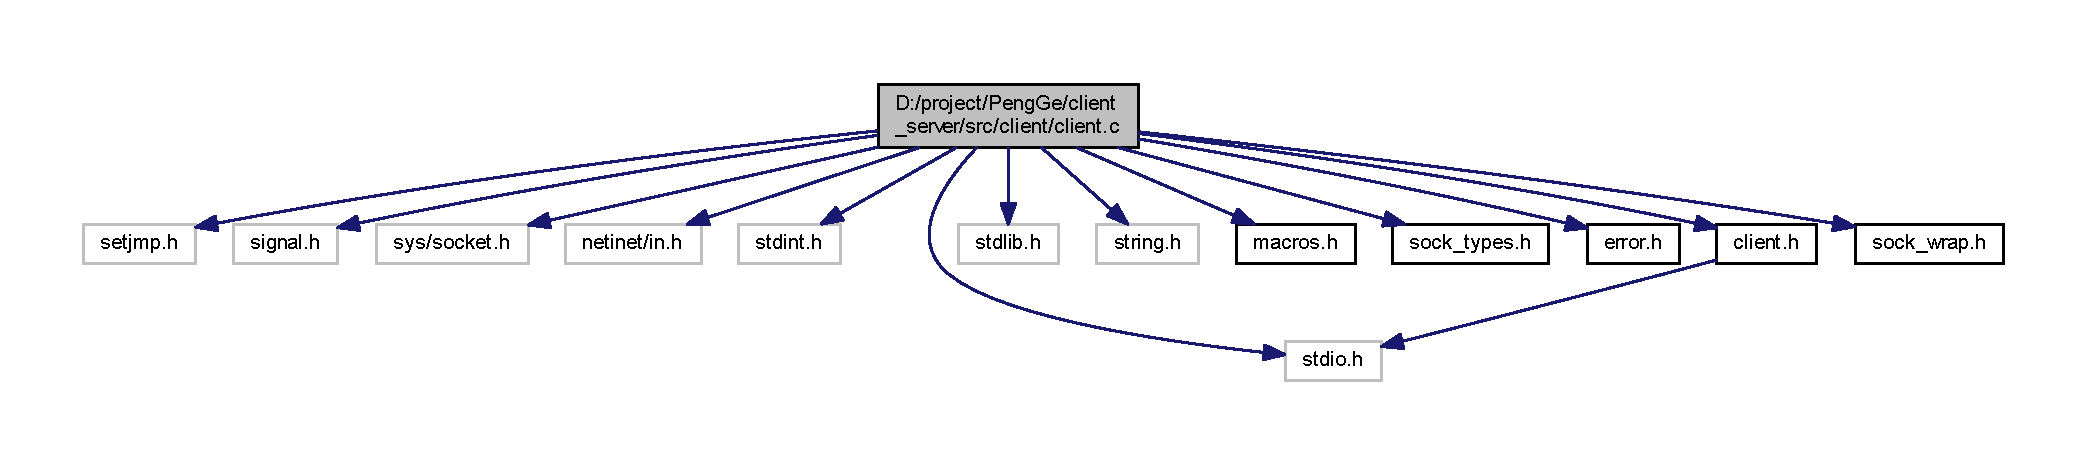
\includegraphics[width=350pt]{client_8c__incl}
\end{center}
\end{figure}
\subsection*{Functions}
\begin{DoxyCompactItemize}
\item 
void \hyperlink{client_8c_a5aa275fcd29cc40dc4e8b04aca4836a8}{csclient\+\_\+init} (struct \hyperlink{structcsclient}{csclient} $\ast$cli, int tcpudp)
\begin{DoxyCompactList}\small\item\em csclient\+\_\+init \end{DoxyCompactList}\item 
void \hyperlink{client_8c_ae3752395d79c6d9a2920d96c73eb81ed}{csclient\+\_\+clear} (struct \hyperlink{structcsclient}{csclient} $\ast$cli)
\begin{DoxyCompactList}\small\item\em csclient\+\_\+clear There may be some clear works after communication, such as free the memory. \end{DoxyCompactList}\item 
int \hyperlink{client_8c_aa263fe24e3c96c3a1b1b8c087eb518b7}{csclient\+\_\+print} (const struct \hyperlink{structcsclient}{csclient} $\ast$cli)
\begin{DoxyCompactList}\small\item\em csclient\+\_\+print csclient\+\_\+print will test and print client socket information. If test fail, process will clear the socket environmtn and exit. \end{DoxyCompactList}\item 
\hypertarget{client_8c_a20e5a0eb2e564b26d13f5ab34c1a5986}{}void {\bfseries csclient\+\_\+connect} (struct \hyperlink{structcsclient}{csclient} $\ast$cli, const struct sockaddr $\ast$servaddr, cssocklen\+\_\+t addrlen)\label{client_8c_a20e5a0eb2e564b26d13f5ab34c1a5986}

\end{DoxyCompactItemize}
\subsection*{Variables}
\begin{DoxyCompactItemize}
\item 
\hypertarget{client_8c_a2b0ae9a11011f0505defee4c3575b5b2}{}int {\bfseries g\+\_\+cli\+\_\+sendbuflen}\label{client_8c_a2b0ae9a11011f0505defee4c3575b5b2}

\item 
\hypertarget{client_8c_ab3de0e2c75c8081c7b9860a0c0e6cbb8}{}int {\bfseries g\+\_\+cli\+\_\+recvbuflen}\label{client_8c_ab3de0e2c75c8081c7b9860a0c0e6cbb8}

\end{DoxyCompactItemize}


\subsection{Detailed Description}
\begin{DoxyAuthor}{Author}
cxl, \href{mailto:shuanglongchen@yeah.net}{\tt shuanglongchen@yeah.\+net} 
\end{DoxyAuthor}
\begin{DoxyVersion}{Version}
0.\+1 
\end{DoxyVersion}
\begin{DoxyDate}{Date}
2015-\/09-\/30 
\end{DoxyDate}
\begin{DoxyParagraph}{last modified}
Sat 2015-\/11-\/07 13\+:30\+:58 (+0800) 
\end{DoxyParagraph}


\subsection{Function Documentation}
\hypertarget{client_8c_ae3752395d79c6d9a2920d96c73eb81ed}{}\index{client.\+c@{client.\+c}!csclient\+\_\+clear@{csclient\+\_\+clear}}
\index{csclient\+\_\+clear@{csclient\+\_\+clear}!client.\+c@{client.\+c}}
\subsubsection[{csclient\+\_\+clear(struct csclient $\ast$cli)}]{\setlength{\rightskip}{0pt plus 5cm}void csclient\+\_\+clear (
\begin{DoxyParamCaption}
\item[{struct {\bf csclient} $\ast$}]{cli}
\end{DoxyParamCaption}
)}\label{client_8c_ae3752395d79c6d9a2920d96c73eb81ed}


csclient\+\_\+clear There may be some clear works after communication, such as free the memory. 


\begin{DoxyParams}{Parameters}
{\em cli} & \\
\hline
\end{DoxyParams}
\hypertarget{client_8c_a5aa275fcd29cc40dc4e8b04aca4836a8}{}\index{client.\+c@{client.\+c}!csclient\+\_\+init@{csclient\+\_\+init}}
\index{csclient\+\_\+init@{csclient\+\_\+init}!client.\+c@{client.\+c}}
\subsubsection[{csclient\+\_\+init(struct csclient $\ast$cli, int tcpudp)}]{\setlength{\rightskip}{0pt plus 5cm}void csclient\+\_\+init (
\begin{DoxyParamCaption}
\item[{struct {\bf csclient} $\ast$}]{cli, }
\item[{int}]{tcpudp}
\end{DoxyParamCaption}
)}\label{client_8c_a5aa275fcd29cc40dc4e8b04aca4836a8}


csclient\+\_\+init 


\begin{DoxyParams}{Parameters}
{\em cli} & \\
\hline
{\em tcpudp} & Tcp socket will be created if S\+O\+C\+K\+\_\+\+S\+T\+R\+E\+A\+M is set, upd socket will be created if S\+O\+C\+K\+\_\+\+D\+G\+R\+A\+M is set.\\
\hline
\end{DoxyParams}
\begin{DoxyNote}{Note}

\begin{DoxyEnumerate}
\item This function must be called after init\+\_\+sock\+\_\+environment being called.
\item Socket is set to be non-\/blocking socket by default. Call cssock\+\_\+block explicitly if you need the socket to be blocking.
\end{DoxyEnumerate}
\end{DoxyNote}
\begin{DoxySeeAlso}{See also}
\hyperlink{sock__wrap_8h_a60b0fd1896802faae9fd9dd341fadc54}{cssock\+\_\+block} \hyperlink{sock__wrap_8h_a842dda0d61b2e39aab64b40764adddd1}{cssock\+\_\+open} 
\end{DoxySeeAlso}


Here is the call graph for this function\+:
\nopagebreak
\begin{figure}[H]
\begin{center}
\leavevmode
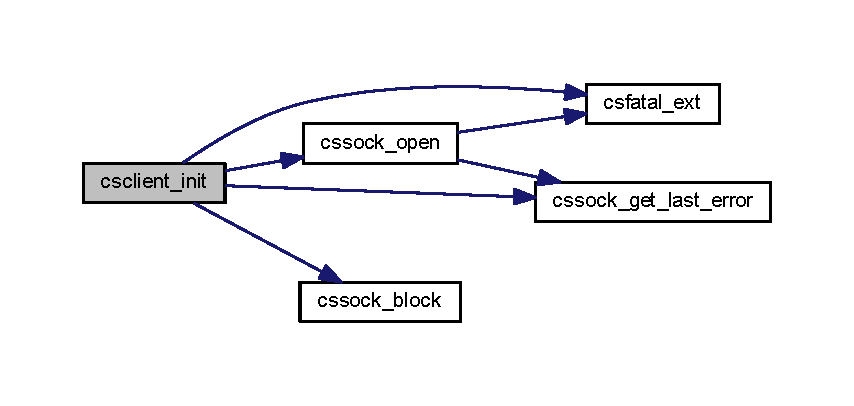
\includegraphics[width=350pt]{client_8c_a5aa275fcd29cc40dc4e8b04aca4836a8_cgraph}
\end{center}
\end{figure}


\hypertarget{client_8c_aa263fe24e3c96c3a1b1b8c087eb518b7}{}\index{client.\+c@{client.\+c}!csclient\+\_\+print@{csclient\+\_\+print}}
\index{csclient\+\_\+print@{csclient\+\_\+print}!client.\+c@{client.\+c}}
\subsubsection[{csclient\+\_\+print(const struct csclient $\ast$cli)}]{\setlength{\rightskip}{0pt plus 5cm}int csclient\+\_\+print (
\begin{DoxyParamCaption}
\item[{const struct {\bf csclient} $\ast$}]{cli}
\end{DoxyParamCaption}
)}\label{client_8c_aa263fe24e3c96c3a1b1b8c087eb518b7}


csclient\+\_\+print csclient\+\_\+print will test and print client socket information. If test fail, process will clear the socket environmtn and exit. 


\begin{DoxyParams}{Parameters}
{\em cli} & \\
\hline
\end{DoxyParams}
\begin{DoxyReturn}{Returns}

\begin{DoxyEnumerate}
\item -\/1, if socket is not a valid socket.
\item 0, if socket is connected.
\item 1, if socket is not connected.
\end{DoxyEnumerate}
\end{DoxyReturn}
\begin{DoxySeeAlso}{See also}
\hyperlink{sock__wrap_8h_a047455240499ada0472e5722cd50640b}{cssock\+\_\+print} 
\end{DoxySeeAlso}


Here is the call graph for this function\+:
\nopagebreak
\begin{figure}[H]
\begin{center}
\leavevmode
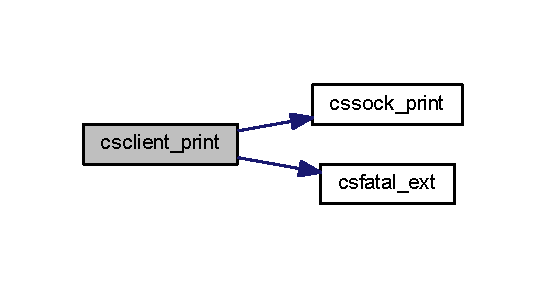
\includegraphics[width=262pt]{client_8c_aa263fe24e3c96c3a1b1b8c087eb518b7_cgraph}
\end{center}
\end{figure}



\hypertarget{client_8h}{}\section{D\+:/project/\+Peng\+Ge/client\+\_\+server/src/client/client.h File Reference}
\label{client_8h}\index{D\+:/project/\+Peng\+Ge/client\+\_\+server/src/client/client.\+h@{D\+:/project/\+Peng\+Ge/client\+\_\+server/src/client/client.\+h}}


This file provide the basic helper funstion for client struct.  


{\ttfamily \#include $<$stdio.\+h$>$}\\*
Include dependency graph for client.\+h\+:
\nopagebreak
\begin{figure}[H]
\begin{center}
\leavevmode
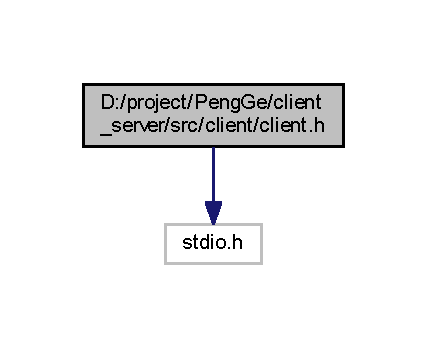
\includegraphics[width=205pt]{client_8h__incl}
\end{center}
\end{figure}
This graph shows which files directly or indirectly include this file\+:
\nopagebreak
\begin{figure}[H]
\begin{center}
\leavevmode
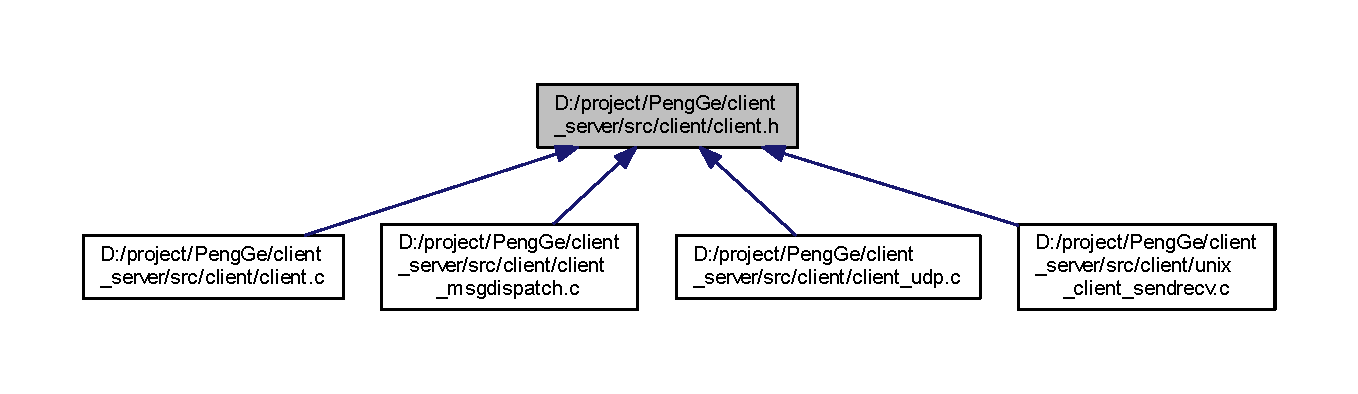
\includegraphics[width=350pt]{client_8h__dep__incl}
\end{center}
\end{figure}
\subsection*{Classes}
\begin{DoxyCompactItemize}
\item 
struct \hyperlink{structcsclient}{csclient}
\begin{DoxyCompactList}\small\item\em struct csclient contains necessary members and functions for client operations. This struct object must be initialized (by calling csclient\+\_\+init) before any operations applied to it. \end{DoxyCompactList}\end{DoxyCompactItemize}
\subsection*{Functions}
\begin{DoxyCompactItemize}
\item 
void \hyperlink{client_8h_a5aa275fcd29cc40dc4e8b04aca4836a8}{csclient\+\_\+init} (struct \hyperlink{structcsclient}{csclient} $\ast$cli, int tcpudp)
\begin{DoxyCompactList}\small\item\em csclient\+\_\+init \end{DoxyCompactList}\item 
void \hyperlink{client_8h_ae3752395d79c6d9a2920d96c73eb81ed}{csclient\+\_\+clear} (struct \hyperlink{structcsclient}{csclient} $\ast$cli)
\begin{DoxyCompactList}\small\item\em csclient\+\_\+clear There may be some clear works after communication, such as free the memory. \end{DoxyCompactList}\item 
\hypertarget{client_8h_a20e5a0eb2e564b26d13f5ab34c1a5986}{}void {\bfseries csclient\+\_\+connect} (struct \hyperlink{structcsclient}{csclient} $\ast$cli, const struct sockaddr $\ast$servaddr, cssocklen\+\_\+t addrlen)\label{client_8h_a20e5a0eb2e564b26d13f5ab34c1a5986}

\item 
int \hyperlink{client_8h_aa263fe24e3c96c3a1b1b8c087eb518b7}{csclient\+\_\+print} (const struct \hyperlink{structcsclient}{csclient} $\ast$cli)
\begin{DoxyCompactList}\small\item\em csclient\+\_\+print csclient\+\_\+print will test and print client socket information. If test fail, process will clear the socket environmtn and exit. \end{DoxyCompactList}\item 
void \hyperlink{client_8h_a8be5e8ba05fdac392536b4bb22d8914b}{csclient\+\_\+udp} (struct \hyperlink{structcsclient}{csclient} $\ast$cli, F\+I\+L\+E $\ast$fp, const struct sockaddr $\ast$servaddr, cssocklen\+\_\+t addrlen)
\begin{DoxyCompactList}\small\item\em csclient\+\_\+udp This function process udp communication with server. This function call csclient\+\_\+udp\+\_\+once in a loop. \end{DoxyCompactList}\item 
void \hyperlink{client_8h_a571252c127c68c849fdf766d6cef63e2}{csclient\+\_\+udp\+\_\+once} (struct \hyperlink{structcsclient}{csclient} $\ast$cli, const struct sockaddr $\ast$servaddr, cssocklen\+\_\+t addrlen)
\begin{DoxyCompactList}\small\item\em csclient\+\_\+udp\+\_\+once This function process udp send\&recv one time. \end{DoxyCompactList}\item 
ssize\+\_\+t \hyperlink{client_8h_aeecc65b7dbf1e0ac8f806ba8f518dab9}{csclient\+\_\+sendrecv} (struct \hyperlink{structcsclient}{csclient} $\ast$cli, const struct sockaddr $\ast$servaddr, cssocklen\+\_\+t addrlen)
\begin{DoxyCompactList}\small\item\em csclient\+\_\+sendrecv \end{DoxyCompactList}\item 
\hypertarget{client_8h_a4fb698628f5356d8926c28c83e17ea55}{}void \hyperlink{client_8h_a4fb698628f5356d8926c28c83e17ea55}{cssendrecv\+\_\+init} (void)\label{client_8h_a4fb698628f5356d8926c28c83e17ea55}

\begin{DoxyCompactList}\small\item\em cssendrecv\+\_\+init This function shoud better be called before the first call of csclient\+\_\+sendrecv. \end{DoxyCompactList}\item 
\hypertarget{client_8h_a5f15ec99768625f23952938f2619c020}{}void \hyperlink{client_8h_a5f15ec99768625f23952938f2619c020}{cssendrecv\+\_\+clear} (void)\label{client_8h_a5f15ec99768625f23952938f2619c020}

\begin{DoxyCompactList}\small\item\em cssendrecv\+\_\+clear This function must be called after client communication done. \end{DoxyCompactList}\end{DoxyCompactItemize}


\subsection{Detailed Description}
This file provide the basic helper funstion for client struct. 

\begin{DoxyAuthor}{Author}
cxl, \href{mailto:shuanglongchen@yeah.net}{\tt shuanglongchen@yeah.\+net} 
\end{DoxyAuthor}
\begin{DoxyVersion}{Version}
0.\+1 
\end{DoxyVersion}
\begin{DoxyDate}{Date}
2015-\/09-\/30 
\end{DoxyDate}
\begin{DoxyParagraph}{last modified}
Sat 2015-\/11-\/07 15\+:59\+:14 (+0800) 
\end{DoxyParagraph}


\subsection{Function Documentation}
\hypertarget{client_8h_ae3752395d79c6d9a2920d96c73eb81ed}{}\index{client.\+h@{client.\+h}!csclient\+\_\+clear@{csclient\+\_\+clear}}
\index{csclient\+\_\+clear@{csclient\+\_\+clear}!client.\+h@{client.\+h}}
\subsubsection[{csclient\+\_\+clear(struct csclient $\ast$cli)}]{\setlength{\rightskip}{0pt plus 5cm}void csclient\+\_\+clear (
\begin{DoxyParamCaption}
\item[{struct {\bf csclient} $\ast$}]{cli}
\end{DoxyParamCaption}
)}\label{client_8h_ae3752395d79c6d9a2920d96c73eb81ed}


csclient\+\_\+clear There may be some clear works after communication, such as free the memory. 


\begin{DoxyParams}{Parameters}
{\em cli} & \\
\hline
\end{DoxyParams}
\hypertarget{client_8h_a5aa275fcd29cc40dc4e8b04aca4836a8}{}\index{client.\+h@{client.\+h}!csclient\+\_\+init@{csclient\+\_\+init}}
\index{csclient\+\_\+init@{csclient\+\_\+init}!client.\+h@{client.\+h}}
\subsubsection[{csclient\+\_\+init(struct csclient $\ast$cli, int tcpudp)}]{\setlength{\rightskip}{0pt plus 5cm}void csclient\+\_\+init (
\begin{DoxyParamCaption}
\item[{struct {\bf csclient} $\ast$}]{cli, }
\item[{int}]{tcpudp}
\end{DoxyParamCaption}
)}\label{client_8h_a5aa275fcd29cc40dc4e8b04aca4836a8}


csclient\+\_\+init 


\begin{DoxyParams}{Parameters}
{\em cli} & \\
\hline
{\em tcpudp} & Tcp socket will be created if S\+O\+C\+K\+\_\+\+S\+T\+R\+E\+A\+M is set, upd socket will be created if S\+O\+C\+K\+\_\+\+D\+G\+R\+A\+M is set.\\
\hline
\end{DoxyParams}
\begin{DoxyNote}{Note}

\begin{DoxyEnumerate}
\item This function must be called after init\+\_\+sock\+\_\+environment being called.
\item Socket is set to be non-\/blocking socket by default. Call cssock\+\_\+block explicitly if you need the socket to be blocking.
\end{DoxyEnumerate}
\end{DoxyNote}
\begin{DoxySeeAlso}{See also}
\hyperlink{sock__wrap_8h_a60b0fd1896802faae9fd9dd341fadc54}{cssock\+\_\+block} \hyperlink{sock__wrap_8h_a842dda0d61b2e39aab64b40764adddd1}{cssock\+\_\+open} 
\end{DoxySeeAlso}


Here is the call graph for this function\+:
\nopagebreak
\begin{figure}[H]
\begin{center}
\leavevmode
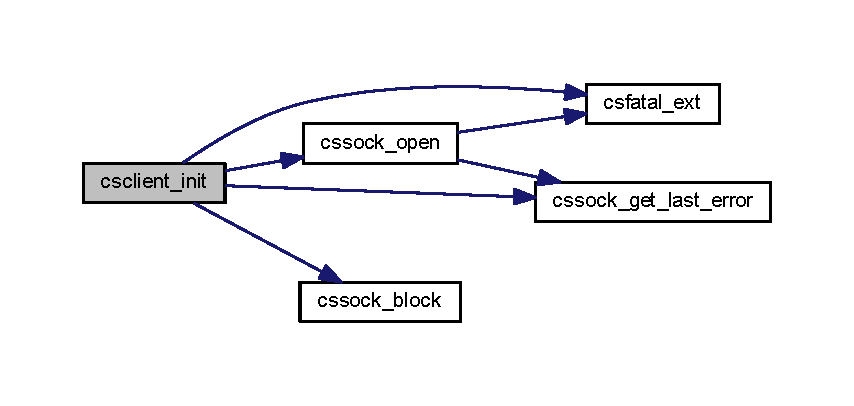
\includegraphics[width=350pt]{client_8h_a5aa275fcd29cc40dc4e8b04aca4836a8_cgraph}
\end{center}
\end{figure}


\hypertarget{client_8h_aa263fe24e3c96c3a1b1b8c087eb518b7}{}\index{client.\+h@{client.\+h}!csclient\+\_\+print@{csclient\+\_\+print}}
\index{csclient\+\_\+print@{csclient\+\_\+print}!client.\+h@{client.\+h}}
\subsubsection[{csclient\+\_\+print(const struct csclient $\ast$cli)}]{\setlength{\rightskip}{0pt plus 5cm}int csclient\+\_\+print (
\begin{DoxyParamCaption}
\item[{const struct {\bf csclient} $\ast$}]{cli}
\end{DoxyParamCaption}
)}\label{client_8h_aa263fe24e3c96c3a1b1b8c087eb518b7}


csclient\+\_\+print csclient\+\_\+print will test and print client socket information. If test fail, process will clear the socket environmtn and exit. 


\begin{DoxyParams}{Parameters}
{\em cli} & \\
\hline
\end{DoxyParams}
\begin{DoxyReturn}{Returns}

\begin{DoxyEnumerate}
\item -\/1, if socket is not a valid socket.
\item 0, if socket is connected.
\item 1, if socket is not connected.
\end{DoxyEnumerate}
\end{DoxyReturn}
\begin{DoxySeeAlso}{See also}
\hyperlink{sock__wrap_8h_a047455240499ada0472e5722cd50640b}{cssock\+\_\+print} 
\end{DoxySeeAlso}


Here is the call graph for this function\+:
\nopagebreak
\begin{figure}[H]
\begin{center}
\leavevmode
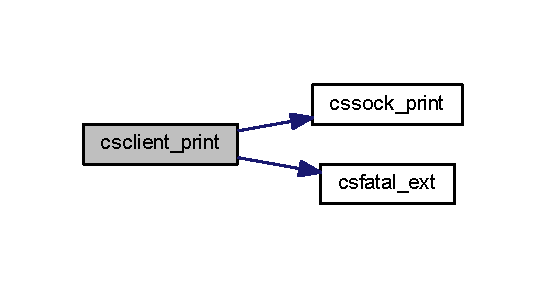
\includegraphics[width=262pt]{client_8h_aa263fe24e3c96c3a1b1b8c087eb518b7_cgraph}
\end{center}
\end{figure}


\hypertarget{client_8h_aeecc65b7dbf1e0ac8f806ba8f518dab9}{}\index{client.\+h@{client.\+h}!csclient\+\_\+sendrecv@{csclient\+\_\+sendrecv}}
\index{csclient\+\_\+sendrecv@{csclient\+\_\+sendrecv}!client.\+h@{client.\+h}}
\subsubsection[{csclient\+\_\+sendrecv(struct csclient $\ast$cli, const struct sockaddr $\ast$servaddr, cssocklen\+\_\+t addrlen)}]{\setlength{\rightskip}{0pt plus 5cm}ssize\+\_\+t csclient\+\_\+sendrecv (
\begin{DoxyParamCaption}
\item[{struct {\bf csclient} $\ast$}]{cli, }
\item[{const struct sockaddr $\ast$}]{servaddr, }
\item[{cssocklen\+\_\+t}]{addrlen}
\end{DoxyParamCaption}
)}\label{client_8h_aeecc65b7dbf1e0ac8f806ba8f518dab9}


csclient\+\_\+sendrecv 


\begin{DoxyParams}{Parameters}
{\em cli} & \\
\hline
{\em servaddr} & \\
\hline
{\em addrlen} & \\
\hline
\end{DoxyParams}
\begin{DoxyReturn}{Returns}

\begin{DoxyEnumerate}
\item number of bytes received.
\item -\/1, if timeout.
\item -\/2, if sendto error occurs.
\item -\/3, if recvfrom error occurs.
\end{DoxyEnumerate}
\end{DoxyReturn}
\begin{DoxySeeAlso}{See also}
\hyperlink{client_8h_a4fb698628f5356d8926c28c83e17ea55}{cssendrecv\+\_\+init} \hyperlink{client_8h_a5f15ec99768625f23952938f2619c020}{cssendrecv\+\_\+clear} 
\end{DoxySeeAlso}


Here is the call graph for this function\+:
\nopagebreak
\begin{figure}[H]
\begin{center}
\leavevmode
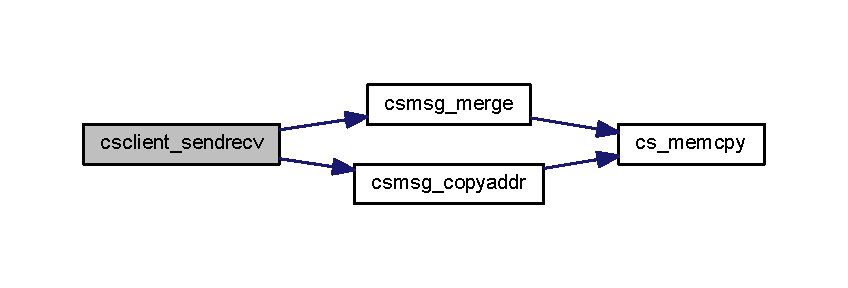
\includegraphics[width=350pt]{client_8h_aeecc65b7dbf1e0ac8f806ba8f518dab9_cgraph}
\end{center}
\end{figure}




Here is the caller graph for this function\+:
\nopagebreak
\begin{figure}[H]
\begin{center}
\leavevmode
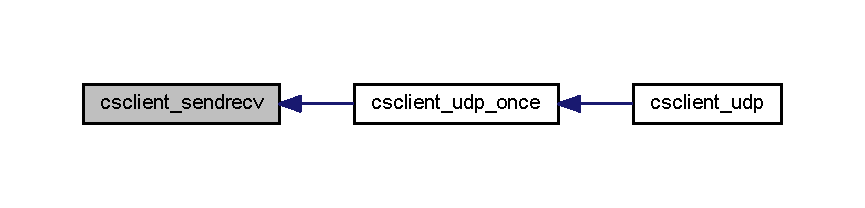
\includegraphics[width=350pt]{client_8h_aeecc65b7dbf1e0ac8f806ba8f518dab9_icgraph}
\end{center}
\end{figure}


\hypertarget{client_8h_a8be5e8ba05fdac392536b4bb22d8914b}{}\index{client.\+h@{client.\+h}!csclient\+\_\+udp@{csclient\+\_\+udp}}
\index{csclient\+\_\+udp@{csclient\+\_\+udp}!client.\+h@{client.\+h}}
\subsubsection[{csclient\+\_\+udp(struct csclient $\ast$cli, F\+I\+L\+E $\ast$fp, const struct sockaddr $\ast$servaddr, cssocklen\+\_\+t addrlen)}]{\setlength{\rightskip}{0pt plus 5cm}void csclient\+\_\+udp (
\begin{DoxyParamCaption}
\item[{struct {\bf csclient} $\ast$}]{cli, }
\item[{F\+I\+L\+E $\ast$}]{fp, }
\item[{const struct sockaddr $\ast$}]{servaddr, }
\item[{cssocklen\+\_\+t}]{addrlen}
\end{DoxyParamCaption}
)}\label{client_8h_a8be5e8ba05fdac392536b4bb22d8914b}


csclient\+\_\+udp This function process udp communication with server. This function call csclient\+\_\+udp\+\_\+once in a loop. 


\begin{DoxyParams}{Parameters}
{\em cli} & \\
\hline
{\em fp} & is the F\+I\+L\+E pointer where input data comes from. \\
\hline
{\em servaddr} & \\
\hline
{\em addrlen} & \\
\hline
\end{DoxyParams}
\begin{DoxySeeAlso}{See also}
\hyperlink{client_8h_a571252c127c68c849fdf766d6cef63e2}{csclient\+\_\+udp\+\_\+once} 
\end{DoxySeeAlso}


Here is the call graph for this function\+:
\nopagebreak
\begin{figure}[H]
\begin{center}
\leavevmode
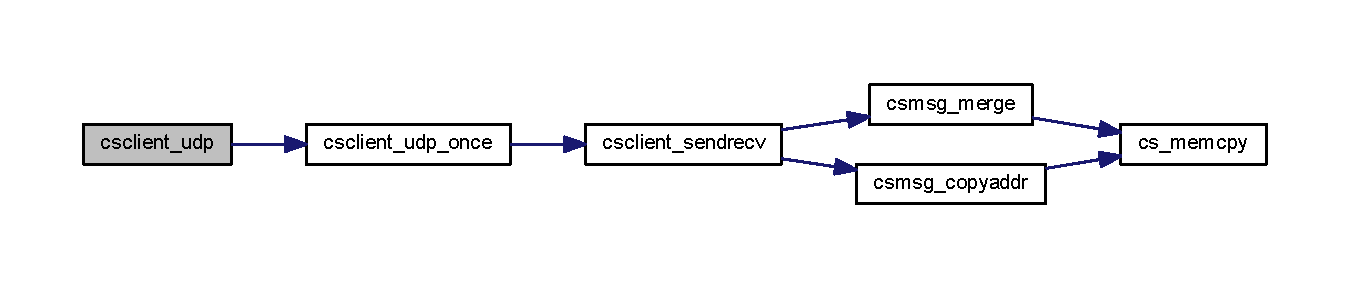
\includegraphics[width=350pt]{client_8h_a8be5e8ba05fdac392536b4bb22d8914b_cgraph}
\end{center}
\end{figure}


\hypertarget{client_8h_a571252c127c68c849fdf766d6cef63e2}{}\index{client.\+h@{client.\+h}!csclient\+\_\+udp\+\_\+once@{csclient\+\_\+udp\+\_\+once}}
\index{csclient\+\_\+udp\+\_\+once@{csclient\+\_\+udp\+\_\+once}!client.\+h@{client.\+h}}
\subsubsection[{csclient\+\_\+udp\+\_\+once(struct csclient $\ast$cli, const struct sockaddr $\ast$servaddr, cssocklen\+\_\+t addrlen)}]{\setlength{\rightskip}{0pt plus 5cm}void csclient\+\_\+udp\+\_\+once (
\begin{DoxyParamCaption}
\item[{struct {\bf csclient} $\ast$}]{cli, }
\item[{const struct sockaddr $\ast$}]{servaddr, }
\item[{cssocklen\+\_\+t}]{addrlen}
\end{DoxyParamCaption}
)}\label{client_8h_a571252c127c68c849fdf766d6cef63e2}


csclient\+\_\+udp\+\_\+once This function process udp send\&recv one time. 


\begin{DoxyParams}{Parameters}
{\em cli} & cli has already been filled with data(end with \textquotesingle{}\textbackslash{}0\textquotesingle{}) to send. \\
\hline
{\em servaddr} & \\
\hline
{\em addrlen} & \\
\hline
\end{DoxyParams}


Here is the call graph for this function\+:
\nopagebreak
\begin{figure}[H]
\begin{center}
\leavevmode
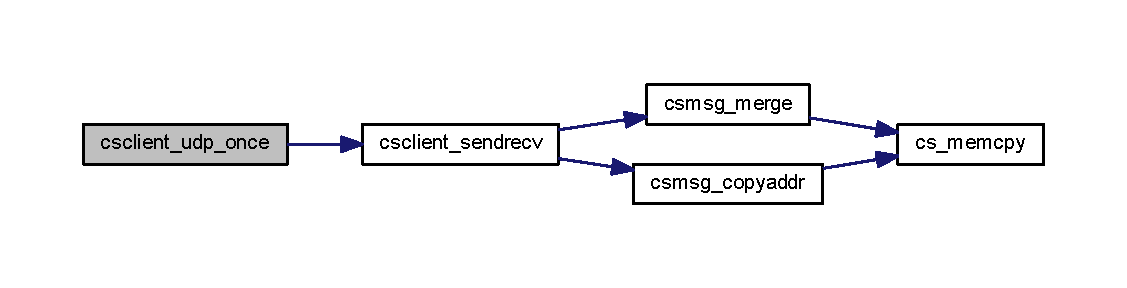
\includegraphics[width=350pt]{client_8h_a571252c127c68c849fdf766d6cef63e2_cgraph}
\end{center}
\end{figure}




Here is the caller graph for this function\+:
\nopagebreak
\begin{figure}[H]
\begin{center}
\leavevmode
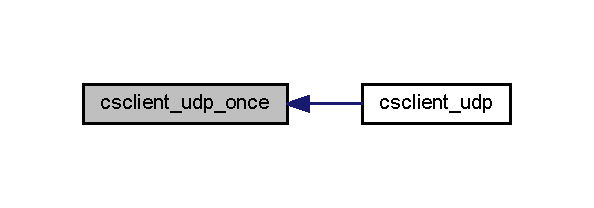
\includegraphics[width=285pt]{client_8h_a571252c127c68c849fdf766d6cef63e2_icgraph}
\end{center}
\end{figure}



\hypertarget{client__msgdispatch_8c}{}\section{D\+:/project/\+Peng\+Ge/client\+\_\+server/src/client/client\+\_\+msgdispatch.c File Reference}
\label{client__msgdispatch_8c}\index{D\+:/project/\+Peng\+Ge/client\+\_\+server/src/client/client\+\_\+msgdispatch.\+c@{D\+:/project/\+Peng\+Ge/client\+\_\+server/src/client/client\+\_\+msgdispatch.\+c}}
{\ttfamily \#include $<$sys/socket.\+h$>$}\\*
{\ttfamily \#include $<$netinet/in.\+h$>$}\\*
{\ttfamily \#include $<$stdio.\+h$>$}\\*
{\ttfamily \#include $<$string.\+h$>$}\\*
{\ttfamily \#include $<$stdint.\+h$>$}\\*
{\ttfamily \#include $<$semaphore.\+h$>$}\\*
{\ttfamily \#include \char`\"{}macros.\+h\char`\"{}}\\*
{\ttfamily \#include \char`\"{}lightthread.\+h\char`\"{}}\\*
{\ttfamily \#include \char`\"{}sock\+\_\+types.\+h\char`\"{}}\\*
{\ttfamily \#include \char`\"{}utility\+\_\+wrap.\+h\char`\"{}}\\*
{\ttfamily \#include \char`\"{}bufarray.\+h\char`\"{}}\\*
{\ttfamily \#include \char`\"{}msgpool.\+h\char`\"{}}\\*
{\ttfamily \#include \char`\"{}msgwrap.\+h\char`\"{}}\\*
{\ttfamily \#include \char`\"{}client.\+h\char`\"{}}\\*
Include dependency graph for client\+\_\+msgdispatch.\+c\+:
\nopagebreak
\begin{figure}[H]
\begin{center}
\leavevmode
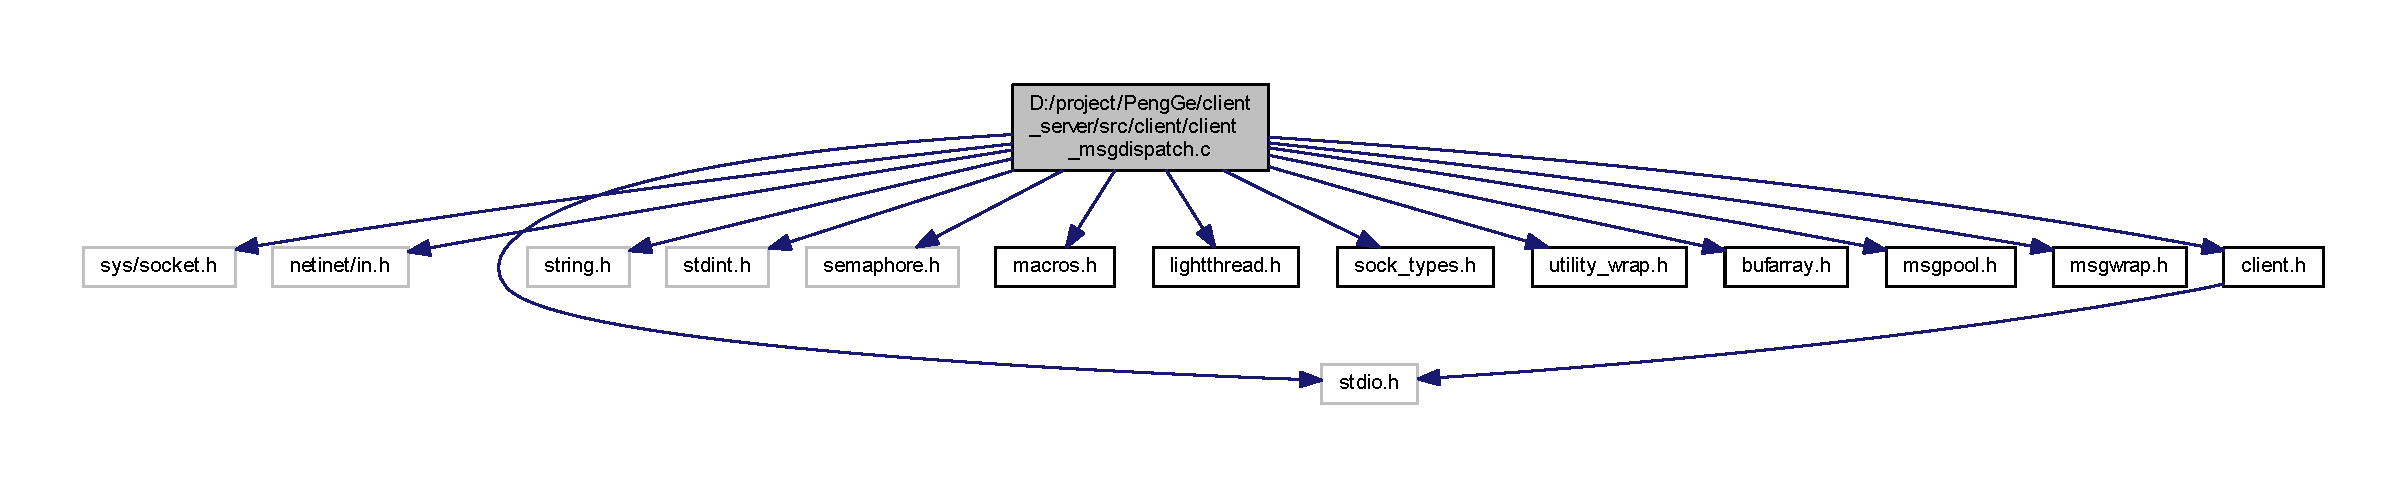
\includegraphics[width=350pt]{client__msgdispatch_8c__incl}
\end{center}
\end{figure}
\subsection*{Functions}
\begin{DoxyCompactItemize}
\item 
\hypertarget{client__msgdispatch_8c_ad3620cc2d153a5296c3f2da58d2babb4}{}void {\bfseries csclient\+\_\+process\+\_\+msg} (char $\ast$inmsg, char $\ast$outmsg, int $\ast$outmsglen, void $\ast$clidata)\label{client__msgdispatch_8c_ad3620cc2d153a5296c3f2da58d2babb4}

\end{DoxyCompactItemize}
\subsection*{Variables}
\begin{DoxyCompactItemize}
\item 
\hypertarget{client__msgdispatch_8c_a4520db064bea79e42630a63a529a450c}{}const char $\ast$ {\bfseries g\+\_\+loginmsg\+\_\+header}\label{client__msgdispatch_8c_a4520db064bea79e42630a63a529a450c}

\item 
\hypertarget{client__msgdispatch_8c_a928b0038fafc338c8cb7d6bd23764607}{}const char $\ast$ {\bfseries g\+\_\+logoutmsg\+\_\+header}\label{client__msgdispatch_8c_a928b0038fafc338c8cb7d6bd23764607}

\item 
\hypertarget{client__msgdispatch_8c_a60cacc9239d0662a686899339cf5b127}{}const char $\ast$ {\bfseries g\+\_\+loginmsg\+\_\+\+S\+U\+C\+C\+E\+S\+S}\label{client__msgdispatch_8c_a60cacc9239d0662a686899339cf5b127}

\item 
\hypertarget{client__msgdispatch_8c_ab241e51fd6b4014566bd16db0e23de58}{}const char $\ast$ {\bfseries g\+\_\+loginmsg\+\_\+\+F\+A\+I\+L}\label{client__msgdispatch_8c_ab241e51fd6b4014566bd16db0e23de58}

\item 
\hypertarget{client__msgdispatch_8c_a533bdde78cc9c28ca1a7c9418177f6a7}{}const char {\bfseries g\+\_\+login\+\_\+delimiter}\label{client__msgdispatch_8c_a533bdde78cc9c28ca1a7c9418177f6a7}

\end{DoxyCompactItemize}


\subsection{Detailed Description}
\begin{DoxyAuthor}{Author}
cxl, \href{mailto:shuanglongchen@yeah.net}{\tt shuanglongchen@yeah.\+net} 
\end{DoxyAuthor}
\begin{DoxyVersion}{Version}
0.\+1 
\end{DoxyVersion}
\begin{DoxyDate}{Date}
2015-\/11-\/07 
\end{DoxyDate}
\begin{DoxyParagraph}{last modified}
Sat 2015-\/11-\/07 14\+:46\+:59 (+0800) 
\end{DoxyParagraph}

\hypertarget{client__msgdispatch_8h}{}\section{D\+:/project/\+Peng\+Ge/client\+\_\+server/src/client/client\+\_\+msgdispatch.h File Reference}
\label{client__msgdispatch_8h}\index{D\+:/project/\+Peng\+Ge/client\+\_\+server/src/client/client\+\_\+msgdispatch.\+h@{D\+:/project/\+Peng\+Ge/client\+\_\+server/src/client/client\+\_\+msgdispatch.\+h}}


This file provides the process functions for message received from server. And the process function dispatches the message to corresponding handler.  


This graph shows which files directly or indirectly include this file\+:
\nopagebreak
\begin{figure}[H]
\begin{center}
\leavevmode
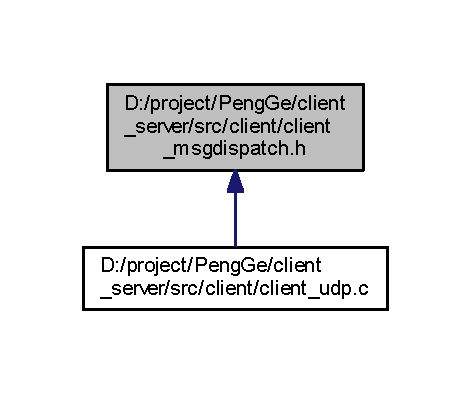
\includegraphics[width=226pt]{client__msgdispatch_8h__dep__incl}
\end{center}
\end{figure}
\subsection*{Functions}
\begin{DoxyCompactItemize}
\item 
\hypertarget{client__msgdispatch_8h_ad3620cc2d153a5296c3f2da58d2babb4}{}void {\bfseries csclient\+\_\+process\+\_\+msg} (char $\ast$inmsg, char $\ast$outmsg, int $\ast$outmsglen, void $\ast$clidata)\label{client__msgdispatch_8h_ad3620cc2d153a5296c3f2da58d2babb4}

\end{DoxyCompactItemize}


\subsection{Detailed Description}
This file provides the process functions for message received from server. And the process function dispatches the message to corresponding handler. 

\begin{DoxyAuthor}{Author}
cxl, \href{mailto:shuanglongchen@yeah.net}{\tt shuanglongchen@yeah.\+net} 
\end{DoxyAuthor}
\begin{DoxyVersion}{Version}
0.\+1 
\end{DoxyVersion}
\begin{DoxyDate}{Date}
2015-\/11-\/07 
\end{DoxyDate}
\begin{DoxyParagraph}{last modified}
Sat 2015-\/11-\/07 14\+:47\+:04 (+0800) 
\end{DoxyParagraph}

\hypertarget{client__udp_8c}{}\section{D\+:/project/\+Peng\+Ge/client\+\_\+server/src/client/client\+\_\+udp.c File Reference}
\label{client__udp_8c}\index{D\+:/project/\+Peng\+Ge/client\+\_\+server/src/client/client\+\_\+udp.\+c@{D\+:/project/\+Peng\+Ge/client\+\_\+server/src/client/client\+\_\+udp.\+c}}


This file prcess client udp message sendrecv. For now a lot config data is hard coded, reimplementation must be done when config parser complete.  


{\ttfamily \#include $<$sys/socket.\+h$>$}\\*
{\ttfamily \#include $<$netinet/in.\+h$>$}\\*
{\ttfamily \#include $<$pthread.\+h$>$}\\*
{\ttfamily \#include $<$unistd.\+h$>$}\\*
{\ttfamily \#include $<$assert.\+h$>$}\\*
{\ttfamily \#include $<$stdlib.\+h$>$}\\*
{\ttfamily \#include $<$stdio.\+h$>$}\\*
{\ttfamily \#include $<$stdint.\+h$>$}\\*
{\ttfamily \#include $<$string.\+h$>$}\\*
{\ttfamily \#include $<$semaphore.\+h$>$}\\*
{\ttfamily \#include \char`\"{}macros.\+h\char`\"{}}\\*
{\ttfamily \#include \char`\"{}bufarray.\+h\char`\"{}}\\*
{\ttfamily \#include \char`\"{}sock\+\_\+types.\+h\char`\"{}}\\*
{\ttfamily \#include \char`\"{}lightthread.\+h\char`\"{}}\\*
{\ttfamily \#include \char`\"{}utility\+\_\+wrap.\+h\char`\"{}}\\*
{\ttfamily \#include \char`\"{}msgpool.\+h\char`\"{}}\\*
{\ttfamily \#include \char`\"{}sock\+\_\+wrap.\+h\char`\"{}}\\*
{\ttfamily \#include \char`\"{}msgwrap.\+h\char`\"{}}\\*
{\ttfamily \#include \char`\"{}msgpool\+\_\+dispatch.\+h\char`\"{}}\\*
{\ttfamily \#include \char`\"{}client.\+h\char`\"{}}\\*
{\ttfamily \#include \char`\"{}client\+\_\+msgdispatch.\+h\char`\"{}}\\*
Include dependency graph for client\+\_\+udp.\+c\+:
\nopagebreak
\begin{figure}[H]
\begin{center}
\leavevmode
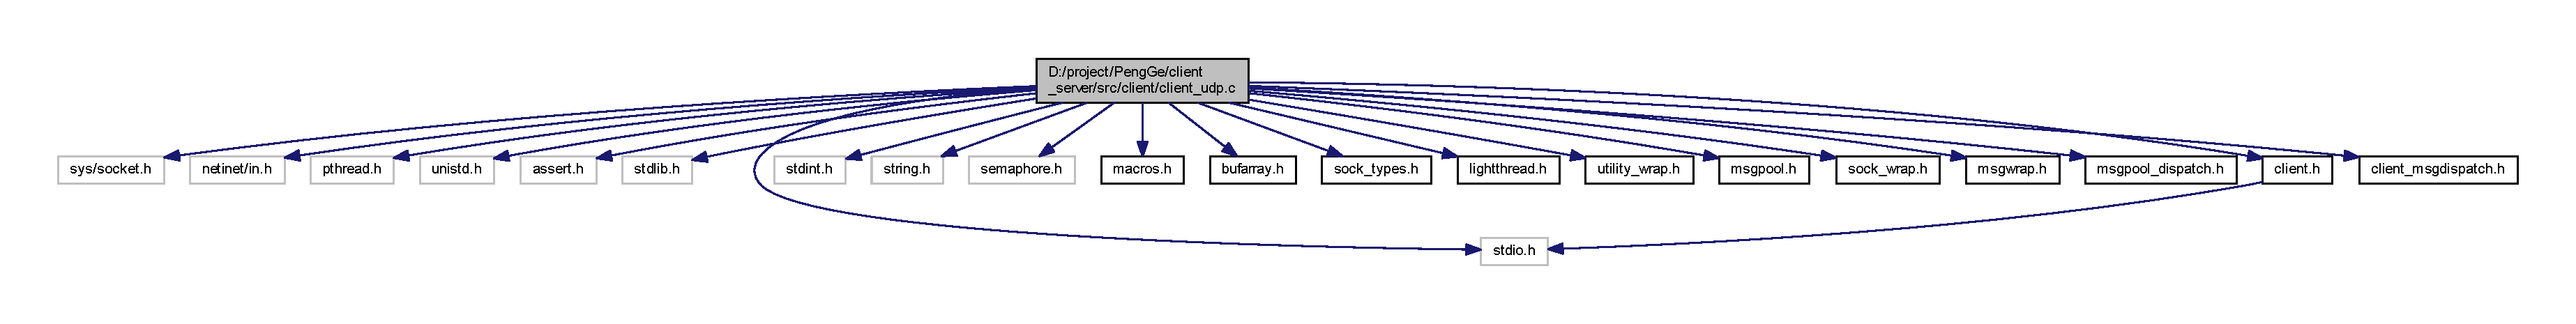
\includegraphics[width=350pt]{client__udp_8c__incl}
\end{center}
\end{figure}
\subsection*{Functions}
\begin{DoxyCompactItemize}
\item 
void \hyperlink{client__udp_8c_a8be5e8ba05fdac392536b4bb22d8914b}{csclient\+\_\+udp} (struct \hyperlink{structcsclient}{csclient} $\ast$cli, F\+I\+L\+E $\ast$fp, const struct sockaddr $\ast$servaddr, cssocklen\+\_\+t addrlen)
\begin{DoxyCompactList}\small\item\em csclient\+\_\+udp This function process udp communication with server. This function call csclient\+\_\+udp\+\_\+once in a loop. \end{DoxyCompactList}\item 
void \hyperlink{client__udp_8c_a571252c127c68c849fdf766d6cef63e2}{csclient\+\_\+udp\+\_\+once} (struct \hyperlink{structcsclient}{csclient} $\ast$cli, const struct sockaddr $\ast$servaddr, cssocklen\+\_\+t addrlen)
\begin{DoxyCompactList}\small\item\em csclient\+\_\+udp\+\_\+once This function process udp send\&recv one time. \end{DoxyCompactList}\end{DoxyCompactItemize}
\subsection*{Variables}
\begin{DoxyCompactItemize}
\item 
\hypertarget{client__udp_8c_a174a730c25e8784070b32a669e817448}{}const char $\ast$ {\bfseries g\+\_\+exit}\label{client__udp_8c_a174a730c25e8784070b32a669e817448}

\end{DoxyCompactItemize}


\subsection{Detailed Description}
This file prcess client udp message sendrecv. For now a lot config data is hard coded, reimplementation must be done when config parser complete. 

\begin{DoxyAuthor}{Author}
cxl, \href{mailto:shuanglongchen@yeah.net}{\tt shuanglongchen@yeah.\+net} 
\end{DoxyAuthor}
\begin{DoxyVersion}{Version}
0.\+1 
\end{DoxyVersion}
\begin{DoxyDate}{Date}
2015-\/11-\/07 
\end{DoxyDate}
\begin{DoxyParagraph}{last modified}
Sat 2015-\/11-\/07 15\+:57\+:32 (+0800) 
\end{DoxyParagraph}


\subsection{Function Documentation}
\hypertarget{client__udp_8c_a8be5e8ba05fdac392536b4bb22d8914b}{}\index{client\+\_\+udp.\+c@{client\+\_\+udp.\+c}!csclient\+\_\+udp@{csclient\+\_\+udp}}
\index{csclient\+\_\+udp@{csclient\+\_\+udp}!client\+\_\+udp.\+c@{client\+\_\+udp.\+c}}
\subsubsection[{csclient\+\_\+udp(struct csclient $\ast$cli, F\+I\+L\+E $\ast$fp, const struct sockaddr $\ast$servaddr, cssocklen\+\_\+t addrlen)}]{\setlength{\rightskip}{0pt plus 5cm}void csclient\+\_\+udp (
\begin{DoxyParamCaption}
\item[{struct {\bf csclient} $\ast$}]{cli, }
\item[{F\+I\+L\+E $\ast$}]{fp, }
\item[{const struct sockaddr $\ast$}]{servaddr, }
\item[{cssocklen\+\_\+t}]{addrlen}
\end{DoxyParamCaption}
)}\label{client__udp_8c_a8be5e8ba05fdac392536b4bb22d8914b}


csclient\+\_\+udp This function process udp communication with server. This function call csclient\+\_\+udp\+\_\+once in a loop. 


\begin{DoxyParams}{Parameters}
{\em cli} & \\
\hline
{\em fp} & is the F\+I\+L\+E pointer where input data comes from. \\
\hline
{\em servaddr} & \\
\hline
{\em addrlen} & \\
\hline
\end{DoxyParams}
\begin{DoxySeeAlso}{See also}
\hyperlink{client_8h_a571252c127c68c849fdf766d6cef63e2}{csclient\+\_\+udp\+\_\+once} 
\end{DoxySeeAlso}


Here is the call graph for this function\+:
\nopagebreak
\begin{figure}[H]
\begin{center}
\leavevmode
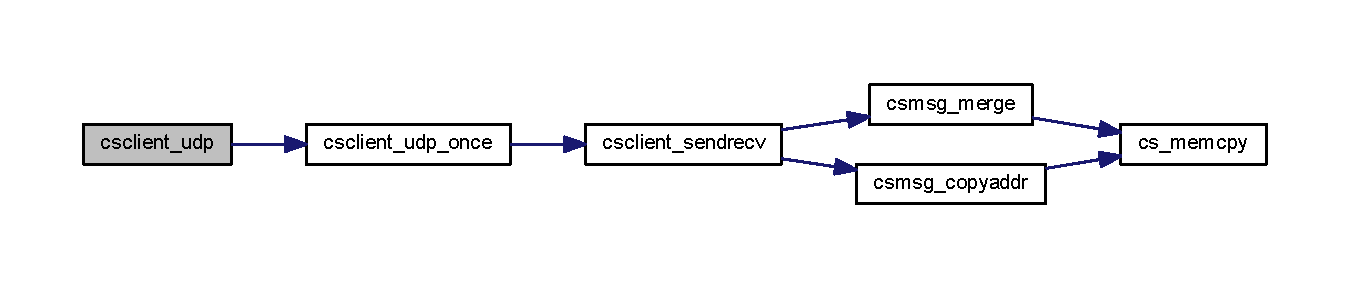
\includegraphics[width=350pt]{client__udp_8c_a8be5e8ba05fdac392536b4bb22d8914b_cgraph}
\end{center}
\end{figure}


\hypertarget{client__udp_8c_a571252c127c68c849fdf766d6cef63e2}{}\index{client\+\_\+udp.\+c@{client\+\_\+udp.\+c}!csclient\+\_\+udp\+\_\+once@{csclient\+\_\+udp\+\_\+once}}
\index{csclient\+\_\+udp\+\_\+once@{csclient\+\_\+udp\+\_\+once}!client\+\_\+udp.\+c@{client\+\_\+udp.\+c}}
\subsubsection[{csclient\+\_\+udp\+\_\+once(struct csclient $\ast$cli, const struct sockaddr $\ast$servaddr, cssocklen\+\_\+t addrlen)}]{\setlength{\rightskip}{0pt plus 5cm}void csclient\+\_\+udp\+\_\+once (
\begin{DoxyParamCaption}
\item[{struct {\bf csclient} $\ast$}]{cli, }
\item[{const struct sockaddr $\ast$}]{servaddr, }
\item[{cssocklen\+\_\+t}]{addrlen}
\end{DoxyParamCaption}
)}\label{client__udp_8c_a571252c127c68c849fdf766d6cef63e2}


csclient\+\_\+udp\+\_\+once This function process udp send\&recv one time. 


\begin{DoxyParams}{Parameters}
{\em cli} & cli has already been filled with data(end with \textquotesingle{}\textbackslash{}0\textquotesingle{}) to send. \\
\hline
{\em servaddr} & \\
\hline
{\em addrlen} & \\
\hline
\end{DoxyParams}


Here is the call graph for this function\+:
\nopagebreak
\begin{figure}[H]
\begin{center}
\leavevmode
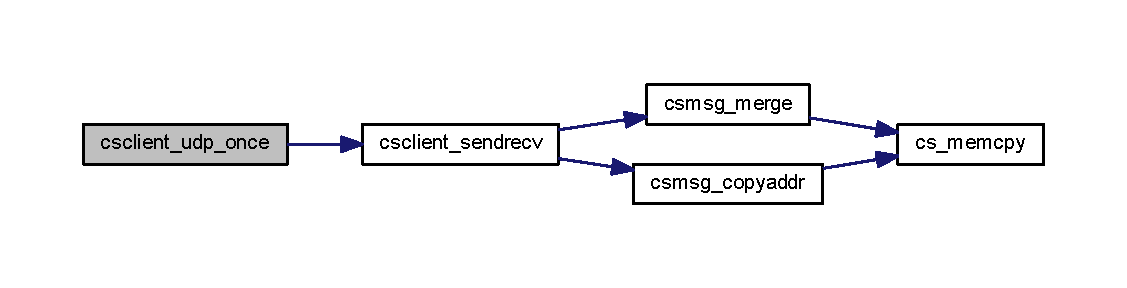
\includegraphics[width=350pt]{client__udp_8c_a571252c127c68c849fdf766d6cef63e2_cgraph}
\end{center}
\end{figure}




Here is the caller graph for this function\+:
\nopagebreak
\begin{figure}[H]
\begin{center}
\leavevmode
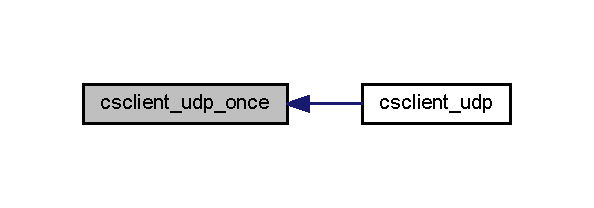
\includegraphics[width=285pt]{client__udp_8c_a571252c127c68c849fdf766d6cef63e2_icgraph}
\end{center}
\end{figure}



\hypertarget{unix__client__sendrecv_8c}{}\section{D\+:/project/\+Peng\+Ge/client\+\_\+server/src/client/unix\+\_\+client\+\_\+sendrecv.c File Reference}
\label{unix__client__sendrecv_8c}\index{D\+:/project/\+Peng\+Ge/client\+\_\+server/src/client/unix\+\_\+client\+\_\+sendrecv.\+c@{D\+:/project/\+Peng\+Ge/client\+\_\+server/src/client/unix\+\_\+client\+\_\+sendrecv.\+c}}


This file provide the linux version of client sendrecv.  


{\ttfamily \#include $<$stdio.\+h$>$}\\*
{\ttfamily \#include $<$string.\+h$>$}\\*
{\ttfamily \#include $<$unistd.\+h$>$}\\*
{\ttfamily \#include $<$errno.\+h$>$}\\*
{\ttfamily \#include $<$setjmp.\+h$>$}\\*
{\ttfamily \#include $<$signal.\+h$>$}\\*
{\ttfamily \#include $<$sys/socket.\+h$>$}\\*
{\ttfamily \#include $<$arpa/inet.\+h$>$}\\*
{\ttfamily \#include $<$pthread.\+h$>$}\\*
{\ttfamily \#include $<$semaphore.\+h$>$}\\*
{\ttfamily \#include \char`\"{}macros.\+h\char`\"{}}\\*
{\ttfamily \#include \char`\"{}unprtt.\+h\char`\"{}}\\*
{\ttfamily \#include \char`\"{}sock\+\_\+types.\+h\char`\"{}}\\*
{\ttfamily \#include \char`\"{}lightthread.\+h\char`\"{}}\\*
{\ttfamily \#include \char`\"{}sock\+\_\+wrap.\+h\char`\"{}}\\*
{\ttfamily \#include \char`\"{}bufarray.\+h\char`\"{}}\\*
{\ttfamily \#include \char`\"{}msgpool.\+h\char`\"{}}\\*
{\ttfamily \#include \char`\"{}msgwrap.\+h\char`\"{}}\\*
{\ttfamily \#include \char`\"{}utility\+\_\+wrap.\+h\char`\"{}}\\*
{\ttfamily \#include \char`\"{}client.\+h\char`\"{}}\\*
Include dependency graph for unix\+\_\+client\+\_\+sendrecv.\+c\+:
\nopagebreak
\begin{figure}[H]
\begin{center}
\leavevmode
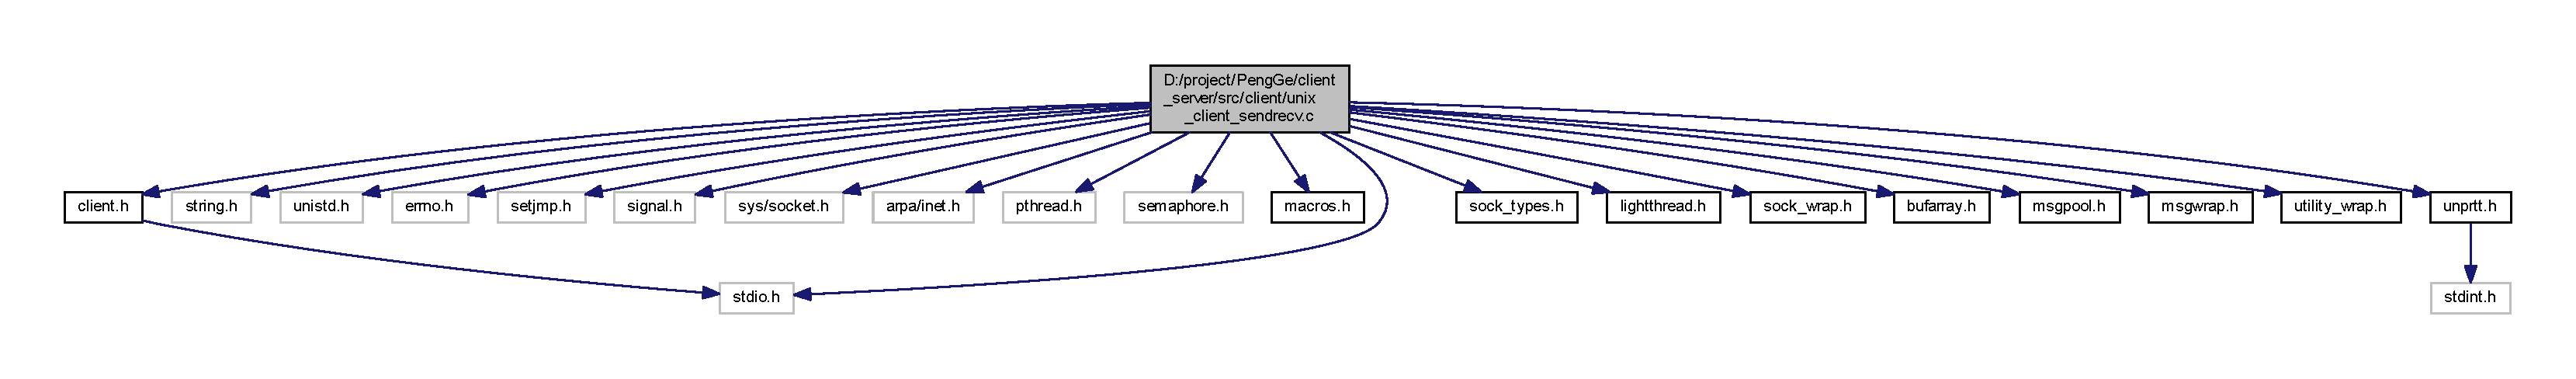
\includegraphics[width=350pt]{unix__client__sendrecv_8c__incl}
\end{center}
\end{figure}
\subsection*{Functions}
\begin{DoxyCompactItemize}
\item 
ssize\+\_\+t \hyperlink{unix__client__sendrecv_8c_aeecc65b7dbf1e0ac8f806ba8f518dab9}{csclient\+\_\+sendrecv} (struct \hyperlink{structcsclient}{csclient} $\ast$cli, const struct sockaddr $\ast$servaddr, cssocklen\+\_\+t addrlen)
\begin{DoxyCompactList}\small\item\em csclient\+\_\+sendrecv \end{DoxyCompactList}\item 
\hypertarget{unix__client__sendrecv_8c_a4fb698628f5356d8926c28c83e17ea55}{}void \hyperlink{unix__client__sendrecv_8c_a4fb698628f5356d8926c28c83e17ea55}{cssendrecv\+\_\+init} (void)\label{unix__client__sendrecv_8c_a4fb698628f5356d8926c28c83e17ea55}

\begin{DoxyCompactList}\small\item\em cssendrecv\+\_\+init This function shoud better be called before the first call of csclient\+\_\+sendrecv. \end{DoxyCompactList}\item 
\hypertarget{unix__client__sendrecv_8c_a5f15ec99768625f23952938f2619c020}{}void \hyperlink{unix__client__sendrecv_8c_a5f15ec99768625f23952938f2619c020}{cssendrecv\+\_\+clear} (void)\label{unix__client__sendrecv_8c_a5f15ec99768625f23952938f2619c020}

\begin{DoxyCompactList}\small\item\em cssendrecv\+\_\+clear This function must be called after client communication done. \end{DoxyCompactList}\end{DoxyCompactItemize}


\subsection{Detailed Description}
This file provide the linux version of client sendrecv. 

\begin{DoxyAuthor}{Author}
cxl, \href{mailto:shuanglongchen@yeah.net}{\tt shuanglongchen@yeah.\+net} 
\end{DoxyAuthor}
\begin{DoxyVersion}{Version}
0.\+1 
\end{DoxyVersion}
\begin{DoxyDate}{Date}
2015-\/10-\/31 
\end{DoxyDate}
\begin{DoxyParagraph}{last modified}
周五 2015-\/11-\/06 12\+:15\+:06 中国标准时间 
\end{DoxyParagraph}


\subsection{Function Documentation}
\hypertarget{unix__client__sendrecv_8c_aeecc65b7dbf1e0ac8f806ba8f518dab9}{}\index{unix\+\_\+client\+\_\+sendrecv.\+c@{unix\+\_\+client\+\_\+sendrecv.\+c}!csclient\+\_\+sendrecv@{csclient\+\_\+sendrecv}}
\index{csclient\+\_\+sendrecv@{csclient\+\_\+sendrecv}!unix\+\_\+client\+\_\+sendrecv.\+c@{unix\+\_\+client\+\_\+sendrecv.\+c}}
\subsubsection[{csclient\+\_\+sendrecv(struct csclient $\ast$cli, const struct sockaddr $\ast$servaddr, cssocklen\+\_\+t addrlen)}]{\setlength{\rightskip}{0pt plus 5cm}ssize\+\_\+t csclient\+\_\+sendrecv (
\begin{DoxyParamCaption}
\item[{struct {\bf csclient} $\ast$}]{cli, }
\item[{const struct sockaddr $\ast$}]{servaddr, }
\item[{cssocklen\+\_\+t}]{addrlen}
\end{DoxyParamCaption}
)}\label{unix__client__sendrecv_8c_aeecc65b7dbf1e0ac8f806ba8f518dab9}


csclient\+\_\+sendrecv 


\begin{DoxyParams}{Parameters}
{\em cli} & \\
\hline
{\em servaddr} & \\
\hline
{\em addrlen} & \\
\hline
\end{DoxyParams}
\begin{DoxyReturn}{Returns}

\begin{DoxyEnumerate}
\item number of bytes received.
\item -\/1, if timeout.
\item -\/2, if sendto error occurs.
\item -\/3, if recvfrom error occurs.
\end{DoxyEnumerate}
\end{DoxyReturn}
\begin{DoxySeeAlso}{See also}
\hyperlink{client_8h_a4fb698628f5356d8926c28c83e17ea55}{cssendrecv\+\_\+init} \hyperlink{client_8h_a5f15ec99768625f23952938f2619c020}{cssendrecv\+\_\+clear} 
\end{DoxySeeAlso}


Here is the call graph for this function\+:
\nopagebreak
\begin{figure}[H]
\begin{center}
\leavevmode
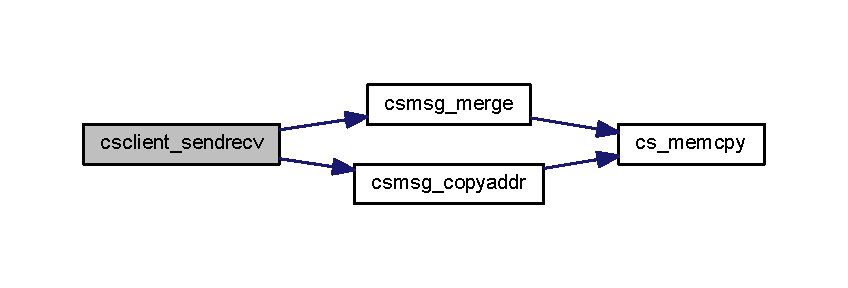
\includegraphics[width=350pt]{unix__client__sendrecv_8c_aeecc65b7dbf1e0ac8f806ba8f518dab9_cgraph}
\end{center}
\end{figure}




Here is the caller graph for this function\+:
\nopagebreak
\begin{figure}[H]
\begin{center}
\leavevmode
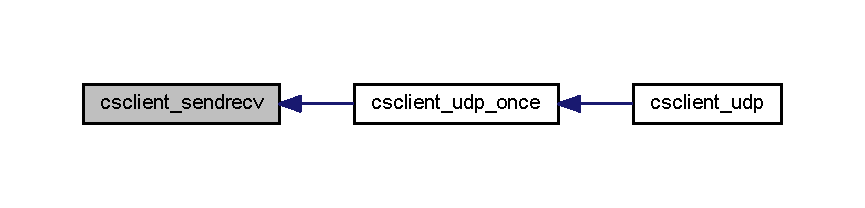
\includegraphics[width=350pt]{unix__client__sendrecv_8c_aeecc65b7dbf1e0ac8f806ba8f518dab9_icgraph}
\end{center}
\end{figure}



\hypertarget{bufarray_8c}{}\section{D\+:/project/\+Peng\+Ge/client\+\_\+server/src/common/bufarray.c File Reference}
\label{bufarray_8c}\index{D\+:/project/\+Peng\+Ge/client\+\_\+server/src/common/bufarray.\+c@{D\+:/project/\+Peng\+Ge/client\+\_\+server/src/common/bufarray.\+c}}


0.\+1  


{\ttfamily \#include $<$malloc.\+h$>$}\\*
{\ttfamily \#include $<$string.\+h$>$}\\*
{\ttfamily \#include $<$stdio.\+h$>$}\\*
{\ttfamily \#include \char`\"{}bufarray.\+h\char`\"{}}\\*
{\ttfamily \#include \char`\"{}macros.\+h\char`\"{}}\\*
Include dependency graph for bufarray.\+c\+:
\nopagebreak
\begin{figure}[H]
\begin{center}
\leavevmode
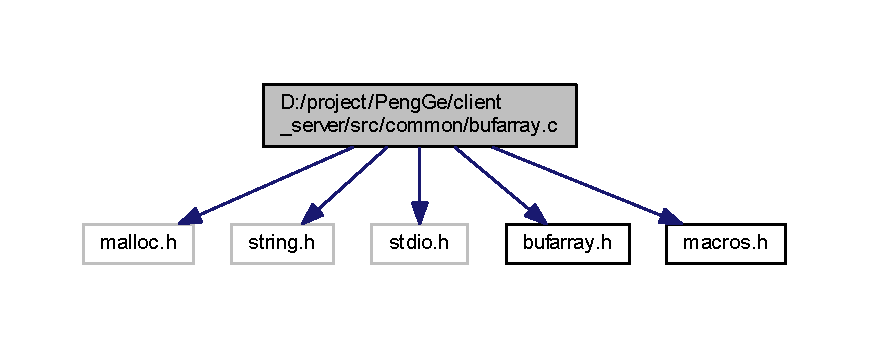
\includegraphics[width=350pt]{bufarray_8c__incl}
\end{center}
\end{figure}
\subsection*{Functions}
\begin{DoxyCompactItemize}
\item 
void \hyperlink{bufarray_8c_ad78700c530a64f81391a2639952d85c6}{init\+\_\+buf} (struct \hyperlink{structarray__buf}{array\+\_\+buf} $\ast$buf, int numitem, int lenitem, int nmalloc)
\begin{DoxyCompactList}\small\item\em init\+\_\+buf initialize struct array\+\_\+buf$\ast$. \end{DoxyCompactList}\end{DoxyCompactItemize}


\subsection{Detailed Description}
0.\+1 

\begin{DoxyAuthor}{Author}
cxl, \href{mailto:shuanglongchen@yeah.net}{\tt shuanglongchen@yeah.\+net} 
\end{DoxyAuthor}
\begin{DoxyVersion}{Version}
0.\+1 
\end{DoxyVersion}
\begin{DoxyDate}{Date}
2015-\/10-\/17 
\end{DoxyDate}


\subsection{Function Documentation}
\hypertarget{bufarray_8c_ad78700c530a64f81391a2639952d85c6}{}\index{bufarray.\+c@{bufarray.\+c}!init\+\_\+buf@{init\+\_\+buf}}
\index{init\+\_\+buf@{init\+\_\+buf}!bufarray.\+c@{bufarray.\+c}}
\subsubsection[{init\+\_\+buf(struct array\+\_\+buf $\ast$buf, int numitem, int lenitem, int nmalloc)}]{\setlength{\rightskip}{0pt plus 5cm}void init\+\_\+buf (
\begin{DoxyParamCaption}
\item[{struct {\bf array\+\_\+buf} $\ast$}]{buf, }
\item[{int}]{numitem, }
\item[{int}]{lenitem, }
\item[{int}]{nmalloc}
\end{DoxyParamCaption}
)}\label{bufarray_8c_ad78700c530a64f81391a2639952d85c6}


init\+\_\+buf initialize struct array\+\_\+buf$\ast$. 


\begin{DoxyParams}{Parameters}
{\em buf} & is the struct array\+\_\+buf$\ast$ to init. \\
\hline
{\em numitem} & is the number of items in struct \hyperlink{structarray__buf}{array\+\_\+buf}. \textquotesingle{}num\+\_\+item\textquotesingle{} will be set to the smallest number that fit\+: ((num\+\_\+item $>$= numitem) \&\& ((num\+\_\+item \% 4) == 0)) \\
\hline
{\em lenitem} & is the length of every item in struct \hyperlink{structarray__buf}{array\+\_\+buf}. \textquotesingle{}len\+\_\+item\textquotesingle{} will be set to the smallest number that fit\+: ((len\+\_\+item $>$= lenitem) \&\& ((len\+\_\+iem \% 512) == 0)) \\
\hline
{\em nmalloc} & is the number of item data to be malloc. This parameter will be change in the following principles in the function\+:
\begin{DoxyEnumerate}
\item if nmalloc is less than 0 or greater equal than \textquotesingle{}numitem\textquotesingle{}, nmalloc will be set to \textquotesingle{}numitem\textquotesingle{}.
\item otherwise nmalloc will be set to the smallest number that fit\+: ((nmalloc $>$= numitem) \&\& ((nmalloc \% 4) == 0)) 
\end{DoxyEnumerate}\\
\hline
\end{DoxyParams}

\hypertarget{bufarray_8h}{}\section{D\+:/project/\+Peng\+Ge/client\+\_\+server/src/common/bufarray.h File Reference}
\label{bufarray_8h}\index{D\+:/project/\+Peng\+Ge/client\+\_\+server/src/common/bufarray.\+h@{D\+:/project/\+Peng\+Ge/client\+\_\+server/src/common/bufarray.\+h}}


The basic buffer operations that implemented with circular queue.  


This graph shows which files directly or indirectly include this file\+:
\nopagebreak
\begin{figure}[H]
\begin{center}
\leavevmode
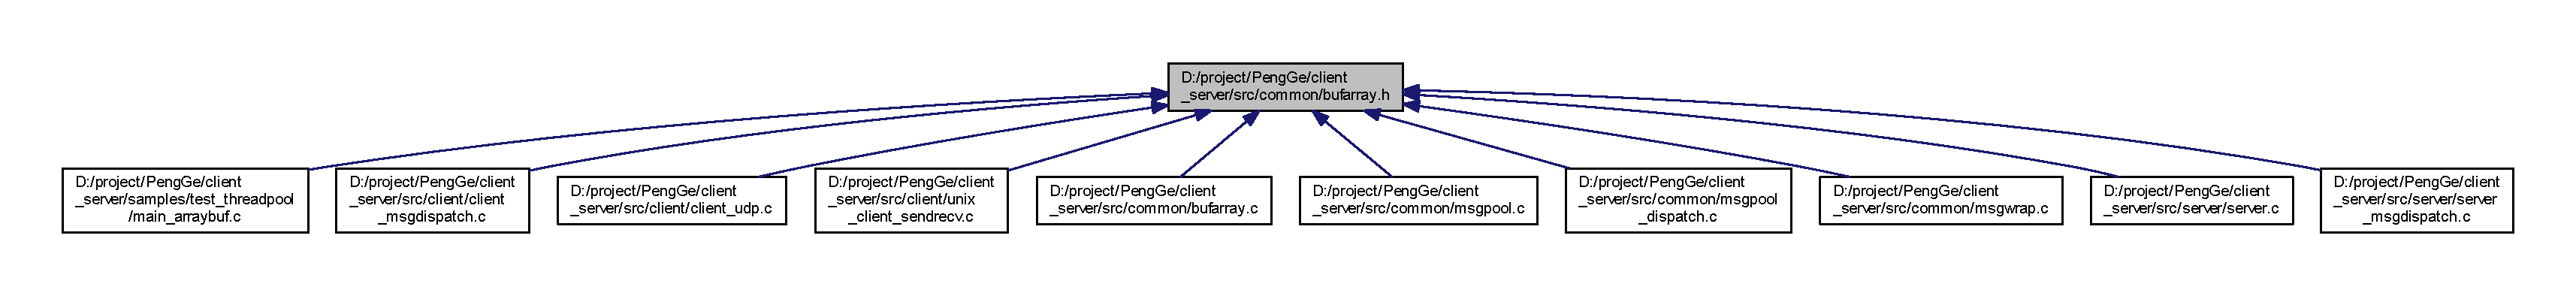
\includegraphics[width=350pt]{bufarray_8h__dep__incl}
\end{center}
\end{figure}
\subsection*{Classes}
\begin{DoxyCompactItemize}
\item 
struct \hyperlink{structarray__buf}{array\+\_\+buf}
\begin{DoxyCompactList}\small\item\em \hyperlink{structarray__buf}{array\+\_\+buf} is used to hold data. This struct works like circle queue(tail-\/in head-\/out). \end{DoxyCompactList}\end{DoxyCompactItemize}
\subsection*{Functions}
\begin{DoxyCompactItemize}
\item 
void \hyperlink{bufarray_8h_ad78700c530a64f81391a2639952d85c6}{init\+\_\+buf} (struct \hyperlink{structarray__buf}{array\+\_\+buf} $\ast$buf, int numitem, int lenitem, int nmalloc)
\begin{DoxyCompactList}\small\item\em init\+\_\+buf initialize struct array\+\_\+buf$\ast$. \end{DoxyCompactList}\end{DoxyCompactItemize}


\subsection{Detailed Description}
The basic buffer operations that implemented with circular queue. 

\begin{DoxyAuthor}{Author}
cxl, \href{mailto:shuanglongchen@yeah.net}{\tt shuanglongchen@yeah.\+net} 
\end{DoxyAuthor}
\begin{DoxyVersion}{Version}
0.\+1 
\end{DoxyVersion}
\begin{DoxyDate}{Date}
2015-\/10-\/17 
\end{DoxyDate}


\subsection{Function Documentation}
\hypertarget{bufarray_8h_ad78700c530a64f81391a2639952d85c6}{}\index{bufarray.\+h@{bufarray.\+h}!init\+\_\+buf@{init\+\_\+buf}}
\index{init\+\_\+buf@{init\+\_\+buf}!bufarray.\+h@{bufarray.\+h}}
\subsubsection[{init\+\_\+buf(struct array\+\_\+buf $\ast$buf, int numitem, int lenitem, int nmalloc)}]{\setlength{\rightskip}{0pt plus 5cm}void init\+\_\+buf (
\begin{DoxyParamCaption}
\item[{struct {\bf array\+\_\+buf} $\ast$}]{buf, }
\item[{int}]{numitem, }
\item[{int}]{lenitem, }
\item[{int}]{nmalloc}
\end{DoxyParamCaption}
)}\label{bufarray_8h_ad78700c530a64f81391a2639952d85c6}


init\+\_\+buf initialize struct array\+\_\+buf$\ast$. 


\begin{DoxyParams}{Parameters}
{\em buf} & is the struct array\+\_\+buf$\ast$ to init. \\
\hline
{\em numitem} & is the number of items in struct \hyperlink{structarray__buf}{array\+\_\+buf}. \textquotesingle{}num\+\_\+item\textquotesingle{} will be set to the smallest number that fit\+: ((num\+\_\+item $>$= numitem) \&\& ((num\+\_\+item \% 4) == 0)) \\
\hline
{\em lenitem} & is the length of every item in struct \hyperlink{structarray__buf}{array\+\_\+buf}. \textquotesingle{}len\+\_\+item\textquotesingle{} will be set to the smallest number that fit\+: ((len\+\_\+item $>$= lenitem) \&\& ((len\+\_\+iem \% 512) == 0)) \\
\hline
{\em nmalloc} & is the number of item data to be malloc. This parameter will be change in the following principles in the function\+:
\begin{DoxyEnumerate}
\item if nmalloc is less than 0 or greater equal than \textquotesingle{}numitem\textquotesingle{}, nmalloc will be set to \textquotesingle{}numitem\textquotesingle{}.
\item otherwise nmalloc will be set to the smallest number that fit\+: ((nmalloc $>$= numitem) \&\& ((nmalloc \% 4) == 0)) 
\end{DoxyEnumerate}\\
\hline
\end{DoxyParams}

\hypertarget{buflist_8c}{}\section{D\+:/project/\+Peng\+Ge/client\+\_\+server/src/common/buflist.c File Reference}
\label{buflist_8c}\index{D\+:/project/\+Peng\+Ge/client\+\_\+server/src/common/buflist.\+c@{D\+:/project/\+Peng\+Ge/client\+\_\+server/src/common/buflist.\+c}}
{\ttfamily \#include $<$malloc.\+h$>$}\\*
{\ttfamily \#include $<$stdio.\+h$>$}\\*
{\ttfamily \#include $<$assert.\+h$>$}\\*
{\ttfamily \#include \char`\"{}list.\+h\char`\"{}}\\*
{\ttfamily \#include \char`\"{}buflist.\+h\char`\"{}}\\*
{\ttfamily \#include \char`\"{}macros.\+h\char`\"{}}\\*
Include dependency graph for buflist.\+c\+:
\nopagebreak
\begin{figure}[H]
\begin{center}
\leavevmode
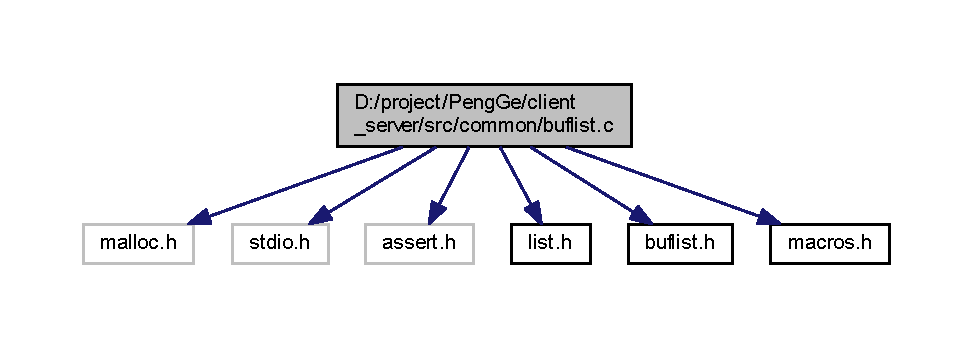
\includegraphics[width=350pt]{buflist_8c__incl}
\end{center}
\end{figure}
\subsection*{Functions}
\begin{DoxyCompactItemize}
\item 
\hypertarget{buflist_8c_af1ff98eb131849cf09a9de1f045ef866}{}void {\bfseries init\+\_\+buflist} (struct \hyperlink{structlist__head}{list\+\_\+head} $\ast$listhead, int listlen, int buflen)\label{buflist_8c_af1ff98eb131849cf09a9de1f045ef866}

\item 
\hypertarget{buflist_8c_a4b6dacf789afbaa3ba51f64693e6f0bd}{}void {\bfseries destroy\+\_\+buflist} (struct \hyperlink{structlist__head}{list\+\_\+head} $\ast$listhead)\label{buflist_8c_a4b6dacf789afbaa3ba51f64693e6f0bd}

\item 
\hypertarget{buflist_8c_a264cd5d0e04eca7b1c44e68fc451a307}{}struct \hyperlink{structbuf__node}{buf\+\_\+node} $\ast$ {\bfseries pullbuf} (struct \hyperlink{structlist__head}{list\+\_\+head} $\ast$listhead)\label{buflist_8c_a264cd5d0e04eca7b1c44e68fc451a307}

\item 
\hypertarget{buflist_8c_ac804f989f2fc7f77c47846f1244be44d}{}void {\bfseries pushbuf} (struct \hyperlink{structbuf__node}{buf\+\_\+node} $\ast$node, struct \hyperlink{structlist__head}{list\+\_\+head} $\ast$listhead)\label{buflist_8c_ac804f989f2fc7f77c47846f1244be44d}

\end{DoxyCompactItemize}


\subsection{Detailed Description}
\begin{DoxyAuthor}{Author}
cxl, \href{mailto:shuanglongchen@yeah.net}{\tt shuanglongchen@yeah.\+net} 
\end{DoxyAuthor}
\begin{DoxyVersion}{Version}
0.\+1 
\end{DoxyVersion}
\begin{DoxyDate}{Date}
2015-\/10-\/16 
\end{DoxyDate}

\hypertarget{buflist_8h}{}\section{D\+:/project/\+Peng\+Ge/client\+\_\+server/src/common/buflist.h File Reference}
\label{buflist_8h}\index{D\+:/project/\+Peng\+Ge/client\+\_\+server/src/common/buflist.\+h@{D\+:/project/\+Peng\+Ge/client\+\_\+server/src/common/buflist.\+h}}


The basic buffer operations that implemented with list.  


This graph shows which files directly or indirectly include this file\+:
\nopagebreak
\begin{figure}[H]
\begin{center}
\leavevmode
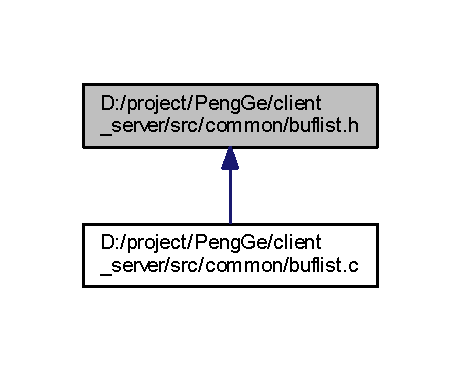
\includegraphics[width=221pt]{buflist_8h__dep__incl}
\end{center}
\end{figure}
\subsection*{Classes}
\begin{DoxyCompactItemize}
\item 
struct \hyperlink{structbuf__node}{buf\+\_\+node}
\end{DoxyCompactItemize}
\subsection*{Functions}
\begin{DoxyCompactItemize}
\item 
\hypertarget{buflist_8h_af1ff98eb131849cf09a9de1f045ef866}{}void {\bfseries init\+\_\+buflist} (struct \hyperlink{structlist__head}{list\+\_\+head} $\ast$listhead, int listlen, int buflen)\label{buflist_8h_af1ff98eb131849cf09a9de1f045ef866}

\item 
\hypertarget{buflist_8h_a4b6dacf789afbaa3ba51f64693e6f0bd}{}void {\bfseries destroy\+\_\+buflist} (struct \hyperlink{structlist__head}{list\+\_\+head} $\ast$listhead)\label{buflist_8h_a4b6dacf789afbaa3ba51f64693e6f0bd}

\item 
\hypertarget{buflist_8h_a264cd5d0e04eca7b1c44e68fc451a307}{}struct \hyperlink{structbuf__node}{buf\+\_\+node} $\ast$ {\bfseries pullbuf} (struct \hyperlink{structlist__head}{list\+\_\+head} $\ast$listhead)\label{buflist_8h_a264cd5d0e04eca7b1c44e68fc451a307}

\item 
\hypertarget{buflist_8h_ac804f989f2fc7f77c47846f1244be44d}{}void {\bfseries pushbuf} (struct \hyperlink{structbuf__node}{buf\+\_\+node} $\ast$node, struct \hyperlink{structlist__head}{list\+\_\+head} $\ast$listhead)\label{buflist_8h_ac804f989f2fc7f77c47846f1244be44d}

\end{DoxyCompactItemize}


\subsection{Detailed Description}
The basic buffer operations that implemented with list. 

\begin{DoxyAuthor}{Author}
cxl, \href{mailto:shuanglongchen@yeah.net}{\tt shuanglongchen@yeah.\+net} 
\end{DoxyAuthor}
\begin{DoxyVersion}{Version}
0.\+1 
\end{DoxyVersion}
\begin{DoxyDate}{Date}
2015-\/10-\/16 
\end{DoxyDate}

\hypertarget{error_8c}{}\section{D\+:/project/\+Peng\+Ge/client\+\_\+server/src/common/error.c File Reference}
\label{error_8c}\index{D\+:/project/\+Peng\+Ge/client\+\_\+server/src/common/error.\+c@{D\+:/project/\+Peng\+Ge/client\+\_\+server/src/common/error.\+c}}
{\ttfamily \#include $<$netinet/in.\+h$>$}\\*
{\ttfamily \#include $<$sys/socket.\+h$>$}\\*
{\ttfamily \#include $<$stdarg.\+h$>$}\\*
{\ttfamily \#include $<$stdio.\+h$>$}\\*
{\ttfamily \#include $<$stdlib.\+h$>$}\\*
{\ttfamily \#include $<$stdint.\+h$>$}\\*
{\ttfamily \#include \char`\"{}error.\+h\char`\"{}}\\*
{\ttfamily \#include \char`\"{}sock\+\_\+types.\+h\char`\"{}}\\*
{\ttfamily \#include \char`\"{}sock\+\_\+wrap.\+h\char`\"{}}\\*
Include dependency graph for error.\+c\+:
\nopagebreak
\begin{figure}[H]
\begin{center}
\leavevmode
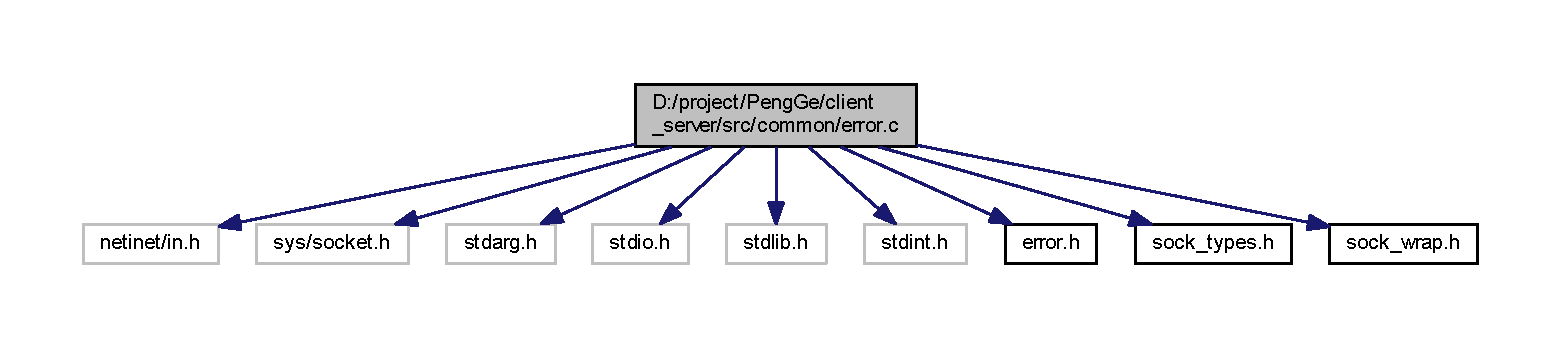
\includegraphics[width=350pt]{error_8c__incl}
\end{center}
\end{figure}
\subsection*{Functions}
\begin{DoxyCompactItemize}
\item 
\hypertarget{error_8c_aeed05a8aa6f9b854e305f1601893d1f5}{}void {\bfseries s\+\_\+cserr\+\_\+operation} (void $\ast$data, enum cserr\+\_\+op errop)\label{error_8c_aeed05a8aa6f9b854e305f1601893d1f5}

\item 
void \hyperlink{error_8c_a641ea5f626d774c1ae2eee06e8403e2a}{csfatal} (const char $\ast$format,...)
\begin{DoxyCompactList}\small\item\em csfatal Print csfatal error message and exit(0) \end{DoxyCompactList}\item 
void \hyperlink{error_8c_a6c106dc092c3356060fb1d64ac07a50d}{csfatal\+\_\+ext} (void $\ast$data, enum cserr\+\_\+op errop, const char $\ast$format,...)
\begin{DoxyCompactList}\small\item\em csfatal\+\_\+ext This function will print error message, clear socket environment and exit. If errop is cserr\+\_\+exit, exit($\ast$(cserr\+\_\+t$\ast$)data) will be called. if errop is cserr\+\_\+clear, ((cserr\+\_\+clear\+\_\+func)data)() will be called. \end{DoxyCompactList}\item 
void \hyperlink{error_8c_a373722baa5d63fdd892cf513205f2618}{cswarning} (const char $\ast$format,...)
\begin{DoxyCompactList}\small\item\em cswarning \end{DoxyCompactList}\item 
void \hyperlink{error_8c_ad92ec462d0139f28a5bb7d218f45b8a9}{cswarning\+\_\+ext} (void $\ast$data, enum cserr\+\_\+op errop, const char $\ast$format,...)
\begin{DoxyCompactList}\small\item\em cswarning\+\_\+ext \end{DoxyCompactList}\end{DoxyCompactItemize}


\subsection{Detailed Description}
\begin{DoxyAuthor}{Author}
cxl, \href{mailto:shuanglongchen@yeah.net}{\tt shuanglongchen@yeah.\+net} 
\end{DoxyAuthor}
\begin{DoxyVersion}{Version}
0.\+1 
\end{DoxyVersion}
\begin{DoxyDate}{Date}
2015-\/10-\/24 
\end{DoxyDate}
\begin{DoxyParagraph}{last modified}
Tue 2015-\/11-\/03 19\+:30\+:14 (+0800) 
\end{DoxyParagraph}


\subsection{Function Documentation}
\hypertarget{error_8c_a641ea5f626d774c1ae2eee06e8403e2a}{}\index{error.\+c@{error.\+c}!csfatal@{csfatal}}
\index{csfatal@{csfatal}!error.\+c@{error.\+c}}
\subsubsection[{csfatal(const char $\ast$format,...)}]{\setlength{\rightskip}{0pt plus 5cm}void csfatal (
\begin{DoxyParamCaption}
\item[{const char $\ast$}]{format, }
\item[{}]{...}
\end{DoxyParamCaption}
)}\label{error_8c_a641ea5f626d774c1ae2eee06e8403e2a}


csfatal Print csfatal error message and exit(0) 


\begin{DoxyParams}{Parameters}
{\em format} & \\
\hline
{\em ...} & \\
\hline
\end{DoxyParams}


Here is the call graph for this function\+:
\nopagebreak
\begin{figure}[H]
\begin{center}
\leavevmode
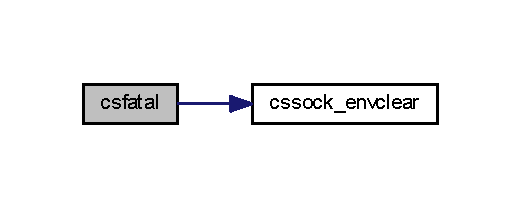
\includegraphics[width=250pt]{error_8c_a641ea5f626d774c1ae2eee06e8403e2a_cgraph}
\end{center}
\end{figure}




Here is the caller graph for this function\+:
\nopagebreak
\begin{figure}[H]
\begin{center}
\leavevmode
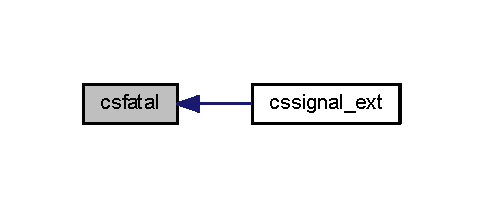
\includegraphics[width=232pt]{error_8c_a641ea5f626d774c1ae2eee06e8403e2a_icgraph}
\end{center}
\end{figure}


\hypertarget{error_8c_a6c106dc092c3356060fb1d64ac07a50d}{}\index{error.\+c@{error.\+c}!csfatal\+\_\+ext@{csfatal\+\_\+ext}}
\index{csfatal\+\_\+ext@{csfatal\+\_\+ext}!error.\+c@{error.\+c}}
\subsubsection[{csfatal\+\_\+ext(void $\ast$data, enum cserr\+\_\+op errop, const char $\ast$format,...)}]{\setlength{\rightskip}{0pt plus 5cm}void csfatal\+\_\+ext (
\begin{DoxyParamCaption}
\item[{void $\ast$}]{data, }
\item[{enum cserr\+\_\+op}]{errop, }
\item[{const char $\ast$}]{format, }
\item[{}]{...}
\end{DoxyParamCaption}
)}\label{error_8c_a6c106dc092c3356060fb1d64ac07a50d}


csfatal\+\_\+ext This function will print error message, clear socket environment and exit. If errop is cserr\+\_\+exit, exit($\ast$(cserr\+\_\+t$\ast$)data) will be called. if errop is cserr\+\_\+clear, ((cserr\+\_\+clear\+\_\+func)data)() will be called. 


\begin{DoxyParams}{Parameters}
{\em data} & \\
\hline
{\em errop} & \\
\hline
{\em format} & \\
\hline
{\em ...} & \\
\hline
\end{DoxyParams}


Here is the caller graph for this function\+:
\nopagebreak
\begin{figure}[H]
\begin{center}
\leavevmode
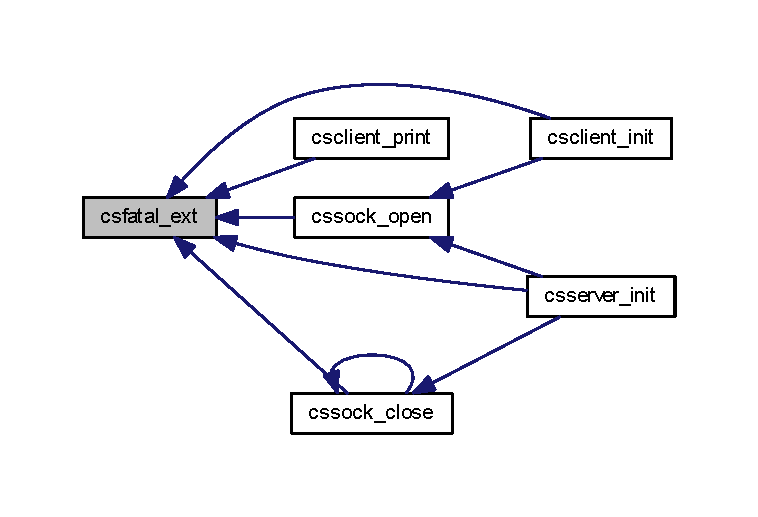
\includegraphics[width=350pt]{error_8c_a6c106dc092c3356060fb1d64ac07a50d_icgraph}
\end{center}
\end{figure}


\hypertarget{error_8c_a373722baa5d63fdd892cf513205f2618}{}\index{error.\+c@{error.\+c}!cswarning@{cswarning}}
\index{cswarning@{cswarning}!error.\+c@{error.\+c}}
\subsubsection[{cswarning(const char $\ast$format,...)}]{\setlength{\rightskip}{0pt plus 5cm}void cswarning (
\begin{DoxyParamCaption}
\item[{const char $\ast$}]{format, }
\item[{}]{...}
\end{DoxyParamCaption}
)}\label{error_8c_a373722baa5d63fdd892cf513205f2618}


cswarning 


\begin{DoxyParams}{Parameters}
{\em format} & \\
\hline
{\em ...} & \\
\hline
\end{DoxyParams}
\begin{DoxySeeAlso}{See also}
\hyperlink{error_8h_a641ea5f626d774c1ae2eee06e8403e2a}{csfatal} 
\end{DoxySeeAlso}
\hypertarget{error_8c_ad92ec462d0139f28a5bb7d218f45b8a9}{}\index{error.\+c@{error.\+c}!cswarning\+\_\+ext@{cswarning\+\_\+ext}}
\index{cswarning\+\_\+ext@{cswarning\+\_\+ext}!error.\+c@{error.\+c}}
\subsubsection[{cswarning\+\_\+ext(void $\ast$data, enum cserr\+\_\+op errop, const char $\ast$format,...)}]{\setlength{\rightskip}{0pt plus 5cm}void cswarning\+\_\+ext (
\begin{DoxyParamCaption}
\item[{void $\ast$}]{data, }
\item[{enum cserr\+\_\+op}]{errop, }
\item[{const char $\ast$}]{format, }
\item[{}]{...}
\end{DoxyParamCaption}
)}\label{error_8c_ad92ec462d0139f28a5bb7d218f45b8a9}


cswarning\+\_\+ext 


\begin{DoxyParams}{Parameters}
{\em data} & \\
\hline
{\em errop} & \\
\hline
{\em format} & \\
\hline
{\em ...} & \\
\hline
\end{DoxyParams}
\begin{DoxySeeAlso}{See also}
\hyperlink{error_8h_a6c106dc092c3356060fb1d64ac07a50d}{csfatal\+\_\+ext} 
\end{DoxySeeAlso}

\hypertarget{error_8h}{}\section{D\+:/project/\+Peng\+Ge/client\+\_\+server/src/common/error.h File Reference}
\label{error_8h}\index{D\+:/project/\+Peng\+Ge/client\+\_\+server/src/common/error.\+h@{D\+:/project/\+Peng\+Ge/client\+\_\+server/src/common/error.\+h}}


This file defines some crude error handlers.  


This graph shows which files directly or indirectly include this file\+:
\nopagebreak
\begin{figure}[H]
\begin{center}
\leavevmode
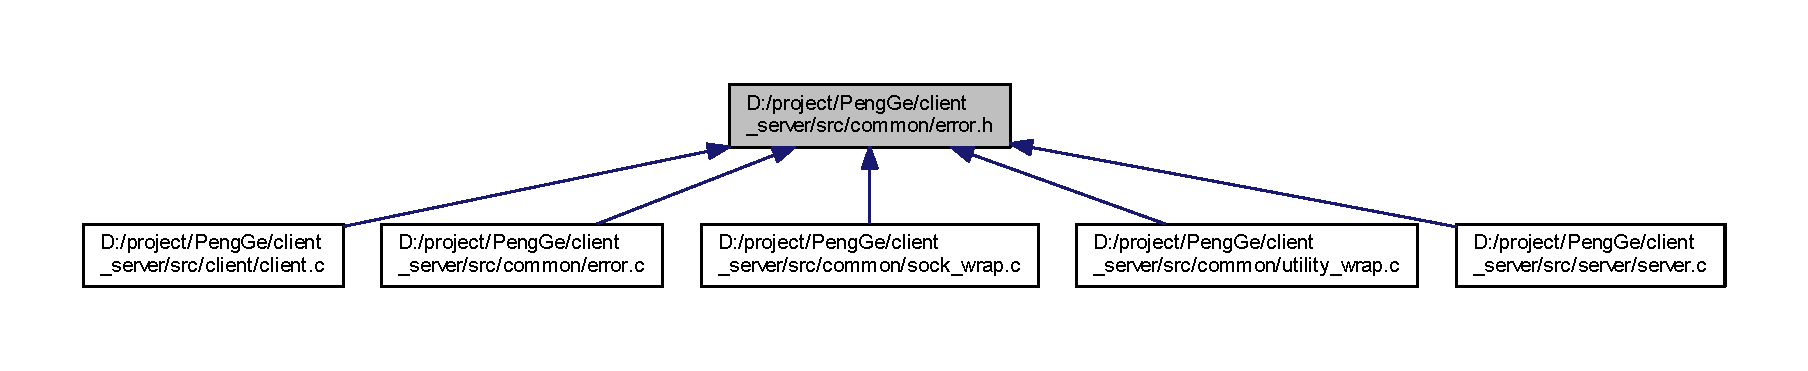
\includegraphics[width=350pt]{error_8h__dep__incl}
\end{center}
\end{figure}
\subsection*{Typedefs}
\begin{DoxyCompactItemize}
\item 
\hypertarget{error_8h_a95624e35bcd3bca0c67e5317c176aaa2}{}typedef size\+\_\+t {\bfseries cserr\+\_\+t}\label{error_8h_a95624e35bcd3bca0c67e5317c176aaa2}

\item 
\hypertarget{error_8h_ac497b149f0691140448cf70b79a47495}{}typedef void($\ast$ {\bfseries cserr\+\_\+clear\+\_\+func}) (void)\label{error_8h_ac497b149f0691140448cf70b79a47495}

\end{DoxyCompactItemize}
\subsection*{Enumerations}
\begin{DoxyCompactItemize}
\item 
\hypertarget{error_8h_a7f5f3f19273d7f61c3decb455da3a17e}{}enum {\bfseries cserr\+\_\+op} \{ {\bfseries cserr\+\_\+exit} = 0x0001, 
{\bfseries cserr\+\_\+clear} = 0x0002
 \}\label{error_8h_a7f5f3f19273d7f61c3decb455da3a17e}

\end{DoxyCompactItemize}
\subsection*{Functions}
\begin{DoxyCompactItemize}
\item 
void \hyperlink{error_8h_a641ea5f626d774c1ae2eee06e8403e2a}{csfatal} (const char $\ast$format,...)
\begin{DoxyCompactList}\small\item\em csfatal Print csfatal error message and exit(0) \end{DoxyCompactList}\item 
void \hyperlink{error_8h_a6c106dc092c3356060fb1d64ac07a50d}{csfatal\+\_\+ext} (void $\ast$data, enum cserr\+\_\+op errop, const char $\ast$format,...)
\begin{DoxyCompactList}\small\item\em csfatal\+\_\+ext This function will print error message, clear socket environment and exit. If errop is cserr\+\_\+exit, exit($\ast$(cserr\+\_\+t$\ast$)data) will be called. if errop is cserr\+\_\+clear, ((cserr\+\_\+clear\+\_\+func)data)() will be called. \end{DoxyCompactList}\item 
void \hyperlink{error_8h_a373722baa5d63fdd892cf513205f2618}{cswarning} (const char $\ast$format,...)
\begin{DoxyCompactList}\small\item\em cswarning \end{DoxyCompactList}\item 
void \hyperlink{error_8h_ad92ec462d0139f28a5bb7d218f45b8a9}{cswarning\+\_\+ext} (void $\ast$data, enum cserr\+\_\+op errop, const char $\ast$format,...)
\begin{DoxyCompactList}\small\item\em cswarning\+\_\+ext \end{DoxyCompactList}\end{DoxyCompactItemize}


\subsection{Detailed Description}
This file defines some crude error handlers. 

\begin{DoxyAuthor}{Author}
cxl, \href{mailto:shuanglongchen@yeah.net}{\tt shuanglongchen@yeah.\+net} 
\end{DoxyAuthor}
\begin{DoxyVersion}{Version}
0.\+1 
\end{DoxyVersion}
\begin{DoxyDate}{Date}
2015-\/10-\/24 
\end{DoxyDate}
\begin{DoxyParagraph}{last modified}
Tue 2015-\/11-\/03 19\+:24\+:51 (+0800) 
\end{DoxyParagraph}


\subsection{Function Documentation}
\hypertarget{error_8h_a641ea5f626d774c1ae2eee06e8403e2a}{}\index{error.\+h@{error.\+h}!csfatal@{csfatal}}
\index{csfatal@{csfatal}!error.\+h@{error.\+h}}
\subsubsection[{csfatal(const char $\ast$format,...)}]{\setlength{\rightskip}{0pt plus 5cm}void csfatal (
\begin{DoxyParamCaption}
\item[{const char $\ast$}]{format, }
\item[{}]{...}
\end{DoxyParamCaption}
)}\label{error_8h_a641ea5f626d774c1ae2eee06e8403e2a}


csfatal Print csfatal error message and exit(0) 


\begin{DoxyParams}{Parameters}
{\em format} & \\
\hline
{\em ...} & \\
\hline
\end{DoxyParams}


Here is the call graph for this function\+:
\nopagebreak
\begin{figure}[H]
\begin{center}
\leavevmode
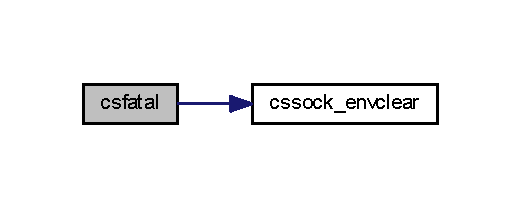
\includegraphics[width=250pt]{error_8h_a641ea5f626d774c1ae2eee06e8403e2a_cgraph}
\end{center}
\end{figure}




Here is the caller graph for this function\+:
\nopagebreak
\begin{figure}[H]
\begin{center}
\leavevmode
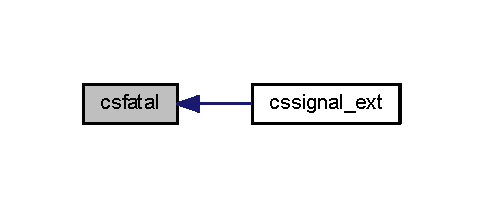
\includegraphics[width=232pt]{error_8h_a641ea5f626d774c1ae2eee06e8403e2a_icgraph}
\end{center}
\end{figure}


\hypertarget{error_8h_a6c106dc092c3356060fb1d64ac07a50d}{}\index{error.\+h@{error.\+h}!csfatal\+\_\+ext@{csfatal\+\_\+ext}}
\index{csfatal\+\_\+ext@{csfatal\+\_\+ext}!error.\+h@{error.\+h}}
\subsubsection[{csfatal\+\_\+ext(void $\ast$data, enum cserr\+\_\+op errop, const char $\ast$format,...)}]{\setlength{\rightskip}{0pt plus 5cm}void csfatal\+\_\+ext (
\begin{DoxyParamCaption}
\item[{void $\ast$}]{data, }
\item[{enum cserr\+\_\+op}]{errop, }
\item[{const char $\ast$}]{format, }
\item[{}]{...}
\end{DoxyParamCaption}
)}\label{error_8h_a6c106dc092c3356060fb1d64ac07a50d}


csfatal\+\_\+ext This function will print error message, clear socket environment and exit. If errop is cserr\+\_\+exit, exit($\ast$(cserr\+\_\+t$\ast$)data) will be called. if errop is cserr\+\_\+clear, ((cserr\+\_\+clear\+\_\+func)data)() will be called. 


\begin{DoxyParams}{Parameters}
{\em data} & \\
\hline
{\em errop} & \\
\hline
{\em format} & \\
\hline
{\em ...} & \\
\hline
\end{DoxyParams}


Here is the caller graph for this function\+:
\nopagebreak
\begin{figure}[H]
\begin{center}
\leavevmode
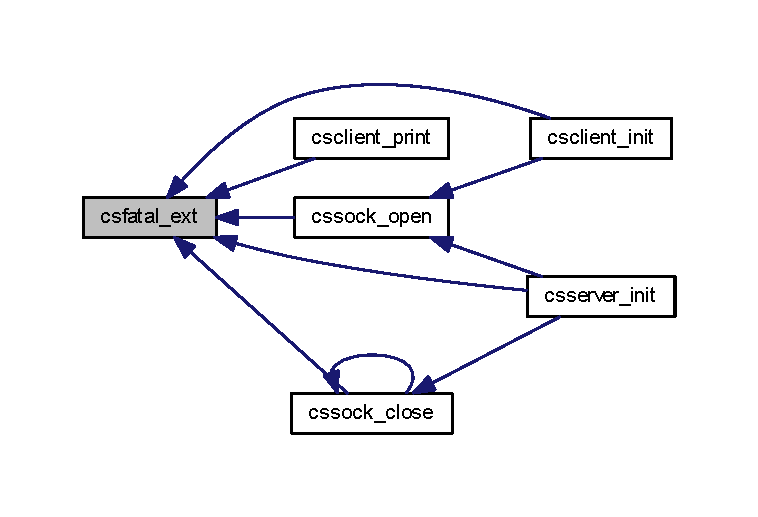
\includegraphics[width=350pt]{error_8h_a6c106dc092c3356060fb1d64ac07a50d_icgraph}
\end{center}
\end{figure}


\hypertarget{error_8h_a373722baa5d63fdd892cf513205f2618}{}\index{error.\+h@{error.\+h}!cswarning@{cswarning}}
\index{cswarning@{cswarning}!error.\+h@{error.\+h}}
\subsubsection[{cswarning(const char $\ast$format,...)}]{\setlength{\rightskip}{0pt plus 5cm}void cswarning (
\begin{DoxyParamCaption}
\item[{const char $\ast$}]{format, }
\item[{}]{...}
\end{DoxyParamCaption}
)}\label{error_8h_a373722baa5d63fdd892cf513205f2618}


cswarning 


\begin{DoxyParams}{Parameters}
{\em format} & \\
\hline
{\em ...} & \\
\hline
\end{DoxyParams}
\begin{DoxySeeAlso}{See also}
\hyperlink{error_8h_a641ea5f626d774c1ae2eee06e8403e2a}{csfatal} 
\end{DoxySeeAlso}
\hypertarget{error_8h_ad92ec462d0139f28a5bb7d218f45b8a9}{}\index{error.\+h@{error.\+h}!cswarning\+\_\+ext@{cswarning\+\_\+ext}}
\index{cswarning\+\_\+ext@{cswarning\+\_\+ext}!error.\+h@{error.\+h}}
\subsubsection[{cswarning\+\_\+ext(void $\ast$data, enum cserr\+\_\+op errop, const char $\ast$format,...)}]{\setlength{\rightskip}{0pt plus 5cm}void cswarning\+\_\+ext (
\begin{DoxyParamCaption}
\item[{void $\ast$}]{data, }
\item[{enum cserr\+\_\+op}]{errop, }
\item[{const char $\ast$}]{format, }
\item[{}]{...}
\end{DoxyParamCaption}
)}\label{error_8h_ad92ec462d0139f28a5bb7d218f45b8a9}


cswarning\+\_\+ext 


\begin{DoxyParams}{Parameters}
{\em data} & \\
\hline
{\em errop} & \\
\hline
{\em format} & \\
\hline
{\em ...} & \\
\hline
\end{DoxyParams}
\begin{DoxySeeAlso}{See also}
\hyperlink{error_8h_a6c106dc092c3356060fb1d64ac07a50d}{csfatal\+\_\+ext} 
\end{DoxySeeAlso}

\hypertarget{global_8c}{}\section{D\+:/project/\+Peng\+Ge/client\+\_\+server/src/common/global.c File Reference}
\label{global_8c}\index{D\+:/project/\+Peng\+Ge/client\+\_\+server/src/common/global.\+c@{D\+:/project/\+Peng\+Ge/client\+\_\+server/src/common/global.\+c}}


This file contains the global raviables.  


\subsection*{Variables}
\begin{DoxyCompactItemize}
\item 
\hypertarget{global_8c_a4520db064bea79e42630a63a529a450c}{}const char $\ast$ {\bfseries g\+\_\+loginmsg\+\_\+header} = \char`\"{}login\+: \char`\"{}\label{global_8c_a4520db064bea79e42630a63a529a450c}

\item 
\hypertarget{global_8c_a928b0038fafc338c8cb7d6bd23764607}{}const char $\ast$ {\bfseries g\+\_\+logoutmsg\+\_\+header} = \char`\"{}logout\char`\"{}\label{global_8c_a928b0038fafc338c8cb7d6bd23764607}

\item 
\hypertarget{global_8c_a60cacc9239d0662a686899339cf5b127}{}const char $\ast$ {\bfseries g\+\_\+loginmsg\+\_\+\+S\+U\+C\+C\+E\+S\+S} = \char`\"{}login\+\_\+success\char`\"{}\label{global_8c_a60cacc9239d0662a686899339cf5b127}

\item 
\hypertarget{global_8c_ab241e51fd6b4014566bd16db0e23de58}{}const char $\ast$ {\bfseries g\+\_\+loginmsg\+\_\+\+F\+A\+I\+L} = \char`\"{}login\+\_\+fail\char`\"{}\label{global_8c_ab241e51fd6b4014566bd16db0e23de58}

\item 
\hypertarget{global_8c_a533bdde78cc9c28ca1a7c9418177f6a7}{}const char {\bfseries g\+\_\+login\+\_\+delimiter} = \textquotesingle{} \textquotesingle{}\label{global_8c_a533bdde78cc9c28ca1a7c9418177f6a7}

\item 
\hypertarget{global_8c_a174a730c25e8784070b32a669e817448}{}const char $\ast$ {\bfseries g\+\_\+exit} = \char`\"{}exit\char`\"{}\label{global_8c_a174a730c25e8784070b32a669e817448}

\item 
\hypertarget{global_8c_a699d973470d18c0d8348fc3fd5f79266}{}const char $\ast$ {\bfseries g\+\_\+close} = \char`\"{}close\char`\"{}\label{global_8c_a699d973470d18c0d8348fc3fd5f79266}

\end{DoxyCompactItemize}


\subsection{Detailed Description}
This file contains the global raviables. 

\begin{DoxyAuthor}{Author}
cxl, \href{mailto:shuanglongchen@yeah.net}{\tt shuanglongchen@yeah.\+net} 
\end{DoxyAuthor}
\begin{DoxyVersion}{Version}
0.\+1 
\end{DoxyVersion}
\begin{DoxyDate}{Date}
2015-\/10-\/24 
\end{DoxyDate}
\begin{DoxyParagraph}{last modified}
Sat 2015-\/11-\/07 16\+:47\+:09 (+0800) 
\end{DoxyParagraph}

\hypertarget{lightthread_8c}{}\section{D\+:/project/\+Peng\+Ge/client\+\_\+server/src/common/lightthread.c File Reference}
\label{lightthread_8c}\index{D\+:/project/\+Peng\+Ge/client\+\_\+server/src/common/lightthread.\+c@{D\+:/project/\+Peng\+Ge/client\+\_\+server/src/common/lightthread.\+c}}
{\ttfamily \#include $<$errno.\+h$>$}\\*
{\ttfamily \#include $<$semaphore.\+h$>$}\\*
{\ttfamily \#include $<$pthread.\+h$>$}\\*
{\ttfamily \#include $<$unistd.\+h$>$}\\*
{\ttfamily \#include $<$sys/time.\+h$>$}\\*
{\ttfamily \#include $<$time.\+h$>$}\\*
{\ttfamily \#include $<$stdio.\+h$>$}\\*
{\ttfamily \#include $<$malloc.\+h$>$}\\*
{\ttfamily \#include $<$string.\+h$>$}\\*
{\ttfamily \#include \char`\"{}lightthread.\+h\char`\"{}}\\*
{\ttfamily \#include \char`\"{}macros.\+h\char`\"{}}\\*
{\ttfamily \#include \char`\"{}timespan.\+h\char`\"{}}\\*
Include dependency graph for lightthread.\+c\+:
\nopagebreak
\begin{figure}[H]
\begin{center}
\leavevmode
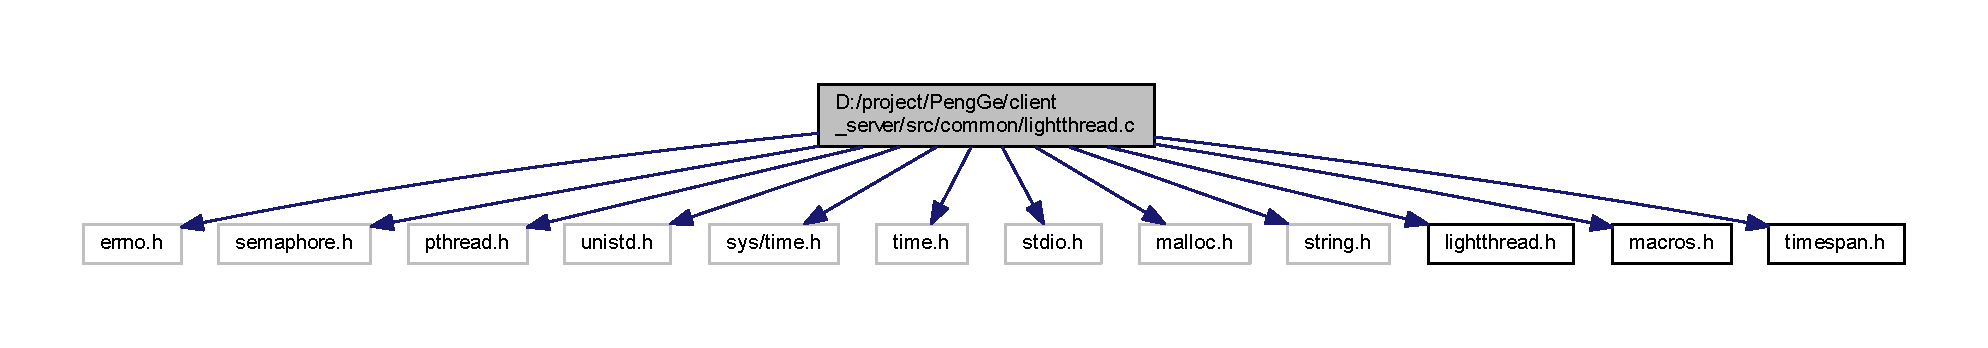
\includegraphics[width=350pt]{lightthread_8c__incl}
\end{center}
\end{figure}
\subsection*{Macros}
\begin{DoxyCompactItemize}
\item 
\hypertarget{lightthread_8c_a39e0a7f1b902181e5a84918c0acc9c76}{}\#define {\bfseries T\+H\+R\+E\+A\+D\+\_\+\+I\+D\+E\+L\+\_\+\+T\+I\+M\+E\+S\+L\+I\+C\+E\+\_\+\+M\+S}~20\label{lightthread_8c_a39e0a7f1b902181e5a84918c0acc9c76}

\end{DoxyCompactItemize}
\subsection*{Functions}
\begin{DoxyCompactItemize}
\item 
int \hyperlink{lightthread_8c_a56ae5a13616435e42ec013020a35cf59}{csthread\+\_\+create} (csthread\+\_\+proc\+\_\+t proc, void $\ast$pargs, csthread\+\_\+t $\ast$handle)
\begin{DoxyCompactList}\small\item\em The following block describe the windows thread functions. \end{DoxyCompactList}\item 
\hypertarget{lightthread_8c_a3f281b2855e0eb63360f12a1e745e088}{}void \hyperlink{lightthread_8c_a3f281b2855e0eb63360f12a1e745e088}{csthread\+\_\+exit} (void)\label{lightthread_8c_a3f281b2855e0eb63360f12a1e745e088}

\begin{DoxyCompactList}\small\item\em csthread\+\_\+exit \end{DoxyCompactList}\item 
void \hyperlink{lightthread_8c_a3be8a03a3c7ab0758d4dfe1c1a4939dd}{csthread\+\_\+wait\+\_\+terminate} (csthread\+\_\+t handle)
\begin{DoxyCompactList}\small\item\em csthread\+\_\+wait\+\_\+terminate \end{DoxyCompactList}\item 
void \hyperlink{lightthread_8c_a40598371a661aa6085b63b001f161a71}{csthread\+N\+\_\+wait\+\_\+terminate} (csthread\+\_\+t $\ast$handle, int count)
\begin{DoxyCompactList}\small\item\em csthread\+N\+\_\+wait\+\_\+terminate \end{DoxyCompactList}\item 
unsigned int \hyperlink{lightthread_8c_a16e901a07d7391faed2f6e41af336708}{csthread\+\_\+getpid} (void)
\begin{DoxyCompactList}\small\item\em csthread\+\_\+getpid \end{DoxyCompactList}\item 
void \hyperlink{lightthread_8c_a903de2b932fc9de89fd5952d217ddd15}{cssleep} (unsigned int msec)
\begin{DoxyCompactList}\small\item\em cssleep \end{DoxyCompactList}\item 
csmutex\+\_\+t \hyperlink{lightthread_8c_a5c3a7fb06b62b05a6dfa3359eb939655}{csmutex\+\_\+create} (void)
\begin{DoxyCompactList}\small\item\em csmutex\+\_\+create csmutex\+\_\+create will create the mutex and print error message if error occurs. \end{DoxyCompactList}\item 
void \hyperlink{lightthread_8c_aab46494a34bf1e3dbd157b8dd6ea04cb}{csmutex\+\_\+destroy} (csmutex\+\_\+t handle)
\begin{DoxyCompactList}\small\item\em csmutex\+\_\+destroy \end{DoxyCompactList}\item 
int \hyperlink{lightthread_8c_a78561b071805b213f88d0757b381aa92}{csmutex\+\_\+lock} (csmutex\+\_\+t handle)
\begin{DoxyCompactList}\small\item\em csmutex\+\_\+lock \end{DoxyCompactList}\item 
int \hyperlink{lightthread_8c_ad3a757691d8d36a947984c914a2fe5b3}{csmutex\+\_\+try\+\_\+lock} (csmutex\+\_\+t handle, unsigned int msec)
\begin{DoxyCompactList}\small\item\em csmutex\+\_\+try\+\_\+lock This function returns zero if a lock on the mutex object referenced by mutex is acquired. Otherwise, an error number is returned to indicate the error. \end{DoxyCompactList}\item 
void \hyperlink{lightthread_8c_abe0d10d1918d0b3fc8a9966e9710b632}{csmutex\+\_\+unlock} (csmutex\+\_\+t handle)
\begin{DoxyCompactList}\small\item\em csmutex\+\_\+unlock This function unlock the numtex. \end{DoxyCompactList}\item 
\hypertarget{lightthread_8c_a28c2302dea7cc0ccaa65453cc5dabead}{}int {\bfseries cssem\+\_\+create} (int value\+\_\+init, int value\+\_\+max, cssem\+\_\+t $\ast$handle)\label{lightthread_8c_a28c2302dea7cc0ccaa65453cc5dabead}

\end{DoxyCompactItemize}


\subsection{Detailed Description}
\begin{DoxyAuthor}{Author}
cxl, \href{mailto:shuanglongchen@yeah.net}{\tt shuanglongchen@yeah.\+net} 
\end{DoxyAuthor}
\begin{DoxyVersion}{Version}
0.\+1 
\end{DoxyVersion}
\begin{DoxyDate}{Date}
2015-\/10-\/26 
\end{DoxyDate}
\begin{DoxyParagraph}{last modified}
Wed 2015-\/11-\/04 17\+:29\+:07 (+0800) 
\end{DoxyParagraph}


\subsection{Function Documentation}
\hypertarget{lightthread_8c_a5c3a7fb06b62b05a6dfa3359eb939655}{}\index{lightthread.\+c@{lightthread.\+c}!csmutex\+\_\+create@{csmutex\+\_\+create}}
\index{csmutex\+\_\+create@{csmutex\+\_\+create}!lightthread.\+c@{lightthread.\+c}}
\subsubsection[{csmutex\+\_\+create(void)}]{\setlength{\rightskip}{0pt plus 5cm}csmutex\+\_\+t csmutex\+\_\+create (
\begin{DoxyParamCaption}
\item[{void}]{}
\end{DoxyParamCaption}
)}\label{lightthread_8c_a5c3a7fb06b62b05a6dfa3359eb939655}


csmutex\+\_\+create csmutex\+\_\+create will create the mutex and print error message if error occurs. 

\begin{DoxyReturn}{Returns}
N\+U\+L\+L if failed; valid mutex handle if succes. 
\end{DoxyReturn}
\hypertarget{lightthread_8c_aab46494a34bf1e3dbd157b8dd6ea04cb}{}\index{lightthread.\+c@{lightthread.\+c}!csmutex\+\_\+destroy@{csmutex\+\_\+destroy}}
\index{csmutex\+\_\+destroy@{csmutex\+\_\+destroy}!lightthread.\+c@{lightthread.\+c}}
\subsubsection[{csmutex\+\_\+destroy(csmutex\+\_\+t handle)}]{\setlength{\rightskip}{0pt plus 5cm}void csmutex\+\_\+destroy (
\begin{DoxyParamCaption}
\item[{csmutex\+\_\+t}]{handle}
\end{DoxyParamCaption}
)}\label{lightthread_8c_aab46494a34bf1e3dbd157b8dd6ea04cb}


csmutex\+\_\+destroy 


\begin{DoxyParams}{Parameters}
{\em handle} & \\
\hline
\end{DoxyParams}
\hypertarget{lightthread_8c_a78561b071805b213f88d0757b381aa92}{}\index{lightthread.\+c@{lightthread.\+c}!csmutex\+\_\+lock@{csmutex\+\_\+lock}}
\index{csmutex\+\_\+lock@{csmutex\+\_\+lock}!lightthread.\+c@{lightthread.\+c}}
\subsubsection[{csmutex\+\_\+lock(csmutex\+\_\+t handle)}]{\setlength{\rightskip}{0pt plus 5cm}int csmutex\+\_\+lock (
\begin{DoxyParamCaption}
\item[{csmutex\+\_\+t}]{handle}
\end{DoxyParamCaption}
)}\label{lightthread_8c_a78561b071805b213f88d0757b381aa92}


csmutex\+\_\+lock 


\begin{DoxyParams}{Parameters}
{\em handle} & \\
\hline
\end{DoxyParams}
\begin{DoxyReturn}{Returns}
0 if O\+K; -\/1 if failed. 
\end{DoxyReturn}


Here is the caller graph for this function\+:
\nopagebreak
\begin{figure}[H]
\begin{center}
\leavevmode
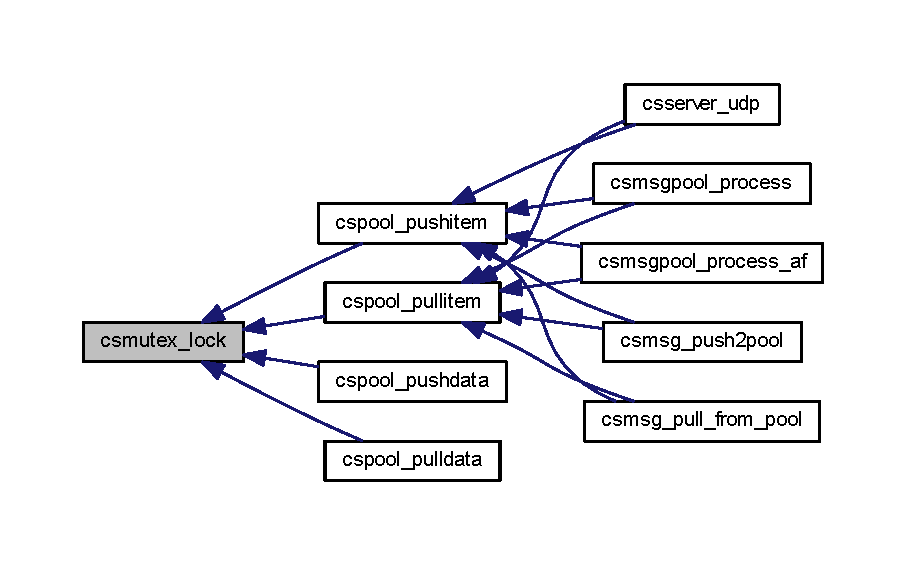
\includegraphics[width=350pt]{lightthread_8c_a78561b071805b213f88d0757b381aa92_icgraph}
\end{center}
\end{figure}


\hypertarget{lightthread_8c_ad3a757691d8d36a947984c914a2fe5b3}{}\index{lightthread.\+c@{lightthread.\+c}!csmutex\+\_\+try\+\_\+lock@{csmutex\+\_\+try\+\_\+lock}}
\index{csmutex\+\_\+try\+\_\+lock@{csmutex\+\_\+try\+\_\+lock}!lightthread.\+c@{lightthread.\+c}}
\subsubsection[{csmutex\+\_\+try\+\_\+lock(csmutex\+\_\+t handle, unsigned int msec)}]{\setlength{\rightskip}{0pt plus 5cm}int csmutex\+\_\+try\+\_\+lock (
\begin{DoxyParamCaption}
\item[{csmutex\+\_\+t}]{handle, }
\item[{unsigned int}]{msec}
\end{DoxyParamCaption}
)}\label{lightthread_8c_ad3a757691d8d36a947984c914a2fe5b3}


csmutex\+\_\+try\+\_\+lock This function returns zero if a lock on the mutex object referenced by mutex is acquired. Otherwise, an error number is returned to indicate the error. 


\begin{DoxyParams}{Parameters}
{\em handle} & handle specify the mutex. \\
\hline
{\em msec} & msec specify the time span to try to lock the mutex.\\
\hline
\end{DoxyParams}
\begin{DoxyReturn}{Returns}

\begin{DoxyEnumerate}
\item 0, if success.
\item -\/1, if timeout.
\item others error code. 
\end{DoxyEnumerate}
\end{DoxyReturn}
\hypertarget{lightthread_8c_abe0d10d1918d0b3fc8a9966e9710b632}{}\index{lightthread.\+c@{lightthread.\+c}!csmutex\+\_\+unlock@{csmutex\+\_\+unlock}}
\index{csmutex\+\_\+unlock@{csmutex\+\_\+unlock}!lightthread.\+c@{lightthread.\+c}}
\subsubsection[{csmutex\+\_\+unlock(csmutex\+\_\+t handle)}]{\setlength{\rightskip}{0pt plus 5cm}void csmutex\+\_\+unlock (
\begin{DoxyParamCaption}
\item[{csmutex\+\_\+t}]{handle}
\end{DoxyParamCaption}
)}\label{lightthread_8c_abe0d10d1918d0b3fc8a9966e9710b632}


csmutex\+\_\+unlock This function unlock the numtex. 


\begin{DoxyParams}{Parameters}
{\em handle} & handle specify the mutex. \\
\hline
\end{DoxyParams}


Here is the caller graph for this function\+:
\nopagebreak
\begin{figure}[H]
\begin{center}
\leavevmode
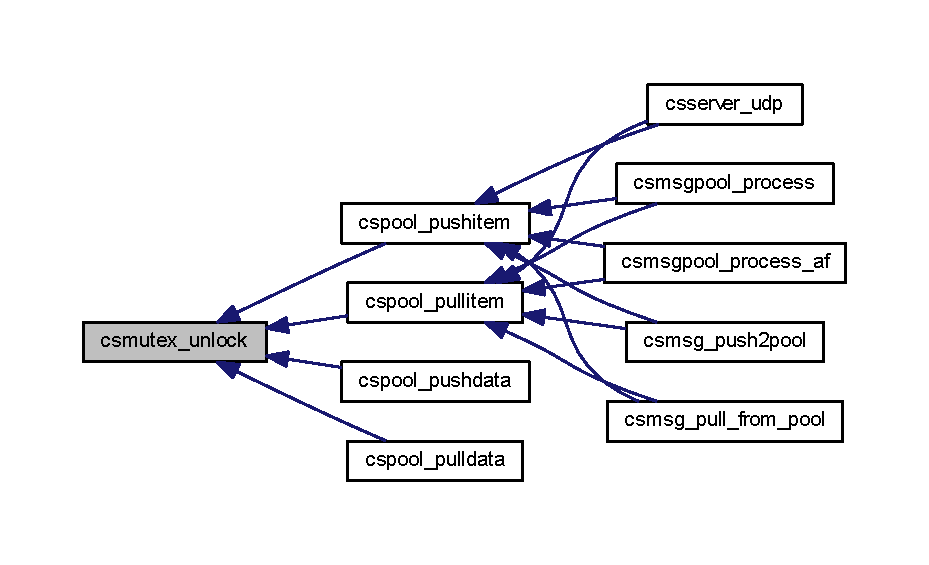
\includegraphics[width=350pt]{lightthread_8c_abe0d10d1918d0b3fc8a9966e9710b632_icgraph}
\end{center}
\end{figure}


\hypertarget{lightthread_8c_a903de2b932fc9de89fd5952d217ddd15}{}\index{lightthread.\+c@{lightthread.\+c}!cssleep@{cssleep}}
\index{cssleep@{cssleep}!lightthread.\+c@{lightthread.\+c}}
\subsubsection[{cssleep(unsigned int msec)}]{\setlength{\rightskip}{0pt plus 5cm}void cssleep (
\begin{DoxyParamCaption}
\item[{unsigned int}]{msec}
\end{DoxyParamCaption}
)}\label{lightthread_8c_a903de2b932fc9de89fd5952d217ddd15}


cssleep 


\begin{DoxyParams}{Parameters}
{\em msec} & \\
\hline
\end{DoxyParams}


Here is the caller graph for this function\+:
\nopagebreak
\begin{figure}[H]
\begin{center}
\leavevmode
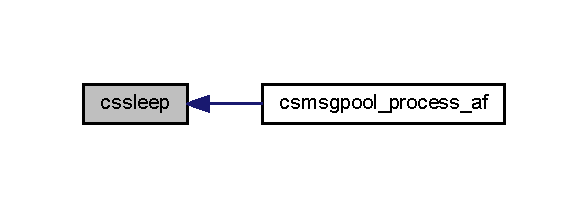
\includegraphics[width=282pt]{lightthread_8c_a903de2b932fc9de89fd5952d217ddd15_icgraph}
\end{center}
\end{figure}


\hypertarget{lightthread_8c_a56ae5a13616435e42ec013020a35cf59}{}\index{lightthread.\+c@{lightthread.\+c}!csthread\+\_\+create@{csthread\+\_\+create}}
\index{csthread\+\_\+create@{csthread\+\_\+create}!lightthread.\+c@{lightthread.\+c}}
\subsubsection[{csthread\+\_\+create(csthread\+\_\+proc\+\_\+t proc, void $\ast$pargs, csthread\+\_\+t $\ast$handle)}]{\setlength{\rightskip}{0pt plus 5cm}int csthread\+\_\+create (
\begin{DoxyParamCaption}
\item[{csthread\+\_\+proc\+\_\+t}]{proc, }
\item[{void $\ast$}]{pargs, }
\item[{csthread\+\_\+t $\ast$}]{handle}
\end{DoxyParamCaption}
)}\label{lightthread_8c_a56ae5a13616435e42ec013020a35cf59}


The following block describe the windows thread functions. 

csthread\+\_\+create

The following block describe the unix thread functions. \hypertarget{lightthread_8c_a16e901a07d7391faed2f6e41af336708}{}\index{lightthread.\+c@{lightthread.\+c}!csthread\+\_\+getpid@{csthread\+\_\+getpid}}
\index{csthread\+\_\+getpid@{csthread\+\_\+getpid}!lightthread.\+c@{lightthread.\+c}}
\subsubsection[{csthread\+\_\+getpid(void)}]{\setlength{\rightskip}{0pt plus 5cm}unsigned int csthread\+\_\+getpid (
\begin{DoxyParamCaption}
\item[{void}]{}
\end{DoxyParamCaption}
)}\label{lightthread_8c_a16e901a07d7391faed2f6e41af336708}


csthread\+\_\+getpid 

\begin{DoxyReturn}{Returns}

\end{DoxyReturn}


Here is the caller graph for this function\+:
\nopagebreak
\begin{figure}[H]
\begin{center}
\leavevmode
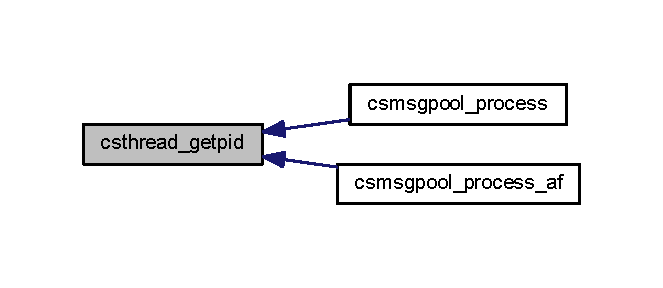
\includegraphics[width=318pt]{lightthread_8c_a16e901a07d7391faed2f6e41af336708_icgraph}
\end{center}
\end{figure}


\hypertarget{lightthread_8c_a3be8a03a3c7ab0758d4dfe1c1a4939dd}{}\index{lightthread.\+c@{lightthread.\+c}!csthread\+\_\+wait\+\_\+terminate@{csthread\+\_\+wait\+\_\+terminate}}
\index{csthread\+\_\+wait\+\_\+terminate@{csthread\+\_\+wait\+\_\+terminate}!lightthread.\+c@{lightthread.\+c}}
\subsubsection[{csthread\+\_\+wait\+\_\+terminate(csthread\+\_\+t handle)}]{\setlength{\rightskip}{0pt plus 5cm}void csthread\+\_\+wait\+\_\+terminate (
\begin{DoxyParamCaption}
\item[{csthread\+\_\+t}]{handle}
\end{DoxyParamCaption}
)}\label{lightthread_8c_a3be8a03a3c7ab0758d4dfe1c1a4939dd}


csthread\+\_\+wait\+\_\+terminate 


\begin{DoxyParams}{Parameters}
{\em handle} & \\
\hline
\end{DoxyParams}


Here is the caller graph for this function\+:
\nopagebreak
\begin{figure}[H]
\begin{center}
\leavevmode
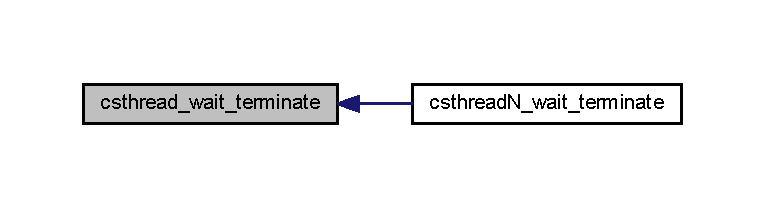
\includegraphics[width=350pt]{lightthread_8c_a3be8a03a3c7ab0758d4dfe1c1a4939dd_icgraph}
\end{center}
\end{figure}


\hypertarget{lightthread_8c_a40598371a661aa6085b63b001f161a71}{}\index{lightthread.\+c@{lightthread.\+c}!csthread\+N\+\_\+wait\+\_\+terminate@{csthread\+N\+\_\+wait\+\_\+terminate}}
\index{csthread\+N\+\_\+wait\+\_\+terminate@{csthread\+N\+\_\+wait\+\_\+terminate}!lightthread.\+c@{lightthread.\+c}}
\subsubsection[{csthread\+N\+\_\+wait\+\_\+terminate(csthread\+\_\+t $\ast$handle, int count)}]{\setlength{\rightskip}{0pt plus 5cm}void csthread\+N\+\_\+wait\+\_\+terminate (
\begin{DoxyParamCaption}
\item[{csthread\+\_\+t $\ast$}]{handle, }
\item[{int}]{count}
\end{DoxyParamCaption}
)}\label{lightthread_8c_a40598371a661aa6085b63b001f161a71}


csthread\+N\+\_\+wait\+\_\+terminate 


\begin{DoxyParams}{Parameters}
{\em handle} & \\
\hline
{\em count} & \\
\hline
\end{DoxyParams}


Here is the call graph for this function\+:
\nopagebreak
\begin{figure}[H]
\begin{center}
\leavevmode
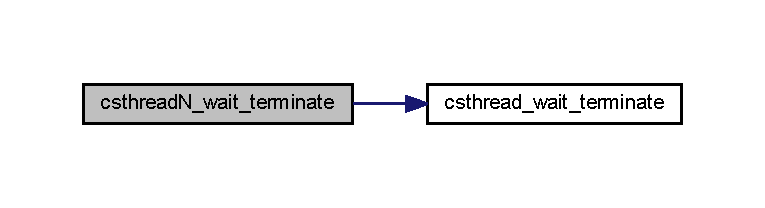
\includegraphics[width=350pt]{lightthread_8c_a40598371a661aa6085b63b001f161a71_cgraph}
\end{center}
\end{figure}



\hypertarget{lightthread_8h}{}\section{D\+:/project/\+Peng\+Ge/client\+\_\+server/src/common/lightthread.h File Reference}
\label{lightthread_8h}\index{D\+:/project/\+Peng\+Ge/client\+\_\+server/src/common/lightthread.\+h@{D\+:/project/\+Peng\+Ge/client\+\_\+server/src/common/lightthread.\+h}}


This file defines some basic wrapper functions of thread, mutex and semaphore.  


This graph shows which files directly or indirectly include this file\+:
\nopagebreak
\begin{figure}[H]
\begin{center}
\leavevmode
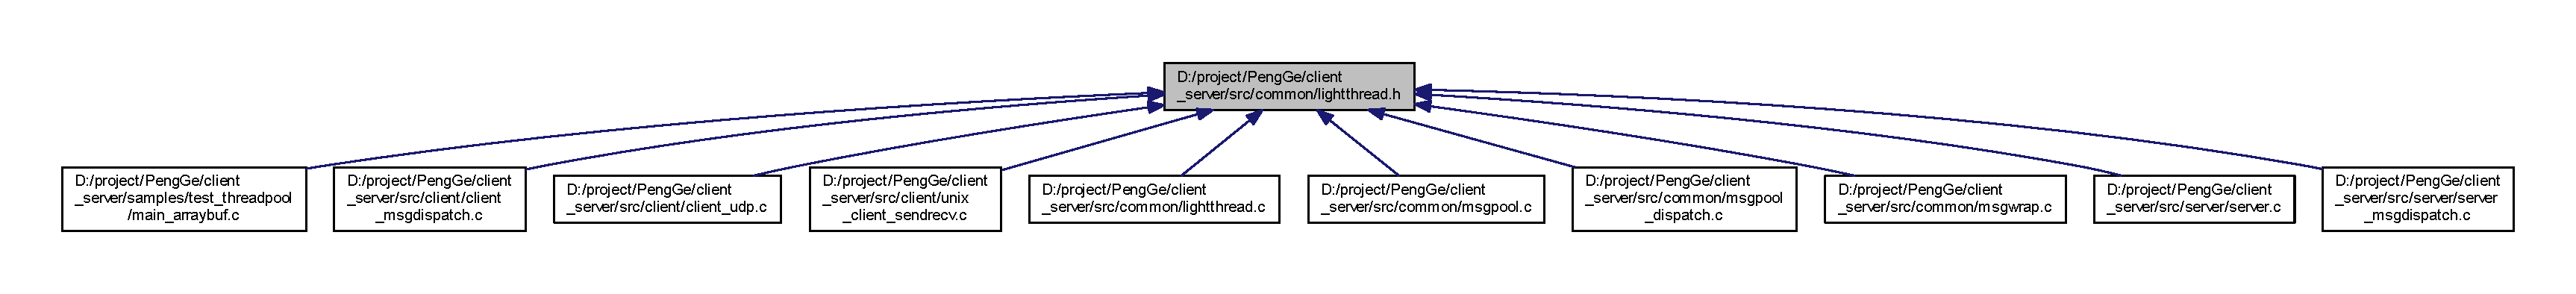
\includegraphics[width=350pt]{lightthread_8h__dep__incl}
\end{center}
\end{figure}
\subsection*{Macros}
\begin{DoxyCompactItemize}
\item 
\hypertarget{lightthread_8h_aa3b671eedc1c42b33634b91da858fb71}{}\#define {\bfseries cssem\+\_\+wait}~sem\+\_\+wait\label{lightthread_8h_aa3b671eedc1c42b33634b91da858fb71}

\item 
\hypertarget{lightthread_8h_a2dea9ea8cb965c134a53c5260817afc1}{}\#define {\bfseries cssem\+\_\+post}~sem\+\_\+post\label{lightthread_8h_a2dea9ea8cb965c134a53c5260817afc1}

\item 
\hypertarget{lightthread_8h_aa7d66b30f3d06b2f211bd016dcaf23f4}{}\#define {\bfseries cssem\+\_\+destroy}~sem\+\_\+destroy\label{lightthread_8h_aa7d66b30f3d06b2f211bd016dcaf23f4}

\end{DoxyCompactItemize}
\subsection*{Typedefs}
\begin{DoxyCompactItemize}
\item 
\hypertarget{lightthread_8h_abb7c984a936823027eddd6bdf6584e9b}{}typedef pthread\+\_\+mutex\+\_\+t {\bfseries csmutex\+\_\+t}\label{lightthread_8h_abb7c984a936823027eddd6bdf6584e9b}

\item 
\hypertarget{lightthread_8h_a57986cb36f70ef3cb073481f6dfbf367}{}typedef sem\+\_\+t {\bfseries cssem\+\_\+t}\label{lightthread_8h_a57986cb36f70ef3cb073481f6dfbf367}

\item 
\hypertarget{lightthread_8h_a40498c08ce5d1d40ae8095e4d373c080}{}typedef pthread\+\_\+t {\bfseries csthread\+\_\+t}\label{lightthread_8h_a40498c08ce5d1d40ae8095e4d373c080}

\item 
\hypertarget{lightthread_8h_a11acaad034da6c34f500602ff914ffff}{}typedef void $\ast$($\ast$ {\bfseries csthread\+\_\+proc\+\_\+t}) (void $\ast$)\label{lightthread_8h_a11acaad034da6c34f500602ff914ffff}

\end{DoxyCompactItemize}
\subsection*{Functions}
\begin{DoxyCompactItemize}
\item 
int \hyperlink{lightthread_8h_a56ae5a13616435e42ec013020a35cf59}{csthread\+\_\+create} (csthread\+\_\+proc\+\_\+t proc, void $\ast$pargs, csthread\+\_\+t $\ast$handle)
\begin{DoxyCompactList}\small\item\em csthread\+\_\+create \end{DoxyCompactList}\item 
\hypertarget{lightthread_8h_a3f281b2855e0eb63360f12a1e745e088}{}void \hyperlink{lightthread_8h_a3f281b2855e0eb63360f12a1e745e088}{csthread\+\_\+exit} (void)\label{lightthread_8h_a3f281b2855e0eb63360f12a1e745e088}

\begin{DoxyCompactList}\small\item\em csthread\+\_\+exit \end{DoxyCompactList}\item 
void \hyperlink{lightthread_8h_a3be8a03a3c7ab0758d4dfe1c1a4939dd}{csthread\+\_\+wait\+\_\+terminate} (csthread\+\_\+t handle)
\begin{DoxyCompactList}\small\item\em csthread\+\_\+wait\+\_\+terminate \end{DoxyCompactList}\item 
void \hyperlink{lightthread_8h_a40598371a661aa6085b63b001f161a71}{csthread\+N\+\_\+wait\+\_\+terminate} (csthread\+\_\+t $\ast$handle, int count)
\begin{DoxyCompactList}\small\item\em csthread\+N\+\_\+wait\+\_\+terminate \end{DoxyCompactList}\item 
unsigned int \hyperlink{lightthread_8h_a16e901a07d7391faed2f6e41af336708}{csthread\+\_\+getpid} (void)
\begin{DoxyCompactList}\small\item\em csthread\+\_\+getpid \end{DoxyCompactList}\item 
void \hyperlink{lightthread_8h_a903de2b932fc9de89fd5952d217ddd15}{cssleep} (unsigned int msec)
\begin{DoxyCompactList}\small\item\em cssleep \end{DoxyCompactList}\item 
csmutex\+\_\+t \hyperlink{lightthread_8h_a5c3a7fb06b62b05a6dfa3359eb939655}{csmutex\+\_\+create} (void)
\begin{DoxyCompactList}\small\item\em csmutex\+\_\+create csmutex\+\_\+create will create the mutex and print error message if error occurs. \end{DoxyCompactList}\item 
void \hyperlink{lightthread_8h_aab46494a34bf1e3dbd157b8dd6ea04cb}{csmutex\+\_\+destroy} (csmutex\+\_\+t handle)
\begin{DoxyCompactList}\small\item\em csmutex\+\_\+destroy \end{DoxyCompactList}\item 
int \hyperlink{lightthread_8h_a78561b071805b213f88d0757b381aa92}{csmutex\+\_\+lock} (csmutex\+\_\+t handle)
\begin{DoxyCompactList}\small\item\em csmutex\+\_\+lock \end{DoxyCompactList}\item 
int \hyperlink{lightthread_8h_ad3a757691d8d36a947984c914a2fe5b3}{csmutex\+\_\+try\+\_\+lock} (csmutex\+\_\+t handle, unsigned int msec)
\begin{DoxyCompactList}\small\item\em csmutex\+\_\+try\+\_\+lock This function returns zero if a lock on the mutex object referenced by mutex is acquired. Otherwise, an error number is returned to indicate the error. \end{DoxyCompactList}\item 
void \hyperlink{lightthread_8h_abe0d10d1918d0b3fc8a9966e9710b632}{csmutex\+\_\+unlock} (csmutex\+\_\+t handle)
\begin{DoxyCompactList}\small\item\em csmutex\+\_\+unlock This function unlock the numtex. \end{DoxyCompactList}\item 
\hypertarget{lightthread_8h_a28c2302dea7cc0ccaa65453cc5dabead}{}int {\bfseries cssem\+\_\+create} (int value\+\_\+init, int value\+\_\+max, cssem\+\_\+t $\ast$handle)\label{lightthread_8h_a28c2302dea7cc0ccaa65453cc5dabead}

\end{DoxyCompactItemize}


\subsection{Detailed Description}
This file defines some basic wrapper functions of thread, mutex and semaphore. 

\begin{DoxyAuthor}{Author}
cxl, \href{mailto:shuanglongchen@yeah.net}{\tt shuanglongchen@yeah.\+net} 
\end{DoxyAuthor}
\begin{DoxyVersion}{Version}
0.\+1 
\end{DoxyVersion}
\begin{DoxyDate}{Date}
2015-\/10-\/26 
\end{DoxyDate}
\begin{DoxyParagraph}{last modified}
2015-\/10-\/28 00\+:56\+:06 (+0800) 
\end{DoxyParagraph}


\subsection{Function Documentation}
\hypertarget{lightthread_8h_a5c3a7fb06b62b05a6dfa3359eb939655}{}\index{lightthread.\+h@{lightthread.\+h}!csmutex\+\_\+create@{csmutex\+\_\+create}}
\index{csmutex\+\_\+create@{csmutex\+\_\+create}!lightthread.\+h@{lightthread.\+h}}
\subsubsection[{csmutex\+\_\+create(void)}]{\setlength{\rightskip}{0pt plus 5cm}csmutex\+\_\+t csmutex\+\_\+create (
\begin{DoxyParamCaption}
\item[{void}]{}
\end{DoxyParamCaption}
)}\label{lightthread_8h_a5c3a7fb06b62b05a6dfa3359eb939655}


csmutex\+\_\+create csmutex\+\_\+create will create the mutex and print error message if error occurs. 

\begin{DoxyReturn}{Returns}
N\+U\+L\+L if failed; valid mutex handle if succes. 
\end{DoxyReturn}
\hypertarget{lightthread_8h_aab46494a34bf1e3dbd157b8dd6ea04cb}{}\index{lightthread.\+h@{lightthread.\+h}!csmutex\+\_\+destroy@{csmutex\+\_\+destroy}}
\index{csmutex\+\_\+destroy@{csmutex\+\_\+destroy}!lightthread.\+h@{lightthread.\+h}}
\subsubsection[{csmutex\+\_\+destroy(csmutex\+\_\+t handle)}]{\setlength{\rightskip}{0pt plus 5cm}void csmutex\+\_\+destroy (
\begin{DoxyParamCaption}
\item[{csmutex\+\_\+t}]{handle}
\end{DoxyParamCaption}
)}\label{lightthread_8h_aab46494a34bf1e3dbd157b8dd6ea04cb}


csmutex\+\_\+destroy 


\begin{DoxyParams}{Parameters}
{\em handle} & \\
\hline
\end{DoxyParams}
\hypertarget{lightthread_8h_a78561b071805b213f88d0757b381aa92}{}\index{lightthread.\+h@{lightthread.\+h}!csmutex\+\_\+lock@{csmutex\+\_\+lock}}
\index{csmutex\+\_\+lock@{csmutex\+\_\+lock}!lightthread.\+h@{lightthread.\+h}}
\subsubsection[{csmutex\+\_\+lock(csmutex\+\_\+t handle)}]{\setlength{\rightskip}{0pt plus 5cm}int csmutex\+\_\+lock (
\begin{DoxyParamCaption}
\item[{csmutex\+\_\+t}]{handle}
\end{DoxyParamCaption}
)}\label{lightthread_8h_a78561b071805b213f88d0757b381aa92}


csmutex\+\_\+lock 


\begin{DoxyParams}{Parameters}
{\em handle} & \\
\hline
\end{DoxyParams}
\begin{DoxyReturn}{Returns}
0 if O\+K; -\/1 if failed. 
\end{DoxyReturn}


Here is the caller graph for this function\+:
\nopagebreak
\begin{figure}[H]
\begin{center}
\leavevmode
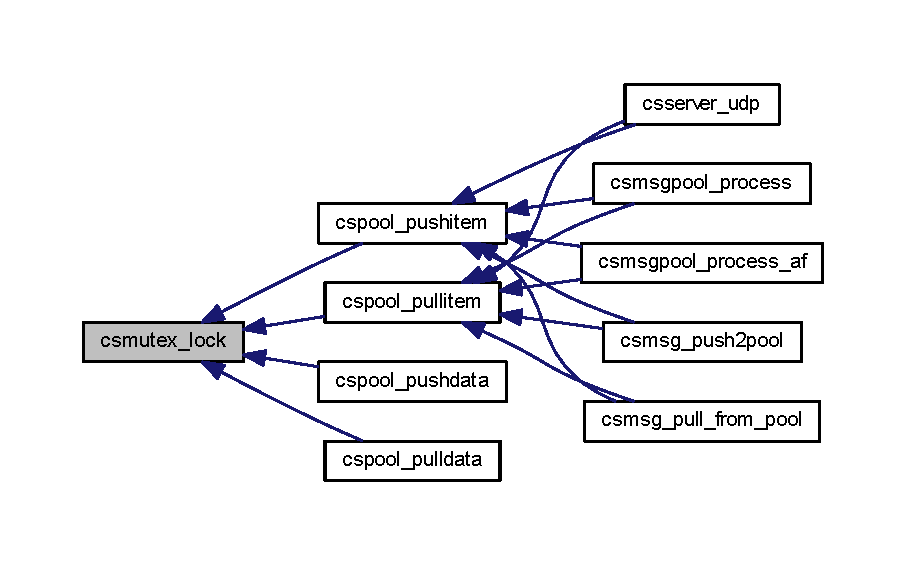
\includegraphics[width=350pt]{lightthread_8h_a78561b071805b213f88d0757b381aa92_icgraph}
\end{center}
\end{figure}


\hypertarget{lightthread_8h_ad3a757691d8d36a947984c914a2fe5b3}{}\index{lightthread.\+h@{lightthread.\+h}!csmutex\+\_\+try\+\_\+lock@{csmutex\+\_\+try\+\_\+lock}}
\index{csmutex\+\_\+try\+\_\+lock@{csmutex\+\_\+try\+\_\+lock}!lightthread.\+h@{lightthread.\+h}}
\subsubsection[{csmutex\+\_\+try\+\_\+lock(csmutex\+\_\+t handle, unsigned int msec)}]{\setlength{\rightskip}{0pt plus 5cm}int csmutex\+\_\+try\+\_\+lock (
\begin{DoxyParamCaption}
\item[{csmutex\+\_\+t}]{handle, }
\item[{unsigned int}]{msec}
\end{DoxyParamCaption}
)}\label{lightthread_8h_ad3a757691d8d36a947984c914a2fe5b3}


csmutex\+\_\+try\+\_\+lock This function returns zero if a lock on the mutex object referenced by mutex is acquired. Otherwise, an error number is returned to indicate the error. 


\begin{DoxyParams}{Parameters}
{\em handle} & handle specify the mutex. \\
\hline
{\em msec} & msec specify the time span to try to lock the mutex.\\
\hline
\end{DoxyParams}
\begin{DoxyReturn}{Returns}

\begin{DoxyEnumerate}
\item 0, if success.
\item -\/1, if timeout.
\item others error code. 
\end{DoxyEnumerate}
\end{DoxyReturn}
\hypertarget{lightthread_8h_abe0d10d1918d0b3fc8a9966e9710b632}{}\index{lightthread.\+h@{lightthread.\+h}!csmutex\+\_\+unlock@{csmutex\+\_\+unlock}}
\index{csmutex\+\_\+unlock@{csmutex\+\_\+unlock}!lightthread.\+h@{lightthread.\+h}}
\subsubsection[{csmutex\+\_\+unlock(csmutex\+\_\+t handle)}]{\setlength{\rightskip}{0pt plus 5cm}void csmutex\+\_\+unlock (
\begin{DoxyParamCaption}
\item[{csmutex\+\_\+t}]{handle}
\end{DoxyParamCaption}
)}\label{lightthread_8h_abe0d10d1918d0b3fc8a9966e9710b632}


csmutex\+\_\+unlock This function unlock the numtex. 


\begin{DoxyParams}{Parameters}
{\em handle} & handle specify the mutex. \\
\hline
\end{DoxyParams}


Here is the caller graph for this function\+:
\nopagebreak
\begin{figure}[H]
\begin{center}
\leavevmode
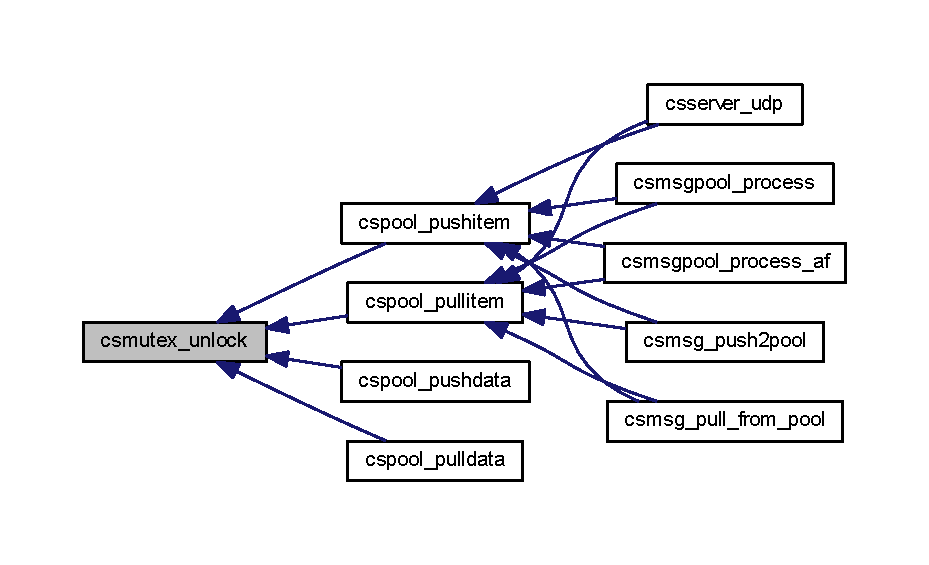
\includegraphics[width=350pt]{lightthread_8h_abe0d10d1918d0b3fc8a9966e9710b632_icgraph}
\end{center}
\end{figure}


\hypertarget{lightthread_8h_a903de2b932fc9de89fd5952d217ddd15}{}\index{lightthread.\+h@{lightthread.\+h}!cssleep@{cssleep}}
\index{cssleep@{cssleep}!lightthread.\+h@{lightthread.\+h}}
\subsubsection[{cssleep(unsigned int msec)}]{\setlength{\rightskip}{0pt plus 5cm}void cssleep (
\begin{DoxyParamCaption}
\item[{unsigned int}]{msec}
\end{DoxyParamCaption}
)}\label{lightthread_8h_a903de2b932fc9de89fd5952d217ddd15}


cssleep 


\begin{DoxyParams}{Parameters}
{\em msec} & \\
\hline
\end{DoxyParams}


Here is the caller graph for this function\+:
\nopagebreak
\begin{figure}[H]
\begin{center}
\leavevmode
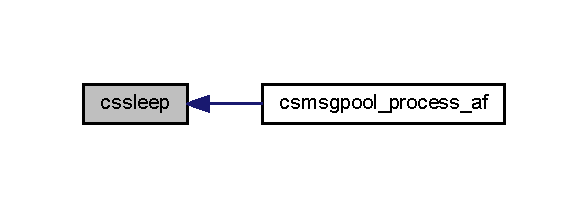
\includegraphics[width=282pt]{lightthread_8h_a903de2b932fc9de89fd5952d217ddd15_icgraph}
\end{center}
\end{figure}


\hypertarget{lightthread_8h_a56ae5a13616435e42ec013020a35cf59}{}\index{lightthread.\+h@{lightthread.\+h}!csthread\+\_\+create@{csthread\+\_\+create}}
\index{csthread\+\_\+create@{csthread\+\_\+create}!lightthread.\+h@{lightthread.\+h}}
\subsubsection[{csthread\+\_\+create(csthread\+\_\+proc\+\_\+t proc, void $\ast$pargs, csthread\+\_\+t $\ast$handle)}]{\setlength{\rightskip}{0pt plus 5cm}int csthread\+\_\+create (
\begin{DoxyParamCaption}
\item[{csthread\+\_\+proc\+\_\+t}]{proc, }
\item[{void $\ast$}]{pargs, }
\item[{csthread\+\_\+t $\ast$}]{handle}
\end{DoxyParamCaption}
)}\label{lightthread_8h_a56ae5a13616435e42ec013020a35cf59}


csthread\+\_\+create 


\begin{DoxyParams}{Parameters}
{\em proc} & \\
\hline
{\em pargs} & the thread handle\\
\hline
\end{DoxyParams}
\begin{DoxyReturn}{Returns}

\end{DoxyReturn}
csthread\+\_\+create

The following block describe the unix thread functions. \hypertarget{lightthread_8h_a16e901a07d7391faed2f6e41af336708}{}\index{lightthread.\+h@{lightthread.\+h}!csthread\+\_\+getpid@{csthread\+\_\+getpid}}
\index{csthread\+\_\+getpid@{csthread\+\_\+getpid}!lightthread.\+h@{lightthread.\+h}}
\subsubsection[{csthread\+\_\+getpid(void)}]{\setlength{\rightskip}{0pt plus 5cm}unsigned int csthread\+\_\+getpid (
\begin{DoxyParamCaption}
\item[{void}]{}
\end{DoxyParamCaption}
)}\label{lightthread_8h_a16e901a07d7391faed2f6e41af336708}


csthread\+\_\+getpid 

\begin{DoxyReturn}{Returns}

\end{DoxyReturn}


Here is the caller graph for this function\+:
\nopagebreak
\begin{figure}[H]
\begin{center}
\leavevmode
\includegraphics[width=318pt]{lightthread_8h_a16e901a07d7391faed2f6e41af336708_icgraph}
\end{center}
\end{figure}


\hypertarget{lightthread_8h_a3be8a03a3c7ab0758d4dfe1c1a4939dd}{}\index{lightthread.\+h@{lightthread.\+h}!csthread\+\_\+wait\+\_\+terminate@{csthread\+\_\+wait\+\_\+terminate}}
\index{csthread\+\_\+wait\+\_\+terminate@{csthread\+\_\+wait\+\_\+terminate}!lightthread.\+h@{lightthread.\+h}}
\subsubsection[{csthread\+\_\+wait\+\_\+terminate(csthread\+\_\+t handle)}]{\setlength{\rightskip}{0pt plus 5cm}void csthread\+\_\+wait\+\_\+terminate (
\begin{DoxyParamCaption}
\item[{csthread\+\_\+t}]{handle}
\end{DoxyParamCaption}
)}\label{lightthread_8h_a3be8a03a3c7ab0758d4dfe1c1a4939dd}


csthread\+\_\+wait\+\_\+terminate 


\begin{DoxyParams}{Parameters}
{\em handle} & \\
\hline
\end{DoxyParams}


Here is the caller graph for this function\+:
\nopagebreak
\begin{figure}[H]
\begin{center}
\leavevmode
\includegraphics[width=350pt]{lightthread_8h_a3be8a03a3c7ab0758d4dfe1c1a4939dd_icgraph}
\end{center}
\end{figure}


\hypertarget{lightthread_8h_a40598371a661aa6085b63b001f161a71}{}\index{lightthread.\+h@{lightthread.\+h}!csthread\+N\+\_\+wait\+\_\+terminate@{csthread\+N\+\_\+wait\+\_\+terminate}}
\index{csthread\+N\+\_\+wait\+\_\+terminate@{csthread\+N\+\_\+wait\+\_\+terminate}!lightthread.\+h@{lightthread.\+h}}
\subsubsection[{csthread\+N\+\_\+wait\+\_\+terminate(csthread\+\_\+t $\ast$handle, int count)}]{\setlength{\rightskip}{0pt plus 5cm}void csthread\+N\+\_\+wait\+\_\+terminate (
\begin{DoxyParamCaption}
\item[{csthread\+\_\+t $\ast$}]{handle, }
\item[{int}]{count}
\end{DoxyParamCaption}
)}\label{lightthread_8h_a40598371a661aa6085b63b001f161a71}


csthread\+N\+\_\+wait\+\_\+terminate 


\begin{DoxyParams}{Parameters}
{\em handle} & \\
\hline
{\em count} & \\
\hline
\end{DoxyParams}


Here is the call graph for this function\+:
\nopagebreak
\begin{figure}[H]
\begin{center}
\leavevmode
\includegraphics[width=350pt]{lightthread_8h_a40598371a661aa6085b63b001f161a71_cgraph}
\end{center}
\end{figure}



\hypertarget{list_8c}{}\section{D\+:/project/\+Peng\+Ge/client\+\_\+server/src/common/list.c File Reference}
\label{list_8c}\index{D\+:/project/\+Peng\+Ge/client\+\_\+server/src/common/list.\+c@{D\+:/project/\+Peng\+Ge/client\+\_\+server/src/common/list.\+c}}
{\ttfamily \#include \char`\"{}list.\+h\char`\"{}}\\*
Include dependency graph for list.\+c\+:
\nopagebreak
\begin{figure}[H]
\begin{center}
\leavevmode
\includegraphics[width=208pt]{list_8c__incl}
\end{center}
\end{figure}
\subsection*{Functions}
\begin{DoxyCompactItemize}
\item 
\hypertarget{list_8c_af8fefe2d35c3f2ef3a3fc693d0080c48}{}void {\bfseries I\+N\+I\+T\+\_\+\+L\+I\+S\+T\+\_\+\+H\+E\+A\+D} (struct \hyperlink{structlist__head}{list\+\_\+head} $\ast$list)\label{list_8c_af8fefe2d35c3f2ef3a3fc693d0080c48}

\item 
void \hyperlink{list_8c_a221a74d55162a5f9351c3ad989fa08f4}{list\+\_\+add} (struct \hyperlink{structlist__head}{list\+\_\+head} $\ast$new, struct \hyperlink{structlist__head}{list\+\_\+head} $\ast$head)
\item 
void \hyperlink{list_8c_a7de7ab829b695186fc3d07e408b1efa6}{list\+\_\+add\+\_\+tail} (struct \hyperlink{structlist__head}{list\+\_\+head} $\ast$new, struct \hyperlink{structlist__head}{list\+\_\+head} $\ast$head)
\item 
void \hyperlink{list_8c_ac32a18fe87fa883f9679ca4bc4b88693}{list\+\_\+del} (struct \hyperlink{structlist__head}{list\+\_\+head} $\ast$entry)
\item 
void \hyperlink{list_8c_a8c973321bd3e45debe536e5241e1ac0d}{list\+\_\+replace} (struct \hyperlink{structlist__head}{list\+\_\+head} $\ast$old, struct \hyperlink{structlist__head}{list\+\_\+head} $\ast$new)
\item 
int \hyperlink{list_8c_ac2f0fecd0fceee7e5a9cb5550639e87a}{list\+\_\+is\+\_\+last} (const struct \hyperlink{structlist__head}{list\+\_\+head} $\ast$list, const struct \hyperlink{structlist__head}{list\+\_\+head} $\ast$head)
\item 
int \hyperlink{list_8c_ac3f49962b8b320c32f3b28ec0f94bd36}{list\+\_\+empty} (const struct \hyperlink{structlist__head}{list\+\_\+head} $\ast$head)
\end{DoxyCompactItemize}


\subsection{Detailed Description}
\begin{DoxyAuthor}{Author}
cxl, \href{mailto:shuanglongchen@yeah.net}{\tt shuanglongchen@yeah.\+net} 
\end{DoxyAuthor}
\begin{DoxyVersion}{Version}
0.\+1 
\end{DoxyVersion}
\begin{DoxyDate}{Date}
2015-\/10-\/16 
\end{DoxyDate}


\subsection{Function Documentation}
\hypertarget{list_8c_a221a74d55162a5f9351c3ad989fa08f4}{}\index{list.\+c@{list.\+c}!list\+\_\+add@{list\+\_\+add}}
\index{list\+\_\+add@{list\+\_\+add}!list.\+c@{list.\+c}}
\subsubsection[{list\+\_\+add(struct list\+\_\+head $\ast$new, struct list\+\_\+head $\ast$head)}]{\setlength{\rightskip}{0pt plus 5cm}void list\+\_\+add (
\begin{DoxyParamCaption}
\item[{struct {\bf list\+\_\+head} $\ast$}]{new, }
\item[{struct {\bf list\+\_\+head} $\ast$}]{head}
\end{DoxyParamCaption}
)}\label{list_8c_a221a74d55162a5f9351c3ad989fa08f4}
list\+\_\+add -\/ add a new entry \+: new entry to be added \+: list head to add it after

Insert a new entry after the specified head. This is good for implementing stacks. \hypertarget{list_8c_a7de7ab829b695186fc3d07e408b1efa6}{}\index{list.\+c@{list.\+c}!list\+\_\+add\+\_\+tail@{list\+\_\+add\+\_\+tail}}
\index{list\+\_\+add\+\_\+tail@{list\+\_\+add\+\_\+tail}!list.\+c@{list.\+c}}
\subsubsection[{list\+\_\+add\+\_\+tail(struct list\+\_\+head $\ast$new, struct list\+\_\+head $\ast$head)}]{\setlength{\rightskip}{0pt plus 5cm}void list\+\_\+add\+\_\+tail (
\begin{DoxyParamCaption}
\item[{struct {\bf list\+\_\+head} $\ast$}]{new, }
\item[{struct {\bf list\+\_\+head} $\ast$}]{head}
\end{DoxyParamCaption}
)}\label{list_8c_a7de7ab829b695186fc3d07e408b1efa6}
list\+\_\+add\+\_\+tail -\/ add a new entry \+: new entry to be added \+: list head to add it before

Insert a new entry before the specified head. This is useful for implementing queues. \hypertarget{list_8c_ac32a18fe87fa883f9679ca4bc4b88693}{}\index{list.\+c@{list.\+c}!list\+\_\+del@{list\+\_\+del}}
\index{list\+\_\+del@{list\+\_\+del}!list.\+c@{list.\+c}}
\subsubsection[{list\+\_\+del(struct list\+\_\+head $\ast$entry)}]{\setlength{\rightskip}{0pt plus 5cm}void list\+\_\+del (
\begin{DoxyParamCaption}
\item[{struct {\bf list\+\_\+head} $\ast$}]{entry}
\end{DoxyParamCaption}
)}\label{list_8c_ac32a18fe87fa883f9679ca4bc4b88693}
list\+\_\+del -\/ deletes entry from list. \+: the element to delete from the list. Note\+: \hyperlink{list_8c_ac3f49962b8b320c32f3b28ec0f94bd36}{list\+\_\+empty()} on entry does not return true after this, the entry is in an undefined state. \hypertarget{list_8c_ac3f49962b8b320c32f3b28ec0f94bd36}{}\index{list.\+c@{list.\+c}!list\+\_\+empty@{list\+\_\+empty}}
\index{list\+\_\+empty@{list\+\_\+empty}!list.\+c@{list.\+c}}
\subsubsection[{list\+\_\+empty(const struct list\+\_\+head $\ast$head)}]{\setlength{\rightskip}{0pt plus 5cm}int list\+\_\+empty (
\begin{DoxyParamCaption}
\item[{const struct {\bf list\+\_\+head} $\ast$}]{head}
\end{DoxyParamCaption}
)}\label{list_8c_ac3f49962b8b320c32f3b28ec0f94bd36}
list\+\_\+empty -\/ tests whether a list is empty \+: the list to test. \hypertarget{list_8c_ac2f0fecd0fceee7e5a9cb5550639e87a}{}\index{list.\+c@{list.\+c}!list\+\_\+is\+\_\+last@{list\+\_\+is\+\_\+last}}
\index{list\+\_\+is\+\_\+last@{list\+\_\+is\+\_\+last}!list.\+c@{list.\+c}}
\subsubsection[{list\+\_\+is\+\_\+last(const struct list\+\_\+head $\ast$list, const struct list\+\_\+head $\ast$head)}]{\setlength{\rightskip}{0pt plus 5cm}int list\+\_\+is\+\_\+last (
\begin{DoxyParamCaption}
\item[{const struct {\bf list\+\_\+head} $\ast$}]{list, }
\item[{const struct {\bf list\+\_\+head} $\ast$}]{head}
\end{DoxyParamCaption}
)}\label{list_8c_ac2f0fecd0fceee7e5a9cb5550639e87a}
list\+\_\+is\+\_\+last -\/ tests whether  is the last entry in list  \+: the entry to test \+: the head of the list \hypertarget{list_8c_a8c973321bd3e45debe536e5241e1ac0d}{}\index{list.\+c@{list.\+c}!list\+\_\+replace@{list\+\_\+replace}}
\index{list\+\_\+replace@{list\+\_\+replace}!list.\+c@{list.\+c}}
\subsubsection[{list\+\_\+replace(struct list\+\_\+head $\ast$old, struct list\+\_\+head $\ast$new)}]{\setlength{\rightskip}{0pt plus 5cm}void list\+\_\+replace (
\begin{DoxyParamCaption}
\item[{struct {\bf list\+\_\+head} $\ast$}]{old, }
\item[{struct {\bf list\+\_\+head} $\ast$}]{new}
\end{DoxyParamCaption}
)}\label{list_8c_a8c973321bd3e45debe536e5241e1ac0d}
list\+\_\+replace -\/ replace old entry by new one  \+: the element to be replaced  \+: the new element to insert

If  was empty, it will be overwritten. 
\hypertarget{list_8h}{}\section{D\+:/project/\+Peng\+Ge/client\+\_\+server/src/common/list.h File Reference}
\label{list_8h}\index{D\+:/project/\+Peng\+Ge/client\+\_\+server/src/common/list.\+h@{D\+:/project/\+Peng\+Ge/client\+\_\+server/src/common/list.\+h}}


This file comes from linux source code. Some unused functions are castrated.  


This graph shows which files directly or indirectly include this file\+:
\nopagebreak
\begin{figure}[H]
\begin{center}
\leavevmode
\includegraphics[width=350pt]{list_8h__dep__incl}
\end{center}
\end{figure}
\subsection*{Classes}
\begin{DoxyCompactItemize}
\item 
struct \hyperlink{structlist__head}{list\+\_\+head}
\end{DoxyCompactItemize}
\subsection*{Macros}
\begin{DoxyCompactItemize}
\item 
\hypertarget{list_8h_a4642d4b7df28478bb762fe43c85b5c63}{}\#define {\bfseries L\+I\+S\+T\+\_\+\+H\+E\+A\+D\+\_\+\+I\+N\+I\+T}(name)~\{ \&(name), \&(name) \}\label{list_8h_a4642d4b7df28478bb762fe43c85b5c63}

\item 
\hypertarget{list_8h_a42f0e72af970a790b60a740af8c9ecd0}{}\#define {\bfseries L\+I\+S\+T\+\_\+\+H\+E\+A\+D}(name)~struct \hyperlink{structlist__head}{list\+\_\+head} name = L\+I\+S\+T\+\_\+\+H\+E\+A\+D\+\_\+\+I\+N\+I\+T(name)\label{list_8h_a42f0e72af970a790b60a740af8c9ecd0}

\end{DoxyCompactItemize}
\subsection*{Functions}
\begin{DoxyCompactItemize}
\item 
\hypertarget{list_8h_af8fefe2d35c3f2ef3a3fc693d0080c48}{}void {\bfseries I\+N\+I\+T\+\_\+\+L\+I\+S\+T\+\_\+\+H\+E\+A\+D} (struct \hyperlink{structlist__head}{list\+\_\+head} $\ast$list)\label{list_8h_af8fefe2d35c3f2ef3a3fc693d0080c48}

\item 
void \hyperlink{list_8h_a221a74d55162a5f9351c3ad989fa08f4}{list\+\_\+add} (struct \hyperlink{structlist__head}{list\+\_\+head} $\ast$new, struct \hyperlink{structlist__head}{list\+\_\+head} $\ast$head)
\item 
void \hyperlink{list_8h_a7de7ab829b695186fc3d07e408b1efa6}{list\+\_\+add\+\_\+tail} (struct \hyperlink{structlist__head}{list\+\_\+head} $\ast$new, struct \hyperlink{structlist__head}{list\+\_\+head} $\ast$head)
\item 
void \hyperlink{list_8h_ac32a18fe87fa883f9679ca4bc4b88693}{list\+\_\+del} (struct \hyperlink{structlist__head}{list\+\_\+head} $\ast$entry)
\item 
void \hyperlink{list_8h_a8c973321bd3e45debe536e5241e1ac0d}{list\+\_\+replace} (struct \hyperlink{structlist__head}{list\+\_\+head} $\ast$old, struct \hyperlink{structlist__head}{list\+\_\+head} $\ast$new)
\item 
int \hyperlink{list_8h_ac2f0fecd0fceee7e5a9cb5550639e87a}{list\+\_\+is\+\_\+last} (const struct \hyperlink{structlist__head}{list\+\_\+head} $\ast$list, const struct \hyperlink{structlist__head}{list\+\_\+head} $\ast$head)
\item 
int \hyperlink{list_8h_ac3f49962b8b320c32f3b28ec0f94bd36}{list\+\_\+empty} (const struct \hyperlink{structlist__head}{list\+\_\+head} $\ast$head)
\end{DoxyCompactItemize}


\subsection{Detailed Description}
This file comes from linux source code. Some unused functions are castrated. 

\begin{DoxyAuthor}{Author}
cxl, \href{mailto:shuanglongchen@yeah.net}{\tt shuanglongchen@yeah.\+net} 
\end{DoxyAuthor}
\begin{DoxyVersion}{Version}
0.\+1 
\end{DoxyVersion}
\begin{DoxyDate}{Date}
2015-\/10-\/16 
\end{DoxyDate}


\subsection{Function Documentation}
\hypertarget{list_8h_a221a74d55162a5f9351c3ad989fa08f4}{}\index{list.\+h@{list.\+h}!list\+\_\+add@{list\+\_\+add}}
\index{list\+\_\+add@{list\+\_\+add}!list.\+h@{list.\+h}}
\subsubsection[{list\+\_\+add(struct list\+\_\+head $\ast$new, struct list\+\_\+head $\ast$head)}]{\setlength{\rightskip}{0pt plus 5cm}void list\+\_\+add (
\begin{DoxyParamCaption}
\item[{struct {\bf list\+\_\+head} $\ast$}]{new, }
\item[{struct {\bf list\+\_\+head} $\ast$}]{head}
\end{DoxyParamCaption}
)}\label{list_8h_a221a74d55162a5f9351c3ad989fa08f4}
list\+\_\+add -\/ add a new entry \+: new entry to be added \+: list head to add it after

Insert a new entry after the specified head. This is good for implementing stacks. \hypertarget{list_8h_a7de7ab829b695186fc3d07e408b1efa6}{}\index{list.\+h@{list.\+h}!list\+\_\+add\+\_\+tail@{list\+\_\+add\+\_\+tail}}
\index{list\+\_\+add\+\_\+tail@{list\+\_\+add\+\_\+tail}!list.\+h@{list.\+h}}
\subsubsection[{list\+\_\+add\+\_\+tail(struct list\+\_\+head $\ast$new, struct list\+\_\+head $\ast$head)}]{\setlength{\rightskip}{0pt plus 5cm}void list\+\_\+add\+\_\+tail (
\begin{DoxyParamCaption}
\item[{struct {\bf list\+\_\+head} $\ast$}]{new, }
\item[{struct {\bf list\+\_\+head} $\ast$}]{head}
\end{DoxyParamCaption}
)}\label{list_8h_a7de7ab829b695186fc3d07e408b1efa6}
list\+\_\+add\+\_\+tail -\/ add a new entry \+: new entry to be added \+: list head to add it before

Insert a new entry before the specified head. This is useful for implementing queues. \hypertarget{list_8h_ac32a18fe87fa883f9679ca4bc4b88693}{}\index{list.\+h@{list.\+h}!list\+\_\+del@{list\+\_\+del}}
\index{list\+\_\+del@{list\+\_\+del}!list.\+h@{list.\+h}}
\subsubsection[{list\+\_\+del(struct list\+\_\+head $\ast$entry)}]{\setlength{\rightskip}{0pt plus 5cm}void list\+\_\+del (
\begin{DoxyParamCaption}
\item[{struct {\bf list\+\_\+head} $\ast$}]{entry}
\end{DoxyParamCaption}
)}\label{list_8h_ac32a18fe87fa883f9679ca4bc4b88693}
list\+\_\+del -\/ deletes entry from list. \+: the element to delete from the list. Note\+: \hyperlink{list_8h_ac3f49962b8b320c32f3b28ec0f94bd36}{list\+\_\+empty()} on entry does not return true after this, the entry is in an undefined state. \hypertarget{list_8h_ac3f49962b8b320c32f3b28ec0f94bd36}{}\index{list.\+h@{list.\+h}!list\+\_\+empty@{list\+\_\+empty}}
\index{list\+\_\+empty@{list\+\_\+empty}!list.\+h@{list.\+h}}
\subsubsection[{list\+\_\+empty(const struct list\+\_\+head $\ast$head)}]{\setlength{\rightskip}{0pt plus 5cm}int list\+\_\+empty (
\begin{DoxyParamCaption}
\item[{const struct {\bf list\+\_\+head} $\ast$}]{head}
\end{DoxyParamCaption}
)}\label{list_8h_ac3f49962b8b320c32f3b28ec0f94bd36}
list\+\_\+empty -\/ tests whether a list is empty \+: the list to test. \hypertarget{list_8h_ac2f0fecd0fceee7e5a9cb5550639e87a}{}\index{list.\+h@{list.\+h}!list\+\_\+is\+\_\+last@{list\+\_\+is\+\_\+last}}
\index{list\+\_\+is\+\_\+last@{list\+\_\+is\+\_\+last}!list.\+h@{list.\+h}}
\subsubsection[{list\+\_\+is\+\_\+last(const struct list\+\_\+head $\ast$list, const struct list\+\_\+head $\ast$head)}]{\setlength{\rightskip}{0pt plus 5cm}int list\+\_\+is\+\_\+last (
\begin{DoxyParamCaption}
\item[{const struct {\bf list\+\_\+head} $\ast$}]{list, }
\item[{const struct {\bf list\+\_\+head} $\ast$}]{head}
\end{DoxyParamCaption}
)}\label{list_8h_ac2f0fecd0fceee7e5a9cb5550639e87a}
list\+\_\+is\+\_\+last -\/ tests whether  is the last entry in list  \+: the entry to test \+: the head of the list \hypertarget{list_8h_a8c973321bd3e45debe536e5241e1ac0d}{}\index{list.\+h@{list.\+h}!list\+\_\+replace@{list\+\_\+replace}}
\index{list\+\_\+replace@{list\+\_\+replace}!list.\+h@{list.\+h}}
\subsubsection[{list\+\_\+replace(struct list\+\_\+head $\ast$old, struct list\+\_\+head $\ast$new)}]{\setlength{\rightskip}{0pt plus 5cm}void list\+\_\+replace (
\begin{DoxyParamCaption}
\item[{struct {\bf list\+\_\+head} $\ast$}]{old, }
\item[{struct {\bf list\+\_\+head} $\ast$}]{new}
\end{DoxyParamCaption}
)}\label{list_8h_a8c973321bd3e45debe536e5241e1ac0d}
list\+\_\+replace -\/ replace old entry by new one  \+: the element to be replaced  \+: the new element to insert

If  was empty, it will be overwritten. 
\hypertarget{macros_8h}{}\section{D\+:/project/\+Peng\+Ge/client\+\_\+server/src/common/macros.h File Reference}
\label{macros_8h}\index{D\+:/project/\+Peng\+Ge/client\+\_\+server/src/common/macros.\+h@{D\+:/project/\+Peng\+Ge/client\+\_\+server/src/common/macros.\+h}}


This file define some basic macro operations and functions. And .. some macros stand for config data(recode this file after config parser done).  


This graph shows which files directly or indirectly include this file\+:
\nopagebreak
\begin{figure}[H]
\begin{center}
\leavevmode
\includegraphics[width=350pt]{macros_8h__dep__incl}
\end{center}
\end{figure}
\subsection*{Macros}
\begin{DoxyCompactItemize}
\item 
\hypertarget{macros_8h_a3f6b8655e1aa9dfc15a9029f0343009e}{}\#define {\bfseries \+\_\+\+\_\+in}\label{macros_8h_a3f6b8655e1aa9dfc15a9029f0343009e}

\item 
\hypertarget{macros_8h_abb4c3c1135aab6c47cff22e7c16efb74}{}\#define {\bfseries \+\_\+\+\_\+out}\label{macros_8h_abb4c3c1135aab6c47cff22e7c16efb74}

\item 
\hypertarget{macros_8h_a9a66acb8f87800f41a837406c837cb32}{}\#define {\bfseries \+\_\+\+\_\+inout}\label{macros_8h_a9a66acb8f87800f41a837406c837cb32}

\item 
\hypertarget{macros_8h_a51d90ea93d4b55e086cb490f7478e684}{}\#define {\bfseries M\+A\+X\+\_\+\+M\+S\+G\+\_\+\+L\+E\+N}~1024\label{macros_8h_a51d90ea93d4b55e086cb490f7478e684}

\item 
\hypertarget{macros_8h_aaccf16bc2fc3e3fc0a1e4a0a55219295}{}\#define {\bfseries M\+A\+X\+\_\+\+B\+U\+F\+\_\+\+L\+E\+N}~2048\label{macros_8h_aaccf16bc2fc3e3fc0a1e4a0a55219295}

\item 
\hypertarget{macros_8h_adfe18adc4528f82b5f2e57633b31c084}{}\#define {\bfseries N\+U\+M\+\_\+\+T\+H\+R\+E\+A\+D}~8\label{macros_8h_adfe18adc4528f82b5f2e57633b31c084}

\item 
\hypertarget{macros_8h_a8aaa216f131ae276f8d82b1e5cd79e22}{}\#define {\bfseries S\+E\+R\+V\+E\+R\+\_\+\+P\+O\+O\+L\+\_\+\+N\+U\+M\+\_\+\+I\+T\+E\+M}~64\label{macros_8h_a8aaa216f131ae276f8d82b1e5cd79e22}

\item 
\hypertarget{macros_8h_a276e8a32e0bbf024aadd9420b8f2d3b3}{}\#define {\bfseries offsetof}(T\+Y\+P\+E,  M\+E\+M\+B\+E\+R)~((size\+\_\+t) \&((T\+Y\+P\+E $\ast$)0)-\/$>$M\+E\+M\+B\+E\+R)\label{macros_8h_a276e8a32e0bbf024aadd9420b8f2d3b3}

\item 
\#define \hyperlink{macros_8h_af8c317a42292b61c93aae91e59118a46}{container\+\_\+of}(ptr,  type,  member)
\item 
\#define \hyperlink{macros_8h_a23efaf869a70c6f1012b4c681ee2dc60}{T\+O\+\_\+\+M\+U\+L\+T\+I\+P\+L\+E\+\_\+\+O\+F}(num,  base)~(((num)+base-\/1) \& ($\sim$(base-\/1)))
\item 
\hypertarget{macros_8h_a2ea1ba1b0895ead62cdefaa586702017}{}\#define {\bfseries csprintf}~snprintf\label{macros_8h_a2ea1ba1b0895ead62cdefaa586702017}

\end{DoxyCompactItemize}


\subsection{Detailed Description}
This file define some basic macro operations and functions. And .. some macros stand for config data(recode this file after config parser done). 

\begin{DoxyAuthor}{Author}
cxl, \href{mailto:shuanglongchen@yeah.net}{\tt shuanglongchen@yeah.\+net} 
\end{DoxyAuthor}
\begin{DoxyVersion}{Version}
0.\+1 
\end{DoxyVersion}
\begin{DoxyDate}{Date}
2015-\/10-\/16 modified Wed 2015-\/11-\/04 17\+:18\+:17 (+0800) 
\end{DoxyDate}


\subsection{Macro Definition Documentation}
\hypertarget{macros_8h_af8c317a42292b61c93aae91e59118a46}{}\index{macros.\+h@{macros.\+h}!container\+\_\+of@{container\+\_\+of}}
\index{container\+\_\+of@{container\+\_\+of}!macros.\+h@{macros.\+h}}
\subsubsection[{container\+\_\+of}]{\setlength{\rightskip}{0pt plus 5cm}\#define container\+\_\+of(
\begin{DoxyParamCaption}
\item[{}]{ptr, }
\item[{}]{type, }
\item[{}]{member}
\end{DoxyParamCaption}
)}\label{macros_8h_af8c317a42292b61c93aae91e59118a46}
{\bfseries Value\+:}
\begin{DoxyCode}
(\{          \(\backslash\)
    const typeof(((type *)0)->member)*\_\_mptr = (ptr);    \(\backslash\)
             (type *)((\textcolor{keywordtype}{char} *)\_\_mptr - offsetof(type, member)); \})
\end{DoxyCode}
container\+\_\+of -\/ cast a member of a structure out to the containing structure 
\begin{DoxyParams}{Parameters}
{\em ptr} & the pointer to the member. \\
\hline
{\em type} & the type of the container struct this is embedded in. \\
\hline
{\em member} & the name of the member within the struct. \\
\hline
\end{DoxyParams}
\hypertarget{macros_8h_a23efaf869a70c6f1012b4c681ee2dc60}{}\index{macros.\+h@{macros.\+h}!T\+O\+\_\+\+M\+U\+L\+T\+I\+P\+L\+E\+\_\+\+O\+F@{T\+O\+\_\+\+M\+U\+L\+T\+I\+P\+L\+E\+\_\+\+O\+F}}
\index{T\+O\+\_\+\+M\+U\+L\+T\+I\+P\+L\+E\+\_\+\+O\+F@{T\+O\+\_\+\+M\+U\+L\+T\+I\+P\+L\+E\+\_\+\+O\+F}!macros.\+h@{macros.\+h}}
\subsubsection[{T\+O\+\_\+\+M\+U\+L\+T\+I\+P\+L\+E\+\_\+\+O\+F}]{\setlength{\rightskip}{0pt plus 5cm}\#define T\+O\+\_\+\+M\+U\+L\+T\+I\+P\+L\+E\+\_\+\+O\+F(
\begin{DoxyParamCaption}
\item[{}]{num, }
\item[{}]{base}
\end{DoxyParamCaption}
)~(((num)+base-\/1) \& ($\sim$(base-\/1)))}\label{macros_8h_a23efaf869a70c6f1012b4c681ee2dc60}
T\+O\+\_\+\+M\+U\+L\+T\+I\+P\+L\+E\+\_\+\+O\+F returns the closest multiple number of \textquotesingle{}base\textquotesingle{} that is greater than \textquotesingle{}num\textquotesingle{}. 
\begin{DoxyParams}{Parameters}
{\em num} & must be integer type. \\
\hline
{\em base} & must be exponent of 2. \\
\hline
\end{DoxyParams}

\hypertarget{msgpool_8c}{}\section{D\+:/project/\+Peng\+Ge/client\+\_\+server/src/common/msgpool.c File Reference}
\label{msgpool_8c}\index{D\+:/project/\+Peng\+Ge/client\+\_\+server/src/common/msgpool.\+c@{D\+:/project/\+Peng\+Ge/client\+\_\+server/src/common/msgpool.\+c}}
{\ttfamily \#include $<$sys/socket.\+h$>$}\\*
{\ttfamily \#include $<$stdio.\+h$>$}\\*
{\ttfamily \#include $<$malloc.\+h$>$}\\*
{\ttfamily \#include $<$stdint.\+h$>$}\\*
{\ttfamily \#include $<$string.\+h$>$}\\*
{\ttfamily \#include $<$semaphore.\+h$>$}\\*
{\ttfamily \#include \char`\"{}macros.\+h\char`\"{}}\\*
{\ttfamily \#include \char`\"{}utility\+\_\+wrap.\+h\char`\"{}}\\*
{\ttfamily \#include \char`\"{}bufarray.\+h\char`\"{}}\\*
{\ttfamily \#include \char`\"{}sock\+\_\+types.\+h\char`\"{}}\\*
{\ttfamily \#include \char`\"{}lightthread.\+h\char`\"{}}\\*
{\ttfamily \#include \char`\"{}msgpool.\+h\char`\"{}}\\*
Include dependency graph for msgpool.\+c\+:
\nopagebreak
\begin{figure}[H]
\begin{center}
\leavevmode
\includegraphics[width=350pt]{msgpool_8c__incl}
\end{center}
\end{figure}
\subsection*{Functions}
\begin{DoxyCompactItemize}
\item 
void \hyperlink{msgpool_8c_a109babd9ac01b0ecab978146c55b4ad7}{cspool\+\_\+init} (struct \hyperlink{structcsmsgpool}{csmsgpool} $\ast$pool, int itemlen, int itemnum, int threadnum, \hyperlink{sock__types_8h_aff065565f761db4433fff15fc7b7c471}{cssock\+\_\+t} socket, csthread\+\_\+proc\+\_\+t proc, void $\ast$pargs)
\begin{DoxyCompactList}\small\item\em cspool\+\_\+init This function must be called before any of pool operation begins. \end{DoxyCompactList}\item 
void \hyperlink{msgpool_8c_a96331601cf8234f326ec86d31c05d4a2}{cspool\+\_\+clear} (struct \hyperlink{structcsmsgpool}{csmsgpool} $\ast$pool)
\begin{DoxyCompactList}\small\item\em cspool\+\_\+clear This function will do some clear works such as free memory. \end{DoxyCompactList}\item 
char $\ast$ \hyperlink{msgpool_8c_a83f09a2407be63d0ce25eb505f7a04c4}{cspool\+\_\+pushitem} (struct \hyperlink{structcsmsgpool}{csmsgpool} $\ast$pool, struct \hyperlink{structarray__buf}{array\+\_\+buf} $\ast$buf, char $\ast$item)
\begin{DoxyCompactList}\small\item\em cspool\+\_\+pushitem \end{DoxyCompactList}\item 
char $\ast$ \hyperlink{msgpool_8c_a14439a45efe508d7c98e10cef3737104}{cspool\+\_\+pullitem} (struct \hyperlink{structcsmsgpool}{csmsgpool} $\ast$pool, struct \hyperlink{structarray__buf}{array\+\_\+buf} $\ast$buf)
\begin{DoxyCompactList}\small\item\em cspool\+\_\+pullitem \end{DoxyCompactList}\item 
int \hyperlink{msgpool_8c_a577ed27293ca2b80f656a3722857cddb}{cspool\+\_\+pushdata} (struct \hyperlink{structcsmsgpool}{csmsgpool} $\ast$pool, const char $\ast$data, int datalen)
\begin{DoxyCompactList}\small\item\em cspool\+\_\+pushdata This function push one buffer item data to pool. This procedure can be splitted into two steps\+: \end{DoxyCompactList}\item 
int \hyperlink{msgpool_8c_a3edf21b1efef5632e038e45e07d12216}{cspool\+\_\+pulldata} (struct \hyperlink{structcsmsgpool}{csmsgpool} $\ast$pool, char $\ast$data, int datalen)
\begin{DoxyCompactList}\small\item\em cspool\+\_\+pulldata This function pull one buffer item data from filled buffer and move the item into the empty buffer. \end{DoxyCompactList}\end{DoxyCompactItemize}


\subsection{Detailed Description}
\begin{DoxyAuthor}{Author}
cxl, \href{mailto:shuanglongchen@yeah.net}{\tt shuanglongchen@yeah.\+net} 
\end{DoxyAuthor}
\begin{DoxyVersion}{Version}
0.\+1 
\end{DoxyVersion}
\begin{DoxyDate}{Date}
2015-\/10-\/19 
\end{DoxyDate}
\begin{DoxyParagraph}{last modified}
Sat 2015-\/11-\/07 14\+:53\+:04 (+0800) 
\end{DoxyParagraph}


\subsection{Function Documentation}
\hypertarget{msgpool_8c_a96331601cf8234f326ec86d31c05d4a2}{}\index{msgpool.\+c@{msgpool.\+c}!cspool\+\_\+clear@{cspool\+\_\+clear}}
\index{cspool\+\_\+clear@{cspool\+\_\+clear}!msgpool.\+c@{msgpool.\+c}}
\subsubsection[{cspool\+\_\+clear(struct csmsgpool $\ast$pool)}]{\setlength{\rightskip}{0pt plus 5cm}void cspool\+\_\+clear (
\begin{DoxyParamCaption}
\item[{struct {\bf csmsgpool} $\ast$}]{pool}
\end{DoxyParamCaption}
)}\label{msgpool_8c_a96331601cf8234f326ec86d31c05d4a2}


cspool\+\_\+clear This function will do some clear works such as free memory. 


\begin{DoxyParams}{Parameters}
{\em pool} & \\
\hline
\end{DoxyParams}
\hypertarget{msgpool_8c_a109babd9ac01b0ecab978146c55b4ad7}{}\index{msgpool.\+c@{msgpool.\+c}!cspool\+\_\+init@{cspool\+\_\+init}}
\index{cspool\+\_\+init@{cspool\+\_\+init}!msgpool.\+c@{msgpool.\+c}}
\subsubsection[{cspool\+\_\+init(struct csmsgpool $\ast$pool, int itemlen, int itemnum, int threadnum, cssock\+\_\+t socket, csthread\+\_\+proc\+\_\+t proc, void $\ast$pargs)}]{\setlength{\rightskip}{0pt plus 5cm}void cspool\+\_\+init (
\begin{DoxyParamCaption}
\item[{struct {\bf csmsgpool} $\ast$}]{pool, }
\item[{int}]{itemlen, }
\item[{int}]{itemnum, }
\item[{int}]{threadnum, }
\item[{{\bf cssock\+\_\+t}}]{socket, }
\item[{csthread\+\_\+proc\+\_\+t}]{proc, }
\item[{void $\ast$}]{pargs}
\end{DoxyParamCaption}
)}\label{msgpool_8c_a109babd9ac01b0ecab978146c55b4ad7}


cspool\+\_\+init This function must be called before any of pool operation begins. 


\begin{DoxyParams}{Parameters}
{\em pool} & the operating pool \\
\hline
{\em itemlen} & length for each buffer item. \\
\hline
{\em itemnum} & number of buffer items. \\
\hline
{\em threadnum} & number of threads that the buffer contains. \\
\hline
{\em pfunc} & the initial operation that each thread will operate once created. \\
\hline
{\em pargs} & this args of pfunc. \\
\hline
\end{DoxyParams}
\hypertarget{msgpool_8c_a3edf21b1efef5632e038e45e07d12216}{}\index{msgpool.\+c@{msgpool.\+c}!cspool\+\_\+pulldata@{cspool\+\_\+pulldata}}
\index{cspool\+\_\+pulldata@{cspool\+\_\+pulldata}!msgpool.\+c@{msgpool.\+c}}
\subsubsection[{cspool\+\_\+pulldata(struct csmsgpool $\ast$pool, char $\ast$data, int datalen)}]{\setlength{\rightskip}{0pt plus 5cm}int cspool\+\_\+pulldata (
\begin{DoxyParamCaption}
\item[{struct {\bf csmsgpool} $\ast$}]{pool, }
\item[{char $\ast$}]{data, }
\item[{int}]{datalen}
\end{DoxyParamCaption}
)}\label{msgpool_8c_a3edf21b1efef5632e038e45e07d12216}


cspool\+\_\+pulldata This function pull one buffer item data from filled buffer and move the item into the empty buffer. 


\begin{DoxyParams}{Parameters}
{\em pool} & \\
\hline
{\em data} & \\
\hline
{\em datalen} & \\
\hline
\end{DoxyParams}
\begin{DoxyReturn}{Returns}
0 if success. 1 if there is no filled buffer. 2 if wait semaphore failed. -\/1 if size of data is not large enough. 
\end{DoxyReturn}


Here is the call graph for this function\+:
\nopagebreak
\begin{figure}[H]
\begin{center}
\leavevmode
\includegraphics[width=288pt]{msgpool_8c_a3edf21b1efef5632e038e45e07d12216_cgraph}
\end{center}
\end{figure}


\hypertarget{msgpool_8c_a14439a45efe508d7c98e10cef3737104}{}\index{msgpool.\+c@{msgpool.\+c}!cspool\+\_\+pullitem@{cspool\+\_\+pullitem}}
\index{cspool\+\_\+pullitem@{cspool\+\_\+pullitem}!msgpool.\+c@{msgpool.\+c}}
\subsubsection[{cspool\+\_\+pullitem(struct csmsgpool $\ast$pool, struct array\+\_\+buf $\ast$buf)}]{\setlength{\rightskip}{0pt plus 5cm}char$\ast$ cspool\+\_\+pullitem (
\begin{DoxyParamCaption}
\item[{struct {\bf csmsgpool} $\ast$}]{pool, }
\item[{struct {\bf array\+\_\+buf} $\ast$}]{buf}
\end{DoxyParamCaption}
)}\label{msgpool_8c_a14439a45efe508d7c98e10cef3737104}


cspool\+\_\+pullitem 


\begin{DoxyParams}{Parameters}
{\em pool} & \\
\hline
{\em buf} & \\
\hline
\end{DoxyParams}
\begin{DoxyReturn}{Returns}
N\+U\+L\+L if failed, else success. 
\end{DoxyReturn}


Here is the call graph for this function\+:
\nopagebreak
\begin{figure}[H]
\begin{center}
\leavevmode
\includegraphics[width=288pt]{msgpool_8c_a14439a45efe508d7c98e10cef3737104_cgraph}
\end{center}
\end{figure}




Here is the caller graph for this function\+:
\nopagebreak
\begin{figure}[H]
\begin{center}
\leavevmode
\includegraphics[width=316pt]{msgpool_8c_a14439a45efe508d7c98e10cef3737104_icgraph}
\end{center}
\end{figure}


\hypertarget{msgpool_8c_a577ed27293ca2b80f656a3722857cddb}{}\index{msgpool.\+c@{msgpool.\+c}!cspool\+\_\+pushdata@{cspool\+\_\+pushdata}}
\index{cspool\+\_\+pushdata@{cspool\+\_\+pushdata}!msgpool.\+c@{msgpool.\+c}}
\subsubsection[{cspool\+\_\+pushdata(struct csmsgpool $\ast$pool, const char $\ast$data, int datalen)}]{\setlength{\rightskip}{0pt plus 5cm}int cspool\+\_\+pushdata (
\begin{DoxyParamCaption}
\item[{struct {\bf csmsgpool} $\ast$}]{pool, }
\item[{const char $\ast$}]{data, }
\item[{int}]{datalen}
\end{DoxyParamCaption}
)}\label{msgpool_8c_a577ed27293ca2b80f656a3722857cddb}


cspool\+\_\+pushdata This function push one buffer item data to pool. This procedure can be splitted into two steps\+: 


\begin{DoxyEnumerate}
\item take out one item from the empty buffer.
\item copy data from \textquotesingle{}data\textquotesingle{} to the buffer item.
\item push buffer item into the filled buffer.
\end{DoxyEnumerate}


\begin{DoxyParams}{Parameters}
{\em pool} & the operating pool. \\
\hline
{\em data} & \\
\hline
{\em datalen} & \\
\hline
\end{DoxyParams}
\begin{DoxyReturn}{Returns}
0 if success. There is at least one empty buffer. 1 if fail. There is no empty buffer. -\/1 if fail. copy data error. 
\end{DoxyReturn}


Here is the call graph for this function\+:
\nopagebreak
\begin{figure}[H]
\begin{center}
\leavevmode
\includegraphics[width=294pt]{msgpool_8c_a577ed27293ca2b80f656a3722857cddb_cgraph}
\end{center}
\end{figure}


\hypertarget{msgpool_8c_a83f09a2407be63d0ce25eb505f7a04c4}{}\index{msgpool.\+c@{msgpool.\+c}!cspool\+\_\+pushitem@{cspool\+\_\+pushitem}}
\index{cspool\+\_\+pushitem@{cspool\+\_\+pushitem}!msgpool.\+c@{msgpool.\+c}}
\subsubsection[{cspool\+\_\+pushitem(struct csmsgpool $\ast$pool, struct array\+\_\+buf $\ast$buf, char $\ast$item)}]{\setlength{\rightskip}{0pt plus 5cm}char$\ast$ cspool\+\_\+pushitem (
\begin{DoxyParamCaption}
\item[{struct {\bf csmsgpool} $\ast$}]{pool, }
\item[{struct {\bf array\+\_\+buf} $\ast$}]{buf, }
\item[{char $\ast$}]{item}
\end{DoxyParamCaption}
)}\label{msgpool_8c_a83f09a2407be63d0ce25eb505f7a04c4}


cspool\+\_\+pushitem 


\begin{DoxyParams}{Parameters}
{\em pool} & \\
\hline
{\em buf} & \\
\hline
{\em item} & \\
\hline
\end{DoxyParams}
\begin{DoxyReturn}{Returns}
N\+U\+L\+L if failed, else success. 
\end{DoxyReturn}


Here is the call graph for this function\+:
\nopagebreak
\begin{figure}[H]
\begin{center}
\leavevmode
\includegraphics[width=294pt]{msgpool_8c_a83f09a2407be63d0ce25eb505f7a04c4_cgraph}
\end{center}
\end{figure}




Here is the caller graph for this function\+:
\nopagebreak
\begin{figure}[H]
\begin{center}
\leavevmode
\includegraphics[width=322pt]{msgpool_8c_a83f09a2407be63d0ce25eb505f7a04c4_icgraph}
\end{center}
\end{figure}



\hypertarget{msgpool_8h}{}\section{D\+:/project/\+Peng\+Ge/client\+\_\+server/src/common/msgpool.h File Reference}
\label{msgpool_8h}\index{D\+:/project/\+Peng\+Ge/client\+\_\+server/src/common/msgpool.\+h@{D\+:/project/\+Peng\+Ge/client\+\_\+server/src/common/msgpool.\+h}}


This file defines message buffer pool operations. With thread, mutex, semaphore used, This struct csmsgpool can be used for constructing multithread environment.  


This graph shows which files directly or indirectly include this file\+:
\nopagebreak
\begin{figure}[H]
\begin{center}
\leavevmode
\includegraphics[width=350pt]{msgpool_8h__dep__incl}
\end{center}
\end{figure}
\subsection*{Classes}
\begin{DoxyCompactItemize}
\item 
struct \hyperlink{structcsmsgpool}{csmsgpool}
\begin{DoxyCompactList}\small\item\em csmsgpool contains basic members for send receive buffer and thread operations. The members of struct csmsgpool should be set with configuration. \end{DoxyCompactList}\end{DoxyCompactItemize}
\subsection*{Functions}
\begin{DoxyCompactItemize}
\item 
void \hyperlink{msgpool_8h_a109babd9ac01b0ecab978146c55b4ad7}{cspool\+\_\+init} (struct \hyperlink{structcsmsgpool}{csmsgpool} $\ast$pool, int itemlen, int itemnum, int threadnum, \hyperlink{sock__types_8h_aff065565f761db4433fff15fc7b7c471}{cssock\+\_\+t} socket, csthread\+\_\+proc\+\_\+t proc, void $\ast$pargs)
\begin{DoxyCompactList}\small\item\em cspool\+\_\+init This function must be called before any of pool operation begins. \end{DoxyCompactList}\item 
void \hyperlink{msgpool_8h_a96331601cf8234f326ec86d31c05d4a2}{cspool\+\_\+clear} (struct \hyperlink{structcsmsgpool}{csmsgpool} $\ast$pool)
\begin{DoxyCompactList}\small\item\em cspool\+\_\+clear This function will do some clear works such as free memory. \end{DoxyCompactList}\item 
char $\ast$ \hyperlink{msgpool_8h_a83f09a2407be63d0ce25eb505f7a04c4}{cspool\+\_\+pushitem} (struct \hyperlink{structcsmsgpool}{csmsgpool} $\ast$pool, struct \hyperlink{structarray__buf}{array\+\_\+buf} $\ast$buf, char $\ast$item)
\begin{DoxyCompactList}\small\item\em cspool\+\_\+pushitem \end{DoxyCompactList}\item 
char $\ast$ \hyperlink{msgpool_8h_a14439a45efe508d7c98e10cef3737104}{cspool\+\_\+pullitem} (struct \hyperlink{structcsmsgpool}{csmsgpool} $\ast$pool, struct \hyperlink{structarray__buf}{array\+\_\+buf} $\ast$buf)
\begin{DoxyCompactList}\small\item\em cspool\+\_\+pullitem \end{DoxyCompactList}\item 
int \hyperlink{msgpool_8h_a577ed27293ca2b80f656a3722857cddb}{cspool\+\_\+pushdata} (struct \hyperlink{structcsmsgpool}{csmsgpool} $\ast$pool, const char $\ast$data, int datalen)
\begin{DoxyCompactList}\small\item\em cspool\+\_\+pushdata This function push one buffer item data to pool. This procedure can be splitted into two steps\+: \end{DoxyCompactList}\item 
int \hyperlink{msgpool_8h_a3edf21b1efef5632e038e45e07d12216}{cspool\+\_\+pulldata} (struct \hyperlink{structcsmsgpool}{csmsgpool} $\ast$pool, char $\ast$data, int datalen)
\begin{DoxyCompactList}\small\item\em cspool\+\_\+pulldata This function pull one buffer item data from filled buffer and move the item into the empty buffer. \end{DoxyCompactList}\end{DoxyCompactItemize}


\subsection{Detailed Description}
This file defines message buffer pool operations. With thread, mutex, semaphore used, This struct csmsgpool can be used for constructing multithread environment. 

\begin{DoxyAuthor}{Author}
cxl, \href{mailto:shuanglongchen@yeah.net}{\tt shuanglongchen@yeah.\+net} 
\end{DoxyAuthor}
\begin{DoxyVersion}{Version}
0.\+1 
\end{DoxyVersion}
\begin{DoxyDate}{Date}
2015-\/10-\/19 
\end{DoxyDate}
\begin{DoxyParagraph}{last modified}
Sat 2015-\/11-\/07 14\+:52\+:40 (+0800) 
\end{DoxyParagraph}


\subsection{Function Documentation}
\hypertarget{msgpool_8h_a96331601cf8234f326ec86d31c05d4a2}{}\index{msgpool.\+h@{msgpool.\+h}!cspool\+\_\+clear@{cspool\+\_\+clear}}
\index{cspool\+\_\+clear@{cspool\+\_\+clear}!msgpool.\+h@{msgpool.\+h}}
\subsubsection[{cspool\+\_\+clear(struct csmsgpool $\ast$pool)}]{\setlength{\rightskip}{0pt plus 5cm}void cspool\+\_\+clear (
\begin{DoxyParamCaption}
\item[{struct {\bf csmsgpool} $\ast$}]{pool}
\end{DoxyParamCaption}
)}\label{msgpool_8h_a96331601cf8234f326ec86d31c05d4a2}


cspool\+\_\+clear This function will do some clear works such as free memory. 


\begin{DoxyParams}{Parameters}
{\em pool} & \\
\hline
\end{DoxyParams}
\hypertarget{msgpool_8h_a109babd9ac01b0ecab978146c55b4ad7}{}\index{msgpool.\+h@{msgpool.\+h}!cspool\+\_\+init@{cspool\+\_\+init}}
\index{cspool\+\_\+init@{cspool\+\_\+init}!msgpool.\+h@{msgpool.\+h}}
\subsubsection[{cspool\+\_\+init(struct csmsgpool $\ast$pool, int itemlen, int itemnum, int threadnum, cssock\+\_\+t socket, csthread\+\_\+proc\+\_\+t proc, void $\ast$pargs)}]{\setlength{\rightskip}{0pt plus 5cm}void cspool\+\_\+init (
\begin{DoxyParamCaption}
\item[{struct {\bf csmsgpool} $\ast$}]{pool, }
\item[{int}]{itemlen, }
\item[{int}]{itemnum, }
\item[{int}]{threadnum, }
\item[{{\bf cssock\+\_\+t}}]{socket, }
\item[{csthread\+\_\+proc\+\_\+t}]{proc, }
\item[{void $\ast$}]{pargs}
\end{DoxyParamCaption}
)}\label{msgpool_8h_a109babd9ac01b0ecab978146c55b4ad7}


cspool\+\_\+init This function must be called before any of pool operation begins. 


\begin{DoxyParams}{Parameters}
{\em pool} & the operating pool \\
\hline
{\em itemlen} & length for each buffer item. \\
\hline
{\em itemnum} & number of buffer items. \\
\hline
{\em threadnum} & number of threads that the buffer contains. \\
\hline
{\em pfunc} & the initial operation that each thread will operate once created. \\
\hline
{\em pargs} & this args of pfunc. \\
\hline
\end{DoxyParams}
\hypertarget{msgpool_8h_a3edf21b1efef5632e038e45e07d12216}{}\index{msgpool.\+h@{msgpool.\+h}!cspool\+\_\+pulldata@{cspool\+\_\+pulldata}}
\index{cspool\+\_\+pulldata@{cspool\+\_\+pulldata}!msgpool.\+h@{msgpool.\+h}}
\subsubsection[{cspool\+\_\+pulldata(struct csmsgpool $\ast$pool, char $\ast$data, int datalen)}]{\setlength{\rightskip}{0pt plus 5cm}int cspool\+\_\+pulldata (
\begin{DoxyParamCaption}
\item[{struct {\bf csmsgpool} $\ast$}]{pool, }
\item[{char $\ast$}]{data, }
\item[{int}]{datalen}
\end{DoxyParamCaption}
)}\label{msgpool_8h_a3edf21b1efef5632e038e45e07d12216}


cspool\+\_\+pulldata This function pull one buffer item data from filled buffer and move the item into the empty buffer. 


\begin{DoxyParams}{Parameters}
{\em pool} & \\
\hline
{\em data} & \\
\hline
{\em datalen} & \\
\hline
\end{DoxyParams}
\begin{DoxyReturn}{Returns}
0 if success. 1 if there is no filled buffer. 2 if wait semaphore failed. -\/1 if size of data is not large enough. 
\end{DoxyReturn}


Here is the call graph for this function\+:
\nopagebreak
\begin{figure}[H]
\begin{center}
\leavevmode
\includegraphics[width=288pt]{msgpool_8h_a3edf21b1efef5632e038e45e07d12216_cgraph}
\end{center}
\end{figure}


\hypertarget{msgpool_8h_a14439a45efe508d7c98e10cef3737104}{}\index{msgpool.\+h@{msgpool.\+h}!cspool\+\_\+pullitem@{cspool\+\_\+pullitem}}
\index{cspool\+\_\+pullitem@{cspool\+\_\+pullitem}!msgpool.\+h@{msgpool.\+h}}
\subsubsection[{cspool\+\_\+pullitem(struct csmsgpool $\ast$pool, struct array\+\_\+buf $\ast$buf)}]{\setlength{\rightskip}{0pt plus 5cm}char$\ast$ cspool\+\_\+pullitem (
\begin{DoxyParamCaption}
\item[{struct {\bf csmsgpool} $\ast$}]{pool, }
\item[{struct {\bf array\+\_\+buf} $\ast$}]{buf}
\end{DoxyParamCaption}
)}\label{msgpool_8h_a14439a45efe508d7c98e10cef3737104}


cspool\+\_\+pullitem 


\begin{DoxyParams}{Parameters}
{\em pool} & \\
\hline
{\em buf} & \\
\hline
\end{DoxyParams}
\begin{DoxyReturn}{Returns}
N\+U\+L\+L if failed, else success. 
\end{DoxyReturn}


Here is the call graph for this function\+:
\nopagebreak
\begin{figure}[H]
\begin{center}
\leavevmode
\includegraphics[width=288pt]{msgpool_8h_a14439a45efe508d7c98e10cef3737104_cgraph}
\end{center}
\end{figure}




Here is the caller graph for this function\+:
\nopagebreak
\begin{figure}[H]
\begin{center}
\leavevmode
\includegraphics[width=316pt]{msgpool_8h_a14439a45efe508d7c98e10cef3737104_icgraph}
\end{center}
\end{figure}


\hypertarget{msgpool_8h_a577ed27293ca2b80f656a3722857cddb}{}\index{msgpool.\+h@{msgpool.\+h}!cspool\+\_\+pushdata@{cspool\+\_\+pushdata}}
\index{cspool\+\_\+pushdata@{cspool\+\_\+pushdata}!msgpool.\+h@{msgpool.\+h}}
\subsubsection[{cspool\+\_\+pushdata(struct csmsgpool $\ast$pool, const char $\ast$data, int datalen)}]{\setlength{\rightskip}{0pt plus 5cm}int cspool\+\_\+pushdata (
\begin{DoxyParamCaption}
\item[{struct {\bf csmsgpool} $\ast$}]{pool, }
\item[{const char $\ast$}]{data, }
\item[{int}]{datalen}
\end{DoxyParamCaption}
)}\label{msgpool_8h_a577ed27293ca2b80f656a3722857cddb}


cspool\+\_\+pushdata This function push one buffer item data to pool. This procedure can be splitted into two steps\+: 


\begin{DoxyEnumerate}
\item take out one item from the empty buffer.
\item copy data from \textquotesingle{}data\textquotesingle{} to the buffer item.
\item push buffer item into the filled buffer.
\end{DoxyEnumerate}


\begin{DoxyParams}{Parameters}
{\em pool} & the operating pool. \\
\hline
{\em data} & \\
\hline
{\em datalen} & \\
\hline
\end{DoxyParams}
\begin{DoxyReturn}{Returns}
0 if success. There is at least one empty buffer. 1 if fail. There is no empty buffer. -\/1 if fail. copy data error. 
\end{DoxyReturn}


Here is the call graph for this function\+:
\nopagebreak
\begin{figure}[H]
\begin{center}
\leavevmode
\includegraphics[width=294pt]{msgpool_8h_a577ed27293ca2b80f656a3722857cddb_cgraph}
\end{center}
\end{figure}


\hypertarget{msgpool_8h_a83f09a2407be63d0ce25eb505f7a04c4}{}\index{msgpool.\+h@{msgpool.\+h}!cspool\+\_\+pushitem@{cspool\+\_\+pushitem}}
\index{cspool\+\_\+pushitem@{cspool\+\_\+pushitem}!msgpool.\+h@{msgpool.\+h}}
\subsubsection[{cspool\+\_\+pushitem(struct csmsgpool $\ast$pool, struct array\+\_\+buf $\ast$buf, char $\ast$item)}]{\setlength{\rightskip}{0pt plus 5cm}char$\ast$ cspool\+\_\+pushitem (
\begin{DoxyParamCaption}
\item[{struct {\bf csmsgpool} $\ast$}]{pool, }
\item[{struct {\bf array\+\_\+buf} $\ast$}]{buf, }
\item[{char $\ast$}]{item}
\end{DoxyParamCaption}
)}\label{msgpool_8h_a83f09a2407be63d0ce25eb505f7a04c4}


cspool\+\_\+pushitem 


\begin{DoxyParams}{Parameters}
{\em pool} & \\
\hline
{\em buf} & \\
\hline
{\em item} & \\
\hline
\end{DoxyParams}
\begin{DoxyReturn}{Returns}
N\+U\+L\+L if failed, else success. 
\end{DoxyReturn}


Here is the call graph for this function\+:
\nopagebreak
\begin{figure}[H]
\begin{center}
\leavevmode
\includegraphics[width=294pt]{msgpool_8h_a83f09a2407be63d0ce25eb505f7a04c4_cgraph}
\end{center}
\end{figure}




Here is the caller graph for this function\+:
\nopagebreak
\begin{figure}[H]
\begin{center}
\leavevmode
\includegraphics[width=322pt]{msgpool_8h_a83f09a2407be63d0ce25eb505f7a04c4_icgraph}
\end{center}
\end{figure}



\hypertarget{msgpool__dispatch_8c}{}\section{D\+:/project/\+Peng\+Ge/client\+\_\+server/src/common/msgpool\+\_\+dispatch.c File Reference}
\label{msgpool__dispatch_8c}\index{D\+:/project/\+Peng\+Ge/client\+\_\+server/src/common/msgpool\+\_\+dispatch.\+c@{D\+:/project/\+Peng\+Ge/client\+\_\+server/src/common/msgpool\+\_\+dispatch.\+c}}
{\ttfamily \#include $<$sys/socket.\+h$>$}\\*
{\ttfamily \#include $<$netinet/in.\+h$>$}\\*
{\ttfamily \#include $<$pthread.\+h$>$}\\*
{\ttfamily \#include $<$unistd.\+h$>$}\\*
{\ttfamily \#include $<$stdio.\+h$>$}\\*
{\ttfamily \#include $<$stdint.\+h$>$}\\*
{\ttfamily \#include $<$semaphore.\+h$>$}\\*
{\ttfamily \#include \char`\"{}bufarray.\+h\char`\"{}}\\*
{\ttfamily \#include \char`\"{}sock\+\_\+types.\+h\char`\"{}}\\*
{\ttfamily \#include \char`\"{}lightthread.\+h\char`\"{}}\\*
{\ttfamily \#include \char`\"{}msgpool.\+h\char`\"{}}\\*
{\ttfamily \#include \char`\"{}msgwrap.\+h\char`\"{}}\\*
{\ttfamily \#include \char`\"{}msgpool\+\_\+dispatch.\+h\char`\"{}}\\*
Include dependency graph for msgpool\+\_\+dispatch.\+c\+:
\nopagebreak
\begin{figure}[H]
\begin{center}
\leavevmode
\includegraphics[width=350pt]{msgpool__dispatch_8c__incl}
\end{center}
\end{figure}
\subsection*{Functions}
\begin{DoxyCompactItemize}
\item 
void \hyperlink{msgpool__dispatch_8c_a3c48a7dd1f03fccdeae84c9b41a84592}{csmsgpool\+\_\+dispatch\+\_\+init} (struct \hyperlink{structcsmsgpool__dispatch}{csmsgpool\+\_\+dispatch} $\ast$pool\+\_\+dispath)
\begin{DoxyCompactList}\small\item\em csmsgpool\+\_\+dispatch\+\_\+init This function should be called first of all. \end{DoxyCompactList}\item 
void $\ast$ \hyperlink{msgpool__dispatch_8c_a45b7e54d8d8abaa2042d2835dea4c39a}{csmsgpool\+\_\+process} (void $\ast$pool\+\_\+dispath)
\begin{DoxyCompactList}\small\item\em csmsgpool\+\_\+process This is the thread function of send pool. \end{DoxyCompactList}\item 
void $\ast$ \hyperlink{msgpool__dispatch_8c_af38f74003b2a41b9b56599b5a87a5cbd}{csmsgpool\+\_\+process\+\_\+af} (void $\ast$pool\+\_\+dispath)
\begin{DoxyCompactList}\small\item\em csmsgpool\+\_\+process\+\_\+af This is the thread function of recv pool. \end{DoxyCompactList}\end{DoxyCompactItemize}


\subsection{Detailed Description}
\begin{DoxyAuthor}{Author}
cxl, \href{mailto:shuanglongchen@yeah.net}{\tt shuanglongchen@yeah.\+net} 
\end{DoxyAuthor}
\begin{DoxyVersion}{Version}
0.\+1 
\end{DoxyVersion}
\begin{DoxyDate}{Date}
2015-\/11-\/07 
\end{DoxyDate}
\begin{DoxyParagraph}{last modified}
Sat 2015-\/11-\/07 15\+:30\+:56 (+0800) 
\end{DoxyParagraph}


\subsection{Function Documentation}
\hypertarget{msgpool__dispatch_8c_a3c48a7dd1f03fccdeae84c9b41a84592}{}\index{msgpool\+\_\+dispatch.\+c@{msgpool\+\_\+dispatch.\+c}!csmsgpool\+\_\+dispatch\+\_\+init@{csmsgpool\+\_\+dispatch\+\_\+init}}
\index{csmsgpool\+\_\+dispatch\+\_\+init@{csmsgpool\+\_\+dispatch\+\_\+init}!msgpool\+\_\+dispatch.\+c@{msgpool\+\_\+dispatch.\+c}}
\subsubsection[{csmsgpool\+\_\+dispatch\+\_\+init(struct csmsgpool\+\_\+dispatch $\ast$pool\+\_\+dispath)}]{\setlength{\rightskip}{0pt plus 5cm}void csmsgpool\+\_\+dispatch\+\_\+init (
\begin{DoxyParamCaption}
\item[{struct {\bf csmsgpool\+\_\+dispatch} $\ast$}]{pool\+\_\+dispath}
\end{DoxyParamCaption}
)}\label{msgpool__dispatch_8c_a3c48a7dd1f03fccdeae84c9b41a84592}


csmsgpool\+\_\+dispatch\+\_\+init This function should be called first of all. 


\begin{DoxyParams}{Parameters}
{\em pool\+\_\+dispath} & \\
\hline
\end{DoxyParams}
\hypertarget{msgpool__dispatch_8c_a45b7e54d8d8abaa2042d2835dea4c39a}{}\index{msgpool\+\_\+dispatch.\+c@{msgpool\+\_\+dispatch.\+c}!csmsgpool\+\_\+process@{csmsgpool\+\_\+process}}
\index{csmsgpool\+\_\+process@{csmsgpool\+\_\+process}!msgpool\+\_\+dispatch.\+c@{msgpool\+\_\+dispatch.\+c}}
\subsubsection[{csmsgpool\+\_\+process(void $\ast$pool\+\_\+dispath)}]{\setlength{\rightskip}{0pt plus 5cm}void$\ast$ csmsgpool\+\_\+process (
\begin{DoxyParamCaption}
\item[{void $\ast$}]{pool\+\_\+dispath}
\end{DoxyParamCaption}
)}\label{msgpool__dispatch_8c_a45b7e54d8d8abaa2042d2835dea4c39a}


csmsgpool\+\_\+process This is the thread function of send pool. 


\begin{DoxyParams}{Parameters}
{\em pool\+\_\+dispath} & This pointer should be casted from (struct cspool\+\_\+process$\ast$);\\
\hline
\end{DoxyParams}
\begin{DoxyReturn}{Returns}

\end{DoxyReturn}


Here is the call graph for this function\+:
\nopagebreak
\begin{figure}[H]
\begin{center}
\leavevmode
\includegraphics[width=350pt]{msgpool__dispatch_8c_a45b7e54d8d8abaa2042d2835dea4c39a_cgraph}
\end{center}
\end{figure}


\hypertarget{msgpool__dispatch_8c_af38f74003b2a41b9b56599b5a87a5cbd}{}\index{msgpool\+\_\+dispatch.\+c@{msgpool\+\_\+dispatch.\+c}!csmsgpool\+\_\+process\+\_\+af@{csmsgpool\+\_\+process\+\_\+af}}
\index{csmsgpool\+\_\+process\+\_\+af@{csmsgpool\+\_\+process\+\_\+af}!msgpool\+\_\+dispatch.\+c@{msgpool\+\_\+dispatch.\+c}}
\subsubsection[{csmsgpool\+\_\+process\+\_\+af(void $\ast$pool\+\_\+dispath)}]{\setlength{\rightskip}{0pt plus 5cm}void$\ast$ csmsgpool\+\_\+process\+\_\+af (
\begin{DoxyParamCaption}
\item[{void $\ast$}]{pool\+\_\+dispath}
\end{DoxyParamCaption}
)}\label{msgpool__dispatch_8c_af38f74003b2a41b9b56599b5a87a5cbd}


csmsgpool\+\_\+process\+\_\+af This is the thread function of recv pool. 


\begin{DoxyParams}{Parameters}
{\em pool\+\_\+dispath} & This pointer should be casted from (struct cspool\+\_\+process$\ast$);\\
\hline
\end{DoxyParams}
\begin{DoxyReturn}{Returns}

\end{DoxyReturn}


Here is the call graph for this function\+:
\nopagebreak
\begin{figure}[H]
\begin{center}
\leavevmode
\includegraphics[width=350pt]{msgpool__dispatch_8c_af38f74003b2a41b9b56599b5a87a5cbd_cgraph}
\end{center}
\end{figure}



\hypertarget{msgpool__dispatch_8h}{}\section{D\+:/project/\+Peng\+Ge/client\+\_\+server/src/common/msgpool\+\_\+dispatch.h File Reference}
\label{msgpool__dispatch_8h}\index{D\+:/project/\+Peng\+Ge/client\+\_\+server/src/common/msgpool\+\_\+dispatch.\+h@{D\+:/project/\+Peng\+Ge/client\+\_\+server/src/common/msgpool\+\_\+dispatch.\+h}}


This file is the process register module. It simply process message in unprocessed pool(message that received from peer port) and processed pool(message prcessed).  


This graph shows which files directly or indirectly include this file\+:
\nopagebreak
\begin{figure}[H]
\begin{center}
\leavevmode
\includegraphics[width=350pt]{msgpool__dispatch_8h__dep__incl}
\end{center}
\end{figure}
\subsection*{Classes}
\begin{DoxyCompactItemize}
\item 
struct \hyperlink{structcsmsgpool__dispatch}{csmsgpool\+\_\+dispatch}
\end{DoxyCompactItemize}
\subsection*{Typedefs}
\begin{DoxyCompactItemize}
\item 
\hypertarget{msgpool__dispatch_8h_a2a1886da9fddf0f4dc2f24c14e0e27c2}{}typedef void {\bfseries csmsg\+\_\+process\+\_\+t}(char $\ast$inmsg, char $\ast$outmsg, int $\ast$outmsglen, void $\ast$pargs)\label{msgpool__dispatch_8h_a2a1886da9fddf0f4dc2f24c14e0e27c2}

\item 
\hypertarget{msgpool__dispatch_8h_a017ebd0410125c43a5deb96bd76d3b52}{}typedef void {\bfseries csmsg\+\_\+process\+\_\+af\+\_\+t}(\hyperlink{sock__types_8h_aff065565f761db4433fff15fc7b7c471}{cssock\+\_\+t} handle, void $\ast$outmsg)\label{msgpool__dispatch_8h_a017ebd0410125c43a5deb96bd76d3b52}

\end{DoxyCompactItemize}
\subsection*{Functions}
\begin{DoxyCompactItemize}
\item 
void \hyperlink{msgpool__dispatch_8h_a3c48a7dd1f03fccdeae84c9b41a84592}{csmsgpool\+\_\+dispatch\+\_\+init} (struct \hyperlink{structcsmsgpool__dispatch}{csmsgpool\+\_\+dispatch} $\ast$pool\+\_\+dispath)
\begin{DoxyCompactList}\small\item\em csmsgpool\+\_\+dispatch\+\_\+init This function should be called first of all. \end{DoxyCompactList}\item 
void $\ast$ \hyperlink{msgpool__dispatch_8h_a45b7e54d8d8abaa2042d2835dea4c39a}{csmsgpool\+\_\+process} (void $\ast$pool\+\_\+dispath)
\begin{DoxyCompactList}\small\item\em csmsgpool\+\_\+process This is the thread function of send pool. \end{DoxyCompactList}\item 
void $\ast$ \hyperlink{msgpool__dispatch_8h_af38f74003b2a41b9b56599b5a87a5cbd}{csmsgpool\+\_\+process\+\_\+af} (void $\ast$pool\+\_\+dispath)
\begin{DoxyCompactList}\small\item\em csmsgpool\+\_\+process\+\_\+af This is the thread function of recv pool. \end{DoxyCompactList}\end{DoxyCompactItemize}


\subsection{Detailed Description}
This file is the process register module. It simply process message in unprocessed pool(message that received from peer port) and processed pool(message prcessed). 


\begin{DoxyEnumerate}
\item When prcess recieved message. It firstly pull message from the unprocessed pool, then process message by calling designated process function, and at last push the message to processed pool.
\item When prcess processed message. It firstly pull message from the processed pool, then call process\+\_\+af(if this function pointer is not N\+U\+L\+L).
\end{DoxyEnumerate}

\begin{DoxyAuthor}{Author}
cxl, \href{mailto:shuanglongchen@yeah.net}{\tt shuanglongchen@yeah.\+net} 
\end{DoxyAuthor}
\begin{DoxyVersion}{Version}
0.\+1 
\end{DoxyVersion}
\begin{DoxyDate}{Date}
2015-\/11-\/07 
\end{DoxyDate}
\begin{DoxyParagraph}{last modified}
Sat 2015-\/11-\/07 15\+:30\+:01 (+0800) 
\end{DoxyParagraph}


\subsection{Function Documentation}
\hypertarget{msgpool__dispatch_8h_a3c48a7dd1f03fccdeae84c9b41a84592}{}\index{msgpool\+\_\+dispatch.\+h@{msgpool\+\_\+dispatch.\+h}!csmsgpool\+\_\+dispatch\+\_\+init@{csmsgpool\+\_\+dispatch\+\_\+init}}
\index{csmsgpool\+\_\+dispatch\+\_\+init@{csmsgpool\+\_\+dispatch\+\_\+init}!msgpool\+\_\+dispatch.\+h@{msgpool\+\_\+dispatch.\+h}}
\subsubsection[{csmsgpool\+\_\+dispatch\+\_\+init(struct csmsgpool\+\_\+dispatch $\ast$pool\+\_\+dispath)}]{\setlength{\rightskip}{0pt plus 5cm}void csmsgpool\+\_\+dispatch\+\_\+init (
\begin{DoxyParamCaption}
\item[{struct {\bf csmsgpool\+\_\+dispatch} $\ast$}]{pool\+\_\+dispath}
\end{DoxyParamCaption}
)}\label{msgpool__dispatch_8h_a3c48a7dd1f03fccdeae84c9b41a84592}


csmsgpool\+\_\+dispatch\+\_\+init This function should be called first of all. 


\begin{DoxyParams}{Parameters}
{\em pool\+\_\+dispath} & \\
\hline
\end{DoxyParams}
\hypertarget{msgpool__dispatch_8h_a45b7e54d8d8abaa2042d2835dea4c39a}{}\index{msgpool\+\_\+dispatch.\+h@{msgpool\+\_\+dispatch.\+h}!csmsgpool\+\_\+process@{csmsgpool\+\_\+process}}
\index{csmsgpool\+\_\+process@{csmsgpool\+\_\+process}!msgpool\+\_\+dispatch.\+h@{msgpool\+\_\+dispatch.\+h}}
\subsubsection[{csmsgpool\+\_\+process(void $\ast$pool\+\_\+dispath)}]{\setlength{\rightskip}{0pt plus 5cm}void$\ast$ csmsgpool\+\_\+process (
\begin{DoxyParamCaption}
\item[{void $\ast$}]{pool\+\_\+dispath}
\end{DoxyParamCaption}
)}\label{msgpool__dispatch_8h_a45b7e54d8d8abaa2042d2835dea4c39a}


csmsgpool\+\_\+process This is the thread function of send pool. 


\begin{DoxyParams}{Parameters}
{\em pool\+\_\+dispath} & This pointer should be casted from (struct cspool\+\_\+process$\ast$);\\
\hline
\end{DoxyParams}
\begin{DoxyReturn}{Returns}

\end{DoxyReturn}


Here is the call graph for this function\+:
\nopagebreak
\begin{figure}[H]
\begin{center}
\leavevmode
\includegraphics[width=350pt]{msgpool__dispatch_8h_a45b7e54d8d8abaa2042d2835dea4c39a_cgraph}
\end{center}
\end{figure}


\hypertarget{msgpool__dispatch_8h_af38f74003b2a41b9b56599b5a87a5cbd}{}\index{msgpool\+\_\+dispatch.\+h@{msgpool\+\_\+dispatch.\+h}!csmsgpool\+\_\+process\+\_\+af@{csmsgpool\+\_\+process\+\_\+af}}
\index{csmsgpool\+\_\+process\+\_\+af@{csmsgpool\+\_\+process\+\_\+af}!msgpool\+\_\+dispatch.\+h@{msgpool\+\_\+dispatch.\+h}}
\subsubsection[{csmsgpool\+\_\+process\+\_\+af(void $\ast$pool\+\_\+dispath)}]{\setlength{\rightskip}{0pt plus 5cm}void$\ast$ csmsgpool\+\_\+process\+\_\+af (
\begin{DoxyParamCaption}
\item[{void $\ast$}]{pool\+\_\+dispath}
\end{DoxyParamCaption}
)}\label{msgpool__dispatch_8h_af38f74003b2a41b9b56599b5a87a5cbd}


csmsgpool\+\_\+process\+\_\+af This is the thread function of recv pool. 


\begin{DoxyParams}{Parameters}
{\em pool\+\_\+dispath} & This pointer should be casted from (struct cspool\+\_\+process$\ast$);\\
\hline
\end{DoxyParams}
\begin{DoxyReturn}{Returns}

\end{DoxyReturn}


Here is the call graph for this function\+:
\nopagebreak
\begin{figure}[H]
\begin{center}
\leavevmode
\includegraphics[width=350pt]{msgpool__dispatch_8h_af38f74003b2a41b9b56599b5a87a5cbd_cgraph}
\end{center}
\end{figure}



\hypertarget{msgwrap_8c}{}\section{D\+:/project/\+Peng\+Ge/client\+\_\+server/src/common/msgwrap.c File Reference}
\label{msgwrap_8c}\index{D\+:/project/\+Peng\+Ge/client\+\_\+server/src/common/msgwrap.\+c@{D\+:/project/\+Peng\+Ge/client\+\_\+server/src/common/msgwrap.\+c}}


length check is required for memcpy in this file.  


{\ttfamily \#include $<$pthread.\+h$>$}\\*
{\ttfamily \#include $<$semaphore.\+h$>$}\\*
{\ttfamily \#include $<$netinet/in.\+h$>$}\\*
{\ttfamily \#include $<$stdio.\+h$>$}\\*
{\ttfamily \#include $<$assert.\+h$>$}\\*
{\ttfamily \#include $<$string.\+h$>$}\\*
{\ttfamily \#include $<$stdint.\+h$>$}\\*
{\ttfamily \#include \char`\"{}macros.\+h\char`\"{}}\\*
{\ttfamily \#include \char`\"{}utility\+\_\+wrap.\+h\char`\"{}}\\*
{\ttfamily \#include \char`\"{}sock\+\_\+types.\+h\char`\"{}}\\*
{\ttfamily \#include \char`\"{}lightthread.\+h\char`\"{}}\\*
{\ttfamily \#include \char`\"{}bufarray.\+h\char`\"{}}\\*
{\ttfamily \#include \char`\"{}msgpool.\+h\char`\"{}}\\*
{\ttfamily \#include \char`\"{}msgwrap.\+h\char`\"{}}\\*
Include dependency graph for msgwrap.\+c\+:
\nopagebreak
\begin{figure}[H]
\begin{center}
\leavevmode
\includegraphics[width=350pt]{msgwrap_8c__incl}
\end{center}
\end{figure}
\subsection*{Functions}
\begin{DoxyCompactItemize}
\item 
int \hyperlink{msgwrap_8c_a992091194e59740446257e10c0d7864d}{csmsg\+\_\+copyaddr} (struct \hyperlink{structcsmsg__header}{csmsg\+\_\+header} $\ast$msghdr, const struct sockaddr $\ast$addr, int addrlen)
\begin{DoxyCompactList}\small\item\em csmsg\+\_\+copyaddr This function set the value of address information. \end{DoxyCompactList}\item 
int \hyperlink{msgwrap_8c_a4af2e50286de90e21dec452fa67d9268}{csmsg\+\_\+merge} (const struct \hyperlink{structcsmsg__header}{csmsg\+\_\+header} $\ast$msgheader, const char $\ast$data, char $\ast$unit, int unitlen)
\begin{DoxyCompactList}\small\item\em csmsg\+\_\+merge \end{DoxyCompactList}\item 
void \hyperlink{msgwrap_8c_a9c2497291895fc1a67c1fd399b499352}{csmsg\+\_\+extract} (const char $\ast$unit, const struct \hyperlink{structcsmsg__header}{csmsg\+\_\+header} $\ast$$\ast$msgheader, const char $\ast$$\ast$data)
\begin{DoxyCompactList}\small\item\em csmsg\+\_\+extract \end{DoxyCompactList}\item 
int \hyperlink{msgwrap_8c_adbe79a0a1bb14bb4cf053f7bbadb78a7}{csmsg\+\_\+extract\+\_\+copy} (const char $\ast$unit, struct \hyperlink{structcsmsg__header}{csmsg\+\_\+header} $\ast$msgheader, char $\ast$data, int datalen)
\begin{DoxyCompactList}\small\item\em csmsg\+\_\+extract\+\_\+copy \end{DoxyCompactList}\item 
int \hyperlink{msgwrap_8c_ad813358703a8d2859cc883e8ee15c286}{csmsg\+\_\+push2pool} (const char $\ast$data, const struct \hyperlink{structcsmsg__header}{csmsg\+\_\+header} $\ast$msgheader, struct \hyperlink{structcsmsgpool}{csmsgpool} $\ast$pool)
\begin{DoxyCompactList}\small\item\em csmsg\+\_\+push2pool will firstly copy message data and the unit header to single char array. And then push the single char array to struct csmsgpool. The procedure can be splitted into three steps\+: \end{DoxyCompactList}\item 
int \hyperlink{msgwrap_8c_a116afb019547278f14bc11309ba7c387}{csmsg\+\_\+pull\+\_\+from\+\_\+pool} (char $\ast$data, int datalen, struct \hyperlink{structcsmsg__header}{csmsg\+\_\+header} $\ast$msgheader, struct \hyperlink{structcsmsgpool}{csmsgpool} $\ast$pool)
\begin{DoxyCompactList}\small\item\em csmsg\+\_\+pull\+\_\+from\+\_\+pool works the opposite as csmsg\+\_\+push2pool does. The procedure can be splitted into three steps\+: \end{DoxyCompactList}\end{DoxyCompactItemize}


\subsection{Detailed Description}
length check is required for memcpy in this file. 

\begin{DoxyAuthor}{Author}
cxl, \href{mailto:shuanglongchen@yeah.net}{\tt shuanglongchen@yeah.\+net} 
\end{DoxyAuthor}
\begin{DoxyVersion}{Version}
0.\+1 
\end{DoxyVersion}
\begin{DoxyDate}{Date}
2015-\/10-\/19 
\end{DoxyDate}
\begin{DoxyParagraph}{last modified}
周五 2015-\/11-\/06 12\+:04\+:44 中国标准时间 
\end{DoxyParagraph}


\subsection{Function Documentation}
\hypertarget{msgwrap_8c_a992091194e59740446257e10c0d7864d}{}\index{msgwrap.\+c@{msgwrap.\+c}!csmsg\+\_\+copyaddr@{csmsg\+\_\+copyaddr}}
\index{csmsg\+\_\+copyaddr@{csmsg\+\_\+copyaddr}!msgwrap.\+c@{msgwrap.\+c}}
\subsubsection[{csmsg\+\_\+copyaddr(struct csmsg\+\_\+header $\ast$msghdr, const struct sockaddr $\ast$addr, int addrlen)}]{\setlength{\rightskip}{0pt plus 5cm}int csmsg\+\_\+copyaddr (
\begin{DoxyParamCaption}
\item[{struct {\bf csmsg\+\_\+header} $\ast$}]{msghdr, }
\item[{const struct sockaddr $\ast$}]{addr, }
\item[{int}]{addrlen}
\end{DoxyParamCaption}
)}\label{msgwrap_8c_a992091194e59740446257e10c0d7864d}


csmsg\+\_\+copyaddr This function set the value of address information. 


\begin{DoxyParams}{Parameters}
{\em msghdr} & \\
\hline
{\em addr} & \\
\hline
{\em addrlen} & \\
\hline
\end{DoxyParams}
\begin{DoxyReturn}{Returns}
0 if succeed, 1 if fail. 
\end{DoxyReturn}


Here is the call graph for this function\+:
\nopagebreak
\begin{figure}[H]
\begin{center}
\leavevmode
\includegraphics[width=277pt]{msgwrap_8c_a992091194e59740446257e10c0d7864d_cgraph}
\end{center}
\end{figure}




Here is the caller graph for this function\+:
\nopagebreak
\begin{figure}[H]
\begin{center}
\leavevmode
\includegraphics[width=350pt]{msgwrap_8c_a992091194e59740446257e10c0d7864d_icgraph}
\end{center}
\end{figure}


\hypertarget{msgwrap_8c_a9c2497291895fc1a67c1fd399b499352}{}\index{msgwrap.\+c@{msgwrap.\+c}!csmsg\+\_\+extract@{csmsg\+\_\+extract}}
\index{csmsg\+\_\+extract@{csmsg\+\_\+extract}!msgwrap.\+c@{msgwrap.\+c}}
\subsubsection[{csmsg\+\_\+extract(const char $\ast$unit, const struct csmsg\+\_\+header $\ast$$\ast$msgheader, const char $\ast$$\ast$data)}]{\setlength{\rightskip}{0pt plus 5cm}void csmsg\+\_\+extract (
\begin{DoxyParamCaption}
\item[{const char $\ast$}]{unit, }
\item[{const struct {\bf csmsg\+\_\+header} $\ast$$\ast$}]{msgheader, }
\item[{const char $\ast$$\ast$}]{data}
\end{DoxyParamCaption}
)}\label{msgwrap_8c_a9c2497291895fc1a67c1fd399b499352}


csmsg\+\_\+extract 


\begin{DoxyParams}{Parameters}
{\em unit} & \\
\hline
{\em msgheader} & \\
\hline
{\em data} & \\
\hline
\end{DoxyParams}
\hypertarget{msgwrap_8c_adbe79a0a1bb14bb4cf053f7bbadb78a7}{}\index{msgwrap.\+c@{msgwrap.\+c}!csmsg\+\_\+extract\+\_\+copy@{csmsg\+\_\+extract\+\_\+copy}}
\index{csmsg\+\_\+extract\+\_\+copy@{csmsg\+\_\+extract\+\_\+copy}!msgwrap.\+c@{msgwrap.\+c}}
\subsubsection[{csmsg\+\_\+extract\+\_\+copy(const char $\ast$unit, struct csmsg\+\_\+header $\ast$msgheader, char $\ast$data, int datalen)}]{\setlength{\rightskip}{0pt plus 5cm}int csmsg\+\_\+extract\+\_\+copy (
\begin{DoxyParamCaption}
\item[{const char $\ast$}]{unit, }
\item[{struct {\bf csmsg\+\_\+header} $\ast$}]{msgheader, }
\item[{char $\ast$}]{data, }
\item[{int}]{datalen}
\end{DoxyParamCaption}
)}\label{msgwrap_8c_adbe79a0a1bb14bb4cf053f7bbadb78a7}


csmsg\+\_\+extract\+\_\+copy 


\begin{DoxyParams}{Parameters}
{\em unit} & \\
\hline
{\em msgheader} & \\
\hline
{\em data} & \\
\hline
{\em datalen} & \\
\hline
\end{DoxyParams}
\begin{DoxyReturn}{Returns}

\end{DoxyReturn}


Here is the call graph for this function\+:
\nopagebreak
\begin{figure}[H]
\begin{center}
\leavevmode
\includegraphics[width=293pt]{msgwrap_8c_adbe79a0a1bb14bb4cf053f7bbadb78a7_cgraph}
\end{center}
\end{figure}




Here is the caller graph for this function\+:
\nopagebreak
\begin{figure}[H]
\begin{center}
\leavevmode
\includegraphics[width=336pt]{msgwrap_8c_adbe79a0a1bb14bb4cf053f7bbadb78a7_icgraph}
\end{center}
\end{figure}


\hypertarget{msgwrap_8c_a4af2e50286de90e21dec452fa67d9268}{}\index{msgwrap.\+c@{msgwrap.\+c}!csmsg\+\_\+merge@{csmsg\+\_\+merge}}
\index{csmsg\+\_\+merge@{csmsg\+\_\+merge}!msgwrap.\+c@{msgwrap.\+c}}
\subsubsection[{csmsg\+\_\+merge(const struct csmsg\+\_\+header $\ast$msgheader, const char $\ast$data, char $\ast$unit, int unitlen)}]{\setlength{\rightskip}{0pt plus 5cm}int csmsg\+\_\+merge (
\begin{DoxyParamCaption}
\item[{const struct {\bf csmsg\+\_\+header} $\ast$}]{msghdr, }
\item[{const char $\ast$}]{data, }
\item[{char $\ast$}]{unit, }
\item[{int}]{unitlen}
\end{DoxyParamCaption}
)}\label{msgwrap_8c_a4af2e50286de90e21dec452fa67d9268}


csmsg\+\_\+merge 


\begin{DoxyParams}{Parameters}
{\em msgheader} & \\
\hline
{\em data} & \\
\hline
{\em unit} & \\
\hline
{\em unitlen} & \\
\hline
\end{DoxyParams}
\begin{DoxyReturn}{Returns}
0 if succeed, 1 if fail. 
\end{DoxyReturn}


Here is the call graph for this function\+:
\nopagebreak
\begin{figure}[H]
\begin{center}
\leavevmode
\includegraphics[width=264pt]{msgwrap_8c_a4af2e50286de90e21dec452fa67d9268_cgraph}
\end{center}
\end{figure}




Here is the caller graph for this function\+:
\nopagebreak
\begin{figure}[H]
\begin{center}
\leavevmode
\includegraphics[width=350pt]{msgwrap_8c_a4af2e50286de90e21dec452fa67d9268_icgraph}
\end{center}
\end{figure}


\hypertarget{msgwrap_8c_a116afb019547278f14bc11309ba7c387}{}\index{msgwrap.\+c@{msgwrap.\+c}!csmsg\+\_\+pull\+\_\+from\+\_\+pool@{csmsg\+\_\+pull\+\_\+from\+\_\+pool}}
\index{csmsg\+\_\+pull\+\_\+from\+\_\+pool@{csmsg\+\_\+pull\+\_\+from\+\_\+pool}!msgwrap.\+c@{msgwrap.\+c}}
\subsubsection[{csmsg\+\_\+pull\+\_\+from\+\_\+pool(char $\ast$data, int datalen, struct csmsg\+\_\+header $\ast$msgheader, struct csmsgpool $\ast$pool)}]{\setlength{\rightskip}{0pt plus 5cm}int csmsg\+\_\+pull\+\_\+from\+\_\+pool (
\begin{DoxyParamCaption}
\item[{char $\ast$}]{data, }
\item[{int}]{datalen, }
\item[{struct {\bf csmsg\+\_\+header} $\ast$}]{msgheader, }
\item[{struct {\bf csmsgpool} $\ast$}]{pool}
\end{DoxyParamCaption}
)}\label{msgwrap_8c_a116afb019547278f14bc11309ba7c387}


csmsg\+\_\+pull\+\_\+from\+\_\+pool works the opposite as csmsg\+\_\+push2pool does. The procedure can be splitted into three steps\+: 


\begin{DoxyEnumerate}
\item take out one item from filled buffer in pool.
\item copy data and msgheader from the item.
\item push the item into the empty buffer.
\end{DoxyEnumerate}


\begin{DoxyParams}{Parameters}
{\em data} & the message data \\
\hline
{\em datalen} & the length of message data. \\
\hline
{\em msgheader} & the unit header struct. \\
\hline
{\em pool} & the pool to operate.\\
\hline
\end{DoxyParams}
\begin{DoxyReturn}{Returns}
0 if success. There is a filled buffer for operation. 1 if fail. There is no filled buffer left.
\end{DoxyReturn}
\begin{DoxySeeAlso}{See also}
\hyperlink{msgwrap_8h_ad813358703a8d2859cc883e8ee15c286}{csmsg\+\_\+push2pool} 
\end{DoxySeeAlso}


Here is the call graph for this function\+:
\nopagebreak
\begin{figure}[H]
\begin{center}
\leavevmode
\includegraphics[width=350pt]{msgwrap_8c_a116afb019547278f14bc11309ba7c387_cgraph}
\end{center}
\end{figure}


\hypertarget{msgwrap_8c_ad813358703a8d2859cc883e8ee15c286}{}\index{msgwrap.\+c@{msgwrap.\+c}!csmsg\+\_\+push2pool@{csmsg\+\_\+push2pool}}
\index{csmsg\+\_\+push2pool@{csmsg\+\_\+push2pool}!msgwrap.\+c@{msgwrap.\+c}}
\subsubsection[{csmsg\+\_\+push2pool(const char $\ast$data, const struct csmsg\+\_\+header $\ast$msgheader, struct csmsgpool $\ast$pool)}]{\setlength{\rightskip}{0pt plus 5cm}int csmsg\+\_\+push2pool (
\begin{DoxyParamCaption}
\item[{const char $\ast$}]{data, }
\item[{const struct {\bf csmsg\+\_\+header} $\ast$}]{msgheader, }
\item[{struct {\bf csmsgpool} $\ast$}]{pool}
\end{DoxyParamCaption}
)}\label{msgwrap_8c_ad813358703a8d2859cc883e8ee15c286}


csmsg\+\_\+push2pool will firstly copy message data and the unit header to single char array. And then push the single char array to struct csmsgpool. The procedure can be splitted into three steps\+: 


\begin{DoxyEnumerate}
\item take out one item from empty buffer in the pool.
\item copy data and msgheader to the item.
\item push the item into the filled buffer
\end{DoxyEnumerate}


\begin{DoxyParams}{Parameters}
{\em data} & the message data. \\
\hline
{\em msgheader} & the unit header struct. \\
\hline
{\em pool} & the pool to operate.\\
\hline
\end{DoxyParams}
\begin{DoxyReturn}{Returns}
0 if success. There is en empty buffer for operation. 1 if fail. There is no empty buffer left. 
\end{DoxyReturn}


Here is the call graph for this function\+:
\nopagebreak
\begin{figure}[H]
\begin{center}
\leavevmode
\includegraphics[width=350pt]{msgwrap_8c_ad813358703a8d2859cc883e8ee15c286_cgraph}
\end{center}
\end{figure}



\hypertarget{msgwrap_8h}{}\section{D\+:/project/\+Peng\+Ge/client\+\_\+server/src/common/msgwrap.h File Reference}
\label{msgwrap_8h}\index{D\+:/project/\+Peng\+Ge/client\+\_\+server/src/common/msgwrap.\+h@{D\+:/project/\+Peng\+Ge/client\+\_\+server/src/common/msgwrap.\+h}}


This file describe the message header for sending and receiving.  


This graph shows which files directly or indirectly include this file\+:
\nopagebreak
\begin{figure}[H]
\begin{center}
\leavevmode
\includegraphics[width=350pt]{msgwrap_8h__dep__incl}
\end{center}
\end{figure}
\subsection*{Classes}
\begin{DoxyCompactItemize}
\item 
struct \hyperlink{structcsmsg__header}{csmsg\+\_\+header}
\begin{DoxyCompactList}\small\item\em \hyperlink{structcsmsg__header}{csmsg\+\_\+header} describe the header in pool item. \hyperlink{structcsmsg__header}{csmsg\+\_\+header} is followed by the actual message data. \end{DoxyCompactList}\end{DoxyCompactItemize}
\subsection*{Functions}
\begin{DoxyCompactItemize}
\item 
int \hyperlink{msgwrap_8h_a992091194e59740446257e10c0d7864d}{csmsg\+\_\+copyaddr} (struct \hyperlink{structcsmsg__header}{csmsg\+\_\+header} $\ast$msghdr, const struct sockaddr $\ast$addr, int addrlen)
\begin{DoxyCompactList}\small\item\em csmsg\+\_\+copyaddr This function set the value of address information. \end{DoxyCompactList}\item 
int \hyperlink{msgwrap_8h_a7a90c5800135ab934256e8d2135b3cb1}{csmsg\+\_\+merge} (const struct \hyperlink{structcsmsg__header}{csmsg\+\_\+header} $\ast$msghdr, const char $\ast$data, char $\ast$unit, int unitlen)
\begin{DoxyCompactList}\small\item\em csmsg\+\_\+merge \end{DoxyCompactList}\item 
void \hyperlink{msgwrap_8h_a9c2497291895fc1a67c1fd399b499352}{csmsg\+\_\+extract} (const char $\ast$unit, const struct \hyperlink{structcsmsg__header}{csmsg\+\_\+header} $\ast$$\ast$msgheader, const char $\ast$$\ast$data)
\begin{DoxyCompactList}\small\item\em csmsg\+\_\+extract \end{DoxyCompactList}\item 
int \hyperlink{msgwrap_8h_adbe79a0a1bb14bb4cf053f7bbadb78a7}{csmsg\+\_\+extract\+\_\+copy} (const char $\ast$unit, struct \hyperlink{structcsmsg__header}{csmsg\+\_\+header} $\ast$msgheader, char $\ast$data, int datalen)
\begin{DoxyCompactList}\small\item\em csmsg\+\_\+extract\+\_\+copy \end{DoxyCompactList}\item 
int \hyperlink{msgwrap_8h_ad813358703a8d2859cc883e8ee15c286}{csmsg\+\_\+push2pool} (const char $\ast$data, const struct \hyperlink{structcsmsg__header}{csmsg\+\_\+header} $\ast$msgheader, struct \hyperlink{structcsmsgpool}{csmsgpool} $\ast$pool)
\begin{DoxyCompactList}\small\item\em csmsg\+\_\+push2pool will firstly copy message data and the unit header to single char array. And then push the single char array to struct csmsgpool. The procedure can be splitted into three steps\+: \end{DoxyCompactList}\item 
int \hyperlink{msgwrap_8h_a116afb019547278f14bc11309ba7c387}{csmsg\+\_\+pull\+\_\+from\+\_\+pool} (char $\ast$data, int datalen, struct \hyperlink{structcsmsg__header}{csmsg\+\_\+header} $\ast$msgheader, struct \hyperlink{structcsmsgpool}{csmsgpool} $\ast$pool)
\begin{DoxyCompactList}\small\item\em csmsg\+\_\+pull\+\_\+from\+\_\+pool works the opposite as csmsg\+\_\+push2pool does. The procedure can be splitted into three steps\+: \end{DoxyCompactList}\end{DoxyCompactItemize}


\subsection{Detailed Description}
This file describe the message header for sending and receiving. 

\begin{DoxyAuthor}{Author}
cxl, \href{mailto:shuanglongchen@yeah.net}{\tt shuanglongchen@yeah.\+net} 
\end{DoxyAuthor}
\begin{DoxyVersion}{Version}
0.\+1 
\end{DoxyVersion}
\begin{DoxyDate}{Date}
2015-\/10-\/19 
\end{DoxyDate}
\begin{DoxyParagraph}{last modified}
周五 2015-\/11-\/06 12\+:02\+:41 中国标准时间 
\end{DoxyParagraph}


\subsection{Function Documentation}
\hypertarget{msgwrap_8h_a992091194e59740446257e10c0d7864d}{}\index{msgwrap.\+h@{msgwrap.\+h}!csmsg\+\_\+copyaddr@{csmsg\+\_\+copyaddr}}
\index{csmsg\+\_\+copyaddr@{csmsg\+\_\+copyaddr}!msgwrap.\+h@{msgwrap.\+h}}
\subsubsection[{csmsg\+\_\+copyaddr(struct csmsg\+\_\+header $\ast$msghdr, const struct sockaddr $\ast$addr, int addrlen)}]{\setlength{\rightskip}{0pt plus 5cm}int csmsg\+\_\+copyaddr (
\begin{DoxyParamCaption}
\item[{struct {\bf csmsg\+\_\+header} $\ast$}]{msghdr, }
\item[{const struct sockaddr $\ast$}]{addr, }
\item[{int}]{addrlen}
\end{DoxyParamCaption}
)}\label{msgwrap_8h_a992091194e59740446257e10c0d7864d}


csmsg\+\_\+copyaddr This function set the value of address information. 


\begin{DoxyParams}{Parameters}
{\em msghdr} & \\
\hline
{\em addr} & \\
\hline
{\em addrlen} & \\
\hline
\end{DoxyParams}
\begin{DoxyReturn}{Returns}
0 if succeed, 1 if fail. 
\end{DoxyReturn}


Here is the call graph for this function\+:
\nopagebreak
\begin{figure}[H]
\begin{center}
\leavevmode
\includegraphics[width=277pt]{msgwrap_8h_a992091194e59740446257e10c0d7864d_cgraph}
\end{center}
\end{figure}




Here is the caller graph for this function\+:
\nopagebreak
\begin{figure}[H]
\begin{center}
\leavevmode
\includegraphics[width=350pt]{msgwrap_8h_a992091194e59740446257e10c0d7864d_icgraph}
\end{center}
\end{figure}


\hypertarget{msgwrap_8h_a9c2497291895fc1a67c1fd399b499352}{}\index{msgwrap.\+h@{msgwrap.\+h}!csmsg\+\_\+extract@{csmsg\+\_\+extract}}
\index{csmsg\+\_\+extract@{csmsg\+\_\+extract}!msgwrap.\+h@{msgwrap.\+h}}
\subsubsection[{csmsg\+\_\+extract(const char $\ast$unit, const struct csmsg\+\_\+header $\ast$$\ast$msgheader, const char $\ast$$\ast$data)}]{\setlength{\rightskip}{0pt plus 5cm}void csmsg\+\_\+extract (
\begin{DoxyParamCaption}
\item[{const char $\ast$}]{unit, }
\item[{const struct {\bf csmsg\+\_\+header} $\ast$$\ast$}]{msgheader, }
\item[{const char $\ast$$\ast$}]{data}
\end{DoxyParamCaption}
)}\label{msgwrap_8h_a9c2497291895fc1a67c1fd399b499352}


csmsg\+\_\+extract 


\begin{DoxyParams}{Parameters}
{\em unit} & \\
\hline
{\em msgheader} & \\
\hline
{\em data} & \\
\hline
\end{DoxyParams}
\hypertarget{msgwrap_8h_adbe79a0a1bb14bb4cf053f7bbadb78a7}{}\index{msgwrap.\+h@{msgwrap.\+h}!csmsg\+\_\+extract\+\_\+copy@{csmsg\+\_\+extract\+\_\+copy}}
\index{csmsg\+\_\+extract\+\_\+copy@{csmsg\+\_\+extract\+\_\+copy}!msgwrap.\+h@{msgwrap.\+h}}
\subsubsection[{csmsg\+\_\+extract\+\_\+copy(const char $\ast$unit, struct csmsg\+\_\+header $\ast$msgheader, char $\ast$data, int datalen)}]{\setlength{\rightskip}{0pt plus 5cm}int csmsg\+\_\+extract\+\_\+copy (
\begin{DoxyParamCaption}
\item[{const char $\ast$}]{unit, }
\item[{struct {\bf csmsg\+\_\+header} $\ast$}]{msgheader, }
\item[{char $\ast$}]{data, }
\item[{int}]{datalen}
\end{DoxyParamCaption}
)}\label{msgwrap_8h_adbe79a0a1bb14bb4cf053f7bbadb78a7}


csmsg\+\_\+extract\+\_\+copy 


\begin{DoxyParams}{Parameters}
{\em unit} & \\
\hline
{\em msgheader} & \\
\hline
{\em data} & \\
\hline
{\em datalen} & \\
\hline
\end{DoxyParams}
\begin{DoxyReturn}{Returns}

\end{DoxyReturn}


Here is the call graph for this function\+:
\nopagebreak
\begin{figure}[H]
\begin{center}
\leavevmode
\includegraphics[width=293pt]{msgwrap_8h_adbe79a0a1bb14bb4cf053f7bbadb78a7_cgraph}
\end{center}
\end{figure}




Here is the caller graph for this function\+:
\nopagebreak
\begin{figure}[H]
\begin{center}
\leavevmode
\includegraphics[width=336pt]{msgwrap_8h_adbe79a0a1bb14bb4cf053f7bbadb78a7_icgraph}
\end{center}
\end{figure}


\hypertarget{msgwrap_8h_a7a90c5800135ab934256e8d2135b3cb1}{}\index{msgwrap.\+h@{msgwrap.\+h}!csmsg\+\_\+merge@{csmsg\+\_\+merge}}
\index{csmsg\+\_\+merge@{csmsg\+\_\+merge}!msgwrap.\+h@{msgwrap.\+h}}
\subsubsection[{csmsg\+\_\+merge(const struct csmsg\+\_\+header $\ast$msghdr, const char $\ast$data, char $\ast$unit, int unitlen)}]{\setlength{\rightskip}{0pt plus 5cm}int csmsg\+\_\+merge (
\begin{DoxyParamCaption}
\item[{const struct {\bf csmsg\+\_\+header} $\ast$}]{msghdr, }
\item[{const char $\ast$}]{data, }
\item[{char $\ast$}]{unit, }
\item[{int}]{unitlen}
\end{DoxyParamCaption}
)}\label{msgwrap_8h_a7a90c5800135ab934256e8d2135b3cb1}


csmsg\+\_\+merge 


\begin{DoxyParams}{Parameters}
{\em msgheader} & \\
\hline
{\em data} & \\
\hline
{\em unit} & \\
\hline
{\em unitlen} & \\
\hline
\end{DoxyParams}
\begin{DoxyReturn}{Returns}
0 if succeed, 1 if fail. 
\end{DoxyReturn}


Here is the call graph for this function\+:
\nopagebreak
\begin{figure}[H]
\begin{center}
\leavevmode
\includegraphics[width=264pt]{msgwrap_8h_a7a90c5800135ab934256e8d2135b3cb1_cgraph}
\end{center}
\end{figure}




Here is the caller graph for this function\+:
\nopagebreak
\begin{figure}[H]
\begin{center}
\leavevmode
\includegraphics[width=350pt]{msgwrap_8h_a7a90c5800135ab934256e8d2135b3cb1_icgraph}
\end{center}
\end{figure}


\hypertarget{msgwrap_8h_a116afb019547278f14bc11309ba7c387}{}\index{msgwrap.\+h@{msgwrap.\+h}!csmsg\+\_\+pull\+\_\+from\+\_\+pool@{csmsg\+\_\+pull\+\_\+from\+\_\+pool}}
\index{csmsg\+\_\+pull\+\_\+from\+\_\+pool@{csmsg\+\_\+pull\+\_\+from\+\_\+pool}!msgwrap.\+h@{msgwrap.\+h}}
\subsubsection[{csmsg\+\_\+pull\+\_\+from\+\_\+pool(char $\ast$data, int datalen, struct csmsg\+\_\+header $\ast$msgheader, struct csmsgpool $\ast$pool)}]{\setlength{\rightskip}{0pt plus 5cm}int csmsg\+\_\+pull\+\_\+from\+\_\+pool (
\begin{DoxyParamCaption}
\item[{char $\ast$}]{data, }
\item[{int}]{datalen, }
\item[{struct {\bf csmsg\+\_\+header} $\ast$}]{msgheader, }
\item[{struct {\bf csmsgpool} $\ast$}]{pool}
\end{DoxyParamCaption}
)}\label{msgwrap_8h_a116afb019547278f14bc11309ba7c387}


csmsg\+\_\+pull\+\_\+from\+\_\+pool works the opposite as csmsg\+\_\+push2pool does. The procedure can be splitted into three steps\+: 


\begin{DoxyEnumerate}
\item take out one item from filled buffer in pool.
\item copy data and msgheader from the item.
\item push the item into the empty buffer.
\end{DoxyEnumerate}


\begin{DoxyParams}{Parameters}
{\em data} & the message data \\
\hline
{\em datalen} & the length of message data. \\
\hline
{\em msgheader} & the unit header struct. \\
\hline
{\em pool} & the pool to operate.\\
\hline
\end{DoxyParams}
\begin{DoxyReturn}{Returns}
0 if success. There is a filled buffer for operation. 1 if fail. There is no filled buffer left.
\end{DoxyReturn}
\begin{DoxySeeAlso}{See also}
\hyperlink{msgwrap_8h_ad813358703a8d2859cc883e8ee15c286}{csmsg\+\_\+push2pool} 
\end{DoxySeeAlso}


Here is the call graph for this function\+:
\nopagebreak
\begin{figure}[H]
\begin{center}
\leavevmode
\includegraphics[width=350pt]{msgwrap_8h_a116afb019547278f14bc11309ba7c387_cgraph}
\end{center}
\end{figure}


\hypertarget{msgwrap_8h_ad813358703a8d2859cc883e8ee15c286}{}\index{msgwrap.\+h@{msgwrap.\+h}!csmsg\+\_\+push2pool@{csmsg\+\_\+push2pool}}
\index{csmsg\+\_\+push2pool@{csmsg\+\_\+push2pool}!msgwrap.\+h@{msgwrap.\+h}}
\subsubsection[{csmsg\+\_\+push2pool(const char $\ast$data, const struct csmsg\+\_\+header $\ast$msgheader, struct csmsgpool $\ast$pool)}]{\setlength{\rightskip}{0pt plus 5cm}int csmsg\+\_\+push2pool (
\begin{DoxyParamCaption}
\item[{const char $\ast$}]{data, }
\item[{const struct {\bf csmsg\+\_\+header} $\ast$}]{msgheader, }
\item[{struct {\bf csmsgpool} $\ast$}]{pool}
\end{DoxyParamCaption}
)}\label{msgwrap_8h_ad813358703a8d2859cc883e8ee15c286}


csmsg\+\_\+push2pool will firstly copy message data and the unit header to single char array. And then push the single char array to struct csmsgpool. The procedure can be splitted into three steps\+: 


\begin{DoxyEnumerate}
\item take out one item from empty buffer in the pool.
\item copy data and msgheader to the item.
\item push the item into the filled buffer
\end{DoxyEnumerate}


\begin{DoxyParams}{Parameters}
{\em data} & the message data. \\
\hline
{\em msgheader} & the unit header struct. \\
\hline
{\em pool} & the pool to operate.\\
\hline
\end{DoxyParams}
\begin{DoxyReturn}{Returns}
0 if success. There is en empty buffer for operation. 1 if fail. There is no empty buffer left. 
\end{DoxyReturn}


Here is the call graph for this function\+:
\nopagebreak
\begin{figure}[H]
\begin{center}
\leavevmode
\includegraphics[width=350pt]{msgwrap_8h_ad813358703a8d2859cc883e8ee15c286_cgraph}
\end{center}
\end{figure}



\hypertarget{rtt_8c}{}\section{D\+:/project/\+Peng\+Ge/client\+\_\+server/src/common/rtt.c File Reference}
\label{rtt_8c}\index{D\+:/project/\+Peng\+Ge/client\+\_\+server/src/common/rtt.\+c@{D\+:/project/\+Peng\+Ge/client\+\_\+server/src/common/rtt.\+c}}


This file comes from unp src.  


{\ttfamily \#include $<$sys/time.\+h$>$}\\*
{\ttfamily \#include \char`\"{}unprtt.\+h\char`\"{}}\\*
{\ttfamily \#include $<$time.\+h$>$}\\*
{\ttfamily \#include $<$stdio.\+h$>$}\\*
{\ttfamily \#include $<$string.\+h$>$}\\*
{\ttfamily \#include \char`\"{}timespan.\+h\char`\"{}}\\*
Include dependency graph for rtt.\+c\+:
\nopagebreak
\begin{figure}[H]
\begin{center}
\leavevmode
\includegraphics[width=350pt]{rtt_8c__incl}
\end{center}
\end{figure}
\subsection*{Macros}
\begin{DoxyCompactItemize}
\item 
\hypertarget{rtt_8c_a43b791eadc5c2785a2b1720f2341d610}{}\#define {\bfseries R\+T\+T\+\_\+\+R\+T\+O\+C\+A\+L\+C}(ptr)~((ptr)-\/$>$rtt\+\_\+srtt + (4.\+0 $\ast$ (ptr)-\/$>$rtt\+\_\+rttvar))\label{rtt_8c_a43b791eadc5c2785a2b1720f2341d610}

\end{DoxyCompactItemize}
\subsection*{Functions}
\begin{DoxyCompactItemize}
\item 
\hypertarget{rtt_8c_a2191d5f4bcec2003de22187aa092d07f}{}void {\bfseries rtt\+\_\+init} (struct \hyperlink{structrtt__info}{rtt\+\_\+info} $\ast$ptr)\label{rtt_8c_a2191d5f4bcec2003de22187aa092d07f}

\item 
\hypertarget{rtt_8c_a06ba64b24e284ba89126de03296a5608}{}uint32\+\_\+t {\bfseries rtt\+\_\+ts} (struct \hyperlink{structrtt__info}{rtt\+\_\+info} $\ast$ptr)\label{rtt_8c_a06ba64b24e284ba89126de03296a5608}

\item 
\hypertarget{rtt_8c_a739fe24423a3f00edd607ba1a21f32e8}{}void {\bfseries rtt\+\_\+newpack} (struct \hyperlink{structrtt__info}{rtt\+\_\+info} $\ast$ptr)\label{rtt_8c_a739fe24423a3f00edd607ba1a21f32e8}

\item 
\hypertarget{rtt_8c_a3c663c3c07fcd21198df190be9d18a1f}{}int {\bfseries rtt\+\_\+start} (struct \hyperlink{structrtt__info}{rtt\+\_\+info} $\ast$ptr)\label{rtt_8c_a3c663c3c07fcd21198df190be9d18a1f}

\item 
\hypertarget{rtt_8c_a41e2f997620e18c0960bfd57b87a7485}{}void {\bfseries rtt\+\_\+stop} (struct \hyperlink{structrtt__info}{rtt\+\_\+info} $\ast$ptr, uint32\+\_\+t ms)\label{rtt_8c_a41e2f997620e18c0960bfd57b87a7485}

\item 
\hypertarget{rtt_8c_aaa6baa96a92cbd2accd80489588b10e2}{}int {\bfseries rtt\+\_\+timeout} (struct \hyperlink{structrtt__info}{rtt\+\_\+info} $\ast$ptr)\label{rtt_8c_aaa6baa96a92cbd2accd80489588b10e2}

\item 
\hypertarget{rtt_8c_aa4209566dbdff07b0f7ebcd164da092c}{}void {\bfseries rtt\+\_\+debug} (struct \hyperlink{structrtt__info}{rtt\+\_\+info} $\ast$ptr)\label{rtt_8c_aa4209566dbdff07b0f7ebcd164da092c}

\end{DoxyCompactItemize}
\subsection*{Variables}
\begin{DoxyCompactItemize}
\item 
\hypertarget{rtt_8c_a7c7ad1b4e2182b95b294b91a3b5e2ca2}{}int {\bfseries rtt\+\_\+d\+\_\+flag} = 0\label{rtt_8c_a7c7ad1b4e2182b95b294b91a3b5e2ca2}

\end{DoxyCompactItemize}


\subsection{Detailed Description}
This file comes from unp src. 

\begin{DoxyAuthor}{Author}
cxl, \href{mailto:shuanglongchen@yeah.net}{\tt shuanglongchen@yeah.\+net} 
\end{DoxyAuthor}
\begin{DoxyVersion}{Version}
0.\+1 
\end{DoxyVersion}
\begin{DoxyDate}{Date}
2015-\/10-\/31 
\end{DoxyDate}

\hypertarget{sock__types_8h}{}\section{D\+:/project/\+Peng\+Ge/client\+\_\+server/src/common/sock\+\_\+types.h File Reference}
\label{sock__types_8h}\index{D\+:/project/\+Peng\+Ge/client\+\_\+server/src/common/sock\+\_\+types.\+h@{D\+:/project/\+Peng\+Ge/client\+\_\+server/src/common/sock\+\_\+types.\+h}}


This file defines some basic socket types and macros for this application.  


This graph shows which files directly or indirectly include this file\+:
\nopagebreak
\begin{figure}[H]
\begin{center}
\leavevmode
\includegraphics[width=350pt]{sock__types_8h__dep__incl}
\end{center}
\end{figure}
\subsection*{Classes}
\begin{DoxyCompactItemize}
\item 
struct \hyperlink{structhdr}{hdr}
\item 
struct \hyperlink{structsock__option}{sock\+\_\+option}
\end{DoxyCompactItemize}
\subsection*{Macros}
\begin{DoxyCompactItemize}
\item 
\hypertarget{sock__types_8h_aea6611b4375b1e0862e36186b1710c34}{}\#define {\bfseries I\+S\+\_\+\+S\+O\+C\+K\+\_\+\+H\+A\+N\+D\+L\+E}(x)~((x)$>$0)\label{sock__types_8h_aea6611b4375b1e0862e36186b1710c34}

\item 
\hypertarget{sock__types_8h_ae4606e3103040d82490dec628bbf7bd2}{}\#define {\bfseries E\+T\+R\+Y\+A\+G\+A\+I\+N}(x)~((x)==E\+W\+O\+U\+L\+D\+B\+L\+O\+C\+K)\label{sock__types_8h_ae4606e3103040d82490dec628bbf7bd2}

\end{DoxyCompactItemize}
\subsection*{Typedefs}
\begin{DoxyCompactItemize}
\item 
typedef int \hyperlink{sock__types_8h_aff065565f761db4433fff15fc7b7c471}{cssock\+\_\+t}
\item 
\hypertarget{sock__types_8h_a8bb49e9ef32772aee551e3dedb6e7f00}{}typedef socklen\+\_\+t {\bfseries cssocklen\+\_\+t}\label{sock__types_8h_a8bb49e9ef32772aee551e3dedb6e7f00}

\end{DoxyCompactItemize}


\subsection{Detailed Description}
This file defines some basic socket types and macros for this application. 

\begin{DoxyAuthor}{Author}
cxl, \href{mailto:shuanglongchen@yeah.net}{\tt shuanglongchen@yeah.\+net} 
\end{DoxyAuthor}
\begin{DoxyVersion}{Version}
0.\+1 
\end{DoxyVersion}
\begin{DoxyDate}{Date}
2015-\/10-\/10 
\end{DoxyDate}
\begin{DoxyParagraph}{last modified}
Tue 2015-\/11-\/03 18\+:10\+:07 (+0800) 
\end{DoxyParagraph}


\subsection{Typedef Documentation}
\hypertarget{sock__types_8h_aff065565f761db4433fff15fc7b7c471}{}\index{sock\+\_\+types.\+h@{sock\+\_\+types.\+h}!cssock\+\_\+t@{cssock\+\_\+t}}
\index{cssock\+\_\+t@{cssock\+\_\+t}!sock\+\_\+types.\+h@{sock\+\_\+types.\+h}}
\subsubsection[{cssock\+\_\+t}]{\setlength{\rightskip}{0pt plus 5cm}typedef int {\bf cssock\+\_\+t}}\label{sock__types_8h_aff065565f761db4433fff15fc7b7c471}
\begin{DoxyParagraph}{platform types}

\end{DoxyParagraph}

\hypertarget{sock__wrap_8c}{}\section{D\+:/project/\+Peng\+Ge/client\+\_\+server/src/common/sock\+\_\+wrap.c File Reference}
\label{sock__wrap_8c}\index{D\+:/project/\+Peng\+Ge/client\+\_\+server/src/common/sock\+\_\+wrap.\+c@{D\+:/project/\+Peng\+Ge/client\+\_\+server/src/common/sock\+\_\+wrap.\+c}}
{\ttfamily \#include $<$errno.\+h$>$}\\*
{\ttfamily \#include $<$unistd.\+h$>$}\\*
{\ttfamily \#include $<$sys/types.\+h$>$}\\*
{\ttfamily \#include $<$sys/socket.\+h$>$}\\*
{\ttfamily \#include $<$netinet/in.\+h$>$}\\*
{\ttfamily \#include $<$arpa/inet.\+h$>$}\\*
{\ttfamily \#include $<$stdint.\+h$>$}\\*
{\ttfamily \#include $<$stdio.\+h$>$}\\*
{\ttfamily \#include $<$string.\+h$>$}\\*
{\ttfamily \#include $<$fcntl.\+h$>$}\\*
{\ttfamily \#include \char`\"{}macros.\+h\char`\"{}}\\*
{\ttfamily \#include \char`\"{}error.\+h\char`\"{}}\\*
{\ttfamily \#include \char`\"{}sock\+\_\+types.\+h\char`\"{}}\\*
{\ttfamily \#include \char`\"{}sock\+\_\+wrap.\+h\char`\"{}}\\*
Include dependency graph for sock\+\_\+wrap.\+c\+:
\nopagebreak
\begin{figure}[H]
\begin{center}
\leavevmode
\includegraphics[width=350pt]{sock__wrap_8c__incl}
\end{center}
\end{figure}
\subsection*{Macros}
\begin{DoxyCompactItemize}
\item 
\hypertarget{sock__wrap_8c_a1261a88b8a0b8123842a31f7a02b2486}{}\#define {\bfseries B\+L\+O\+C\+K\+\_\+\+R\+W}~M\+S\+G\+\_\+\+W\+A\+I\+T\+A\+L\+L\label{sock__wrap_8c_a1261a88b8a0b8123842a31f7a02b2486}

\item 
\hypertarget{sock__wrap_8c_a79088d0acc477173596796523013fc68}{}\#define {\bfseries N\+O\+N\+B\+L\+O\+C\+K\+\_\+\+R\+W}~M\+S\+G\+\_\+\+D\+O\+N\+T\+W\+A\+I\+T\label{sock__wrap_8c_a79088d0acc477173596796523013fc68}

\item 
\hypertarget{sock__wrap_8c_a89eaed6dccd7be9397d148c614959d6a}{}\#define {\bfseries S\+E\+N\+D\+\_\+\+N\+O\+S\+I\+G\+N\+A\+L}~M\+S\+G\+\_\+\+N\+O\+S\+I\+G\+N\+A\+L\label{sock__wrap_8c_a89eaed6dccd7be9397d148c614959d6a}

\end{DoxyCompactItemize}
\subsection*{Functions}
\begin{DoxyCompactItemize}
\item 
int \hyperlink{sock__wrap_8c_adfc7e39d317417ed2dcb1dee74a21a65}{cssock\+\_\+envinit} ()
\begin{DoxyCompactList}\small\item\em cssock\+\_\+envinit must be called before socket created. Similarly, cssock\+\_\+envclear must be called before exit(); \end{DoxyCompactList}\item 
\hypertarget{sock__wrap_8c_ac839f08c2ad8afafceb7a931529a1a7f}{}void \hyperlink{sock__wrap_8c_ac839f08c2ad8afafceb7a931529a1a7f}{cssock\+\_\+envclear} ()\label{sock__wrap_8c_ac839f08c2ad8afafceb7a931529a1a7f}

\begin{DoxyCompactList}\small\item\em cssock\+\_\+envclear \end{DoxyCompactList}\item 
int \hyperlink{sock__wrap_8c_a41b2b1f3f488bea3c83fc844813d305b}{cssock\+\_\+get\+\_\+last\+\_\+error} (void)
\begin{DoxyCompactList}\small\item\em cssock\+\_\+get\+\_\+last\+\_\+error will return last error number. \end{DoxyCompactList}\item 
void \hyperlink{sock__wrap_8c_abec552db463f74d1f54cefd3e43acfaa}{csaddrin\+\_\+set} (struct sockaddr\+\_\+in $\ast$addr\+\_\+in, const char $\ast$ip, int port)
\begin{DoxyCompactList}\small\item\em csaddrin\+\_\+set \end{DoxyCompactList}\item 
\hyperlink{sock__types_8h_aff065565f761db4433fff15fc7b7c471}{cssock\+\_\+t} \hyperlink{sock__wrap_8c_a842dda0d61b2e39aab64b40764adddd1}{cssock\+\_\+open} (int tcpudp)
\begin{DoxyCompactList}\small\item\em cssock\+\_\+open cssock\+\_\+open will create a socket handle according to tcpudp option. \end{DoxyCompactList}\item 
void \hyperlink{sock__wrap_8c_acd994aca6a58e8d8e201d2d8a3f6268e}{cssock\+\_\+close} (\hyperlink{sock__types_8h_aff065565f761db4433fff15fc7b7c471}{cssock\+\_\+t} handle)
\begin{DoxyCompactList}\small\item\em cssock\+\_\+close \end{DoxyCompactList}\item 
\hypertarget{sock__wrap_8c_ad02b103d8bc0fc3c85e9f29c0adc7315}{}void {\bfseries cssock\+\_\+connect} (\hyperlink{sock__types_8h_aff065565f761db4433fff15fc7b7c471}{cssock\+\_\+t} handle, const struct sockaddr $\ast$sa, cssocklen\+\_\+t addrlen)\label{sock__wrap_8c_ad02b103d8bc0fc3c85e9f29c0adc7315}

\item 
\hypertarget{sock__wrap_8c_ad35bbb6f1899748561fbbd26903b388d}{}void {\bfseries cssock\+\_\+bind} (\hyperlink{sock__types_8h_aff065565f761db4433fff15fc7b7c471}{cssock\+\_\+t} handle, struct sockaddr $\ast$sa, cssocklen\+\_\+t addrlen)\label{sock__wrap_8c_ad35bbb6f1899748561fbbd26903b388d}

\item 
\hypertarget{sock__wrap_8c_af9f60f5855eb95a0d39a925f37925389}{}void {\bfseries cssock\+\_\+listen} (\hyperlink{sock__types_8h_aff065565f761db4433fff15fc7b7c471}{cssock\+\_\+t} handle, int maxconn)\label{sock__wrap_8c_af9f60f5855eb95a0d39a925f37925389}

\item 
\hypertarget{sock__wrap_8c_a2feb7e688dbdfc2cd11914bf88635b86}{}\hyperlink{sock__types_8h_aff065565f761db4433fff15fc7b7c471}{cssock\+\_\+t} {\bfseries cssock\+\_\+accept} (\hyperlink{sock__types_8h_aff065565f761db4433fff15fc7b7c471}{cssock\+\_\+t} handle, const struct sockaddr $\ast$sa, cssocklen\+\_\+t $\ast$addrlen)\label{sock__wrap_8c_a2feb7e688dbdfc2cd11914bf88635b86}

\item 
int \hyperlink{sock__wrap_8c_a60b0fd1896802faae9fd9dd341fadc54}{cssock\+\_\+block} (\hyperlink{sock__types_8h_aff065565f761db4433fff15fc7b7c471}{cssock\+\_\+t} handle, int block)
\begin{DoxyCompactList}\small\item\em cssock\+\_\+block cssock\+\_\+block will set socket to be blocking or nonblocking according to block parameter. \end{DoxyCompactList}\item 
int \hyperlink{sock__wrap_8c_a047455240499ada0472e5722cd50640b}{cssock\+\_\+print} (\hyperlink{sock__types_8h_aff065565f761db4433fff15fc7b7c471}{cssock\+\_\+t} handle, const char $\ast$header)
\begin{DoxyCompactList}\small\item\em cssock\+\_\+print print the I\+P and port for current socket handle, if socket is connected. \end{DoxyCompactList}\item 
int \hyperlink{sock__wrap_8c_a098e3c55e9e87fb357ca535aa1511ff2}{cssock\+\_\+getsockname} (\hyperlink{sock__types_8h_aff065565f761db4433fff15fc7b7c471}{cssock\+\_\+t} handle, struct sockaddr $\ast$addr, cssocklen\+\_\+t $\ast$addrlen)
\begin{DoxyCompactList}\small\item\em cssock\+\_\+getsockname \end{DoxyCompactList}\item 
int \hyperlink{sock__wrap_8c_a31487252f4a7328c3a19272520b131a7}{cssock\+\_\+getpeername} (\hyperlink{sock__types_8h_aff065565f761db4433fff15fc7b7c471}{cssock\+\_\+t} handle, struct sockaddr $\ast$addr, cssocklen\+\_\+t $\ast$addrlen)
\begin{DoxyCompactList}\small\item\em cssock\+\_\+getpeername \end{DoxyCompactList}\end{DoxyCompactItemize}


\subsection{Detailed Description}
\begin{DoxyAuthor}{Author}
cxl, \href{mailto:shuanglongchen@yeah.net}{\tt shuanglongchen@yeah.\+net} 
\end{DoxyAuthor}
\begin{DoxyVersion}{Version}
0.\+1 
\end{DoxyVersion}
\begin{DoxyDate}{Date}
2015-\/09-\/20 
\end{DoxyDate}
\begin{DoxyParagraph}{last modified}
Fri 2015-\/11-\/06 01\+:09\+:43 (+0800) 
\end{DoxyParagraph}


\subsection{Function Documentation}
\hypertarget{sock__wrap_8c_abec552db463f74d1f54cefd3e43acfaa}{}\index{sock\+\_\+wrap.\+c@{sock\+\_\+wrap.\+c}!csaddrin\+\_\+set@{csaddrin\+\_\+set}}
\index{csaddrin\+\_\+set@{csaddrin\+\_\+set}!sock\+\_\+wrap.\+c@{sock\+\_\+wrap.\+c}}
\subsubsection[{csaddrin\+\_\+set(struct sockaddr\+\_\+in $\ast$addr\+\_\+in, const char $\ast$ip, int port)}]{\setlength{\rightskip}{0pt plus 5cm}void csaddrin\+\_\+set (
\begin{DoxyParamCaption}
\item[{struct sockaddr\+\_\+in $\ast$}]{addr\+\_\+in, }
\item[{const char $\ast$}]{ip, }
\item[{int}]{port}
\end{DoxyParamCaption}
)}\label{sock__wrap_8c_abec552db463f74d1f54cefd3e43acfaa}


csaddrin\+\_\+set 


\begin{DoxyParams}{Parameters}
{\em addr\+\_\+in} & \\
\hline
{\em ip} & \\
\hline
{\em port} & \\
\hline
\end{DoxyParams}
\hypertarget{sock__wrap_8c_a60b0fd1896802faae9fd9dd341fadc54}{}\index{sock\+\_\+wrap.\+c@{sock\+\_\+wrap.\+c}!cssock\+\_\+block@{cssock\+\_\+block}}
\index{cssock\+\_\+block@{cssock\+\_\+block}!sock\+\_\+wrap.\+c@{sock\+\_\+wrap.\+c}}
\subsubsection[{cssock\+\_\+block(cssock\+\_\+t handle, int block)}]{\setlength{\rightskip}{0pt plus 5cm}int cssock\+\_\+block (
\begin{DoxyParamCaption}
\item[{{\bf cssock\+\_\+t}}]{handle, }
\item[{int}]{block}
\end{DoxyParamCaption}
)}\label{sock__wrap_8c_a60b0fd1896802faae9fd9dd341fadc54}


cssock\+\_\+block cssock\+\_\+block will set socket to be blocking or nonblocking according to block parameter. 


\begin{DoxyParams}{Parameters}
{\em handle} & The socket handle. \\
\hline
{\em block} & If block == 0, blocking is enabled. If block != 0, non-\/blocking is enalbed.\\
\hline
\end{DoxyParams}
\begin{DoxyReturn}{Returns}

\begin{DoxyEnumerate}
\item block set result, if handle is a valid socket.
\item -\/1, if handle is not a valid socket. 
\end{DoxyEnumerate}
\end{DoxyReturn}


Here is the caller graph for this function\+:
\nopagebreak
\begin{figure}[H]
\begin{center}
\leavevmode
\includegraphics[width=261pt]{sock__wrap_8c_a60b0fd1896802faae9fd9dd341fadc54_icgraph}
\end{center}
\end{figure}


\hypertarget{sock__wrap_8c_acd994aca6a58e8d8e201d2d8a3f6268e}{}\index{sock\+\_\+wrap.\+c@{sock\+\_\+wrap.\+c}!cssock\+\_\+close@{cssock\+\_\+close}}
\index{cssock\+\_\+close@{cssock\+\_\+close}!sock\+\_\+wrap.\+c@{sock\+\_\+wrap.\+c}}
\subsubsection[{cssock\+\_\+close(cssock\+\_\+t handle)}]{\setlength{\rightskip}{0pt plus 5cm}void cssock\+\_\+close (
\begin{DoxyParamCaption}
\item[{{\bf cssock\+\_\+t}}]{handle}
\end{DoxyParamCaption}
)}\label{sock__wrap_8c_acd994aca6a58e8d8e201d2d8a3f6268e}


cssock\+\_\+close 


\begin{DoxyParams}{Parameters}
{\em handle} & \\
\hline
\end{DoxyParams}


Here is the call graph for this function\+:
\nopagebreak
\begin{figure}[H]
\begin{center}
\leavevmode
\includegraphics[width=306pt]{sock__wrap_8c_acd994aca6a58e8d8e201d2d8a3f6268e_cgraph}
\end{center}
\end{figure}




Here is the caller graph for this function\+:
\nopagebreak
\begin{figure}[H]
\begin{center}
\leavevmode
\includegraphics[width=350pt]{sock__wrap_8c_acd994aca6a58e8d8e201d2d8a3f6268e_icgraph}
\end{center}
\end{figure}


\hypertarget{sock__wrap_8c_adfc7e39d317417ed2dcb1dee74a21a65}{}\index{sock\+\_\+wrap.\+c@{sock\+\_\+wrap.\+c}!cssock\+\_\+envinit@{cssock\+\_\+envinit}}
\index{cssock\+\_\+envinit@{cssock\+\_\+envinit}!sock\+\_\+wrap.\+c@{sock\+\_\+wrap.\+c}}
\subsubsection[{cssock\+\_\+envinit()}]{\setlength{\rightskip}{0pt plus 5cm}int cssock\+\_\+envinit (
\begin{DoxyParamCaption}
\item[{void}]{}
\end{DoxyParamCaption}
)}\label{sock__wrap_8c_adfc7e39d317417ed2dcb1dee74a21a65}


cssock\+\_\+envinit must be called before socket created. Similarly, cssock\+\_\+envclear must be called before exit(); 

\begin{DoxyReturn}{Returns}

\end{DoxyReturn}
\begin{DoxySeeAlso}{See also}
\hyperlink{sock__wrap_8h_a0d026695d06e8b65b88600b53ce74147}{cssock\+\_\+envclear} 
\end{DoxySeeAlso}
\hypertarget{sock__wrap_8c_a41b2b1f3f488bea3c83fc844813d305b}{}\index{sock\+\_\+wrap.\+c@{sock\+\_\+wrap.\+c}!cssock\+\_\+get\+\_\+last\+\_\+error@{cssock\+\_\+get\+\_\+last\+\_\+error}}
\index{cssock\+\_\+get\+\_\+last\+\_\+error@{cssock\+\_\+get\+\_\+last\+\_\+error}!sock\+\_\+wrap.\+c@{sock\+\_\+wrap.\+c}}
\subsubsection[{cssock\+\_\+get\+\_\+last\+\_\+error(void)}]{\setlength{\rightskip}{0pt plus 5cm}int cssock\+\_\+get\+\_\+last\+\_\+error (
\begin{DoxyParamCaption}
\item[{void}]{}
\end{DoxyParamCaption}
)}\label{sock__wrap_8c_a41b2b1f3f488bea3c83fc844813d305b}


cssock\+\_\+get\+\_\+last\+\_\+error will return last error number. 

\begin{DoxyNote}{Note}
This function may not be thread-\/safe.
\end{DoxyNote}
\begin{DoxyReturn}{Returns}
The last error number. 
\end{DoxyReturn}


Here is the caller graph for this function\+:
\nopagebreak
\begin{figure}[H]
\begin{center}
\leavevmode
\includegraphics[width=350pt]{sock__wrap_8c_a41b2b1f3f488bea3c83fc844813d305b_icgraph}
\end{center}
\end{figure}


\hypertarget{sock__wrap_8c_a31487252f4a7328c3a19272520b131a7}{}\index{sock\+\_\+wrap.\+c@{sock\+\_\+wrap.\+c}!cssock\+\_\+getpeername@{cssock\+\_\+getpeername}}
\index{cssock\+\_\+getpeername@{cssock\+\_\+getpeername}!sock\+\_\+wrap.\+c@{sock\+\_\+wrap.\+c}}
\subsubsection[{cssock\+\_\+getpeername(cssock\+\_\+t handle, struct sockaddr $\ast$addr, cssocklen\+\_\+t $\ast$addrlen)}]{\setlength{\rightskip}{0pt plus 5cm}int cssock\+\_\+getpeername (
\begin{DoxyParamCaption}
\item[{{\bf cssock\+\_\+t}}]{handle, }
\item[{struct sockaddr $\ast$}]{addr, }
\item[{cssocklen\+\_\+t $\ast$}]{addrlen}
\end{DoxyParamCaption}
)}\label{sock__wrap_8c_a31487252f4a7328c3a19272520b131a7}


cssock\+\_\+getpeername 


\begin{DoxyParams}{Parameters}
{\em handle} & \\
\hline
{\em addr} & \\
\hline
{\em addrlen} & \\
\hline
\end{DoxyParams}
\begin{DoxyReturn}{Returns}

\end{DoxyReturn}


Here is the call graph for this function\+:
\nopagebreak
\begin{figure}[H]
\begin{center}
\leavevmode
\includegraphics[width=339pt]{sock__wrap_8c_a31487252f4a7328c3a19272520b131a7_cgraph}
\end{center}
\end{figure}


\hypertarget{sock__wrap_8c_a098e3c55e9e87fb357ca535aa1511ff2}{}\index{sock\+\_\+wrap.\+c@{sock\+\_\+wrap.\+c}!cssock\+\_\+getsockname@{cssock\+\_\+getsockname}}
\index{cssock\+\_\+getsockname@{cssock\+\_\+getsockname}!sock\+\_\+wrap.\+c@{sock\+\_\+wrap.\+c}}
\subsubsection[{cssock\+\_\+getsockname(cssock\+\_\+t handle, struct sockaddr $\ast$addr, cssocklen\+\_\+t $\ast$addrlen)}]{\setlength{\rightskip}{0pt plus 5cm}int cssock\+\_\+getsockname (
\begin{DoxyParamCaption}
\item[{{\bf cssock\+\_\+t}}]{handle, }
\item[{struct sockaddr $\ast$}]{addr, }
\item[{cssocklen\+\_\+t $\ast$}]{addrlen}
\end{DoxyParamCaption}
)}\label{sock__wrap_8c_a098e3c55e9e87fb357ca535aa1511ff2}


cssock\+\_\+getsockname 


\begin{DoxyParams}{Parameters}
{\em handle} & \\
\hline
{\em addr} & \\
\hline
{\em addrlen} & \\
\hline
\end{DoxyParams}
\begin{DoxyReturn}{Returns}

\end{DoxyReturn}


Here is the call graph for this function\+:
\nopagebreak
\begin{figure}[H]
\begin{center}
\leavevmode
\includegraphics[width=341pt]{sock__wrap_8c_a098e3c55e9e87fb357ca535aa1511ff2_cgraph}
\end{center}
\end{figure}


\hypertarget{sock__wrap_8c_a842dda0d61b2e39aab64b40764adddd1}{}\index{sock\+\_\+wrap.\+c@{sock\+\_\+wrap.\+c}!cssock\+\_\+open@{cssock\+\_\+open}}
\index{cssock\+\_\+open@{cssock\+\_\+open}!sock\+\_\+wrap.\+c@{sock\+\_\+wrap.\+c}}
\subsubsection[{cssock\+\_\+open(int tcpudp)}]{\setlength{\rightskip}{0pt plus 5cm}{\bf cssock\+\_\+t} cssock\+\_\+open (
\begin{DoxyParamCaption}
\item[{int}]{tcpudp}
\end{DoxyParamCaption}
)}\label{sock__wrap_8c_a842dda0d61b2e39aab64b40764adddd1}


cssock\+\_\+open cssock\+\_\+open will create a socket handle according to tcpudp option. 


\begin{DoxyParams}{Parameters}
{\em tcpudp} & Tcp socket will be created if S\+O\+C\+K\+\_\+\+S\+T\+R\+E\+A\+M is set, upd socket will be created if S\+O\+C\+K\+\_\+\+D\+G\+R\+A\+M is set.\\
\hline
\end{DoxyParams}
\begin{DoxyReturn}{Returns}

\end{DoxyReturn}


Here is the call graph for this function\+:
\nopagebreak
\begin{figure}[H]
\begin{center}
\leavevmode
\includegraphics[width=303pt]{sock__wrap_8c_a842dda0d61b2e39aab64b40764adddd1_cgraph}
\end{center}
\end{figure}




Here is the caller graph for this function\+:
\nopagebreak
\begin{figure}[H]
\begin{center}
\leavevmode
\includegraphics[width=261pt]{sock__wrap_8c_a842dda0d61b2e39aab64b40764adddd1_icgraph}
\end{center}
\end{figure}


\hypertarget{sock__wrap_8c_a047455240499ada0472e5722cd50640b}{}\index{sock\+\_\+wrap.\+c@{sock\+\_\+wrap.\+c}!cssock\+\_\+print@{cssock\+\_\+print}}
\index{cssock\+\_\+print@{cssock\+\_\+print}!sock\+\_\+wrap.\+c@{sock\+\_\+wrap.\+c}}
\subsubsection[{cssock\+\_\+print(cssock\+\_\+t handle, const char $\ast$header)}]{\setlength{\rightskip}{0pt plus 5cm}int cssock\+\_\+print (
\begin{DoxyParamCaption}
\item[{{\bf cssock\+\_\+t}}]{handle, }
\item[{const char $\ast$}]{header}
\end{DoxyParamCaption}
)}\label{sock__wrap_8c_a047455240499ada0472e5722cd50640b}


cssock\+\_\+print print the I\+P and port for current socket handle, if socket is connected. 


\begin{DoxyParams}{Parameters}
{\em handle} & specified socket to be test and print. \\
\hline
{\em header} & specify the header message of print infomation.\\
\hline
\end{DoxyParams}
\begin{DoxyReturn}{Returns}

\begin{DoxyEnumerate}
\item -\/1, if socket is not a valid socket.
\item 0, if socket is connected.
\item 1, if socket is not connected. 
\end{DoxyEnumerate}
\end{DoxyReturn}


Here is the caller graph for this function\+:
\nopagebreak
\begin{figure}[H]
\begin{center}
\leavevmode
\includegraphics[width=262pt]{sock__wrap_8c_a047455240499ada0472e5722cd50640b_icgraph}
\end{center}
\end{figure}



\hypertarget{sock__wrap_8h}{}\section{D\+:/project/\+Peng\+Ge/client\+\_\+server/src/common/sock\+\_\+wrap.h File Reference}
\label{sock__wrap_8h}\index{D\+:/project/\+Peng\+Ge/client\+\_\+server/src/common/sock\+\_\+wrap.\+h@{D\+:/project/\+Peng\+Ge/client\+\_\+server/src/common/sock\+\_\+wrap.\+h}}


This file defines some basic wrapper functions of socket.  


This graph shows which files directly or indirectly include this file\+:
\nopagebreak
\begin{figure}[H]
\begin{center}
\leavevmode
\includegraphics[width=350pt]{sock__wrap_8h__dep__incl}
\end{center}
\end{figure}
\subsection*{Functions}
\begin{DoxyCompactItemize}
\item 
int \hyperlink{sock__wrap_8h_ab14e22ddece9dc50ff39b65e0076a439}{cssock\+\_\+envinit} (void)
\begin{DoxyCompactList}\small\item\em cssock\+\_\+envinit must be called before socket created. Similarly, cssock\+\_\+envclear must be called before exit(); \end{DoxyCompactList}\item 
\hypertarget{sock__wrap_8h_a0d026695d06e8b65b88600b53ce74147}{}void \hyperlink{sock__wrap_8h_a0d026695d06e8b65b88600b53ce74147}{cssock\+\_\+envclear} (void)\label{sock__wrap_8h_a0d026695d06e8b65b88600b53ce74147}

\begin{DoxyCompactList}\small\item\em cssock\+\_\+envclear \end{DoxyCompactList}\item 
int \hyperlink{sock__wrap_8h_a41b2b1f3f488bea3c83fc844813d305b}{cssock\+\_\+get\+\_\+last\+\_\+error} (void)
\begin{DoxyCompactList}\small\item\em cssock\+\_\+get\+\_\+last\+\_\+error will return last error number. \end{DoxyCompactList}\item 
void \hyperlink{sock__wrap_8h_abec552db463f74d1f54cefd3e43acfaa}{csaddrin\+\_\+set} (struct sockaddr\+\_\+in $\ast$addr\+\_\+in, const char $\ast$ip, int port)
\begin{DoxyCompactList}\small\item\em csaddrin\+\_\+set \end{DoxyCompactList}\item 
\hyperlink{sock__types_8h_aff065565f761db4433fff15fc7b7c471}{cssock\+\_\+t} \hyperlink{sock__wrap_8h_a842dda0d61b2e39aab64b40764adddd1}{cssock\+\_\+open} (int tcpudp)
\begin{DoxyCompactList}\small\item\em cssock\+\_\+open cssock\+\_\+open will create a socket handle according to tcpudp option. \end{DoxyCompactList}\item 
void \hyperlink{sock__wrap_8h_acd994aca6a58e8d8e201d2d8a3f6268e}{cssock\+\_\+close} (\hyperlink{sock__types_8h_aff065565f761db4433fff15fc7b7c471}{cssock\+\_\+t} handle)
\begin{DoxyCompactList}\small\item\em cssock\+\_\+close \end{DoxyCompactList}\item 
\hypertarget{sock__wrap_8h_ad02b103d8bc0fc3c85e9f29c0adc7315}{}void {\bfseries cssock\+\_\+connect} (\hyperlink{sock__types_8h_aff065565f761db4433fff15fc7b7c471}{cssock\+\_\+t} handle, const struct sockaddr $\ast$sa, cssocklen\+\_\+t addrlen)\label{sock__wrap_8h_ad02b103d8bc0fc3c85e9f29c0adc7315}

\item 
\hypertarget{sock__wrap_8h_ad35bbb6f1899748561fbbd26903b388d}{}void {\bfseries cssock\+\_\+bind} (\hyperlink{sock__types_8h_aff065565f761db4433fff15fc7b7c471}{cssock\+\_\+t} handle, struct sockaddr $\ast$sa, cssocklen\+\_\+t addrlen)\label{sock__wrap_8h_ad35bbb6f1899748561fbbd26903b388d}

\item 
\hypertarget{sock__wrap_8h_af9f60f5855eb95a0d39a925f37925389}{}void {\bfseries cssock\+\_\+listen} (\hyperlink{sock__types_8h_aff065565f761db4433fff15fc7b7c471}{cssock\+\_\+t} handle, int maxconn)\label{sock__wrap_8h_af9f60f5855eb95a0d39a925f37925389}

\item 
\hypertarget{sock__wrap_8h_a2feb7e688dbdfc2cd11914bf88635b86}{}\hyperlink{sock__types_8h_aff065565f761db4433fff15fc7b7c471}{cssock\+\_\+t} {\bfseries cssock\+\_\+accept} (\hyperlink{sock__types_8h_aff065565f761db4433fff15fc7b7c471}{cssock\+\_\+t} handle, const struct sockaddr $\ast$sa, cssocklen\+\_\+t $\ast$addrlen)\label{sock__wrap_8h_a2feb7e688dbdfc2cd11914bf88635b86}

\item 
int \hyperlink{sock__wrap_8h_a60b0fd1896802faae9fd9dd341fadc54}{cssock\+\_\+block} (\hyperlink{sock__types_8h_aff065565f761db4433fff15fc7b7c471}{cssock\+\_\+t} handle, int block)
\begin{DoxyCompactList}\small\item\em cssock\+\_\+block cssock\+\_\+block will set socket to be blocking or nonblocking according to block parameter. \end{DoxyCompactList}\item 
int \hyperlink{sock__wrap_8h_a047455240499ada0472e5722cd50640b}{cssock\+\_\+print} (\hyperlink{sock__types_8h_aff065565f761db4433fff15fc7b7c471}{cssock\+\_\+t} handle, const char $\ast$header)
\begin{DoxyCompactList}\small\item\em cssock\+\_\+print print the I\+P and port for current socket handle, if socket is connected. \end{DoxyCompactList}\item 
int \hyperlink{sock__wrap_8h_a098e3c55e9e87fb357ca535aa1511ff2}{cssock\+\_\+getsockname} (\hyperlink{sock__types_8h_aff065565f761db4433fff15fc7b7c471}{cssock\+\_\+t} handle, struct sockaddr $\ast$addr, cssocklen\+\_\+t $\ast$addrlen)
\begin{DoxyCompactList}\small\item\em cssock\+\_\+getsockname \end{DoxyCompactList}\item 
int \hyperlink{sock__wrap_8h_a31487252f4a7328c3a19272520b131a7}{cssock\+\_\+getpeername} (\hyperlink{sock__types_8h_aff065565f761db4433fff15fc7b7c471}{cssock\+\_\+t} handle, struct sockaddr $\ast$addr, cssocklen\+\_\+t $\ast$addrlen)
\begin{DoxyCompactList}\small\item\em cssock\+\_\+getpeername \end{DoxyCompactList}\end{DoxyCompactItemize}


\subsection{Detailed Description}
This file defines some basic wrapper functions of socket. 

\begin{DoxyAuthor}{Author}
cxl, \href{mailto:shuanglongchen@yeah.net}{\tt shuanglongchen@yeah.\+net} 
\end{DoxyAuthor}
\begin{DoxyVersion}{Version}
0.\+1 
\end{DoxyVersion}
\begin{DoxyDate}{Date}
2015-\/09-\/20 
\end{DoxyDate}
\begin{DoxyParagraph}{last modified}
Fri 2015-\/11-\/06 01\+:06\+:43 (+0800) 
\end{DoxyParagraph}


\subsection{Function Documentation}
\hypertarget{sock__wrap_8h_abec552db463f74d1f54cefd3e43acfaa}{}\index{sock\+\_\+wrap.\+h@{sock\+\_\+wrap.\+h}!csaddrin\+\_\+set@{csaddrin\+\_\+set}}
\index{csaddrin\+\_\+set@{csaddrin\+\_\+set}!sock\+\_\+wrap.\+h@{sock\+\_\+wrap.\+h}}
\subsubsection[{csaddrin\+\_\+set(struct sockaddr\+\_\+in $\ast$addr\+\_\+in, const char $\ast$ip, int port)}]{\setlength{\rightskip}{0pt plus 5cm}void csaddrin\+\_\+set (
\begin{DoxyParamCaption}
\item[{struct sockaddr\+\_\+in $\ast$}]{addr\+\_\+in, }
\item[{const char $\ast$}]{ip, }
\item[{int}]{port}
\end{DoxyParamCaption}
)}\label{sock__wrap_8h_abec552db463f74d1f54cefd3e43acfaa}


csaddrin\+\_\+set 


\begin{DoxyParams}{Parameters}
{\em addr\+\_\+in} & \\
\hline
{\em ip} & \\
\hline
{\em port} & \\
\hline
\end{DoxyParams}
\hypertarget{sock__wrap_8h_a60b0fd1896802faae9fd9dd341fadc54}{}\index{sock\+\_\+wrap.\+h@{sock\+\_\+wrap.\+h}!cssock\+\_\+block@{cssock\+\_\+block}}
\index{cssock\+\_\+block@{cssock\+\_\+block}!sock\+\_\+wrap.\+h@{sock\+\_\+wrap.\+h}}
\subsubsection[{cssock\+\_\+block(cssock\+\_\+t handle, int block)}]{\setlength{\rightskip}{0pt plus 5cm}int cssock\+\_\+block (
\begin{DoxyParamCaption}
\item[{{\bf cssock\+\_\+t}}]{handle, }
\item[{int}]{block}
\end{DoxyParamCaption}
)}\label{sock__wrap_8h_a60b0fd1896802faae9fd9dd341fadc54}


cssock\+\_\+block cssock\+\_\+block will set socket to be blocking or nonblocking according to block parameter. 


\begin{DoxyParams}{Parameters}
{\em handle} & The socket handle. \\
\hline
{\em block} & If block == 0, blocking is enabled. If block != 0, non-\/blocking is enalbed.\\
\hline
\end{DoxyParams}
\begin{DoxyReturn}{Returns}

\begin{DoxyEnumerate}
\item block set result, if handle is a valid socket.
\item -\/1, if handle is not a valid socket. 
\end{DoxyEnumerate}
\end{DoxyReturn}


Here is the caller graph for this function\+:
\nopagebreak
\begin{figure}[H]
\begin{center}
\leavevmode
\includegraphics[width=261pt]{sock__wrap_8h_a60b0fd1896802faae9fd9dd341fadc54_icgraph}
\end{center}
\end{figure}


\hypertarget{sock__wrap_8h_acd994aca6a58e8d8e201d2d8a3f6268e}{}\index{sock\+\_\+wrap.\+h@{sock\+\_\+wrap.\+h}!cssock\+\_\+close@{cssock\+\_\+close}}
\index{cssock\+\_\+close@{cssock\+\_\+close}!sock\+\_\+wrap.\+h@{sock\+\_\+wrap.\+h}}
\subsubsection[{cssock\+\_\+close(cssock\+\_\+t handle)}]{\setlength{\rightskip}{0pt plus 5cm}void cssock\+\_\+close (
\begin{DoxyParamCaption}
\item[{{\bf cssock\+\_\+t}}]{handle}
\end{DoxyParamCaption}
)}\label{sock__wrap_8h_acd994aca6a58e8d8e201d2d8a3f6268e}


cssock\+\_\+close 


\begin{DoxyParams}{Parameters}
{\em handle} & \\
\hline
\end{DoxyParams}


Here is the call graph for this function\+:
\nopagebreak
\begin{figure}[H]
\begin{center}
\leavevmode
\includegraphics[width=350pt]{sock__wrap_8h_acd994aca6a58e8d8e201d2d8a3f6268e_cgraph}
\end{center}
\end{figure}




Here is the caller graph for this function\+:
\nopagebreak
\begin{figure}[H]
\begin{center}
\leavevmode
\includegraphics[width=264pt]{sock__wrap_8h_acd994aca6a58e8d8e201d2d8a3f6268e_icgraph}
\end{center}
\end{figure}


\hypertarget{sock__wrap_8h_ab14e22ddece9dc50ff39b65e0076a439}{}\index{sock\+\_\+wrap.\+h@{sock\+\_\+wrap.\+h}!cssock\+\_\+envinit@{cssock\+\_\+envinit}}
\index{cssock\+\_\+envinit@{cssock\+\_\+envinit}!sock\+\_\+wrap.\+h@{sock\+\_\+wrap.\+h}}
\subsubsection[{cssock\+\_\+envinit(void)}]{\setlength{\rightskip}{0pt plus 5cm}int cssock\+\_\+envinit (
\begin{DoxyParamCaption}
\item[{void}]{}
\end{DoxyParamCaption}
)}\label{sock__wrap_8h_ab14e22ddece9dc50ff39b65e0076a439}


cssock\+\_\+envinit must be called before socket created. Similarly, cssock\+\_\+envclear must be called before exit(); 

\begin{DoxyReturn}{Returns}

\end{DoxyReturn}
\begin{DoxySeeAlso}{See also}
\hyperlink{sock__wrap_8h_a0d026695d06e8b65b88600b53ce74147}{cssock\+\_\+envclear} 
\end{DoxySeeAlso}
\hypertarget{sock__wrap_8h_a41b2b1f3f488bea3c83fc844813d305b}{}\index{sock\+\_\+wrap.\+h@{sock\+\_\+wrap.\+h}!cssock\+\_\+get\+\_\+last\+\_\+error@{cssock\+\_\+get\+\_\+last\+\_\+error}}
\index{cssock\+\_\+get\+\_\+last\+\_\+error@{cssock\+\_\+get\+\_\+last\+\_\+error}!sock\+\_\+wrap.\+h@{sock\+\_\+wrap.\+h}}
\subsubsection[{cssock\+\_\+get\+\_\+last\+\_\+error(void)}]{\setlength{\rightskip}{0pt plus 5cm}int cssock\+\_\+get\+\_\+last\+\_\+error (
\begin{DoxyParamCaption}
\item[{void}]{}
\end{DoxyParamCaption}
)}\label{sock__wrap_8h_a41b2b1f3f488bea3c83fc844813d305b}


cssock\+\_\+get\+\_\+last\+\_\+error will return last error number. 

\begin{DoxyNote}{Note}
This function may not be thread-\/safe.
\end{DoxyNote}
\begin{DoxyReturn}{Returns}
The last error number. 
\end{DoxyReturn}


Here is the caller graph for this function\+:
\nopagebreak
\begin{figure}[H]
\begin{center}
\leavevmode
\includegraphics[width=350pt]{sock__wrap_8h_a41b2b1f3f488bea3c83fc844813d305b_icgraph}
\end{center}
\end{figure}


\hypertarget{sock__wrap_8h_a31487252f4a7328c3a19272520b131a7}{}\index{sock\+\_\+wrap.\+h@{sock\+\_\+wrap.\+h}!cssock\+\_\+getpeername@{cssock\+\_\+getpeername}}
\index{cssock\+\_\+getpeername@{cssock\+\_\+getpeername}!sock\+\_\+wrap.\+h@{sock\+\_\+wrap.\+h}}
\subsubsection[{cssock\+\_\+getpeername(cssock\+\_\+t handle, struct sockaddr $\ast$addr, cssocklen\+\_\+t $\ast$addrlen)}]{\setlength{\rightskip}{0pt plus 5cm}int cssock\+\_\+getpeername (
\begin{DoxyParamCaption}
\item[{{\bf cssock\+\_\+t}}]{handle, }
\item[{struct sockaddr $\ast$}]{addr, }
\item[{cssocklen\+\_\+t $\ast$}]{addrlen}
\end{DoxyParamCaption}
)}\label{sock__wrap_8h_a31487252f4a7328c3a19272520b131a7}


cssock\+\_\+getpeername 


\begin{DoxyParams}{Parameters}
{\em handle} & \\
\hline
{\em addr} & \\
\hline
{\em addrlen} & \\
\hline
\end{DoxyParams}
\begin{DoxyReturn}{Returns}

\end{DoxyReturn}


Here is the call graph for this function\+:
\nopagebreak
\begin{figure}[H]
\begin{center}
\leavevmode
\includegraphics[width=339pt]{sock__wrap_8h_a31487252f4a7328c3a19272520b131a7_cgraph}
\end{center}
\end{figure}


\hypertarget{sock__wrap_8h_a098e3c55e9e87fb357ca535aa1511ff2}{}\index{sock\+\_\+wrap.\+h@{sock\+\_\+wrap.\+h}!cssock\+\_\+getsockname@{cssock\+\_\+getsockname}}
\index{cssock\+\_\+getsockname@{cssock\+\_\+getsockname}!sock\+\_\+wrap.\+h@{sock\+\_\+wrap.\+h}}
\subsubsection[{cssock\+\_\+getsockname(cssock\+\_\+t handle, struct sockaddr $\ast$addr, cssocklen\+\_\+t $\ast$addrlen)}]{\setlength{\rightskip}{0pt plus 5cm}int cssock\+\_\+getsockname (
\begin{DoxyParamCaption}
\item[{{\bf cssock\+\_\+t}}]{handle, }
\item[{struct sockaddr $\ast$}]{addr, }
\item[{cssocklen\+\_\+t $\ast$}]{addrlen}
\end{DoxyParamCaption}
)}\label{sock__wrap_8h_a098e3c55e9e87fb357ca535aa1511ff2}


cssock\+\_\+getsockname 


\begin{DoxyParams}{Parameters}
{\em handle} & \\
\hline
{\em addr} & \\
\hline
{\em addrlen} & \\
\hline
\end{DoxyParams}
\begin{DoxyReturn}{Returns}

\end{DoxyReturn}


Here is the call graph for this function\+:
\nopagebreak
\begin{figure}[H]
\begin{center}
\leavevmode
\includegraphics[width=341pt]{sock__wrap_8h_a098e3c55e9e87fb357ca535aa1511ff2_cgraph}
\end{center}
\end{figure}


\hypertarget{sock__wrap_8h_a842dda0d61b2e39aab64b40764adddd1}{}\index{sock\+\_\+wrap.\+h@{sock\+\_\+wrap.\+h}!cssock\+\_\+open@{cssock\+\_\+open}}
\index{cssock\+\_\+open@{cssock\+\_\+open}!sock\+\_\+wrap.\+h@{sock\+\_\+wrap.\+h}}
\subsubsection[{cssock\+\_\+open(int tcpudp)}]{\setlength{\rightskip}{0pt plus 5cm}{\bf cssock\+\_\+t} cssock\+\_\+open (
\begin{DoxyParamCaption}
\item[{int}]{tcpudp}
\end{DoxyParamCaption}
)}\label{sock__wrap_8h_a842dda0d61b2e39aab64b40764adddd1}


cssock\+\_\+open cssock\+\_\+open will create a socket handle according to tcpudp option. 


\begin{DoxyParams}{Parameters}
{\em tcpudp} & Tcp socket will be created if S\+O\+C\+K\+\_\+\+S\+T\+R\+E\+A\+M is set, upd socket will be created if S\+O\+C\+K\+\_\+\+D\+G\+R\+A\+M is set.\\
\hline
\end{DoxyParams}
\begin{DoxyReturn}{Returns}

\end{DoxyReturn}


Here is the call graph for this function\+:
\nopagebreak
\begin{figure}[H]
\begin{center}
\leavevmode
\includegraphics[width=303pt]{sock__wrap_8h_a842dda0d61b2e39aab64b40764adddd1_cgraph}
\end{center}
\end{figure}




Here is the caller graph for this function\+:
\nopagebreak
\begin{figure}[H]
\begin{center}
\leavevmode
\includegraphics[width=261pt]{sock__wrap_8h_a842dda0d61b2e39aab64b40764adddd1_icgraph}
\end{center}
\end{figure}


\hypertarget{sock__wrap_8h_a047455240499ada0472e5722cd50640b}{}\index{sock\+\_\+wrap.\+h@{sock\+\_\+wrap.\+h}!cssock\+\_\+print@{cssock\+\_\+print}}
\index{cssock\+\_\+print@{cssock\+\_\+print}!sock\+\_\+wrap.\+h@{sock\+\_\+wrap.\+h}}
\subsubsection[{cssock\+\_\+print(cssock\+\_\+t handle, const char $\ast$header)}]{\setlength{\rightskip}{0pt plus 5cm}int cssock\+\_\+print (
\begin{DoxyParamCaption}
\item[{{\bf cssock\+\_\+t}}]{handle, }
\item[{const char $\ast$}]{header}
\end{DoxyParamCaption}
)}\label{sock__wrap_8h_a047455240499ada0472e5722cd50640b}


cssock\+\_\+print print the I\+P and port for current socket handle, if socket is connected. 


\begin{DoxyParams}{Parameters}
{\em handle} & specified socket to be test and print. \\
\hline
{\em header} & specify the header message of print infomation.\\
\hline
\end{DoxyParams}
\begin{DoxyReturn}{Returns}

\begin{DoxyEnumerate}
\item -\/1, if socket is not a valid socket.
\item 0, if socket is connected.
\item 1, if socket is not connected. 
\end{DoxyEnumerate}
\end{DoxyReturn}


Here is the caller graph for this function\+:
\nopagebreak
\begin{figure}[H]
\begin{center}
\leavevmode
\includegraphics[width=262pt]{sock__wrap_8h_a047455240499ada0472e5722cd50640b_icgraph}
\end{center}
\end{figure}



\hypertarget{timespan_8c}{}\section{D\+:/project/\+Peng\+Ge/client\+\_\+server/src/common/timespan.c File Reference}
\label{timespan_8c}\index{D\+:/project/\+Peng\+Ge/client\+\_\+server/src/common/timespan.\+c@{D\+:/project/\+Peng\+Ge/client\+\_\+server/src/common/timespan.\+c}}
{\ttfamily \#include $<$sys/time.\+h$>$}\\*
{\ttfamily \#include $<$linux/errno.\+h$>$}\\*
{\ttfamily \#include $<$stdio.\+h$>$}\\*
{\ttfamily \#include \char`\"{}timespan.\+h\char`\"{}}\\*
Include dependency graph for timespan.\+c\+:
\nopagebreak
\begin{figure}[H]
\begin{center}
\leavevmode
\includegraphics[width=350pt]{timespan_8c__incl}
\end{center}
\end{figure}
\subsection*{Functions}
\begin{DoxyCompactItemize}
\item 
\hypertarget{timespan_8c_a6ff8f484e5833c610d2350b90fc614ce}{}void {\bfseries csgettimeofday} (struct timeval $\ast$tv, void $\ast$tz)\label{timespan_8c_a6ff8f484e5833c610d2350b90fc614ce}

\item 
\hypertarget{timespan_8c_a21785fde022f33e18b163d95030e4c5a}{}void {\bfseries cstimelong\+\_\+cur} (cstimelong\+\_\+t $\ast$tl)\label{timespan_8c_a21785fde022f33e18b163d95030e4c5a}

\item 
\hypertarget{timespan_8c_ad35a38c29a1016c133bff078f459b85c}{}unsigned long long {\bfseries cstimelong\+\_\+span\+\_\+microsec} (const cstimelong\+\_\+t $\ast$start)\label{timespan_8c_ad35a38c29a1016c133bff078f459b85c}

\item 
\hypertarget{timespan_8c_a13ef64ab3805101a94a81fce9849e778}{}unsigned int {\bfseries cstimelong\+\_\+span\+\_\+millisec} (const cstimelong\+\_\+t $\ast$start)\label{timespan_8c_a13ef64ab3805101a94a81fce9849e778}

\item 
\hypertarget{timespan_8c_a5749214fff266ef9f820f71da968b732}{}unsigned int {\bfseries cstimelong\+\_\+span\+\_\+sec} (const cstimelong\+\_\+t $\ast$start)\label{timespan_8c_a5749214fff266ef9f820f71da968b732}

\end{DoxyCompactItemize}


\subsection{Detailed Description}
\begin{DoxyAuthor}{Author}
cxl, \href{mailto:shuanglongchen@yeah.net}{\tt shuanglongchen@yeah.\+net} 
\end{DoxyAuthor}
\begin{DoxyVersion}{Version}
0.\+1 
\end{DoxyVersion}
\begin{DoxyDate}{Date}
2015-\/10-\/26 
\end{DoxyDate}
\begin{DoxyParagraph}{last modified}
Sat 2015-\/10-\/31 19\+:13\+:32 (+0800) 
\end{DoxyParagraph}

\hypertarget{timespan_8h}{}\section{D\+:/project/\+Peng\+Ge/client\+\_\+server/src/common/timespan.h File Reference}
\label{timespan_8h}\index{D\+:/project/\+Peng\+Ge/client\+\_\+server/src/common/timespan.\+h@{D\+:/project/\+Peng\+Ge/client\+\_\+server/src/common/timespan.\+h}}


This file defines \char`\"{}get time\char`\"{} functions and \char`\"{}time span\char`\"{} functions.  


This graph shows which files directly or indirectly include this file\+:
\nopagebreak
\begin{figure}[H]
\begin{center}
\leavevmode
\includegraphics[width=350pt]{timespan_8h__dep__incl}
\end{center}
\end{figure}
\subsection*{Macros}
\begin{DoxyCompactItemize}
\item 
\hypertarget{timespan_8h_ad7a1e96e194c6aadbf27240894f3110e}{}\#define {\bfseries cstimelong\+\_\+t}~struct timeval\label{timespan_8h_ad7a1e96e194c6aadbf27240894f3110e}

\end{DoxyCompactItemize}
\subsection*{Functions}
\begin{DoxyCompactItemize}
\item 
\hypertarget{timespan_8h_a6ff8f484e5833c610d2350b90fc614ce}{}void {\bfseries csgettimeofday} (struct timeval $\ast$tv, void $\ast$tz)\label{timespan_8h_a6ff8f484e5833c610d2350b90fc614ce}

\item 
\hypertarget{timespan_8h_a21785fde022f33e18b163d95030e4c5a}{}void {\bfseries cstimelong\+\_\+cur} (cstimelong\+\_\+t $\ast$tl)\label{timespan_8h_a21785fde022f33e18b163d95030e4c5a}

\item 
\hypertarget{timespan_8h_ad35a38c29a1016c133bff078f459b85c}{}unsigned long long {\bfseries cstimelong\+\_\+span\+\_\+microsec} (const cstimelong\+\_\+t $\ast$start)\label{timespan_8h_ad35a38c29a1016c133bff078f459b85c}

\item 
\hypertarget{timespan_8h_a13ef64ab3805101a94a81fce9849e778}{}unsigned int {\bfseries cstimelong\+\_\+span\+\_\+millisec} (const cstimelong\+\_\+t $\ast$start)\label{timespan_8h_a13ef64ab3805101a94a81fce9849e778}

\item 
\hypertarget{timespan_8h_a5749214fff266ef9f820f71da968b732}{}unsigned int {\bfseries cstimelong\+\_\+span\+\_\+sec} (const cstimelong\+\_\+t $\ast$start)\label{timespan_8h_a5749214fff266ef9f820f71da968b732}

\end{DoxyCompactItemize}


\subsection{Detailed Description}
This file defines \char`\"{}get time\char`\"{} functions and \char`\"{}time span\char`\"{} functions. 

\begin{DoxyAuthor}{Author}
cxl, \href{mailto:shuanglongchen@yeah.net}{\tt shuanglongchen@yeah.\+net} 
\end{DoxyAuthor}
\begin{DoxyVersion}{Version}
0.\+1 
\end{DoxyVersion}
\begin{DoxyDate}{Date}
2015-\/10-\/26 
\end{DoxyDate}
\begin{DoxyParagraph}{last modified}
Sat 2015-\/10-\/31 19\+:10\+:43 (+0800) 
\end{DoxyParagraph}

\hypertarget{unprtt_8h}{}\section{D\+:/\+Projects/\+Peng\+Ge/client\+\_\+server/\+Qt\+\_\+winsock/client/unprtt.h File Reference}
\label{unprtt_8h}\index{D\+:/\+Projects/\+Peng\+Ge/client\+\_\+server/\+Qt\+\_\+winsock/client/unprtt.\+h@{D\+:/\+Projects/\+Peng\+Ge/client\+\_\+server/\+Qt\+\_\+winsock/client/unprtt.\+h}}


This file comes from \textquotesingle{}U\+N\+I\+X Network Programming\textquotesingle{} source code.  


{\ttfamily \#include $<$stdint.\+h$>$}\\*
Include dependency graph for unprtt.\+h\+:
\nopagebreak
\begin{figure}[H]
\begin{center}
\leavevmode
\includegraphics[width=208pt]{unprtt_8h__incl}
\end{center}
\end{figure}
This graph shows which files directly or indirectly include this file\+:
\nopagebreak
\begin{figure}[H]
\begin{center}
\leavevmode
\includegraphics[width=208pt]{unprtt_8h__dep__incl}
\end{center}
\end{figure}
\subsection*{Classes}
\begin{DoxyCompactItemize}
\item 
struct \hyperlink{structrtt__info}{rtt\+\_\+info}
\end{DoxyCompactItemize}
\subsection*{Macros}
\begin{DoxyCompactItemize}
\item 
\hypertarget{unprtt_8h_a003daf6b4ebfd9ade32edfeb677d3f74}{}\#define {\bfseries R\+T\+T\+\_\+\+R\+X\+T\+M\+I\+N}~2	/$\ast$ min retransmit timeout value, in seconds $\ast$/\label{unprtt_8h_a003daf6b4ebfd9ade32edfeb677d3f74}

\item 
\hypertarget{unprtt_8h_afd5140f29c60ceb157befe7691a097ed}{}\#define {\bfseries R\+T\+T\+\_\+\+R\+X\+T\+M\+A\+X}~60	/$\ast$ max retransmit timeout value, in seconds $\ast$/\label{unprtt_8h_afd5140f29c60ceb157befe7691a097ed}

\item 
\hypertarget{unprtt_8h_a672e9e317a9d4cb8c9f62b121757e81d}{}\#define {\bfseries R\+T\+T\+\_\+\+M\+A\+X\+N\+R\+E\+X\+M\+T}~3	/$\ast$ max \# times to retransmit $\ast$/\label{unprtt_8h_a672e9e317a9d4cb8c9f62b121757e81d}

\end{DoxyCompactItemize}
\subsection*{Functions}
\begin{DoxyCompactItemize}
\item 
\hypertarget{unprtt_8h_a3741468280b31358eb140ec9ad8b7748}{}void {\bfseries rtt\+\_\+debug} (struct \hyperlink{structrtt__info}{rtt\+\_\+info} $\ast$)\label{unprtt_8h_a3741468280b31358eb140ec9ad8b7748}

\item 
\hypertarget{unprtt_8h_a0287d720e1beefe26654495345dcfea0}{}void {\bfseries rtt\+\_\+init} (struct \hyperlink{structrtt__info}{rtt\+\_\+info} $\ast$)\label{unprtt_8h_a0287d720e1beefe26654495345dcfea0}

\item 
\hypertarget{unprtt_8h_ae4a0c480601fb4e591b734050d18739b}{}void {\bfseries rtt\+\_\+newpack} (struct \hyperlink{structrtt__info}{rtt\+\_\+info} $\ast$)\label{unprtt_8h_ae4a0c480601fb4e591b734050d18739b}

\item 
\hypertarget{unprtt_8h_ad78cae7d6369311b9164501a3f8b948a}{}int {\bfseries rtt\+\_\+start} (struct \hyperlink{structrtt__info}{rtt\+\_\+info} $\ast$)\label{unprtt_8h_ad78cae7d6369311b9164501a3f8b948a}

\item 
\hypertarget{unprtt_8h_a45423ff010c73c75ecc3d4bf55558682}{}void {\bfseries rtt\+\_\+stop} (struct \hyperlink{structrtt__info}{rtt\+\_\+info} $\ast$, uint32\+\_\+t)\label{unprtt_8h_a45423ff010c73c75ecc3d4bf55558682}

\item 
\hypertarget{unprtt_8h_a4e3fbd4c76174a02fc6992f333a90054}{}int {\bfseries rtt\+\_\+timeout} (struct \hyperlink{structrtt__info}{rtt\+\_\+info} $\ast$)\label{unprtt_8h_a4e3fbd4c76174a02fc6992f333a90054}

\item 
\hypertarget{unprtt_8h_ae60a79e3fdd3a8c76e2f336d9984498f}{}uint32\+\_\+t {\bfseries rtt\+\_\+ts} (struct \hyperlink{structrtt__info}{rtt\+\_\+info} $\ast$)\label{unprtt_8h_ae60a79e3fdd3a8c76e2f336d9984498f}

\end{DoxyCompactItemize}
\subsection*{Variables}
\begin{DoxyCompactItemize}
\item 
\hypertarget{unprtt_8h_a7c7ad1b4e2182b95b294b91a3b5e2ca2}{}int {\bfseries rtt\+\_\+d\+\_\+flag}\label{unprtt_8h_a7c7ad1b4e2182b95b294b91a3b5e2ca2}

\end{DoxyCompactItemize}


\subsection{Detailed Description}
This file comes from \textquotesingle{}U\+N\+I\+X Network Programming\textquotesingle{} source code. 

\begin{DoxyAuthor}{Author}
cxl 
\end{DoxyAuthor}
\begin{DoxyVersion}{Version}
0.\+1 
\end{DoxyVersion}
\begin{DoxyDate}{Date}
2015-\/10-\/09 
\end{DoxyDate}

\hypertarget{utility__wrap_8c}{}\section{D\+:/project/\+Peng\+Ge/client\+\_\+server/src/common/utility\+\_\+wrap.c File Reference}
\label{utility__wrap_8c}\index{D\+:/project/\+Peng\+Ge/client\+\_\+server/src/common/utility\+\_\+wrap.\+c@{D\+:/project/\+Peng\+Ge/client\+\_\+server/src/common/utility\+\_\+wrap.\+c}}
{\ttfamily \#include $<$memory.\+h$>$}\\*
{\ttfamily \#include \char`\"{}macros.\+h\char`\"{}}\\*
{\ttfamily \#include \char`\"{}error.\+h\char`\"{}}\\*
{\ttfamily \#include \char`\"{}utility\+\_\+wrap.\+h\char`\"{}}\\*
{\ttfamily \#include $<$signal.\+h$>$}\\*
Include dependency graph for utility\+\_\+wrap.\+c\+:
\nopagebreak
\begin{figure}[H]
\begin{center}
\leavevmode
\includegraphics[width=350pt]{utility__wrap_8c__incl}
\end{center}
\end{figure}
\subsection*{Functions}
\begin{DoxyCompactItemize}
\item 
int \hyperlink{utility__wrap_8c_a897ef25d7e2a22733169e38eaf1c4294}{cs\+\_\+memcpy} (void $\ast$dst, size\+\_\+t dstsize, const void $\ast$src, size\+\_\+t count)
\begin{DoxyCompactList}\small\item\em cs\+\_\+memecpy cs\+\_\+memcpy is a simple wrapper of memcpy\+\_\+s(windows) or memcpy(unix). \end{DoxyCompactList}\item 
cssigfunc $\ast$ \hyperlink{utility__wrap_8c_adb7c1d4474e5370174a3f78fd6064acb}{cssignal} (int signo, cssigfunc $\ast$func)
\begin{DoxyCompactList}\small\item\em cssignal cssignal works the same as signal. \end{DoxyCompactList}\item 
cssigfunc $\ast$ \hyperlink{utility__wrap_8c_a766ec65da42b7ca5edce63c3b4131838}{cssignal\+\_\+ext} (int signo, cssigfunc $\ast$func)
\begin{DoxyCompactList}\small\item\em cssignal\+\_\+ext works the same as cssignal, but to print error message and exit if func fail to register. \end{DoxyCompactList}\end{DoxyCompactItemize}


\subsection{Detailed Description}
\begin{DoxyAuthor}{Author}
cxl, \href{mailto:shuanglongchen@yeah.net}{\tt shuanglongchen@yeah.\+net} 
\end{DoxyAuthor}
\begin{DoxyVersion}{Version}
0.\+1 
\end{DoxyVersion}
\begin{DoxyDate}{Date}
2015-\/10-\/29 
\end{DoxyDate}
\begin{DoxyParagraph}{last modified}
Sat 2015-\/10-\/31 17\+:32\+:24 (+0800) 
\end{DoxyParagraph}


\subsection{Function Documentation}
\hypertarget{utility__wrap_8c_a897ef25d7e2a22733169e38eaf1c4294}{}\index{utility\+\_\+wrap.\+c@{utility\+\_\+wrap.\+c}!cs\+\_\+memcpy@{cs\+\_\+memcpy}}
\index{cs\+\_\+memcpy@{cs\+\_\+memcpy}!utility\+\_\+wrap.\+c@{utility\+\_\+wrap.\+c}}
\subsubsection[{cs\+\_\+memcpy(void $\ast$dst, size\+\_\+t dstsize, const void $\ast$src, size\+\_\+t count)}]{\setlength{\rightskip}{0pt plus 5cm}int cs\+\_\+memcpy (
\begin{DoxyParamCaption}
\item[{void $\ast$}]{dst, }
\item[{size\+\_\+t}]{dstsize, }
\item[{const void $\ast$}]{src, }
\item[{size\+\_\+t}]{count}
\end{DoxyParamCaption}
)}\label{utility__wrap_8c_a897ef25d7e2a22733169e38eaf1c4294}


cs\+\_\+memecpy cs\+\_\+memcpy is a simple wrapper of memcpy\+\_\+s(windows) or memcpy(unix). 


\begin{DoxyParams}{Parameters}
{\em dst} & \\
\hline
{\em dstsize} & \\
\hline
{\em src} & \\
\hline
{\em count} & \\
\hline
\end{DoxyParams}
\begin{DoxyReturn}{Returns}
-\/1 if dstsize $<$ count. 1 if (src == N\+U\+L\+L $\vert$$\vert$ dst == N\+U\+L\+L). 0 if success.
\end{DoxyReturn}
\begin{DoxyNote}{Note}
c11 has introduced memcpy\+\_\+s. 
\end{DoxyNote}


Here is the caller graph for this function\+:
\nopagebreak
\begin{figure}[H]
\begin{center}
\leavevmode
\includegraphics[width=350pt]{utility__wrap_8c_a897ef25d7e2a22733169e38eaf1c4294_icgraph}
\end{center}
\end{figure}


\hypertarget{utility__wrap_8c_adb7c1d4474e5370174a3f78fd6064acb}{}\index{utility\+\_\+wrap.\+c@{utility\+\_\+wrap.\+c}!cssignal@{cssignal}}
\index{cssignal@{cssignal}!utility\+\_\+wrap.\+c@{utility\+\_\+wrap.\+c}}
\subsubsection[{cssignal(int signo, cssigfunc $\ast$func)}]{\setlength{\rightskip}{0pt plus 5cm}cssigfunc$\ast$ cssignal (
\begin{DoxyParamCaption}
\item[{int}]{signo, }
\item[{cssigfunc $\ast$}]{func}
\end{DoxyParamCaption}
)}\label{utility__wrap_8c_adb7c1d4474e5370174a3f78fd6064acb}


cssignal cssignal works the same as signal. 


\begin{DoxyParams}{Parameters}
{\em signo} & \\
\hline
{\em func} & \\
\hline
\end{DoxyParams}
\begin{DoxyReturn}{Returns}

\end{DoxyReturn}


Here is the caller graph for this function\+:
\nopagebreak
\begin{figure}[H]
\begin{center}
\leavevmode
\includegraphics[width=240pt]{utility__wrap_8c_adb7c1d4474e5370174a3f78fd6064acb_icgraph}
\end{center}
\end{figure}


\hypertarget{utility__wrap_8c_a766ec65da42b7ca5edce63c3b4131838}{}\index{utility\+\_\+wrap.\+c@{utility\+\_\+wrap.\+c}!cssignal\+\_\+ext@{cssignal\+\_\+ext}}
\index{cssignal\+\_\+ext@{cssignal\+\_\+ext}!utility\+\_\+wrap.\+c@{utility\+\_\+wrap.\+c}}
\subsubsection[{cssignal\+\_\+ext(int signo, cssigfunc $\ast$func)}]{\setlength{\rightskip}{0pt plus 5cm}cssigfunc$\ast$ cssignal\+\_\+ext (
\begin{DoxyParamCaption}
\item[{int}]{signo, }
\item[{cssigfunc $\ast$}]{func}
\end{DoxyParamCaption}
)}\label{utility__wrap_8c_a766ec65da42b7ca5edce63c3b4131838}


cssignal\+\_\+ext works the same as cssignal, but to print error message and exit if func fail to register. 


\begin{DoxyParams}{Parameters}
{\em signo} & \\
\hline
{\em func} & \\
\hline
\end{DoxyParams}
\begin{DoxyReturn}{Returns}

\end{DoxyReturn}


Here is the call graph for this function\+:
\nopagebreak
\begin{figure}[H]
\begin{center}
\leavevmode
\includegraphics[width=350pt]{utility__wrap_8c_a766ec65da42b7ca5edce63c3b4131838_cgraph}
\end{center}
\end{figure}



\hypertarget{utility__wrap_8h}{}\section{D\+:/project/\+Peng\+Ge/client\+\_\+server/src/common/utility\+\_\+wrap.h File Reference}
\label{utility__wrap_8h}\index{D\+:/project/\+Peng\+Ge/client\+\_\+server/src/common/utility\+\_\+wrap.\+h@{D\+:/project/\+Peng\+Ge/client\+\_\+server/src/common/utility\+\_\+wrap.\+h}}


This function defines some utility wrap functions, such as memcpy.  


This graph shows which files directly or indirectly include this file\+:
\nopagebreak
\begin{figure}[H]
\begin{center}
\leavevmode
\includegraphics[width=350pt]{utility__wrap_8h__dep__incl}
\end{center}
\end{figure}
\subsection*{Typedefs}
\begin{DoxyCompactItemize}
\item 
\hypertarget{utility__wrap_8h_a5058539710342198580f529ca1d1c127}{}typedef void {\bfseries cssigfunc}(int)\label{utility__wrap_8h_a5058539710342198580f529ca1d1c127}

\end{DoxyCompactItemize}
\subsection*{Functions}
\begin{DoxyCompactItemize}
\item 
int \hyperlink{utility__wrap_8h_a897ef25d7e2a22733169e38eaf1c4294}{cs\+\_\+memcpy} (void $\ast$dst, size\+\_\+t dstsize, const void $\ast$src, size\+\_\+t count)
\begin{DoxyCompactList}\small\item\em cs\+\_\+memecpy cs\+\_\+memcpy is a simple wrapper of memcpy\+\_\+s(windows) or memcpy(unix). \end{DoxyCompactList}\item 
cssigfunc $\ast$ \hyperlink{utility__wrap_8h_adb7c1d4474e5370174a3f78fd6064acb}{cssignal} (int signo, cssigfunc $\ast$func)
\begin{DoxyCompactList}\small\item\em cssignal cssignal works the same as signal. \end{DoxyCompactList}\item 
cssigfunc $\ast$ \hyperlink{utility__wrap_8h_a766ec65da42b7ca5edce63c3b4131838}{cssignal\+\_\+ext} (int signo, cssigfunc $\ast$func)
\begin{DoxyCompactList}\small\item\em cssignal\+\_\+ext works the same as cssignal, but to print error message and exit if func fail to register. \end{DoxyCompactList}\end{DoxyCompactItemize}


\subsection{Detailed Description}
This function defines some utility wrap functions, such as memcpy. 

\begin{DoxyAuthor}{Author}
cxl, \href{mailto:shuanglongchen@yeah.net}{\tt shuanglongchen@yeah.\+net} 
\end{DoxyAuthor}
\begin{DoxyVersion}{Version}
0.\+1 
\end{DoxyVersion}
\begin{DoxyDate}{Date}
2015-\/10-\/29 
\end{DoxyDate}
\begin{DoxyParagraph}{last modified}
Sat 2015-\/10-\/31 17\+:49\+:03 (+0800) 
\end{DoxyParagraph}


\subsection{Function Documentation}
\hypertarget{utility__wrap_8h_a897ef25d7e2a22733169e38eaf1c4294}{}\index{utility\+\_\+wrap.\+h@{utility\+\_\+wrap.\+h}!cs\+\_\+memcpy@{cs\+\_\+memcpy}}
\index{cs\+\_\+memcpy@{cs\+\_\+memcpy}!utility\+\_\+wrap.\+h@{utility\+\_\+wrap.\+h}}
\subsubsection[{cs\+\_\+memcpy(void $\ast$dst, size\+\_\+t dstsize, const void $\ast$src, size\+\_\+t count)}]{\setlength{\rightskip}{0pt plus 5cm}int cs\+\_\+memcpy (
\begin{DoxyParamCaption}
\item[{void $\ast$}]{dst, }
\item[{size\+\_\+t}]{dstsize, }
\item[{const void $\ast$}]{src, }
\item[{size\+\_\+t}]{count}
\end{DoxyParamCaption}
)}\label{utility__wrap_8h_a897ef25d7e2a22733169e38eaf1c4294}


cs\+\_\+memecpy cs\+\_\+memcpy is a simple wrapper of memcpy\+\_\+s(windows) or memcpy(unix). 


\begin{DoxyParams}{Parameters}
{\em dst} & \\
\hline
{\em dstsize} & \\
\hline
{\em src} & \\
\hline
{\em count} & \\
\hline
\end{DoxyParams}
\begin{DoxyReturn}{Returns}
-\/1 if dstsize $<$ count. 1 if (src == N\+U\+L\+L $\vert$$\vert$ dst == N\+U\+L\+L). 0 if success.
\end{DoxyReturn}
\begin{DoxyNote}{Note}
c11 has introduced memcpy\+\_\+s. 
\end{DoxyNote}


Here is the caller graph for this function\+:
\nopagebreak
\begin{figure}[H]
\begin{center}
\leavevmode
\includegraphics[width=350pt]{utility__wrap_8h_a897ef25d7e2a22733169e38eaf1c4294_icgraph}
\end{center}
\end{figure}


\hypertarget{utility__wrap_8h_adb7c1d4474e5370174a3f78fd6064acb}{}\index{utility\+\_\+wrap.\+h@{utility\+\_\+wrap.\+h}!cssignal@{cssignal}}
\index{cssignal@{cssignal}!utility\+\_\+wrap.\+h@{utility\+\_\+wrap.\+h}}
\subsubsection[{cssignal(int signo, cssigfunc $\ast$func)}]{\setlength{\rightskip}{0pt plus 5cm}cssigfunc$\ast$ cssignal (
\begin{DoxyParamCaption}
\item[{int}]{signo, }
\item[{cssigfunc $\ast$}]{func}
\end{DoxyParamCaption}
)}\label{utility__wrap_8h_adb7c1d4474e5370174a3f78fd6064acb}


cssignal cssignal works the same as signal. 


\begin{DoxyParams}{Parameters}
{\em signo} & \\
\hline
{\em func} & \\
\hline
\end{DoxyParams}
\begin{DoxyReturn}{Returns}

\end{DoxyReturn}


Here is the caller graph for this function\+:
\nopagebreak
\begin{figure}[H]
\begin{center}
\leavevmode
\includegraphics[width=240pt]{utility__wrap_8h_adb7c1d4474e5370174a3f78fd6064acb_icgraph}
\end{center}
\end{figure}


\hypertarget{utility__wrap_8h_a766ec65da42b7ca5edce63c3b4131838}{}\index{utility\+\_\+wrap.\+h@{utility\+\_\+wrap.\+h}!cssignal\+\_\+ext@{cssignal\+\_\+ext}}
\index{cssignal\+\_\+ext@{cssignal\+\_\+ext}!utility\+\_\+wrap.\+h@{utility\+\_\+wrap.\+h}}
\subsubsection[{cssignal\+\_\+ext(int signo, cssigfunc $\ast$func)}]{\setlength{\rightskip}{0pt plus 5cm}cssigfunc$\ast$ cssignal\+\_\+ext (
\begin{DoxyParamCaption}
\item[{int}]{signo, }
\item[{cssigfunc $\ast$}]{func}
\end{DoxyParamCaption}
)}\label{utility__wrap_8h_a766ec65da42b7ca5edce63c3b4131838}


cssignal\+\_\+ext works the same as cssignal, but to print error message and exit if func fail to register. 


\begin{DoxyParams}{Parameters}
{\em signo} & \\
\hline
{\em func} & \\
\hline
\end{DoxyParams}
\begin{DoxyReturn}{Returns}

\end{DoxyReturn}


Here is the call graph for this function\+:
\nopagebreak
\begin{figure}[H]
\begin{center}
\leavevmode
\includegraphics[width=350pt]{utility__wrap_8h_a766ec65da42b7ca5edce63c3b4131838_cgraph}
\end{center}
\end{figure}



\hypertarget{server_8c}{}\section{D\+:/project/\+Peng\+Ge/client\+\_\+server/src/server/server.c File Reference}
\label{server_8c}\index{D\+:/project/\+Peng\+Ge/client\+\_\+server/src/server/server.\+c@{D\+:/project/\+Peng\+Ge/client\+\_\+server/src/server/server.\+c}}


The functions prefexed with \char`\"{}s\+\_\+\char`\"{} are static functions.  


{\ttfamily \#include $<$setjmp.\+h$>$}\\*
{\ttfamily \#include $<$signal.\+h$>$}\\*
{\ttfamily \#include $<$sys/types.\+h$>$}\\*
{\ttfamily \#include $<$sys/socket.\+h$>$}\\*
{\ttfamily \#include $<$netinet/in.\+h$>$}\\*
{\ttfamily \#include $<$arpa/inet.\+h$>$}\\*
{\ttfamily \#include $<$stdlib.\+h$>$}\\*
{\ttfamily \#include $<$stdio.\+h$>$}\\*
{\ttfamily \#include $<$stdint.\+h$>$}\\*
{\ttfamily \#include $<$semaphore.\+h$>$}\\*
{\ttfamily \#include \char`\"{}error.\+h\char`\"{}}\\*
{\ttfamily \#include \char`\"{}bufarray.\+h\char`\"{}}\\*
{\ttfamily \#include \char`\"{}sock\+\_\+types.\+h\char`\"{}}\\*
{\ttfamily \#include \char`\"{}lightthread.\+h\char`\"{}}\\*
{\ttfamily \#include \char`\"{}sock\+\_\+wrap.\+h\char`\"{}}\\*
{\ttfamily \#include \char`\"{}msgpool.\+h\char`\"{}}\\*
{\ttfamily \#include \char`\"{}msgwrap.\+h\char`\"{}}\\*
{\ttfamily \#include \char`\"{}server.\+h\char`\"{}}\\*
Include dependency graph for server.\+c\+:
\nopagebreak
\begin{figure}[H]
\begin{center}
\leavevmode
\includegraphics[width=350pt]{server_8c__incl}
\end{center}
\end{figure}
\subsection*{Functions}
\begin{DoxyCompactItemize}
\item 
void \hyperlink{server_8c_ab4f2b6b305b68d61db2932c5d0a50695}{csserver\+\_\+init} (struct \hyperlink{structcsserver}{csserver} $\ast$serv, int tcpudp, u\+\_\+short port, u\+\_\+long addr)
\begin{DoxyCompactList}\small\item\em csserver\+\_\+init \end{DoxyCompactList}\item 
\hypertarget{server_8c_a7cbbaca28e8982e099fc6f91314cf609}{}ssize\+\_\+t {\bfseries csserver\+\_\+recv} (\hyperlink{sock__types_8h_aff065565f761db4433fff15fc7b7c471}{cssock\+\_\+t} handle, void $\ast$inbuf, size\+\_\+t inbytes)\label{server_8c_a7cbbaca28e8982e099fc6f91314cf609}

\item 
\hypertarget{server_8c_acb5f986957959ec60eb089f7b9c7dcaa}{}void {\bfseries csserver\+\_\+send} (\hyperlink{sock__types_8h_aff065565f761db4433fff15fc7b7c471}{cssock\+\_\+t} handle, void $\ast$outmsg)\label{server_8c_acb5f986957959ec60eb089f7b9c7dcaa}

\end{DoxyCompactItemize}


\subsection{Detailed Description}
The functions prefexed with \char`\"{}s\+\_\+\char`\"{} are static functions. 

\begin{DoxyAuthor}{Author}
cxl, \href{mailto:shuanglongchen@yeah.net}{\tt shuanglongchen@yeah.\+net} 
\end{DoxyAuthor}
\begin{DoxyVersion}{Version}
0.\+1 
\end{DoxyVersion}
\begin{DoxyDate}{Date}
2015-\/09-\/28 
\end{DoxyDate}
\begin{DoxyParagraph}{last modified}
Sat 2015-\/11-\/07 11\+:50\+:02 (+0800) 
\end{DoxyParagraph}


\subsection{Function Documentation}
\hypertarget{server_8c_ab4f2b6b305b68d61db2932c5d0a50695}{}\index{server.\+c@{server.\+c}!csserver\+\_\+init@{csserver\+\_\+init}}
\index{csserver\+\_\+init@{csserver\+\_\+init}!server.\+c@{server.\+c}}
\subsubsection[{csserver\+\_\+init(struct csserver $\ast$serv, int tcpudp, u\+\_\+short port, u\+\_\+long addr)}]{\setlength{\rightskip}{0pt plus 5cm}void csserver\+\_\+init (
\begin{DoxyParamCaption}
\item[{struct {\bf csserver} $\ast$}]{serv, }
\item[{int}]{tcpudp, }
\item[{u\+\_\+short}]{port, }
\item[{u\+\_\+long}]{addr}
\end{DoxyParamCaption}
)}\label{server_8c_ab4f2b6b305b68d61db2932c5d0a50695}


csserver\+\_\+init 


\begin{DoxyParams}{Parameters}
{\em serv} & \\
\hline
{\em tcpudp} & Tcp socket will be created if S\+O\+C\+K\+\_\+\+S\+T\+R\+E\+A\+M is set, upd socket will be created if S\+O\+C\+K\+\_\+\+D\+G\+R\+A\+M is set.\\
\hline
\end{DoxyParams}
\begin{DoxyNote}{Note}
This function must be called after init\+\_\+sock\+\_\+environment being called. 
\end{DoxyNote}


Here is the call graph for this function\+:
\nopagebreak
\begin{figure}[H]
\begin{center}
\leavevmode
\includegraphics[width=350pt]{server_8c_ab4f2b6b305b68d61db2932c5d0a50695_cgraph}
\end{center}
\end{figure}



\hypertarget{server_8h}{}\section{D\+:/project/\+Peng\+Ge/client\+\_\+server/src/server/server.h File Reference}
\label{server_8h}\index{D\+:/project/\+Peng\+Ge/client\+\_\+server/src/server/server.\+h@{D\+:/project/\+Peng\+Ge/client\+\_\+server/src/server/server.\+h}}


This file provide some helper functions for server.  


This graph shows which files directly or indirectly include this file\+:
\nopagebreak
\begin{figure}[H]
\begin{center}
\leavevmode
\includegraphics[width=209pt]{server_8h__dep__incl}
\end{center}
\end{figure}
\subsection*{Classes}
\begin{DoxyCompactItemize}
\item 
struct \hyperlink{structcsserver}{csserver}
\end{DoxyCompactItemize}
\subsection*{Functions}
\begin{DoxyCompactItemize}
\item 
void \hyperlink{server_8h_ab4f2b6b305b68d61db2932c5d0a50695}{csserver\+\_\+init} (struct \hyperlink{structcsserver}{csserver} $\ast$serv, int tcpudp, u\+\_\+short port, u\+\_\+long addr)
\begin{DoxyCompactList}\small\item\em csserver\+\_\+init \end{DoxyCompactList}\item 
void \hyperlink{server_8h_ac7933c6a5f3d883731c1e0102d718f4d}{csserver\+\_\+udp} (struct \hyperlink{structcsserver}{csserver} $\ast$serv)
\begin{DoxyCompactList}\small\item\em csserver\+\_\+udp This function process communication for udp socket. \end{DoxyCompactList}\item 
\hypertarget{server_8h_a7cbbaca28e8982e099fc6f91314cf609}{}ssize\+\_\+t {\bfseries csserver\+\_\+recv} (\hyperlink{sock__types_8h_aff065565f761db4433fff15fc7b7c471}{cssock\+\_\+t} handle, void $\ast$inbuf, size\+\_\+t inbytes)\label{server_8h_a7cbbaca28e8982e099fc6f91314cf609}

\item 
\hypertarget{server_8h_a994962e32d426e36eee3a841b9a01d87}{}void {\bfseries csserver\+\_\+send} (\hyperlink{sock__types_8h_aff065565f761db4433fff15fc7b7c471}{cssock\+\_\+t} handle, void $\ast$outbuf)\label{server_8h_a994962e32d426e36eee3a841b9a01d87}

\end{DoxyCompactItemize}


\subsection{Detailed Description}
This file provide some helper functions for server. 

\begin{DoxyAuthor}{Author}
cxl, \href{mailto:shuanglongchen@yeah.net}{\tt shuanglongchen@yeah.\+net} 
\end{DoxyAuthor}
\begin{DoxyVersion}{Version}
0.\+1 
\end{DoxyVersion}
\begin{DoxyDate}{Date}
2015-\/09-\/26 
\end{DoxyDate}
\begin{DoxyParagraph}{last modified}
Fri 2015-\/11-\/06 01\+:14\+:04 (+0800) 
\end{DoxyParagraph}


\subsection{Function Documentation}
\hypertarget{server_8h_ab4f2b6b305b68d61db2932c5d0a50695}{}\index{server.\+h@{server.\+h}!csserver\+\_\+init@{csserver\+\_\+init}}
\index{csserver\+\_\+init@{csserver\+\_\+init}!server.\+h@{server.\+h}}
\subsubsection[{csserver\+\_\+init(struct csserver $\ast$serv, int tcpudp, u\+\_\+short port, u\+\_\+long addr)}]{\setlength{\rightskip}{0pt plus 5cm}void csserver\+\_\+init (
\begin{DoxyParamCaption}
\item[{struct {\bf csserver} $\ast$}]{serv, }
\item[{int}]{tcpudp, }
\item[{u\+\_\+short}]{port, }
\item[{u\+\_\+long}]{addr}
\end{DoxyParamCaption}
)}\label{server_8h_ab4f2b6b305b68d61db2932c5d0a50695}


csserver\+\_\+init 


\begin{DoxyParams}{Parameters}
{\em serv} & \\
\hline
{\em tcpudp} & Tcp socket will be created if S\+O\+C\+K\+\_\+\+S\+T\+R\+E\+A\+M is set, upd socket will be created if S\+O\+C\+K\+\_\+\+D\+G\+R\+A\+M is set.\\
\hline
\end{DoxyParams}
\begin{DoxyNote}{Note}
This function must be called after init\+\_\+sock\+\_\+environment being called. 
\end{DoxyNote}


Here is the call graph for this function\+:
\nopagebreak
\begin{figure}[H]
\begin{center}
\leavevmode
\includegraphics[width=350pt]{server_8h_ab4f2b6b305b68d61db2932c5d0a50695_cgraph}
\end{center}
\end{figure}


\hypertarget{server_8h_ac7933c6a5f3d883731c1e0102d718f4d}{}\index{server.\+h@{server.\+h}!csserver\+\_\+udp@{csserver\+\_\+udp}}
\index{csserver\+\_\+udp@{csserver\+\_\+udp}!server.\+h@{server.\+h}}
\subsubsection[{csserver\+\_\+udp(struct csserver $\ast$serv)}]{\setlength{\rightskip}{0pt plus 5cm}void csserver\+\_\+udp (
\begin{DoxyParamCaption}
\item[{struct {\bf csserver} $\ast$}]{serv}
\end{DoxyParamCaption}
)}\label{server_8h_ac7933c6a5f3d883731c1e0102d718f4d}


csserver\+\_\+udp This function process communication for udp socket. 


\begin{DoxyParams}{Parameters}
{\em serv} & \\
\hline
\end{DoxyParams}


Here is the call graph for this function\+:
\nopagebreak
\begin{figure}[H]
\begin{center}
\leavevmode
\includegraphics[width=350pt]{server_8h_ac7933c6a5f3d883731c1e0102d718f4d_cgraph}
\end{center}
\end{figure}



\hypertarget{server__msgdispatch_8c}{}\section{D\+:/project/\+Peng\+Ge/client\+\_\+server/src/server/server\+\_\+msgdispatch.c File Reference}
\label{server__msgdispatch_8c}\index{D\+:/project/\+Peng\+Ge/client\+\_\+server/src/server/server\+\_\+msgdispatch.\+c@{D\+:/project/\+Peng\+Ge/client\+\_\+server/src/server/server\+\_\+msgdispatch.\+c}}
{\ttfamily \#include $<$sys/socket.\+h$>$}\\*
{\ttfamily \#include $<$stdio.\+h$>$}\\*
{\ttfamily \#include $<$string.\+h$>$}\\*
{\ttfamily \#include $<$stdint.\+h$>$}\\*
{\ttfamily \#include $<$semaphore.\+h$>$}\\*
{\ttfamily \#include \char`\"{}lightthread.\+h\char`\"{}}\\*
{\ttfamily \#include \char`\"{}sock\+\_\+types.\+h\char`\"{}}\\*
{\ttfamily \#include \char`\"{}utility\+\_\+wrap.\+h\char`\"{}}\\*
{\ttfamily \#include \char`\"{}bufarray.\+h\char`\"{}}\\*
{\ttfamily \#include \char`\"{}msgpool.\+h\char`\"{}}\\*
{\ttfamily \#include \char`\"{}msgwrap.\+h\char`\"{}}\\*
Include dependency graph for server\+\_\+msgdispatch.\+c\+:
\nopagebreak
\begin{figure}[H]
\begin{center}
\leavevmode
\includegraphics[width=350pt]{server__msgdispatch_8c__incl}
\end{center}
\end{figure}
\subsection*{Functions}
\begin{DoxyCompactItemize}
\item 
\hypertarget{server__msgdispatch_8c_ae491cecad213a2fb897b8e2829e1417b}{}void {\bfseries csserver\+\_\+process\+\_\+msg} (char $\ast$inmsg, char $\ast$outmsg, int $\ast$outmsglen, void $\ast$unused)\label{server__msgdispatch_8c_ae491cecad213a2fb897b8e2829e1417b}

\end{DoxyCompactItemize}
\subsection*{Variables}
\begin{DoxyCompactItemize}
\item 
\hypertarget{server__msgdispatch_8c_a4520db064bea79e42630a63a529a450c}{}const char $\ast$ {\bfseries g\+\_\+loginmsg\+\_\+header}\label{server__msgdispatch_8c_a4520db064bea79e42630a63a529a450c}

\item 
\hypertarget{server__msgdispatch_8c_a60cacc9239d0662a686899339cf5b127}{}const char $\ast$ {\bfseries g\+\_\+loginmsg\+\_\+\+S\+U\+C\+C\+E\+S\+S}\label{server__msgdispatch_8c_a60cacc9239d0662a686899339cf5b127}

\item 
\hypertarget{server__msgdispatch_8c_ab241e51fd6b4014566bd16db0e23de58}{}const char $\ast$ {\bfseries g\+\_\+loginmsg\+\_\+\+F\+A\+I\+L}\label{server__msgdispatch_8c_ab241e51fd6b4014566bd16db0e23de58}

\item 
\hypertarget{server__msgdispatch_8c_a533bdde78cc9c28ca1a7c9418177f6a7}{}const char {\bfseries g\+\_\+login\+\_\+delimiter}\label{server__msgdispatch_8c_a533bdde78cc9c28ca1a7c9418177f6a7}

\end{DoxyCompactItemize}


\subsection{Detailed Description}
\begin{DoxyAuthor}{Author}
cxl, \href{mailto:shuanglongchen@yeah.net}{\tt shuanglongchen@yeah.\+net} 
\end{DoxyAuthor}
\begin{DoxyVersion}{Version}
0.\+1 
\end{DoxyVersion}
\begin{DoxyDate}{Date}
2015-\/10-\/18 
\end{DoxyDate}
\begin{DoxyParagraph}{last modified}
Sat 2015-\/11-\/07 13\+:22\+:11 (+0800) 
\end{DoxyParagraph}

\hypertarget{server__msgdispatch_8h}{}\section{D\+:/project/\+Peng\+Ge/client\+\_\+server/src/server/server\+\_\+msgdispatch.h File Reference}
\label{server__msgdispatch_8h}\index{D\+:/project/\+Peng\+Ge/client\+\_\+server/src/server/server\+\_\+msgdispatch.\+h@{D\+:/project/\+Peng\+Ge/client\+\_\+server/src/server/server\+\_\+msgdispatch.\+h}}


This file provide differenct kinds of message process functions, and dispatches message to corresponding handler.  


\subsection*{Functions}
\begin{DoxyCompactItemize}
\item 
\hypertarget{server__msgdispatch_8h_ae491cecad213a2fb897b8e2829e1417b}{}void {\bfseries csserver\+\_\+process\+\_\+msg} (char $\ast$inmsg, char $\ast$outmsg, int $\ast$outmsglen, void $\ast$unused)\label{server__msgdispatch_8h_ae491cecad213a2fb897b8e2829e1417b}

\end{DoxyCompactItemize}


\subsection{Detailed Description}
This file provide differenct kinds of message process functions, and dispatches message to corresponding handler. 

\begin{DoxyAuthor}{Author}
cxl, \href{mailto:shuanglongchen@yeah.net}{\tt shuanglongchen@yeah.\+net} 
\end{DoxyAuthor}
\begin{DoxyVersion}{Version}
0.\+1 
\end{DoxyVersion}
\begin{DoxyDate}{Date}
2015-\/10-\/18 
\end{DoxyDate}
\begin{DoxyParagraph}{last modified}
Sat 2015-\/11-\/07 13\+:22\+:21 (+0800) 
\end{DoxyParagraph}

%--- End generated contents ---

% Index
\backmatter
\newpage
\phantomsection
\clearemptydoublepage
\addcontentsline{toc}{chapter}{Index}
\printindex

\end{document}
